\documentclass[a4paper,11pt]{book}
\usepackage[utf8]{inputenc}

\usepackage {graphicx}
\usepackage {amsfonts}
\usepackage{amsmath}
\usepackage{hyperref}
\usepackage{amsthm}
\usepackage{mathtools}
\usepackage{bbm}
\usepackage{dsfont}
\usepackage{textcomp}
\usepackage[colorinlistoftodos]{todonotes}
\usepackage{algorithm,algorithmic}
\usepackage{booktabs}

%\usepackage{natbib}

%Options: Sonny, Lenny, Glenn, Conny, Rejne, Bjarne, Bjornstrup
\usepackage[Bjornstrup]{fncychap}
%\usepackage{blindtext}
\usepackage{minitoc}


\newcommand{\HRule}{\rule{\linewidth}{0.5mm}}
%  \renewcommand{\abstractname}{Motivations}

\newcommand{\numberset}{\mathbb}
\newcommand{\N}{\numberset{N}}
\newcommand{\R}{\numberset{R}}
\newcommand{\E}{\numberset{E}}
\newcommand{\C}{\numberset{C}}
\newcommand{\PP}{\numberset{P}}
\newcommand{\Q}{\numberset{Q}}
\newcommand{\SI}{\mathcal{S}}
\newcommand{\LL}{\mathcal{L}}
\newcommand{\I}{\mathcal{I}}
\newcommand{\F}{\mathcal{F}}
\newcommand{\OO}{\mathcal{O}}
\newcommand{\xx}{\mathrm{x}}


\newtheorem{Theorem}{Theorem}[section]
\newtheorem{Definition}{Definition}[section]
\newtheorem{Corollary}{Corollary}[section]
\newtheorem{Remark}{Remark}
\newtheorem{scheme}[]{Scheme}

\newtheoremstyle{exampstyle}
{\topsep} % Space above
{\topsep} % Space below
{} % Body font
{} % Indent amount
{\bfseries} % Theorem head font
{.} % Punctuation after theorem head
{.5em} % Space after theorem head
{} % Theorem head spec (can be left empty, meaning `normal')


% riquadro attorno al testo
\newbox{\riquadrobox}
\newenvironment{riquadro}[1]
{\setlength{\dimen255}{\parindent}%
\begin{lrbox}{\riquadrobox}\begin{minipage}{#1}
\setlength{\parindent}{\dimen255}}
{\end{minipage}\end{lrbox}\fbox{\usebox{\riquadrobox}}}

%%%%%%%%% A different title
%\usepackage{titlesec, blindtext, color}
%\definecolor{gray75}{gray}{0.75}
%\newcommand{\hsp}{\hspace{20pt}}
%\titleformat{\chapter}[hang]{\Huge\bfseries}{\thechapter\hsp\textcolor{gray75}{|}\hsp}{0pt}{\Huge\bfseries}

\makeatletter
%\newcommand{\ALOOP}[1]{\ALC@it\algorithmicloop\ #1%
%  \begin{ALC@loop}}
%\newcommand{\ENDALOOP}{\end{ALC@loop}\ALC@it\algorithmicendloop}
\renewcommand{\algorithmicrequire}{\textbf{Input:}}
\renewcommand{\algorithmicensure}{\textbf{Output:}}
\newcommand{\algorithmicbreak}{\textbf{break}}
\newcommand{\BREAK}{\STATE \algorithmicbreak}


\graphicspath{{./pics/}}

\begin{document}
   

\begin{titlepage}
\begin{center}

% Upper part of the page. The '~' is needed because \\
% only works if a paragraph has started.


\includegraphics[width=1.20\textwidth]{./Total_logos.png}~\\[1cm]
%
\includegraphics[width=0.50\textwidth]{./Cem_Iseg.png}~\\[1cm]

\textsc{\Large CEMAPRE -- ISEG}\\[0.5cm]
\textsc{\Large University of Lisbon}\\[2cm]

\textsc{\LARGE PhD Thesis}\\[0.5cm]

% Title
\HRule \\[0.4cm]
{ \huge \bfseries Option pricing in exponential Lévy models with transaction costs \\[0.4cm] }

\HRule \\[1.5cm]

% Author and supervisor
\noindent
\begin{minipage}{0.5\textwidth}
\begin{flushleft} \large
\emph{Author:}\\
Nicola Cantarutti
\end{flushleft}
\end{minipage}%
\begin{minipage}{0.5\textwidth}
\begin{flushright} \large
\emph{Supervisors:} \\
%Maria Do Rosário Grossinho\\
João Guerra\\
Manuel Guerra\\
\end{flushright}
\end{minipage}

\vfill

% Bottom of the page
{\large \today}\\[0.3cm]
%\includegraphics[width=0.50\textwidth]{./strike.png}~\\[1cm]

\end{center}
\end{titlepage}

\dominitoc[n] % Initialization
\tableofcontents

\frontmatter


\chapter{Introduction}\label{Introd}
%\blindtext
\minitoc% Creating an actual minitoc


\vspace{5em}

The problem of pricing a European call option was first solved mathematically in the paper of \cite{BS73}. 
Even if it is quite evident that this model is too simplistic to represent the real features of the market, it is 
still nowadays one of the most used model to price and hedge options.
The reason for its success is that it gives a closed form solution for the option price, and that the hedging strategy is easily 
implementable.
The Black-Scholes model considers a \emph{complete} market, i.e. a market where it is possible to create a portfolio containing cash 
and shares of the underlying stocks, such that following a particular trading strategy it is always possible to replicate
the payoff of the option. In this framework, this particular portfolio is called \emph{replicating portfolio} and
the trading strategy to hedge the option is called \emph{delta hedge}.
However, this model does not consider many features that characterize the real market. 

In the Black-Scholes model 
the stock price follows a geometric Brownian motion. This is equivalent to assume that the log-returns are 
normally distributed. 
However, a rigorous statistical analysis of financial data
reveals that the normality assumption is not a very good approximation of
reality (see \cite{Cont01}). Indeed, it is easy to see that empirical log-return distributions have
more mass around the origin and along the tails (\emph{heavy tails}).
This means that normal distribution underestimates the probability of large positive and negative
log-returns, and considers them just as rare events. In the real market instead,
log-returns manifest frequently high peaks, that come more and more evident
when looking at short time scales. The log-returns peaks correspond to sudden
large changes in the price, which are called \emph{jumps}. 
There is a huge literature of option pricing models that consider an underlying process with a discontinuous path.
Most of these models consider the log-prices dynamics following a \emph{Lévy process}. 
 

A second issue of the Black-Scholes model is that it does not consider the presence of market frictions i.e.
bid/ask spread, transaction fees and budget constraints.
The securities in the market are traded with a bid-ask spread, and this means that there are two prices for the
same security. But the Black-Scholes formula just gives one price.
Moreover, the replicating portfolio cannot be perfectly implemented,
since the delta-hedging strategy involves continuous time trading. 
This is impractical because the presence of transaction costs makes it infinitely costly.
Another kind of market friction that needs to be considered are the budget constraints. 
A bound in the budget or a restriction in the possibility of 
selling short, clearly restricts the set of possible trading strategies.

Many authors attempted to include the presence of proportional transaction costs in option pricing models.
In \cite{Le85}, in order to avoid continuous trading, the author specifies 
a finite number of trading dates. He obtains a Black-Scholes-like
nonlinear partial differential equation (PDE) with an adjusted volatility term, that takes into account the transaction costs. 
However, trading at fixed dates is not optimal, and the option price goes to infinity as the number of dates grows.
Further work in this direction has been done by \cite{BoVo92}, which consider a multi-period binomial model (see \cite{CRR79})
with transaction costs. Here again, the cost of the replicating portfolio depends on the number of time periods. 
Recent developments in this direction are for instance \cite{Mocio07}, \cite{FlMaSe14} and \cite{Sengu14} 
who consider different features of the market such as jumps, stochastic volatility and stochastic interest rate respectively.  

A different approach has been introduced by \cite{HoNe89}. The authors use an alternative definition of the option price
called \emph{indifference price}, based on the concepts of \emph{expected utility} and \emph{certainty equivalent}.  
An overview of these concepts applied to several incomplete market models can be found in \cite{Carmona}.
As long as the perfect replicating portfolio is no longer implementable in presence of transaction costs, the 
hedging strategy cannot be anymore riskless. 
The model has to take into account the risk profile of the writer/buyer to describe his trading preferences.
\cite{HoNe89} define the option price as the value that makes an investor indifferent between holding a portfolio with an option
and without, in terms of expected utility of the final wealth.
They show that it is impossible to hedge perfectly the option. The optimal strategy is to keep the portfolio's values within
a band called \emph{no transaction region}. Using numerical experiments, they verify that this strategy outperforms the one 
proposed in \cite{Le85}.
This approach has been further developed in \cite{DaPaZa93}, where the problem is formulated rigorously as a singular 
stochastic optimal control problem. The authors prove that the value functions of the two optimization problems
can be interpreted as the solutions of the associated Hamilton-Jacobi-Bellman (HJB) equation in the viscosity sense. 
They prove also that the numerical scheme, based on the \emph{Markov chain approximation}, converges to the viscosity solution.
Numerical methods for this model are presented in \cite{DaPa94}, \cite{ClHo97} and \cite{Mon03}, \cite{Mon04}.
In \cite{WhWi97} and \cite{BaSo98} the problem is simplified by using asymptotic analysis methods for small levels of 
transaction costs. The authors, starting from the general HJB variational inequality, derive a simpler non-linear PDE for the option price. 
Further developments are presented in the thesis work of \cite{Damgaard}, where the author 
studies the robustness of the model from a theoretical and numerical point of view. 
He found that under particular conditions the model is quite robust with respect to the choice of the utility function. 

In this thesis the main goal is to develop and analyze a model for pricing options when the market is incomplete due to the presence of jumps and transaction costs. 
The topics of the thesis are based on the two papers 
\cite{Canta2}, \cite{Canta} and the contributed chapter \emph{Indifference pricing in a market with transaction costs and jumps} by N. Cantarutti, J. Guerra, M. Guerra and 
M.R. Grossinho, published in the book of \cite{Matthias}.\\
Portfolio models with transaction costs and Lévy processes have already been introduced in the financial literature, see for instance \cite{OkSu01}, \cite{BKR01} and \cite{Kab16} 
but these models have never been used to price options.  
We analyze its theoretical properties, such as the existence of a viscosity solution \todo{decide if put the proofs of viscosity solutions} 
of the nonlinear \todo{This part can be modified later}
Partial Integro-Differential Equation (PIDE) associated to the model, and develop numerical methods to solve the problem under different assumptions, i.e. ignoring the 
possibility of default and not.
We present numerical results that are new in the literature and compare them with numerical values obtained from existing reference models. We also prove that 
the proposed numerical scheme is monotone, stable and consistent, and its solution converges to the viscosity solution of the continuous problem.
\todo{I should add here the last results on computational time and rate of convergence.}

\todo{In the following lines the contents of the chapters can be modified later. Check it in the end.}
In Chapter \ref{Chapter1}, we introduce the general theory for Lévy processes, with a deeper focus on the particular Lévy processes that are commonly used in financial modeling:  
the \emph{Merton} and \emph{Variance Gamma} processes.   
In Chapter \ref{Chapter2} we make a small summary of the main assumptions and theorems of the \emph{No arbitrage theory} for derivative pricing. After that we present 
the most common numerical finite differences methods used to solve the option PIDE. 
The Chapter \ref{Chapter3} is a digression based on the paper \cite{Canta2} on the application of the multinomial method to solve option pricing problems under the Variance Gamma process. 
In Chapter \ref{Chapter4} we present the general optimal control theory for jump processes and the definition of viscosity solutions. 
Under this framework, in Chapter \ref{Chapter5}, we will develop the model for option pricing in presence of proportional transaction costs. This model is a singular stochastic
control problem, which is a generalization of the \cite{DaPaZa93} model. We derive the general HJB equation and prove that the value function of the optimization problem 
can be interpreted as its viscosity solution.  
In Chapter \ref{Chapter6} we solve the problem numerically. 
First, we consider the simplified problem where the number of variables is reduced by one thanks to the assumption of no default and the property of the exponential utility. 
The numerical results are also presented in \cite{Canta} and \cite{Matthias}.\\
Then we solve the general problem with four variables, considering the possibility of default. In the end we also show that the moment matching method developed for 
the Variance Gamma process, can be used to solve these kind of problems with good performance. 



\mainmatter


\chapter{Modeling with Lévy Processes}\label{Chapter1}
%\blindtext
\minitoc% Creating an actual minitoc


\vspace{5em}

In mathematical finance, Lévy processes are a powerful tool to describe the observed reality of financial markets.\\ 
Usually it is common to model the market dynamics in a continuous time setting by means of the \emph{log-returns}

\begin{equation}
 \log S_{t+\Delta t} - \log S_t = \log \left(\frac{S_{t+\Delta t}}{S_t}\right),
\end{equation}
where $S_t$ is the spot price of a financial asset at time $t$.\\
Log-returns are preferred to the \emph{relative price change} $(S_{t+\Delta t} - S_t )/S_t$, because the sum of log-returns 
over $n$ periods is the log-return of the period $n \Delta t$.
The reason to use the log-returns rather than modeling directly the prices $S_t$, is that they have better statistical properties.
Statistical tests show that log-returns can be considered almost as independent and identical distributed (i.i.d.) 
random variables, while prices cannot. Furthermore, log-returns can assume negative values, and thus can be modeled by distributions
with ``nicer'' analytical properties.\\
Since the renowned paper of \cite{BS73}, a common assumption is that $t$-log-returns are 
normally distributed $\mathcal{N}(\mu t,\sigma^2 t)$. 
This is largely due to the fact that normal distribution as well as the continuous-time process
it generates (Brownian motion) has nice analytical properties.
Under this assumption, the dynamics  of log-returns follows the Brownian motion process
\begin{equation}\label{GBM}
 \log \left( \frac{S_t}{S_0} \right) = \mu t + \sigma W_t ,
\end{equation}
with constant drift $\mu$ and constant volatility $\sigma$.\\
This model guarantees positiveness of the prices. By It\={o} formula, we obtain a stochastic differential equation for the price
\begin{equation}\label{GBM_sde}
 \frac{d S_t}{S_t} = (\mu + \frac{1}{2} \sigma^2) d t + \sigma dW_t  .
\end{equation}
The process $S_t$ is called \emph{geometric Brownian motion}.\\
By the way, a thorough look at data collections from various areas of finance, reveals that the normality assumption 
is not a very good approximation of reality.
Indeed, empirical return distributions have substantially 
more mass around the origin and along the tails (\emph{heavy tails}),see \cite{Cont01}.
This means that normal distribution underestimates the probability of large returns. 
In the real market instead, returns manifest frequently high peaks, that comes more and more evident when 
looking at short time scales.
The return peaks correspond to sudden large changes in the price, which are called \emph{jumps} (\cite{Cont}).\\
The paths of the prices exhibit a discontinuous behavior at time scales that ranges from intraday up to months.\\ 
Brownian motion, which is a scale invariant process with a continuous path, can be a good approximation for long 
time scales ($\sim$ years), but is not a good model to reproduce 
the ``jumps'' feature of the market at short times.

In the last thirty years, a lot of research has been done on jump-diffusion processes and applications in finance.\\
A Lévy processes belong to the bigger family of semimartingales.
If $X_t$ is a Lévy process, there are relevant quantities such as the stochastic integral $\int_0^t \phi dX_t$ or any non-linear function
$f(t,X_t)$ that are not Lévy processes anymore. For some applications it is important to consider the larger class of processes of \emph{semimartingales}, which is closed
with respect to integration and non-linear transformations.
A general theory for semimartingales, is presented in the books 
of \cite{Protter} and \cite{JacodShi}.\\
\cite{Sato} is a complete reference book for the theory of Lévy
processes and their analytical properties. 
\cite{Applebaum} presents Lévy processes with more emphasis on stochastic calculus and stochastic differential equations (SDEs).
For a comprehensive guide to recent applications of Lévy processes in finance some good sources are the book of 
\cite{Cont} and \cite{Schoutens} and references therein.\\
Some of the most relevant jump-diffusion models applied in finance are the Merton jump-diffusion model \cite{Me76} and the
double exponential jump-diffusion model by \cite{Kou02}.
Pure jumps models have been studied in \cite{GeMaYo01} and \cite{GeMaYo98}. Popular models
are the $\alpha$-stable \cite{Ma63} \cite{BoPoCo97} \cite{alpha09},		
Variance-Gamma (VG) \cite{MaSe90} \cite{MCC98}, 
Normal-Inverse-Gaussian (NIG) \cite{BN98}, hyperbolic Lévy processes \cite{EbKe95} and CGMY \cite{CGMY02}.

This chapter presents a review of basic properties and definitions of Lévy processes.
A particular emphasis is given to the conditions for the existence of solutions of jump-diffusion type SDEs, 
which can be applied to the particular case of exponential Lévy processes.
In the end of the chapter there is a summary of the theoretical features of the particular exponential Lévy models used as main examples in this thesis: 
the \emph{Merton model} and the \emph{Variance Gamma model}.

\section{Properties of Lévy processes}

\subsection{Basic definitions}

Let $(X_t)_{t \ge 0}$ be a stochastic process defined on a probability space $(\Omega,\mathcal{F},(\mathcal{F}_{t \ge 0}),\PP)$, 
where $\mathcal{F}_t$ is the natural filtration\footnote{The natural filtration is defined as $\mathcal{F}_{t}^X = \sigma\{X(s) :
0\leq s \leq t\} $.} to which the process $X_t$ is adapted.\\ 
\begin{Definition}\label{LevyDef}
We say that $X_t$ is a \textbf{Lévy Process} if:
\begin{itemize}
 \item[(\textbf{L1})] $X(0) = 0$.
 \item[(\textbf{L2})] $X(t)$ has independent and stationary increments:\\ For each $0<t_1<t_2 <... <t<\infty$
   $$ X(t_{j+1})-X(t_j) \mbox{are independent.} $$
   $$ X(t_{j+1})-X(t_j) \overset{d}{=} X(t_{j+1}- t_{j}). $$ 
 \item[(\textbf{L3})] $X(t)$ is stochastically continuous: $\forall \epsilon > 0 $ and $\forall t \ge 0$  $$\lim_{h\to 0} \PP(|X_{t+h}-X_t| > \epsilon)=0. $$ 
\end{itemize}
\end{Definition}
It is well known (see \cite{Protter} Theorem 30) that a Lévy process has a version with ``cádlág''
paths, i.e. paths which are right-continuous and have left limits. \\
Lévy processes are intrinsically connected with infinitely divisible distributions. In particular the Lévy-Khintchine formula 
for infinitely divisible random variables, is an essential tool for the classification of the Lévy processes by the form of their
characteristic functions.\\
\\
The following are some basic definitions for random variables.  

\begin{Definition} \label{chf}
Let $X:(\Omega,\mathcal{F}, \PP) \to \R^d$.\\ 
The \textbf{Characteristic function} $\phi_X:\R^d \to \C$  of $X$, is defined by
\begin{align}
\phi_{X}(u) &= \E [e^{i(u,X)}] \nonumber \\
            &= \int_{\Omega} e^{i(u,X)} \PP(d\omega) \nonumber \\
            &= \int_{\R^d} e^{i(u,x)} f_X(dx).
\end{align}
with $f_X$ the \textbf{probability density function} (pdf) of $X$.
\end{Definition}
The characteristic function has this useful property:\\
If $X=(X_1,...,X_d)$ and $\E[|X_{j}^{n}|] < \infty$ for $1\leq j \leq d$ and $n \in \N$ then
\begin{equation}\label{moments}
 \E[X_{j}^{n}] = i^{-n}\frac{\partial^n}{\partial u_{j}^{n}} \phi_X(u) \biggr|_{u=0} .
\end{equation}
With this property it is very easy to compute moments of all order as long as we know the analytic form 
of the characteristic function.

\begin{Definition}\label{inf_div}
 Let X be a random variable taking value in $\R^d$ with pdf $f_X$.
 We say that X is \textbf{infinitely divisible} if for all $n \in \N$ there exist i.i.d. random variables $X_1^{(n)},...,X_n^{(n)}$
 such that
 \begin{equation}
  X \overset{d}{=} X_1^{(n)} + ... + X_n^{(n)}.
 \end{equation}
\end{Definition}

\begin{Theorem}
 A Lévy process $X_t$ is infinitely divisible for each $t\geq0$. 
\end{Theorem}
\begin{proof}
 For each $n \in \N$ we can write 
 $$ X(t) = X_1^{(n)}(t) + ... + X_n^{(n)}(t) $$
 where $ X_k^{(n)}(t) = X(\frac{kt}{n}) - X(\frac{(k-1)t}{n}) $ are i.i.d. by definition (\ref{LevyDef}, L2).
\end{proof}

The opposite implication also holds. 
\begin{Theorem}
Every infinitely divisible distribution is the distribution of a Lévy process. 
\end{Theorem}
A proof of the previous theorem can be found in \cite{Applebaum} (corollary 1.4.6).

Other properties of infinitely divisible distribution and connections with Lévy processes can be found in \cite{Sato}.\\

\subsection{Lévy-Khintchine representation}

We now present a beautiful formula, first established by Paul Lévy and A.Ya. Khintchine in the 1930s
which gives a characterization of every infinitely divisible random variable.\\

\begin{Definition} \label{Levy_measure}
Let $\nu(dx)$ be a Borel measure. We say it is a \textbf{Lévy measure} if it satisfies
\begin{equation}
 \nu (\{ 0 \} ) = 0,
\end{equation}
\begin{equation} \label{Levy_m}
 \int_{\R^d} (1\wedge x^2) \nu(dx) < \infty.
\end{equation}
\end{Definition}
The characteristic function of an infinitely divisible random variable has the following \textbf{Lévy Khintchine representation}:
\begin{Theorem}
 Let $X$ be an infinitely divisible random variable. Then there exist a vector $b\in R^n$, a positive definite $d\times d$ symmetric matrix
 $A$ and a Lévy measure $\nu$ on $\R^d$, such that $\forall u \in \R^d$:
\begin{align}
\phi_X(u)  &= \mathbb{E} [e^{iuX}]  \\ 
	   &= e^{\eta(u)} \nonumber \\
	   &= \exp \left[ \left( i(b,u) - \frac{1}{2}(u,Au) + \int_{\mathbb{R}^d} 
	   ( e^{i(u,x)} -1 -i(u,x) 1_{(||x||<1)}(x) ) \nu(dx) \right) \right]. \nonumber		      
\end{align}
\end{Theorem}
A proof can be found in \cite{Applebaum} (Theorem 1.2.14).

We call the map $\eta : \R^d \to \C$ the \textbf{Lévy symbol}.\\

Now we can easily find the Lévy Khintchine representation for a Lévy process
\begin{Theorem}
 If $X_t$ is a Lévy process, then
 \begin{equation}\label{Levy_Kint}
  \phi_{X_t}(u) = e^{t \eta(u)},
 \end{equation}
where $\eta$ is the Lévy symbol of the random variable $X_t$ at $t=1$.
\end{Theorem}
See \cite{Applebaum} (Theorem 1.3.3).
The triplet $(b,A,\nu)$ is called \textbf{Lévy triplet}, and completely characterizes any Lévy process.

\subsection{Random measures}\label{random_measures}

A convenient tool for analyzing the jumps of a Lévy process is the random
measure of jumps of the process.
The jump process $\Delta X = (\Delta X_t)_{0<t<T}$ associated to the Lévy process $X_t$ is
defined, for each $0\leq t\leq T$ , by
\begin{equation}\label{jump}
 \Delta X_t = X_t - X_{t-}
\end{equation}
where $X_{t-} = \lim_{s\uparrow t} X_s $.\\ 
\begin{Definition}
Consider a set $A \in \mathcal{B}(\R \backslash \{ 0 \})$.
We define the \textbf{random measure} of the jumps of the process $X_t$ by
\begin{align}
 N^X(t,A)(\omega) &= \# \{ 0\leq s \leq t; \Delta X_s(\omega) \in A  \} \\
		   &= \sum_{s\leq t} 1_A(\Delta X_s(\omega)) . \nonumber
\end{align} 
\end{Definition}
This measure counts the number of jumps of size in $A$, up to time $t$.\\
We say that $A\in \mathcal{B}(\R \backslash \{ 0 \})$ is \emph{bounded below} if $0 \not \in \bar A$ (zero does not belong to the closure of $A$). 
If $A$ is bounded below, the following holds:
\begin{itemize}
 \item For fixed $\omega \in \Omega$, the map $[s,t) \times A \to (N^X(t,A)(w) - N^X(s,A)(w))$ is a measure on 
 $\mathcal{B}(\R \backslash \{ 0 \})$. We indicate the differential as $N^X(dt,dx)(w)$.
 \item Fix $A\in \mathcal{B}(\R \backslash \{ 0 \})$, the process $N^X(t,A)(\omega)$ is a Poisson process with intensity 
 \begin{equation}
 \mu(A) = \mathbb{E}[N^X(1,A) ] 
 \end{equation}
 (see \cite{Applebaum} 
 Theorem 2.3.5). We call this process the \textbf{Poisson random measure}.
 \item The \textbf{Compensated Poisson random measure} is defined by:
 \begin{equation}
  \tilde{N}(t,A) = N(t,A) - t\mu(A). 
 \end{equation}
This is a martingale process.
\end{itemize}
If $A$ is not bounded below, it is possible to have $\nu(A) = \infty$ and $N(t,A)$ is not a Poisson process because of the accumulation of infinite numbers of
small jumps.
\vspace{2em}
Now we can define the integration with respect to a random measure:
\begin{Definition} \label{Poisson_int}
 Let $N$ be the Poisson random measure associated to a Lévy process $X_t$, and let $f:\R^d \to \R^d$ be a Borel-measurable
 function. For any $A$ bounded below, we define the \textbf{Poisson integral} of $f$ as
 \begin{equation}
  \int_A f(x) N(t,dx)(\omega) = \sum_{x\in A} f(x) N(t,\{x\})(\omega). 
 \end{equation}
\end{Definition}
Since $N(t,\{x\}) \neq 0 \Leftrightarrow \Delta X(s)=x$ for at least one $s\in [0,t]$\footnote{These are the arrival 
times of the Poisson process.}, we have  
 \begin{equation}
  \int_A f(x) N(t,dx)(\omega) = \sum_{x\in A} f(\Delta X(s)) 1_A(\Delta X(s)). 
 \end{equation}
The Poisson integral has the following important properties: 
\begin{Theorem}
 For each $t\geq 0$, the process $\int_A f(x) N(t,dx)$ has the characteristic function
 \begin{equation}
  \E \left[ \exp \left( i(u,\int_A f(x) N(t,dx)) \right) \right] = 
  \exp \left( t \int_{\R^d} [e^{(i(u,x))}-1] \mu_{A,f}(dx) \right),
 \end{equation}
where $\mu_{A,f}(B) = \mu(A \cap f^{-1}(B))$ for each $B \in \mathcal{B}(\R^d)$.
\end{Theorem}
This is the Theorem 2.3.7 in \cite{Applebaum}.\\
By differentiation (see eq. \ref{moments}) we can easily derive:
\begin{equation}\label{Exp_poiss}
 \E \left[ \int_A f(x) N(t,dx) \right] = t \int_A f(x) \mu(dx),
\end{equation}
\begin{equation}
 Var \left[ \biggr|\int_A f(x) N(t,dx)\biggr|\right] = t \int_A |f(x)|^2 \mu(dx).
\end{equation}

We can also define in the same way the \textbf{compensated Poisson integral} 
$\int_A f(x) \tilde{N}(t,dx)$
with characteristic function
\begin{equation}
  \E \left[ \exp \left( i(u,\int_A f(x) \tilde{N}(t,dx)) \right) \right] = 
  \exp \left( t \int_{\R^d} [e^{(i(u,x))}-1-i(u,x)] \mu_{A,f}(dx) \right).
\end{equation}
for each $B \in \mathcal{B}(\R^d)$.
 
\begin{Theorem}
 The intensity measure $\mu$ is a Lévy measure.
\end{Theorem}
 See Corollary 2.4.12 in \cite{Applebaum}.\\
We can further define:
\begin{equation}
\int_{|x|<1} f(x) \tilde N(t,dx) = \lim_{\epsilon \to 0} \int_{\epsilon < |x| < 1} f(x) \tilde N(t,dx), 
\end{equation}
that represents the compensated sum of small jumps.

 
\subsection{Lévy-It\={o} decomposition}

The following is a fundamental theorem which decompose a general Lévy process in the superposition 
of independent processes: a Brownian motion with drift, a Poisson process with ``big jumps'' and a compensated Poisson process with ``small jumps''.

\begin{Theorem}
 Given a Lévy process $X_t$, there exist $b\in \R^d$, a Brownian motion $W_A$ with covariance matrix $A$, and an 
 independent Poisson random measure $N$ on $\R^+ \times \R^d \backslash \{0\}$ such that
 \begin{equation}\label{Levy_Ito}
  X(t) = bt + W_A(t) + \int_{|x|<1} x \tilde{N}(t,dx) + \int_{|x|\geq1} x N(t,dx).
 \end{equation}
 This is called \textbf{Lévy-It\={o} decomposition}.
\end{Theorem}
 For a proof the reader can look at Theorem 2.4.16 in \cite{Applebaum}.\\
A lot of information on a Lévy process can be derived from integrability properties of the Lévy measure. 
The following propositions shows that finiteness of moments depends only on the frequency of large jumps, since
it is related to the integration of $\nu$ over ${|x| \geq 1}$.
\begin{Theorem} \label{assumptionM}
 Let $X_t$ be a Lévy process with Lévy measure $\nu$. Then
 \begin{enumerate}
  \item[\textbf{M:}] \label{M} $X_t$ has finite p-moment i.e. 
  $\E[|X_t|^p]<\infty$ for $p\in R_+$ if and only if $\int_{|x| \geq 1} |x|^p \nu(dx) <\infty$.
  \item[\textbf{EM:}] \label{EM} $X_t$ has finite exponential p-moment i.e. $\E[\exp(pX_t)]<\infty$ for $p\in R$ if and only if 
  $\int_{|x| \geq 1} e^{xp} \nu(dx) <\infty$.
 \end{enumerate}
\end{Theorem}
 For \textbf{M} see \cite{Applebaum} Theorem 2.5.2. 
 In \cite{Sato} a stronger result is proved (Theorem 25.3). For any non-negative measurable function $g$ with the sub-multiplicative
 property\footnote{A function is said to be sub-multiplicative if $\exists K>0$ such that $g(x+y)<Kg(x)g(y)$ } $\E[g(X)]<\infty$ if and only if $\int_{|x| > 1} g(x)^p \nu(dx) <\infty$.
 The \textbf{EM} condition is proved in \cite{Sato} in Lemma 25.7.\\

Most of the Lévy processes used in finance have finite first and second moments. In the following, we consider exponential
Lévy processes as models for the asset prices, and a reasonable assumption is that prices have finite mean and variance. 

\begin{center}
\begin{riquadro}{12cm}
In this thesis we consider only Lévy processes with finite p-moment and exponential p-moment, for $p\in [0,2]$.
We call these as assumptions \textbf{M} and \textbf{EM.} 
\end{riquadro}
\end{center}

\vspace{1.5em}

Thanks to assumption \textbf{M}, we can simplify the Lévy-It\={o} formula, by adding $\pm \int_{|x| \geq 1} x t\, \nu(dx)$ 
to (\ref{Levy_Ito}). The last term becomes a martingale and the new drift becomes $b' = b+\int_{|x| \geq 1} x \nu(dx)$.\\
We have 
\begin{equation}\label{Levy_Ito2}
 X(t) = b't + W_A(t) + \int_{\R^d} x \tilde{N}(t,dx).
\end{equation}
The Lévy-Khintchine formula \ref{Levy_Kint} becomes
\begin{equation}\label{Levy_Kint2}
\phi_X(u) = \mbox{exp} \left[ t \left( i(b',u) - \frac{1}{2}(u,Au) + \int_{\mathbb{R}^d} 
	   ( e^{i(u,x)} -1 -i(u,x) ) \nu(dx) \right) \right]. 
\end{equation}
Because in (\ref{Levy_Ito2}) the only non martingale term is the drift, we see that the drift term $b' = \E[X(1)]$.


\section{Infinitesimal Generator and stochastic calculus}

Lévy processes belong to the big family of Markov processes, so general theorems for Markov processes apply to
Lévy processes as well.
In the following summary,
We do not discuss the deep field of semigroups structures and abstract Markov processes, but rather we present some fundamental definitions and 
theorems which are applied to Lévy and jump-diffusion processes, and are useful in the course of the thesis.\\
The main topic of the section is the Lévy infinitesimal generator. I also present shortly the relation with the maximum principle  
and the generalized It\={o} formula.
Finally, we review the sufficient conditions for existence and uniqueness of solutions of jump-diffusion SDEs. 


\subsection{Infinitesimal generator of a Markov semigroup}

\begin{Definition}
 Let $X_t$ be an adapted process on the probability space $(\Omega,\mathcal{F},\PP)$ equipped with a filtration $\mathcal{F}_t$.
 We say that $X_t$ is a \textbf{Markov process} if for all $f\in B_b(\R^d)$\footnote{$B_b(\R^d)$ 
 is the set of all bounded function $f$ taking values in $\R^d$. It is a Banach space with respect to the norm 
 $ ||f|| = \sup\{ |f(x)| : x\in \R^d \}. $} 
 and $0\leq s \leq t < \infty$
 \begin{equation} \label{Markov_prop}
  \E(f(X(t))|\mathcal{F}_s) = \E(f(X(t))|X(s)).
 \end{equation}
\end{Definition}
The property (\ref{Markov_prop}) is called \textbf{Markov property}.\\

\vspace{1em}
With each Markov process $X_t$, we associate a family of linear operators $T_{s,t}$ in $B_b(\R^d)$ 
\footnote{It is possible to extend the theory to the $L^p$ spaces.}
such that:
\begin{enumerate}
 \item $T_{s+t} = T_sT_t$.
 \item $ T_0 = I $.
 \item $f>0 \Rightarrow T_{s,t}f >0$ for $f\in B_b(\R^d)$.
 \item $T_t$ is a contraction, i.e. $||T_t||<1$ $\forall t>0$.
\end{enumerate}
The family $T_{s,t}$ has the one-parameter semigroup structure. So we call it \textbf{Markov semigroup}.\\  
We can define the \textbf{stochastic evolution} of a Markov process as 
\begin{equation}\label{stoch_evolution}
 (T_{s,t}f)(x) = \E[f(X(t)) |X(s) = x],
\end{equation}
for every $f \in B_b(\R^d)$ and $0\leq s \leq t < \infty$.\\
It is possible to prove that this definition satisfies all the properties (see Theorem 3.1.2 in \cite{Applebaum}). 

\begin{Definition}\label{trans_prob}
 A mapping $p_{s,t}(x,B)$, with $x\in \R^d$ , $B\in \mathcal{B}(\R^d)$ and $0\leq s \leq t < \infty$
 is called a \textbf{transition probability} if: 
 \begin{enumerate}
  \item It is a probability measure as a mapping of B for fixed x.
  \item It is a probability measure in x for fixed B.
  \item $p_{s,s} = \delta_x(B)$
  \item For $0\leq r \leq s \leq t$ it satisfies the \textbf{Chapman-Kolmogorov} equation
  \begin{equation}
   p_{r,t}(x,B) = \int_{\R^d} p_{s,t}(y,B)p_{r,s}(x,dy). 
  \end{equation}  
 \end{enumerate}
\end{Definition}

\begin{Definition}
We say that the transition probability is \textbf{time-homogeneous} if 
\begin{equation}
 p_{s,t}(x,B) = p_{0,t-s}(x,B).
\end{equation}
\end{Definition}

\begin{Definition}
We say that the transition probability is \textbf{space-homogeneous} if 
\begin{equation}
 p_{s,t}(x,B) = p_{s,t}(0,B-x),
\end{equation}
where $B-x = \{y-x : y\in B \}$.
\end{Definition}
\vspace{1.5em}
We can define:
\begin{equation}
 p_{s,t}(x,B) = (T_{s,t} I_B)(x) = P(X(t) \in B | X(s)=x).
\end{equation}
So we can see the direct connection between the semigroup operator and the transition probabilities:
\begin{equation}\label{evolution}
 (T_{s,t}f)(x) = \int_{\R^d} f(y) p_{s,t}(x,dy). 
\end{equation}



\begin{Theorem}
Every Lévy process is a Markov process.
\end{Theorem}
 See Theorems (10.4) and (10.5) in \cite{Sato}, where it shows also that a Lévy process has transition probabilities 
 homogeneous both in time and space.

A homogeneous Markov semigroup $T_t$ is called \textbf{Feller semigroup} if
\begin{itemize}
 \item $T_t : C_0(\R_d) \to C_0(\R_d) $ 
 \footnote{With $C_0(\R^d)$ we denote the space of all real-valued continuous functions that vanish at infinity, equipped with sup norm.},
 \item The map $t \to T_t $ with $t \in \R^+$ is strongly continuous at 0, i.e. $$\lim_{t \downarrow 0} ||T_t f - f|| = 0.$$ 
\end{itemize}

\begin{Definition}
We are now interested to define an infinitesimal variation rate of the Feller semigroup $T_t$.
Let 
\begin{equation}
 D_{\LL} = \left\{ f\in C_0(\R_d) : \exists \LL \mbox{ such that } \lim_{t \downarrow 0} 
 \biggr|\biggr|\frac{T_t f - f}{t} -\LL f \biggr|\biggr| = 0\right\},
\end{equation}
so that $\forall f \in D_{\LL}$
\begin{equation} \label{generator}
 \LL f = \lim_{t \downarrow 0} \frac{T_t f - f}{t}.
\end{equation}
We call $\LL$ the \textbf{infinitesimal generator} of the semigroup $T_t$. \\
\end{Definition}

\vspace{1em}
The following theorem gives an explicit form for the infinitesimal generator 
of a general Lévy process.
The derivation uses the concepts of pseudo-differential operator and Schwartz space, that we do not need in this thesis.
We consider instead the less general space $C_c^{\infty}$ of infinite derivable functions with compact support.\\  
In \cite{Sato} (theorem 31.5) there is an alternative derivation of the explicit form of the generator 
(for functions in $C_0$). \\
However the following theorem is more compact
and its proof (Theorem 3.3.3 in \cite{Applebaum}) is short and elegant.
\begin{Theorem}
 Let $X_t$ be a Lévy process with Lévy triplet $(b,A,\nu)$. Let $T_t$ be the associated Feller-semigroup
 with generator $\LL$. For each $f\in C_c^{\infty}$, $t\geq0$, $x\in \R^d$, 
  $\LL$ has the form:
 \begin{align}\label{genLevy}
  (\LL f)(x) &= \sum_{j=1}^{d} b_j \frac{\partial f}{\partial x_j}(x) +
  \sum_{i,j=1}^{d} A_{ij} \frac{\partial^2 f}{\partial x_i \partial x_j}(x)\\  
           & + \int_{\R^d} \left( f(x+y) - f(x) - \sum_{j=1}^{d} y_j \frac{\partial f}{\partial x_j}(x) 
           1_{\{ ||y||<1 \}}(y) \right) \nu(dy).   \nonumber
  \end{align}
\end{Theorem}

More details on the properties for integro-differential operators can be found in \cite{Menaldi}.
  
  
\subsection{The maximum principle}
 
In the following, we can relax some conditions to have a more general result. In particular we abandon the space-homogeneous
property, so that the coefficients of the triplet $(b(x),A(x),\nu(x))$ and the Lévy symbol $(\eta(x))$ become variables.
We call these processes \textbf{generalized jump-diffusion processes}. 

\begin{Definition}\label{maximum_principle}
 Let $\LL$ be a linear operator in $C_0(\R^d)$ with domain $D_{\LL}$. We say that $\LL$ satisfies the 
 \textbf{positive maximum principle} if for $f\in D_{\LL}$, $x_0 \in \R^d$ such that $f(x_0) = \sup_{x\in \R^d} f(x) \geq 0$, then
 $(\LL f)(x_0) \leq 0$.
\end{Definition}

The positive maximum principle is directly connected with Markov processes, as we can see in the following theorem.

\begin{Theorem}
 If $X_t$ is a Feller process, then its generator $\LL$ satisfies the maximum principle.	
\end{Theorem}
\begin{proof}
 Let $f\in D_{\LL}$ and exists $x_0$ such that $f(x_0) = \sup_{x\in \R^d} f(x) \geq 0$. Let $T_t$ be the Feller semigroup and $p_t$ 
 the transition probabilities. By the definition of generator (\ref{generator}) and stochastic evolution (\ref{stoch_evolution})
 we have:
$$ \LL f(x_0) = \lim_{t \downarrow 0} \frac{1}{t} \int_{\R^d} [f(y) - f(x_0)]p_t(x_0,dy). $$
However, for each $y \in \R^d$,
$$ f(y) - f(x_0) \leq \sup_{y\in \R^d} f(y) - f(x_0) = 0. $$
So $(\LL f)(x_0)\leq 0 $. 
\end{proof}

A consequence of this theorem is that any generator of a generalized jump-diffusion process satisfies the maximum principle.\\
This result is important in this thesis because permits to use the powerful theory of viscosity solutions.\\


The Courrège's theorem (see \cite{Applebaum}, Theorem 3.5.3) give the expression of any linear operator that
satisfies the maximum principle. We don't need such a general theorem, but report the form for the generalized jump-diffusion generator:
\begin{align} \label{gen_jumpdiff}
  (\LL f)(x) &= \sum_{j=1}^{d} b_j(x) \frac{\partial f}{\partial x_j}(x) +
  \sum_{i,j=1}^{d} A_{ij}(x) \frac{\partial^2 f}{\partial x_i \partial x_j}(x)\\  
           & + \int_{\R^d} \left( f(x+F(x,y)) - f(x) - \sum_{j=1}^{d} F^j(x,y) \frac{\partial f}{\partial x_j}(x) 
           1_{\{ ||y||<1 \}}(y) \right) \nu(dy),   \nonumber
  \end{align} 
where $F:\R^d \times \R^d \to \R $ is a function that describes the sizes of the jumps.
We call it \textbf{generalized jump-diffusion operator}.\\

In the case $b(x)=b$, $A(x)=A$ and $F(x,y)=y$ we obtain again the generator for a Lévy process (\ref{genLevy}). 
  
  
\subsection{It\={o} formula for jump-diffusion}

An $\R^d$ valued stochastic process $Y(t)$ is a \textbf{Lévy stochastic integral} if can be written as a superposition of
an ordinary integral, an It\={o} integral and a Poisson and compound Poisson integrals:

\begin{align} \label{Levy_int}
 Y^i(t) &= Y^i(0) + \int_0^{t} G^i(s) ds  + \sum_{j=1}^m \int_0^{t} F^i_j(s) dW^j(s)\\ \nonumber
     &+ \int_0^{t} \int_{|x|<1} H^i(s,x) \tilde N (ds,dx)\\ \nonumber
     &+ \int_0^{t} \int_{|x|\geq 1} K^i(s,x) N(ds,dx),
\end{align}
for $1 \leq i \leq d$. $Y^i(0)$ is a $\mathcal{F}_0$-measurable random variable and the Brownian motion $W_t$ is m-dimensional.\\
When $Y^i(0)=y_0=0$, $G^i(s)=b^i$, $F^i_j(s)= \sigma^i_j$ and $H^i(s,x)=K^i(s,x) = x$ we can recognize the Lévy-It\={o} 
decomposition (\ref{Levy_Ito}).\\
We call $\mathcal{P}_2(T,E)$ the set of all the functions $F:[0,T]\times E \times \Omega \to \R$ satisfying the two conditions:
\begin{enumerate}
 \item Predictable\footnote{Given the probability space $(\Omega,\mathcal{F},\mathcal{F}_t,\PP)$, than a stochastic process
 $X_t : [0,T] \times \Omega \to \R$ is said to be \textbf{predictable}, if it is measurable with respect to the $\sigma$-algebra generated 
 by all the left-continuous $\mathcal{F}_t$-adapted processes.}.
 \item  $\PP \biggl( \int_0^T \int_E |F(t,x)|^2 \rho(dt,dx) <\infty \biggr) =1 $.
\end{enumerate}
In order for (\ref{Levy_int}) to be well defined, we must require the processes $|G^i(s)|^{1/2}$, $F^i_j(s)$, $H^i(s,x) \in \mathcal{P}_2(T,E)$ and $K^i(s,x)$ have to be predictable.
It is more common to see the previous expression written in a differential form and without indexes:
\begin{align} \label{Levy_diff}
 dY(t) &= G(t) dt  + F(t) dW(t)\\ \nonumber
     &+ \int_{|x|<1} H(t,x) \tilde N (dt,dx) + \int_{|x|\geq 1} K(t,x) N(dt,dx).
\end{align}

Now let us review the most important formula in stochastic calculus: \\ the \textbf{It\={o}'s formula}.
\begin{Theorem}
 If $Y$ is the Lévy stochastic integral (\ref{Levy_int}), for each $f \in C^2(\R^d)$ we have  
\begin{align} \label{Ito_form}
 df(Y(t)) &= f'(Y(t-))G(t) dt  + f'(Y(t-))F(t) dW(t) \\ \nonumber
          &+ \frac{1}{2} f''(Y(t-))F(t)^2 dt \\ \nonumber 
          &+ \int_{|x|\geq 1} [f(Y(t-)+ K(t,x)) - f(Y(t-)) ] N(dt,dx) \\ \nonumber
          &+ \int_{|x|< 1} [f(Y(t-)+ H(t,x)) - f(Y(t-)) ] \tilde N(dt,dx) \\ \nonumber  
          &+ \int_{|x|< 1} [f(Y(t-)+ H(t,x)) - f(Y(t-)) - H(t,x)f'(Y(t-))] \nu(dx)dt. \nonumber
\end{align}
\end{Theorem}
For a complete proof see \cite{Applebaum} Theorem 4.4.7.
 
 Basically this is an extension of the It\={o} formula for diffusion processes. The terms in the first two lines are the same as in
 the diffusion case. The other terms are due to the discontinuous part of the process (the jumps part).\\
 Intuitively we can interpret the It\={o} formula as a second order Taylor expansion, where the differentials follow the mnemonic rule
 \footnote{This substitution is not rigorous, but it is easy in the calculations. This comes from the It\={o} isometry formula, see
 \cite{Applebaum} chapter 4.}
\begin{equation}
 dW_t^2 = dt, \hspace{2em} N(dt,dx)^2=N(dt,dx). 
\end{equation}

Every Lévy stochastic integral is a jump-diffusion process, which belongs to the bigger class of semimartingales.
We can write the It\={o} formula in a more general form than (\ref{Ito_form}), which holds for all the semimartingales.\\
A comprehensive explanation of the following formula can be found in Cont \cite{Cont} Chapter (8.3.4).\\
Given a semimartingale $Y(t)$, for each $f\in C^2(\R^d)$ we have the following 
\textbf{It\={o} formula for semimartingale}
\begin{align} \label{Ito_semi}
 df(Y(t)) &= \sum_{i=1}^d \partial_if(Y(t-)) dY^i  
 + \sum_{i,j=1} ^d \frac{1}{2} \partial_i\partial_jf(Y(t-)) d[Y^i,Y^j]_c(s) \\ 
          &+ \left[f(Y(s)) - f(Y(s-)) - \sum_{i=1}^d \Delta Y^i(s)\partial_i f(Y(s-))  \right], \nonumber
\end{align} %\sum_{0\leq s \leq t}
where the term $d[Y^i,Y^j]_c(s)$ is the continuous part of the quadratic variation:
$$ [Y^i,Y^j](s) = [Y^i,Y^j]_c(s) + \sum_{0\leq s \leq t} \Delta Y^i(s) \Delta Y^j(s), $$
and the jumps $\Delta Y^i(s)$ are defined as in Eq. (\ref{jump}).\\

The next theorem establishes the useful \textbf{Dynkin formula} for Lévy processes:
\begin{Theorem}
 Let $X_t$ be a Lévy process, and let $f\in C_0^2(\R^n)$. Let $\tau$ be a stopping time\footnote{A stopping time is a random
 variable $\tau : \Omega \to \R_+$ such that the set $\{w\in\Omega : \tau(\omega) \leq t\} \in \mathcal{F}_t$.} such that
 $\E_x[\tau] < \infty$, then
 \begin{equation}\label{Dynkin_formula}
  \E_x[f(X(\tau))] = f(x) +\E_x\left[ \int_0^{\tau} \LL f(X(s))ds \right],
 \end{equation}
 where $\LL$ is the infinitesimal generator as in eq. (\ref{genLevy}).
\end{Theorem}
\begin{proof}
 This result comes by applying It\={o}'s formula (\ref{Ito_form}) to $f(X(s))$, integrating in $[0,\tau]$ and taking 
 expectation conditioned by $X(0)=x$.
\end{proof}

\subsection{Existence and uniqueness}\label{existence_uniqueness}

Let us consider, for simplicity, a time-homogeneous SDE like:
\begin{align} \label{SDE}
 dY(t) &= b(Y(t-)) dt  + \sigma(Y(t-)) dW(t)\\ \nonumber
     &+ \int_{|x|<c} F(Y(t-),x) \tilde N (dt,dx) + \int_{|x|\geq c} G(Y(t-),x) N(dt,dx),
\end{align}
where for simplicity we drop the indexes, but remember it is a vector equation of dimension d. 
The mappings $b^i:\R^d \to \R$, $\sigma^i_j:\R^d \to \R$, $F^i:\R^d\times \R^d \to \R$ and $G^i:\R^d\times \R^d \to \R$ 
are measurable. The indexes $1 \leq i \leq d$ and $1 \leq j \leq m$. \\
The constant $c \in [0,\infty]$ give us the freedom to specify the size of the big and small jumps.
Usually, a common choice is $c=1$, as we did for the differential form of a Lévy-type stochastic integral (\ref{Levy_diff}), and 
the Lévy-It\={o} decomposition (\ref{Levy_Ito}).
In financial applications, we saw that assumption \textbf{M} permits to write the Lévy-It\={o} decomposition as 
(\ref{Levy_Ito2}), so in this case $c=\infty$.\\
It is possible to simplify the general study of Lévy SDEs by omitting the compound Poisson term 
$\int_{|x|\geq c} G(Y(t-),x) N(dt,dx)$. Then the original process can be built by interlacing \footnote{An example of interlacing
process can be found in \cite{Applebaum} Example 1.3.13.} with compound Poisson jumps.\\   

We consider the modified SDE:
\begin{align} \label{modSDE}
 dZ(t) &= b(Z(t-)) dt  + \sigma(Z(t-)) dW(t)\\ \nonumber
     &+ \int_{|x|<c} F(Z(t-),x) \tilde N (dt,dx).
\end{align}
Let us introduce two conditions:\\
Assume there exist a function $\rho : \R^d\to \R $ such that
\begin{equation}\label{rho}
 \int_{|x|<c} |\rho(x)|^2 \nu(dx) < \infty.
\end{equation}
We have the following:
\begin{itemize}
 \item[(C1)] \textbf{Lipschitz condition} There exist $K_1 >0$, such that $\forall y_1,y_2 \in \R^d$,
 \begin{align}\label{Lipschitz}
  &|b(y_1) - b(y_2)| + || \sigma(y_1) - \sigma(y_2) || \leq K_1|y_1-y_2|,\\ 
  & |F(y_1,x)-F(y_2,x)| \leq |\rho(x)||y_1-y_2|. \label{Lipschitz2}
 \end{align}

 \item[(C2)] \textbf{Linear growth condition}. There exist $K_2>0$, such that $\forall y \in \R^d$,
 \begin{align}\label{Growth}
  &|b(y)|^2 + ||\sigma(y)||^2 \leq K_2 (1+|y|^2).\\ 
  & |F(y,x)| \leq |\rho(x)| (1+|y|). \label{Growth2}
 \end{align}
\end{itemize}

where for every $(d \times m)$ matrix, the norm is defined as 
$$|| \sigma ||^2 = \sum_{i=1}^d \sum_{j=1}^m [\sigma_j^i]^2.$$

\begin{Theorem}
 Given the conditions \textbf{C1}, \textbf{C2}, there exist a unique strong solution $Z(t)$ to the modified SDE (\ref{modSDE}) with initial condition $Z(0)=Z_{0}$.
 The process $Z(t)$ is $\mathcal{F}_t$-adapted, cádlág and progressively measurable. 
\end{Theorem}
A proof of existence and uniqueness based on Picard iteration, can be found in \cite{Applebaum}. 



\section{Exponential Lévy models}

Finally we are able to generalize the equation (\ref{GBM}) for the process of the log-returns\footnote{
It is also possible to generalize the differential equation (\ref{GBM_sde}). The solution of the modified SDE 
is the \textbf{Doleans-Dade exponential} of a Lévy process. The two approaches are equivalents (see propositions 8.22 in \cite{Cont}).
In this thesis we choose to use exponential Lévy models. }.
We write:
\begin{equation}
 \log \left( \frac{S_t}{S_0} \right) = X_t ,
\end{equation}
where $X_t$ is a Lévy process with triplet $(b,\sigma^2,\nu)$\footnote{The covariance matrix $A$ that appears in the Lévy
triplet by definition is $A = \sigma \sigma^T$.} .\\

The name \textbf{exponential Lévy model} comes from the expression written as: 
\begin{equation}\label{ELM}
 S_t = S_0 e^{X_t} ,
\end{equation}

\subsection{Exponential Lévy SDE}

In order to obtain an SDE for the process (\ref{ELM}), we apply It\={o} formula (\ref{Ito_form}), and we consider 
the Lévy-It\={o} decomposition (\ref{Levy_Ito}) for $X_t$, written in the differential form like (\ref{Levy_diff}).
\begin{align*}
 d S_t \; &= S_0 e^{X_{t-}} b dt \; + \; S_0 e^{X_{t-}} \sigma dW_t \; + \; \frac{1}{2}S_0 e^{X_{t-}}\sigma^2 dt \\ \nonumber
          &+ \int_{|x|\geq 1} (S_0 e^{X_{t-}+x} - S_0 e^{X_{t-}}) N(dt,dx) \\ \nonumber
          &+ \int_{|x|< 1} (S_0 e^{X_{t-}+x} - S_0 e^{X_{t-}}) \tilde N(dt,dx) \\  \nonumber
          &+ \int_{|x|< 1} (S_0 e^{X_{t-}+x} - S_0 e^{X_{t-}} - x S_0 e^{X_{t-}}) \nu(dx) dt. \nonumber
\end{align*}
After some substitutions we can see that the resulting equation, as expected, is a generalization of the equation (\ref{GBM_sde}).
\begin{align}
 \frac{d S_t}{S_{t-}}  \; &= (b + \frac{1}{2}\sigma^2 ) dt + \sigma dW_t \\ \nonumber
                          &+ \int_{|x|< 1} ( e^{x} - x - 1) \nu(dx) dt \\ \nonumber
                          &+ \int_{|x|\geq 1} (e^{x} - 1) N(dt,dx) + \int_{|x|< 1} (e^{x} - 1) \tilde N(dt,dx). \nonumber
\end{align}
Thanks to assumptions of theorem (\ref{assumptionM}) we can simplify more this equation.
First we look at the integrability conditions:
\begin{itemize}
 \item $\int_{|x|\geq 1}  e^{x} \nu(dx) < \infty$ by \textbf{EM}.  
 %\item $\int_{|x|\geq 1}  x \nu(dx) < \infty$ by \textbf{M}.
 \item $\int_{|x|\geq 1} 1\; \nu(dx) < \infty$ by definition (\ref{Levy_measure}) of $\nu$.
\end{itemize}
We can add and subtract $\pm \int_{|x|\geq 1} ( e^{x} - 1) \nu(dx) dt $ and obtain the final form
\begin{align} \label{exp_sde}
 \frac{d S_t}{S_{t-}}  \; &= \left(b + \frac{1}{2}\sigma^2 + \int_{\R} ( e^{x} - 1 -x1_{|x|<1}) \nu(dx) \right) dt  \\ \nonumber
                          &+  \sigma dW_t \; + \int_{\R} (e^{x} - 1) \tilde N(dt,dx). \nonumber
\end{align}
If we call
\begin{equation}\label{mu}
 \mu = b + \frac{1}{2}\sigma^2 + \int_{\R} ( e^{x} - 1 -x1_{|x|<1}) \nu(dx)
\end{equation}
we have an SDE of the type (\ref{SDE}) with $c=\infty$: 
\begin{equation}\label{exp_sde2}
 d S_t = \; \mu S_{t-} dt +  \sigma S_{t-} dW_t \; + \int_{\R} S_{t-} (e^{x} - 1) \tilde N(dt,dx). 
\end{equation}
The same equation can be derived quickly by considering assumption \textbf{M} and using the  
Lévy-It\={o} decomposition (\ref{Levy_Ito2}) for $X_t$:
\begin{align*}
 d S_t \; =& \; S_0 e^{X_{t}} \biggl( b + \int_{|x|\geq 1}x \nu(dx) \biggr) dt \; + \; S_0 e^{X_{t}} \sigma dW_t \; + \; \frac{1}{2}S_0 e^{X_{t}}\sigma^2 dt \\ \nonumber
          &+ \int_{\R} (S_0 e^{X_{t}+x} - S_0 e^{X_{t}}) \tilde N(dt,dx) + \int_{\R} (S_0 e^{X_{t}+x} - S_0 e^{X_{t}} - x S_0 e^{X_{t}}) \nu(dx) dt \\ \nonumber
          =& \; S_t \biggl[ \mu dt +  \sigma dW_t \; + \int_{\R} (e^{x} - 1) \tilde N(dt,dx) \biggr].\\
\end{align*}
It is easy to check that the coefficients of this equation satisfy the Lipschitz conditions (\ref{Lipschitz}), and 
(\ref{Lipschitz2}) with $\rho(x) = e^x-1$.
We just need to verify that this choice of $\rho(x)$ satisfies the integrability condition (\ref{rho}) with $c=\infty$:
We write $$ \int_{\R} (e^x-1)^2 \nu(dx) = \int_{|x|\geq1} (e^x-1)^2 \nu(dx) + \int_{|x| < 1} (e^x-1)^2 \nu(dx),$$
 \begin{itemize}
  \item For $|x|\geq 1$ the three integrals $\int_{|x|\geq1} e^{2x} \nu(dx)$ , $\int_{|x|\geq1} (-2e^x) \nu(dx)$ ,
  $\int_{|x|\geq1} \nu(dx)$ are finite by assumption \textbf{EM} and by (\ref{Levy_m}).
  \item For $|x| < 1$: 
  $$(e^x-1)^2 \; = \; x^2 \left(\frac{e^x-1}{x}\right)^2 \; < \; x^2 (e-1)^2. $$ 
The definition (\ref{Levy_m}) of Lévy measure says $ \int_{|x|<1} |x|^2 \nu(dx) < \infty $, so
$$ \int_{|x|<1} (e^x-1)^2 \nu(dx) \; < \; (e-1)^2 \int_{|x|<1} |x|^2 \nu(dx) \; < \; \infty. $$  
 \end{itemize}
So we have checked that the equation (\ref{exp_sde2}) admits a unique solution which is given by the exponential 
Lévy process (\ref{ELM}).

\subsection{The Merton Model}\label{Merton_section}

The first jump-diffusion model for the log-returns is the \emph{Merton model}, presented in 
\cite{Me76}. In the same paper the author also obtains a closed form solution for the price of an European vanilla option.\\  
The Merton model describes the log-returns evolution as a Lévy process with a nonzero diffusion 
component and a finite activity jump process with normal distributed jumps.
\begin{equation}\label{MertonM}
X_t = \bar b t + \sigma W_t + \sum_{i=1}^{N_t} Y_i, 
\end{equation}
where $N_t$ is the Poisson process counting the jumps of $X_t$, and $Y_i \sim \mathcal{N}(\alpha, \xi^2)$ are the size of the jumps.\\
Using the Poisson integral notation (Def. \ref{Poisson_int}), the process looks like:
\begin{equation*}
 X_t = \bar b t + \sigma W_t + \int_{\R} x N(t,dx)
\end{equation*}
which correspond to a Lévy-It\={o} decomposition (\ref{Levy_Ito}), for the process $X_t$ with triplet $(b,\sigma,\nu)$, 
given the assumption \textbf{M} (\ref{assumptionM}) and drift
$\bar b = b - \int_{|x|<1} x \nu(dx)$.\\
The Lévy measure of a finite activity Lévy process, can be factorized in the activity $\lambda$ of the Poisson process and 
the pdf of the jump size:
\begin{align*}
 \nu(dx) &= \lambda f_Y(dx), \\
	 &= \frac{\lambda}{\xi \sqrt{2\pi}} e^{- \frac{(x-\alpha)^2}{2\xi^2}} dx.  
\end{align*}
such that $\int_{\R} \nu(dx) = \lambda$.\\
When the term $\int_{|x|<1} x \nu(dx)$ is finite, the jump process has \textbf{finite variation}. Given the expression of the 
Lévy measure, this is the case. However, 
the Merton model has infinite variation due to the presence of the diffusion component.\\ 
The Lévy exponent has the following form:
\begin{equation}
 \eta(u) = i\bar b u - \frac{1}{2} \sigma^2 u^2 + \lambda \biggl( e^{i\alpha u -\frac{\xi^2 u^2}{2} }-1 \biggr). 
\end{equation}
\newline
Using the formula for the moments (\ref{moments}) we obtain:
\begin{align}\label{Merton_moments}
 \E[X_t] &= t(\bar b+\lambda \alpha). \\ \nonumber
 \mbox{Var}[X_t] &= t(\sigma^2 + \lambda \xi^2 + \lambda \alpha^2). \\ \nonumber
 \mbox{Skew}[X_t] &= \frac{t\lambda (3\xi^2 \alpha + \alpha^3)}{\bigl(\mbox{Var}[X_t])^{3/2}}. \\ \nonumber
 \mbox{Kurt}[X_t] &= \frac{t \lambda (3\xi^3 +6\alpha^2\xi^2 +\alpha^4)}{\bigl(\mbox{Var}[X_t]\bigr)^2}. \nonumber
\end{align} \newline
The stock price SDE (\ref{exp_sde2}) has the following form: 
\begin{equation}\label{Merton_sde}
 \frac{d S_t}{S_{t-}}  = \; \mu dt +  \sigma dW_t \; + \int_{\R} (e^{x} - 1) \tilde N(dt,dx).  
\footnote{In the literature, the integral part is often indicated as $(J-1)dN$, where $J$ has a lognormal distribution
and $dN$ is an infinitesimal variation of the Poisson process.}
\end{equation}
with 
$$ \mu = \bar b + \frac{1}{2}\sigma^2 + \int_{\R} (e^x - 1) \nu(dx). $$
\newline


\subsection{The Variance Gamma}\label{VG_section}

The \emph{variance gamma} process is a pure jump Lévy process with infinite activity.
The first complete presentation of the model is due to Madan and Seneta
in 1990 \cite{MaSe90}. The model presented in their paper is however a symmetric VG model, 
where there is only an additional parameter which controls the kurtosis, while the skewness is still not considered.\\
The non-symmetric VG process is described in the 1998 paper by Madan, Carr and
Chang \cite{MCC98} where a closed form solution for European vanilla options is also presented.\\

The VG process is obtained by time changing a Brownian motion with drift. The new time variable is a random variable 
$T_t$ whose increments are Gamma distributed with density $T_t \sim \Gamma(\mu t,\kappa t)$ \footnote{Usually the Gamma distribution is 
parametrized by a shape and scale positive parameters $X \sim \Gamma(\rho,\theta)$. The process $X_t \sim \Gamma(\rho t,\theta)$ 
has pdf 
$f_{X_t}(x) = \frac{\theta^{-\rho t}}{\Gamma(\rho t)}x^{\rho t -1}e^{-\frac{x}{\theta}}$ and has $\E[X_t]=\rho \theta t$ 
and $\mbox{Var}[X_t] = \rho \theta^2 t$. Here we use a parametrization as in \cite{MCC98} such that $\E[X_t]=\mu t$ and $\mbox{Var}
[X_t] = \kappa t$, so $\theta=\frac{\kappa}{\mu}$, $\rho=\frac{\mu^2}{\kappa}$.}.
\begin{equation}
 f_{T_t}(x)= \frac{(\frac{\mu}{\kappa})^{\frac{\mu^2 t}{\kappa}}}{\Gamma(\frac{\mu^2 t}{\kappa})}x^{\frac{\mu^2 t}{\kappa} -1}
 e^{-\frac{\mu x}{\kappa}}.
\end{equation}
The process $T_t$ is called \textbf{subordinator}. In general a subordinator is a one dimensional Lévy process that is 
non-decreasing almost surely. Therefore it is consistent to be a time variable.\\
The characteristic function of $T_t$ is:
\begin{equation}
 \phi_{T_t}(u) = \biggl( \frac{1}{1-iu\frac{\kappa}{\mu}} \biggr)^{\frac{\mu^2 t}{\kappa}} . 
\end{equation}
The Lévy measure is:
\begin{equation}
 \nu^{T_t}(dx) = \begin{cases}
            \frac{\mu^2 e^{-\frac{\mu}{\kappa}x}}{\kappa x} dx, & \hspace{2em} \mbox{for } x>0,\\
            0 & \hspace{2em} \mbox{otherwise.}
           \end{cases}
\end{equation}
\newline
If we consider a Brownian motion with drift $X_t = \theta t + \sigma W_t$ and substitute the time variable with the gamma subordinator
$T_t \sim \Gamma(t,\kappa t)$ ($\mu=1$),
we obtain the \textbf{variance gamma} process:
\begin{equation}\label{VG_process}
 X_{T_t} = \theta T_t + \sigma W_{T_t} .
\end{equation}
It depends on three parameters:
\begin{itemize}
 \item $\sigma$, the volatility of the Brownian motion
 \item $\kappa$, the variance of the Gamma process
 \item $\theta$, the drift of the Brownian motion
\end{itemize}
The VG is a process with \textbf{finite variation}. Every process with finite variation can be written as the difference of two increasing 
processes. In this case the two increasing processes are Gamma processes:
\begin{equation}
 X_t = Y^p_t - Y^n_t,
\end{equation}
with $Y^p_t \sim \Gamma(\mu_p t, \kappa_p t)$ and $Y^n_t \sim \Gamma(\mu_n t, \kappa_n t)$. For the specific relation between the parameters
$\mu_p,\kappa_p,\mu_n,\kappa_n$ and $\sigma,\kappa,\theta$ look \cite{MCC98}.\\
\newline
The pdf of $X_t$ can be computed conditioning on the realization of $T_t$:
\begin{align}\label{VG_density}
 f_{X_t}(x) &= \int_y f_{X_t,T_t}(x,y) dy = \int_y f_{X_t|T_t}(x|y) f_{T_t}(y) dy \\ \nonumber
         &= \int_0^{\infty} \frac{1}{\sigma \sqrt{2\pi y}} e^{-\frac{(x -\theta y)^2}{2\sigma^2 y}}
         \frac{y^{\frac{t}{\kappa} -1}}{\kappa^{\frac{t}{\kappa}} \Gamma(\frac{t}{\kappa})}
          e^{-\frac{y}{\kappa}} \, dy \\ \nonumber
         &= \frac{2 \exp(\frac{\theta x}{\sigma^2})}{\kappa^{\frac{t}{\kappa}} \sqrt{2\pi}\sigma \Gamma(\frac{t}{\kappa}) }
            \biggl( \frac{x^2}{2\frac{\sigma^2}{\kappa} + \theta^2} \biggr)^{\frac{t}{2\kappa}-\frac{1}{4}} 
            K_{\frac{t}{\kappa}-\frac{1}{2}} 
            \biggl( \frac{1}{\sigma^2} \sqrt{x^2 \bigl(\frac{2\sigma^2}{\kappa}+\theta^2 \bigr)} \biggr),
\end{align}
where the function $K$ is a modified Bessel function of the second kind (see \cite{MCC98} for the computations).\\
The characteristic function can be obtained by conditioning too: 
\begin{align*}
 \phi_{X_t}(u) &= \biggl( 1-i \kappa \bigl( u\theta +\frac{i}{2}\sigma^2 u^2 \bigr) \biggr)^{-\frac{t}{\kappa}} \\  
	       &= \biggl( 1-i\theta \kappa u + \frac{1}{2} \sigma^2 \kappa u^2 \biggr)^{-\frac{t}{\kappa}}.
\end{align*}
\newline
The VG Lévy measure is
\begin{equation}\label{VG_measure}
 \nu^{X_t}(dx) = \frac{e^{\frac{\theta x}{\sigma^2}}}{\kappa|x|} \exp 
 \left( - \frac{\sqrt{\frac{2}{\kappa} + \frac{\theta^2}{\sigma^2}}}{\sigma} |x|\right) dx,
\end{equation}
and the Lévy exponent is 
\begin{equation}
 \eta(u) = -\frac{1}{\kappa} \log(1-i\theta \kappa u + \frac{1}{2} \sigma^2 \kappa u^2).
\end{equation}
Using the formula for the moments (\ref{moments}) we obtain:
\begin{align}\label{VG_cumulants}
 \E[X_t] &= t\theta. \\ \nonumber
 \mbox{Var}[X_t] &= t(\sigma^2 + \theta^2 \kappa). \\ \nonumber
 \mbox{Skew}[X_t] &= \frac{t (2\theta^3\kappa^2 + 3 \sigma^2 \theta \kappa)}{\bigl(\mbox{Var}[X_t])^{3/2}}. \\ \nonumber
 \mbox{Kurt}[X_t] &= \frac{t (3\sigma^4 \kappa + 12\sigma^2 \theta^2 \kappa^2 +6\theta^4\kappa^3)}{\bigl(\mbox{Var}[X_t]\bigr)^2}.\nonumber 
\end{align}
\\
The Lévy-It\={o} decomposition (\ref{Levy_Ito}) for a pure jump finite variation process, such that $\int_{|x|<1} x \nu(dx) < \infty$, 
can be written as
\begin{equation}\label{Levy_Ito3}
X(t) = \tilde b t + \int_{\R} x N(t,dx) 
\end{equation}
with $\tilde b = b - \int_{|x|<1} x \nu(dx)$. We can apply the It\={o} formula to (\ref{ELM}) to obtain the corresponding
stock price SDE (\ref{exp_sde2}) for a finite variation process: 
\begin{align}
 \frac{d S_t}{S_{t-}}  &= \; \tilde b dt \; + \int_{\R} (e^{x} - 1) N(dt,dx).  \\ \nonumber
                       &= \; \biggl( b + \int_{\R} (e^{x} -1 -x1_{|x|<1}) \nu(dx) \biggr) dt \; + \int_{\R} (e^{x} - 1) \tilde N(dt,dx).  
\end{align}
\\
Consider the process (\ref{VG_process}). We can take its expectation 
$$\E[X_{T_t}] = \theta \E[T_t] + \sigma \E[W_{T_t}] = \theta t,$$ 
which is equal to the expectation of (\ref{Levy_Ito3}). Using (\ref{Exp_poiss}) we obtain
\begin{align}
 \E[X(t)] &= \tilde b t + \E \biggl[ \int_{\R} x N(t,dx)\biggr] \\ \nonumber
	  &= t \biggl( \tilde b + \int_{\R} x \, \nu(dx) \biggr), \nonumber
\end{align}
and therefore $ \tilde b = \theta - \int_{\R} x \nu(dx) $.\\
We can compute the integral using the explicit formula (\ref{VG_measure}) for the Lèvy measure.
Call $$A = \frac{\theta}{\sigma^2} \hspace{2em} \mbox{and} \hspace{2em} 
B=\frac{|\theta|}{\sigma^2}\sqrt{1+\frac{2\sigma^2}{\kappa \theta^2}}$$
with $A<B$, and solve the integral:
\begin{align*}
 \int_{\R} \frac{x}{\kappa |x|} e^{Ax-B|x|} &= \int_{0}^{\infty} \frac{1}{\kappa} e^{(A-B)x} 
 - \int_{-\infty}^0 \frac{1}{\kappa} e^{(A+B)x} \\
 &= \frac{1}{\kappa} \frac{2A}{B^2-A^2} \\
 &= \theta.
\end{align*}
As expected, $\tilde b = 0$. \\
The Lévy-It\={o} decomposition for the VG process in (\ref{VG_process}) is simply
\begin{equation}
X(t) = \int_{\R} x N(t,dx). 
\end{equation}
All the information is contained in the Lévy measure (\ref{VG_measure}),
which completely describes the process. Even if the process has been created by Brownian
subordination, it has no diffusion component.  
The L\'evy triplet is $( \int_{|x|<1} x \nu(dx), 0, \nu)$.
The SDE for the stock price following an \textbf{exponential VG} is 
\begin{equation}\label{VG_sde}
 \frac{d S_t}{S_{t-}}  = \; \int_{\R} (e^{x} - 1) N(dt,dx).  
\end{equation}


\subsection{Infinitesimal Generator}

I derive the form of the infinitesimal generator of the stock price in the \emph{Merton} and the \emph{Variance Gamma} model.\\
A general jump-diffusion process has an infinitesimal generator given by (\ref{gen_jumpdiff}). If consider a process driven
by the SDE (\ref{SDE}), it is possible to write the corresponding infinitesimal generator as:
\begin{align} \label{gen_sde}
  (\LL f)(x) &= \sum_{j=1}^{d} b_j(x) \frac{\partial f}{\partial x_j}(x) +
  \sum_{i,j=1}^{d} A_{ij}(x) \frac{\partial^2 f}{\partial x_i \partial x_j}(x)\\  
           & + \int_{||y||< c} \biggl( f(x+F(x,y)) - f(x) - \sum_{j=1}^{d} F^j(x,y) \frac{\partial f}{\partial x_j}(x) 
            \biggr) \nu(dy) \\  \nonumber
            & + \int_{||y||\geq c} \biggl( f(x+G(x,y)) - f(x) \biggr) \nu(dy),   \nonumber
\end{align} 
for each $f \in C^2_0(\R^d)$. The generator (\ref{gen_jumpdiff}) considers the case with $c=1$.\\

When we consider the SDE for the stock price in the general form (\ref{exp_sde2}), with $c=\infty$, we have an infinitesimal generator of the form:
\begin{align}\label{inf_gen_exp_levy}
 \LL^S f(s) =& \; \mu s \frac{\partial f(s)}{\partial s}
+ \frac{1}{2} \sigma^2 s^2 \frac{\partial^2  f(s)}{\partial s^2}  \\ \nonumber
&+ \int_{\R} \biggl[ f(se^x) - f(s) - s(e^x-1)\frac{\partial f(s)}{\partial s} \biggr] \nu(dx).
\end{align}
Then we can write the particular
cases of Merton (\ref{Merton_sde}) and VG (\ref{VG_sde}), which can be thought as an SDE (\ref{SDE}) with the choice $c=0$. \\
Obviously the two representations are equivalents.
\begin{itemize}
 \item \textbf{Merton model generator}:\\
 In the case of $c=\infty$, the 1-dim generator (\ref{gen_sde}) has the form:  
 \begin{align}\label{Merton_gen}
  (\LL f)(S)  &= \;  \mu S \frac{\partial f(S)}{\partial S} + \frac{1}{2} \sigma^2 S^2 \frac{\partial^2 f(S)}{\partial S^2} \\ \nonumber
  &+ \; \int_{\R} \bigl( f(Se^x) - f(S) - S(e^x-1)\frac{\partial f(S)}{\partial S} \bigr) \nu(dx), 
 \end{align}
with $$ \mu = \bar b + \frac{1}{2}\sigma^2 + \int_{\R} ( e^{x} - 1 ) \nu(dx). $$
The last integral is 
\begin{align*}
 \int_{\R} ( e^{x} - 1 ) \nu(dx) &= \lambda \E \biggl[  e^{x} - 1  \biggr] \\
                                 &= \lambda \biggl( e^{\alpha + \frac{1}{2} \xi^2} -1 \biggr).
\end{align*}
In the case we choose the representation with $c=0$, the equivalent generator is:
 \begin{align}\label{Merton_gen}
  (\LL f)(S)  &= \;  \mu'S \frac{\partial f(S)}{\partial S} + \frac{1}{2} \sigma^2 S^2 \frac{\partial^2 f(S)}{\partial S^2} \\ \nonumber
  &+ \; \int_{\R} \bigl( f(Se^x) - f(S) \bigr) \nu(dx), 
 \end{align}
with $$ \mu' = \bar b + \frac{1}{2}\sigma^2. $$
 \item \textbf{Variance Gamma generator}:\\
 In the case with $c = 0$, the generator is:
 \begin{equation}\label{VG_gen}
  (\LL f)(S) = \int_{\R} \bigl( f(Se^x) - f(S) \bigr) \nu(dx).
 \end{equation}
 \newline
 For $c = \infty$ 
 \begin{equation*}
  (\LL f)(S) = \mu' \frac{\partial f(S)}{\partial S} 
  + \int_{\R} \biggl( f(Se^x) - f(S) - S(e^x-1)\frac{\partial f(S)}{\partial S} \biggr) \nu(dx).
 \end{equation*}
 with $\mu' = \int_{\R} S(e^x-1)\nu(dx)$.
\end{itemize}
In general the representation with $c = \infty$ is preferable for an SDE. This is because the dynamics is decomposed in a 
drift term plus martingale terms. \\

Now let us compute the convection coefficient in the VG generator. So we have to compute the integral
$$ \int_{\R} (e^x-1) \nu(dx). $$
We use the relation between the Lévy measure and the transition probability (see Definition \ref{trans_prob}) of the process:
\begin{equation}
 \nu(dx) = \lim_{t\to 0} \frac{1}{t} p_{0,t}(0,dx) .
\end{equation}
This relation is presented by \cite{Cont} in Chapter 3.6, and a proof can be found in Corollary 8.9 of \cite{Sato}. \\
Let us compute first the expected value of the exponential VG process
\begin{align*}
\E[ e^{X_t}] &= \phi_{X_t}(-i) = \exp \bigl( -\frac{t}{\kappa} \log(1-\theta \kappa -\frac{1}{2}\sigma^2 \kappa ) \bigr)\\
 &= e^{w t}
\end{align*}
where we define the new parameter 
\begin{equation}
 w = - \frac{1}{\kappa} \log(1-\theta \kappa -\frac{1}{2}\sigma^2 \kappa).
\end{equation}
The integral becomes
\begin{align*}
 \int_{\R} (e^x-1) \nu(dx) &= \int_{\R} (e^x-1) \lim_{t\to 0} \frac{1}{t} p_{0,t}(0,dx) \\ 
         &= \lim_{t\to 0} \frac{1}{t} \E[ e^{X_t} - 1 ] \\
         &= w.
\end{align*}
Remember that since the VG has finite variation, the integral is finite because the integrand is $e^x-1 = x + O(x^2)$,
so we can take the limit outside the integral.\\





\section{Cumulants}\label{cumulant_sec}

The cumulant generating function $H_{X_t}(u)$ of $X_t$ is defined as the natural logarithm of its characteristic function
(see \cite{Cont}). 
Using the Lévy-Khintchine representation for the characteristic function (\ref{Levy_Kint}), it is easy to find its relation with
the Lévy symbol:
\begin{align}
H_{X_t}(u) &= \log(\phi_{X_t}(u)) \\ \nonumber
           &= t \eta(u) \\ \nonumber
           &= \sum_{n=1}^{\infty} c_n \frac{(iu)^n}{n!}
\end{align}
The \emph{cumulants} of a Lévy process are thus defined by
\begin{equation}\label{cumulants}
 c_n = \frac{t}{i^n} \frac{\partial^n \eta(u) }{\partial u^{n}} \biggr|_{u=0} .
\end{equation}
The cumulants are closely related to the central moments $\mu_n$: 
\begin{equation}\label{moment_cumulants}
 \mu_0 = 1,\hspace{1em} \mu_1=0, \hspace{1em} \mu_n=\sum_{k=1}^n \binom{n-1}{k-1}  c_k \mu_{n-k} \hspace{1em} \mbox{for } n>1.  
\end{equation}
For a Poisson process with finite first $n$ moments, all the information about the cumulants is contained inside the Lévy measure.
Expand in Taylor series the exponential 
$$ e^{iux} \approx 1 +iux - \frac{u^2x^2}{2} -\frac{iu^3x^3}{3!} +\frac{u^4x^4}{4!} + \dots $$ 
The Lévy symbol corresponding to the representation (\ref{Levy_Ito3}), for a process
with finite variation with $\tilde b = b - \int_{|x|<1} x \nu(dx)$
becomes
\begin{align}\label{cumulant_expansion}
 t \eta(u) &= i\tilde b u t + t \int_{\R} (e^{iux} -1) \nu(dx) \\ \nonumber
          &= i\biggl( b-\int_{|x|<1} x \nu(dx) \biggr)ut +iu t\int_{\R} x \nu(dx) - \frac{u^2}{2}t\int_{\R}x^2 \nu(dx) \\ \nonumber 
          & \hspace{2em} -\frac{iu^3}{3!}t\int_{\R} x^3 \nu(dx) +\frac{u^4}{4!}t\int_{\R} x^4 \nu(dx) + \dots\\ \nonumber
	  &= ic_1 u -\frac{c_2u^2}{2} -\frac{ic_3u^3}{3!} + \frac{c_4u^4}{4!} + \dots 
\end{align}
with $c_1= t \bigl( b+\int_{|x|\geq 1} x \nu(dx) \bigr)$.







\chapter{Option pricing and numerical methods}\label{Chapter2}
%\blindtext
\minitoc% Creating an actual minitoc

\vspace{5em}


In asset pricing, one of the key issues is to be able to price options and other financial derivatives. 
A \textbf{European call} option on a security with price process $\{S_t\}_{t>0}$ (the so called underlying asset), is the right to 
buy the security at the predetermined exercise price $K$ (the strike). This right may be exercised at the expiration date $T$ of the option.
The call option can be purchased at the price $C_t$ at time $t<T$.
A \textbf{European put} option is similar, but gives the owner the right to sell the underlying asset at the strike price at expiration. 
In contrast to European options, \textbf{American options} can be exercised at any time between the writing and the expiration of the contract.
The terminal time \textbf{payoff} of the option is
$$ \mbox{European Call:} \quad C_T = \max \{ S_T - K, 0 \} $$
$$ \mbox{European Put:} \quad P_T = \max \{ K - S_T, 0 \} $$
Because of the $\max$ operator in the payoff, the options are nonlinear instruments. 

Determining the correct price of an option is not a simple task. 
It requires a stochastic model for the dynamics of the underlying price and several assumptions on the market.
This problem was solved for the first time in the celebrated paper of \cite{BS73}. 
The Black-Scholes (BS) model is built on the concept of an \textbf{ideal market}, where all the following 
conditions are fulfilled:  \todo{decide which of the following hypothesis need to be included or reformulate the statements}
\begin{enumerate}
 \item \emph{There are no arbitrage possibilities (see [\ref{arbitrage_def}] below).}
 \item \emph{All participants are price takers (there is no market impact).}
 \item \emph{All assets are liquid and infinitely divisible. Trading on the underlying can take place continuously and short selling is always allowed.}
 \item \emph{The markets is efficient.}
 \item \emph{The market is frictionless.}
 \item \emph{Exists a continuously compounded risk free interest rate.}
 \item \emph{For $\mu \in \R$ and $\sigma > 0$, the underlying $\{S_t\}_t$ follows the geometric Brownian motion}
	\begin{equation}\label{GBM2}
	  \frac{dS_t}{S_t} = \mu dt + \sigma dW_t.
	\end{equation}
\end{enumerate}
By relaxing one or more of the previous assumptions, it is possible to develop new models that usually are generalizations of the BS model.
In particular, in this thesis we relax the hypothesis (5) and (7). 

In this chapter, we present the basic concepts of the No arbitrage theory and the numerical algorithms based on finite difference methods. 
We will see that the pricing model can always be represented by a partial differential equation (PDE), or by a partial integro-differential equation 
(PIDE) when the hypothesis (7) is relaxed. 
The obtained prices will be used for comparison in the successive chapters.


\section{No arbitrage theory}

All the mathematical framework for derivative pricing is based on the concept of \textbf{No-Arbitrage}.
\begin{Definition}\label{arbitrage_def}
 An \textbf{arbitrage} is a portfolio value process $\varTheta(t)$ satisfying $\varTheta(0)=0$ and also for some $T>0$
 $$ \PP\bigl( \varTheta(T) \geq 0 \bigr) = 1 \quad \mbox{and} \quad \PP\bigl( \varTheta(T) > 0 \bigr) > 0. $$
\end{Definition}
An arbitrage is a trading strategy such that an investor starts with zero capital and at some later time $T$ he is sure to have lost no money and furthermore has a positive
probability of having made a profit.

It is common to indicate with $\PP$ the physical probability measure and with $\Q$ a risk neutral measure, also called equivalent martingale measure (EMM).
We can define the discount process for $s \leq t$ as
$D(s,t) = e^{-\int_s^t R(u) du}$ where the interest rate process $\{R(u)\}_u$ is adapted. In the following of this thesis we assume a constant interest rate $R(u) = r$.
\begin{Definition}
 Given the asset price process $\{S_t\}_t$ defined on the probability space 
 $(\Omega,\mathcal{F},(\mathcal{F}_{t}),\PP)$, we say that the probability measure $\Q$ is a \textbf{risk neutral measure}
 if it verifies the following two properties:
 \begin{equation}
 \Q \sim \PP : \quad \forall A \in \mathcal{F} \quad \quad \Q(A) = 0 \Leftrightarrow \PP(A) = 0,  
 \end{equation}
\begin{equation}
 D(0,t) S_t = \E^{\Q} \bigl[ D(0,T) S_T \big| \F_t \bigr] \quad \mbox{for} \quad 0\leq t \leq T.
\end{equation}
\end{Definition}
The concept of arbitrage is related with the existence of an equivalent martingale measures through the \textbf{first fundamental theorem of asset pricing}.
\begin{Theorem}
 A market model does not admit arbitrage if and only if there exists a risk-neutral probability measure. 
\end{Theorem}
For a detailed proof we refer to the academic literature on this topic \cite{HaKr79}, \cite{HaPl81}, \cite{DelSch98}, \cite{Sch02}.
The general No-arbitrage theory of asset pricing is a fundamental and sophisticated theory of mathematical finance with several important developments 
in the last forty years, and we do not discuss it in details in this thesis.
For a general presentation of this theory please see the books of \cite{Musiela} or \cite{Shreve}.

As a consequence of the first fundamental theorem, under a risk neutral measure $\Q$ the discounted portfolio is a martingale.  
\begin{equation}\label{derivative_price}
 D(0,t) \varTheta(t) = \E^{\Q} \bigl[ D(0,T) \varTheta(T) \big| \F_t \bigr] \quad \mbox{for} \quad 0\leq t \leq T.
\end{equation}
This is a fundamental formula that can be used to define the price of any assets or securities. 
When the asset is a derivative contract, $\varTheta(t)$ represent the values of the derivative itself. 
If the market is complete (see definition below), $\varTheta(t)$ is the portfolio that perfectly
replicates the payoff of the derivative, also called \emph{replicating portfolio}. The trading strategy used to replicate the payoff of a derivative contract is called \emph{hedging}. 
\begin{Definition}
 A market model is \textbf{complete} if the payoff of every derivative security can be perfectly replicated. 
\end{Definition}
The ideal market assumed by Black-Scholes is complete. The completeness of a market is connected with the uniqueness of the EMM through the
\textbf{second fundamental theorem of asset pricing}.
\begin{Theorem}
 Consider a market model that has a risk-neutral probability measure. The model is complete if and only if the risk-neutral probability measure is unique.
\end{Theorem}
The theorem as stated above holds in discrete time models. In continuous time this formulation is not rigorous. 
It is necessary to carefully define the set of admissible trading strategies, contingent claims and the
notion of martingale measure. For more details see the comments in \cite{Cont} and references therein.

In this thesis we analyze a market that is not complete. The jumps are a source of risk that cannot be hedged. The transaction costs also prevent the possibility of hedging 
continuously in time.


\subsection{Obtaining the PIDE}

In a market with no arbitrage, we can express the derivative price $V(t,S_t)$ as the solution of a partial integro-differential equation.
First of all, let us define the space of continuous functions that have polynomial growth of order $p$ at infinity.
\begin{Definition}\label{Cp}
 For $p\geq 0$, define the space:
\begin{equation}
 \mathcal{C}_p([0,T] \times \R) = \left\{  \phi \in C^0([0,T] \times \R) : \sup_{[0,T] \times \R} 
 \frac{|\phi(t,x)|}{1+|x|^p} <\infty   \right\} 
\end{equation}
\end{Definition}
We consider the case $p=2$, because we are working with underlying processes with finite second moment. (see \textbf{EM} assumption in Chapter \ref{Chapter1}).

The following theorem will be useful.
\begin{Theorem}
 Let $\{X_t\}_{t>0}$ be a Lévy process with Lévy triplet $(b,\sigma,\nu)$, satisfying the assumption EM. The process $\{S_t\}_{t>0}$ with $\{e^{X_t}\}_{t>0}$ is a martingale if and only if
 \begin{equation}\label{martingale_b}
  b +\frac{1}{2} \sigma^2  + \int_{\R} \bigl( e^z-1 -z\mathbbm{1}_{\{ |z|<1 \}} \bigr) \nu(dz) = 0.
 \end{equation}
\end{Theorem}
\begin{proof}
 The SDE for $\{e^{X_t}\}_{t>0}$ has been computed in Eq. (\ref{exp_sde}). The exponential Lévy process is a martingale if and only if the drift is zero.
\end{proof}
Let us consider a stock price process described by the \emph{exponential Lévy model}
\begin{equation}\label{ELM2}
 S_t = S_0 e^{L_t} = S_0 e^{rt + X_t}
\end{equation}
where $\{X_t\}_{t>0}$ is a Lévy process with Lévy triplet $(b,\sigma,\nu)$. Under a risk neutral measure $\Q$, the process $\{L_t\}_{t>0}$ 
is a Lévy process with triplet $(r+b,\sigma,\nu)$ 
satisfying (\ref{martingale_b}).  
The discounted price is a $\Q$-martingale:
\begin{equation}
 \E^{\Q} \bigl[ e^{-rt} S_t \bigr| S_0 \bigr] =  \E^{\Q} \bigl[ S_0e^{X_t} \bigr| S_0 \bigr] = S_0, 
\end{equation}
such that $\E^{\Q}[ e^{X_t} | X_0=0] = 1 $. 

In Chapter \ref{Chapter1} we derived the infinitesimal generator for an exponential Lévy process in Eq. (\ref{inf_gen_exp_levy}) and the 
parameter $\mu$ in (\ref{mu}).
We can repeat the same computation that led to Eq. (\ref{exp_sde}) for the process $L_t = X_t + rt$ and define the new parameter
\begin{equation}\label{mu2}
 \mu =: r + b + \frac{1}{2}\sigma^2 + \int_{\R} ( e^{z} - 1 -z1_{|z|<1}) \nu(dz)
\end{equation}
Using the condition (\ref{martingale_b}) we obtain the fundamental relation
\begin{equation}\label{mu=r}
 \mu = r.
\end{equation}
The risk neutral dynamics of (\ref{ELM2}) is described by the SDE:
\begin{equation}\label{RN_sde}
 d S_t = \; r S_{t^-} dt +  \sigma S_{t^-} dW_t \; + \int_{\R} S_{t^-} (e^{z} - 1) \tilde N(dt,dz). 
\end{equation}
For $f \in C^{2}(\R^+) \bigcap \mathcal{C}_2(\R^+)$, the associated infinitesimal generator is:
\begin{align}\label{RN_inf_gen}
 \LL^S f(s) =& \; r s \frac{\partial f(s)}{\partial s}
+ \frac{1}{2} \sigma^2 s^2 \frac{\partial^2  f(s)}{\partial s^2}  \\ \nonumber
&+ \int_{\R} \biggl[ f(se^z) - f(s) - s(e^z-1)\frac{\partial f(s)}{\partial s} \biggr] \nu(dz).
\end{align}

The derivative price $V(t,s)$ is the solution of a partial integro-differential equation according to the following theorem.
\begin{Theorem}
 In an arbitrage free market, where the underlying price follows the exponential Lévy process (\ref{ELM2}), 
 the price of any derivative security $V(t,s) \in C^{1,2}([t_0,T] \times \R^+) \bigcap \mathcal{C}_2([t_0,T] \times \R^+)$ 
 with payoff $g(\cdot)$ such that $\E[g(S_T)]< \infty$, satisfies the PIDE
\begin{align}\label{derivative_PIDE}
 & \frac{\partial V(t,s)}{\partial t} + \LL^{S} V(t,s) -r V(t,s) = 0 \\
 & V(T,s) = g(s),
\end{align}
where $\LL^S$ is the infinitesimal generator in (\ref{RN_inf_gen}). 
\end{Theorem}
\begin{proof}
 From the first theorem of asset pricing, in an arbitrage-free market every discounted asset is a martingale. 
 Let us consider the formula 
 (\ref{derivative_price}) with $\varTheta$ replaced by $V$. For any stopping time $\tau$ such that $0 \leq t \leq \tau \leq T$, we can use the law of iterated expectations:
 $$ D(0,t) V(t,s) = \E^{\Q}  \biggl[ \E^{\Q} \bigl[ D(0,T) V(T,S_T) \big| \F_{\tau} \bigr] \bigg| \F_t \biggr] = \E^{\Q} \bigl[ D(0,\tau) V(\tau,S_{\tau}) \big| \F_t \bigr]. $$
 The term inside the expectation can be written as $D(0,\tau) V(\tau,S_{\tau}) = D(0,t) V(t,s) + \int_t^{\tau} d\bigl(D(t,u) V(u,S_u)\bigr) du$. Using the It\=o product rule we obtain:
 $$ \E^{\Q} \biggl[ \int_t^{\tau} D(t,u) \biggl( \frac{\partial V(u,S_u)}{\partial u} + \LL^{S} V(u,S_u) -r V(u,S_u) \biggr) du \bigg| \F_t \biggr] = 0, $$
 where all the martingales terms have zero expectation. The terms inside the integral are all continuous and bounded by a function that does not depend on $\tau$, 
 so we can divide both sides by $\tau$ and take the limit for 
 $\tau \to 0$. Thanks to the mean value theorem and the dominated convergence theorem we can conclude the proof.
\end{proof}


Putting together the Eq. (\ref{derivative_PIDE}) and (\ref{RN_inf_gen}) we obtain the PIDE for the option price with the associated boundary conditions.
\begin{align}\label{PIDE_option}
&  \frac{\partial V(t,s)}{\partial t} - r V(t,s) + r s \frac{\partial V(t,s)}{\partial s}
+ \frac{1}{2} \sigma^2 s^2 \frac{\partial^2  V(t,s)}{\partial s^2}  \\ \nonumber
&+ \int_{\R} \biggl[ V(t,se^z) - V(t,s) - s(e^z-1)\frac{\partial V(t,s)}{\partial s} \biggr] \nu(dz) = 0.
\end{align}
CALL:
\begin{itemize}
 \item Terminal:
 $$ V(T,s) = \max(s-K,0), $$
 \item Lateral:
 $$ V(t,0) = 0 \quad \mbox{and} \quad V(t, s) \underset{s \to \infty}{\sim} s - Ke^{-e(T-t)}. $$
\end{itemize}
PUT:
\begin{itemize}
 \item Terminal:
 $$ V(T,s) = \max(K-s,0), $$
 \item Lateral:
 $$ V(t,0) = K \quad \mbox{and} \quad V(t, \infty) = 0. $$
\end{itemize}
For a digression on the asymptotic behavior of the function (considered as a lateral boundary condition) we refer to Section 3.7 of \cite{Wilmott}. 

\subsection{PIDE in log-variable}\label{log_var_section}

In order to have a simpler PIDE expression, it turns out that it is better to work with a Lévy process instead of its exponential. So let us invert Eq. (\ref{ELM})
and consider $ X_t = \log \left( \frac{S_t}{S_0} \right)$ with dynamics described by the SDE 
\begin{equation}\label{SDE_log_var}
 dX_t = \biggl( b + \int_{|x|\geq 1}x \nu(dx) \biggr) dt \; + \sigma dW_t + \int_{\R} z \tilde N(dt,dz),
\end{equation}
as in Eq. (\ref{Levy_Ito2}). It is better to represent the equation using the parameter $\mu$ in order the make the substitution (\ref{mu=r}). Using the It\=o formula,
considering the Eq. (\ref{exp_sde2}) for the dynamics of $S_t$, we obtain
\begin{align*}
 dX_t = d\biggl( \log \frac{S_t}{S_0}\biggr) =& \frac{1}{S_t} S_t \mu dt + \frac{1}{S_t} S_t \sigma dW - \frac{1}{2} \frac{1}{S_t^2} S_t^2 \sigma^2 dt \\
 &  + \int_{\R} \bigl( \log(S_t+S_t(e^z-1)) - \log(S_t) \bigr) \tilde N(dt,dz) \\
 &  + \int_{\R} \bigl( \log(S_t+S_t(e^z-1)) - \log(S_t) -\frac{1}{S_t} S_t (e^z-1) \bigr) \nu(dz)dt \\
 =& (\mu-\frac{1}{2}\sigma^2)dt + \sigma dW + \int_{\R} z \tilde N(dt,dz) \\
 &  + \int_{\R} \bigl( z - (e^z-1) \bigr) \nu(dz) dt \\
 =& \biggl( \mu-\frac{1}{2}\sigma^2 - \int_{\R} \bigl( e^z-1-z \bigr) \nu(dz) \biggr)dt + \sigma dW + + \int_{\R} z \tilde N(dt,dz).
\end{align*}
For $f \in C^{2}(\R) \bigcap \mathcal{C}_2(\R)$, the corresponding infinitesimal generator is:
\begin{align}\label{RN_log_gen}
 \LL^X f(x) =& \biggl( \mu-\frac{1}{2}\sigma^2 - \int_{\R} \bigl( e^z-1-z \bigr) \nu(dz) \biggr) \frac{\partial f(x)}{\partial x} \\ \nonumber
          &+ \frac{1}{2} \sigma^2 \frac{\partial^2 f(x)}{\partial x^2} 
          + \int_{\R} \bigl( f(x+z)- f(x) - z \frac{\partial f(x)}{\partial x} \bigr) \nu(dz).
\end{align}
Of course this can be done faster by changing the variable in Eq (\ref{PIDE_option}), $s = e^x$ and $\tilde V(t,x) := V(t,s)$. The operators change as
\begin{equation}\label{log_var}
s \frac{\partial}{\partial s} = \frac{\partial}{\partial x}, \hspace{2em} 
s^2 \frac{\partial^2}{\partial s^2} = \frac{\partial^2}{\partial x^2} - \frac{\partial}{\partial x} . 
\end{equation}
After the change of variables, the option PIDE, using (\ref{mu=r}), becomes 
\begin{align}\label{PIDE_log}
&  \frac{\partial \tilde V(t,x)}{\partial t} - r \tilde V(t,x) 
          + \biggl( r -\frac{1}{2}\sigma^2 - \int_{\R} \bigl( e^z-1-z \bigr) \nu(dz) \biggr) \frac{\partial \tilde V(t,x)}{\partial x} \\ \nonumber
          &+ \frac{1}{2} \sigma^2 \frac{\partial^2 \tilde V(t,x)}{\partial x^2} 
          + \int_{\R} \bigl( \tilde V(t,x+z)- \tilde V(t,x) - z \frac{\partial \tilde V(t,x)}{\partial x} \bigr) \nu(dz)  = 0.
\end{align}
With boundary conditions:\\
CALL:
\begin{itemize}
 \item Terminal:
 $$ \tilde V(T,x) = \max(e^x-K,0), $$
 \item Lateral:
 $$ \tilde V(t,0) = 0 \quad \mbox{and} \quad \tilde V(t, x) \underset{x \to \infty}{\sim} e^x - Ke^{-e(T-t)}. $$
\end{itemize}
PUT:
\begin{itemize}
 \item Terminal:
 $$ \tilde V(T,x) = \max(K-e^x,0), $$
 \item Lateral:
 $$ \tilde V(t,0) = K \quad \mbox{and} \quad \tilde V(t, \infty) = 0. $$
\end{itemize}


\section{Finite difference methods}

Finite difference methods are a technique for obtaining numerical solutions of PDEs and PIDEs. 
The idea underlying finite-difference methods is to replace the partial derivatives occurring in the PDE by approximations based on the Taylor series 
expansions of functions near the points of interest.
For now, let us assume the function $V(t,x)$ is smooth enough for our purpose. For a $\Delta t > 0$ we can write
\begin{equation}
 V(t+\Delta t,x) \approx V(t,x) + \frac{\partial V(t,x)}{\partial t} \Delta t + \frac{1}{2} \frac{\partial^2 V(t,x)}{\partial t^2} \Delta t^2 + \mathcal{O}(\Delta t^3).
\end{equation}
\begin{equation}
 V(t-\Delta t,x) \approx V(t,x) - \frac{\partial V(t,x)}{\partial t} \Delta t + \frac{1}{2} \frac{\partial^2 V(t,x)}{\partial t^2} \Delta t^2 + \mathcal{O}(\Delta t^3).
\end{equation}
An analogous approximation can be done for $V(t,x+\Delta x)$ with $\Delta x > 0$.

If we want to approximate the partial derivative with respect to time, we obtain the following finite difference approximation
\begin{equation}
 \frac{\partial V(t,x)}{\partial t} \approx \frac{V(t+\Delta t,x) - V(t,x)}{\Delta t} + \mathcal{O}(\Delta t)
\end{equation}
also called \textbf{forward difference}, since the differencing is in the forward $t$ direction.
We can also consider the \textbf{backward difference}
\begin{equation}
 \frac{\partial V(t,x)}{\partial t} \approx \frac{V(t,x) - V(t-\Delta t,x)}{\Delta t} + \mathcal{O}(\Delta t)
\end{equation}
and the \textbf{central difference}
\begin{equation}
 \frac{\partial V(t,x)}{\partial t} \approx \frac{V(t+\Delta t,x) - V(t-\Delta t,x)}{2 \Delta t} + \mathcal{O}(\Delta t^2).
\end{equation}
The use of the forward and backward difference approximation leads to the \textbf{explicit} and \textbf{implicit} finite difference 
schemes respectively. The central difference is not used for the time variable because it leads to bad numerical schemes.

For the space variable instead, it is quite common to approximate the first order derivative by central differences.
For second order derivatives in space, we can define the \textbf{symmetric central difference} approximation
\begin{equation}
 \frac{\partial^2 V(t,x)}{\partial x^2} \approx \frac{V(t,x+\Delta x) + V(t,x-\Delta x) - 2V(t,x)}{ \Delta x^2} + \mathcal{O}(\Delta x^2).
\end{equation}
When considering PIDEs there is an additional integral term to discretize, 
and can be replaced by Riemann sums. But first it is necessary to localize the problem and truncate the integral.

Since numerical computations can only be performed on a finite domain, the first step is to reduce the PIDE to a bounded domain.
The initial problem
$$  \frac{\partial V(t,x)}{\partial t} + \LL^{X} V(t,x) -r V(t,x) = 0  \quad \mbox{ for } \quad t,x \in [t_0,T]\times \R $$
is restricted to the finite domain $ [t_0,T]\times [A_1,A_2]$, with $A_1 < A_2$.
In order to have a well posed problem, we need to impose the boundary conditions for $V(t,x)$ everywhere outside $[t_0,T]\times [A_1,A_2]$, 
and not only at the lateral boundaries $A_1$ and $A_2$.

The next step is to replace the domain $[t_0,T]\times [A_1,A_2]$ by a discrete grid:
For $n = 0,1, ... N \in \N$, define the discrete time step $ \Delta t = \frac{T - t_0}{N} $ such that
$t_n = t_0 + n \Delta t$. For $i = 0,1, ... M \in \N$, define the discrete space step $ \Delta x = \frac{A_2 - A_1}{M} $ such that
$x_i = A_1 + i \Delta x$.
The grid is divided into equally spaced \textbf{nodes} of distance $\Delta x$ in the x-axis, and of distance $\Delta t$ in the t-axis.
The mesh points have the form $(t_0 + n \Delta t, A_1 + i \Delta x)$.
At this point we concern ourselves only with the values of $V(t,x)$ on the mesh nodes. We write 
$$ V(t_0 + n \Delta t, A_1 + i \Delta x) = V^n_i .$$
The integral terms in (\ref{PIDE_log}) are restricted to the bounded domain $[-B_1,B_2]$, with $B_!,B_2 \in \R$.
\begin{align*}
&  \frac{\partial V(t,x)}{\partial t} - r V(t,x) 
          + \biggl( r -\frac{1}{2}\sigma^2 - \int_{-B_1}^{B_2} \bigl( e^z-1-z \bigr) \nu(dz) \biggr) \frac{\partial V(t,x)}{\partial x} \\ \nonumber
          &+ \frac{1}{2} \sigma^2 \frac{\partial^2 V(t,x)}{\partial x^2} 
          + \int_{-B_1}^{B_2} \bigl( V(t,x+z)- V(t,x) - z \frac{\partial V(t,x)}{\partial x} \bigr) \nu(dz)  = 0.
\end{align*}
which is equivalent to 
\begin{align}\label{restricted_domain}
&  \frac{\partial V(t,x)}{\partial t} - r V(t,x) 
          + \biggl( r -\frac{1}{2}\sigma^2 - \int_{-B_1}^{B_2} \bigl( e^z-1 \bigr) \nu(dz) \biggr) \frac{\partial V(t,x)}{\partial x} \\ \nonumber
          &+ \frac{1}{2} \sigma^2 \frac{\partial^2 V(t,x)}{\partial x^2} 
          + \int_{-B_1}^{B_2} \bigl( V(t,x+z)- V(t,x) \bigr) \nu(dz)  = 0 \\ \nonumber
          & \mbox{ for } \quad t,x \in [t_0,T]\, \times \, ]-A_1,A_2[.
\end{align}
The computational domain of interest becomes $[t_0,T]\, \times \, [A_1-B_1,A_2+B_2]$, where in the regions $[t_0,T]\, \times \, [A_1-B_1,A_1]$ and 
$[t_0,T]\, \times \, [A_2,A_2+B_2]$ we need to define the boundary conditions.

In order to solve the problem (\ref{restricted_domain}) we consider the \textbf{IMEX} (Implicit-Explicit) method proposed in \cite{CoVo05b}.
The integro-differential operator is split in two parts:
$$ \frac{\partial V(t,x)}{\partial t} + \LL V(t,x) -r V(t,x) = 0 $$
becomes
$$ \frac{\partial V(t,x)}{\partial t} + D V(t,x) + J V(t,x) -r V(t,x) = 0 $$
where $D$ and $J$ stand for the differential and integral parts of $\LL$, respectively. We can replace $D V(t,x)$ with a finite difference approximation $D_{\Delta} V(t,x)$ 
and $J V(t,x)$
with the \textbf{trapezoidal quadrature}\footnote{The discretization of the integral depends on the activity of the Lévy process under consideration.
We will see in the next sections the two cases with finite or infinite activity.} approximation $J_{\Delta} V(t,x)$, and use the following IMEX time-stepping scheme:
\begin{equation}
 \frac{V^{n+1}_{i} -V^{n}_{i}}{\Delta t} + D_{\Delta} V^{n} + J_{\Delta} V^{n+1} - r V^{n} = 0. 
\end{equation}
We treat the integral part with an explicit time stepping in order to avoid the inversion of the dense matrix $J_{\Delta}$. 
In the next sections let us discuss about the application of the IMEX scheme to the numerical solution of the PIDE (\ref{PIDE_log}) for the BS, Merton and VG processes. 


\subsection{Black and Scholes PDE}

The \cite{BS73} model assumes a geometric Brownian motion for the dynamics of the underlying, as we saw in (\ref{GBM2}).
It corresponds to the exponential of a Lévy process $\{X_t\}_{t>0}$ with triplet $(b,\sigma,0)$, with Lévy measure $\nu = 0$.
The BS PDE (\ref{PIDE_log}) in log-variables turns out to be
\begin{equation}\label{BS_PDE}
\frac{\partial  V(t,x)}{\partial t}  
          + \biggl( r -\frac{1}{2}\sigma^2 \biggr) \frac{\partial V(t,x)}{\partial x}
          + \frac{1}{2} \sigma^2 \frac{\partial^2  V(t,x)}{\partial x^2} - r  V(t,x)  = 0.
\end{equation}
The Lévy measure is identically null and therefore there is no integral term.
The domain is restricted to $[t_0,T]\, \times \, [A_1,A_2]$. We apply the IMEX scheme, that in this case is a fully implicit scheme.  
The discretized equation becomes
\begin{align}
&\frac{V^{n+1}_{i} -V^{n}_{i}}{\Delta t} + 
(r-\frac{1}{2}\sigma^2) \frac{V^{n}_{i+1} -V^{n}_{i-1}}{ 2 \Delta x} \\ \nonumber
&+ \frac{1}{2} \sigma^2 \frac{V^{n}_{i+1} + V^{n}_{i-1} - 2 V^{n}_{i}}{\Delta x^2}  - r V^{n}_i = 0.
\end{align}
Rearranging the terms: 
\begin{align*}
 V^{n+1}_{i} &= V^{n}_{i} \biggl( 1 + r\Delta t + \sigma^2 \frac{\Delta t}{h_x^2} \biggr)  \\
& + V^{n}_{i+1} \biggl( -(r -\frac{1}{2}\sigma^2)\frac{\Delta t}{2 \Delta x} +
\frac{1}{2}\sigma^2 \frac{\Delta t}{\Delta x^2}  \biggr)  \\
& + V^{n}_{i-1} \biggl( (r -\frac{1}{2}\sigma^2)\frac{\Delta t}{2 \Delta x} + 
\frac{1}{2}\sigma^2 \frac{\Delta t}{\Delta x^2}  \biggr).
\end{align*}
We can rename the coefficients such that:
$$ V^{n+1}_{i} = a V^{n}_{i-1} + b V^{n}_{i} + c V^{n}_{i+1}, $$
and write it in matrix form:
\begin{figure}[t]
   \centering
   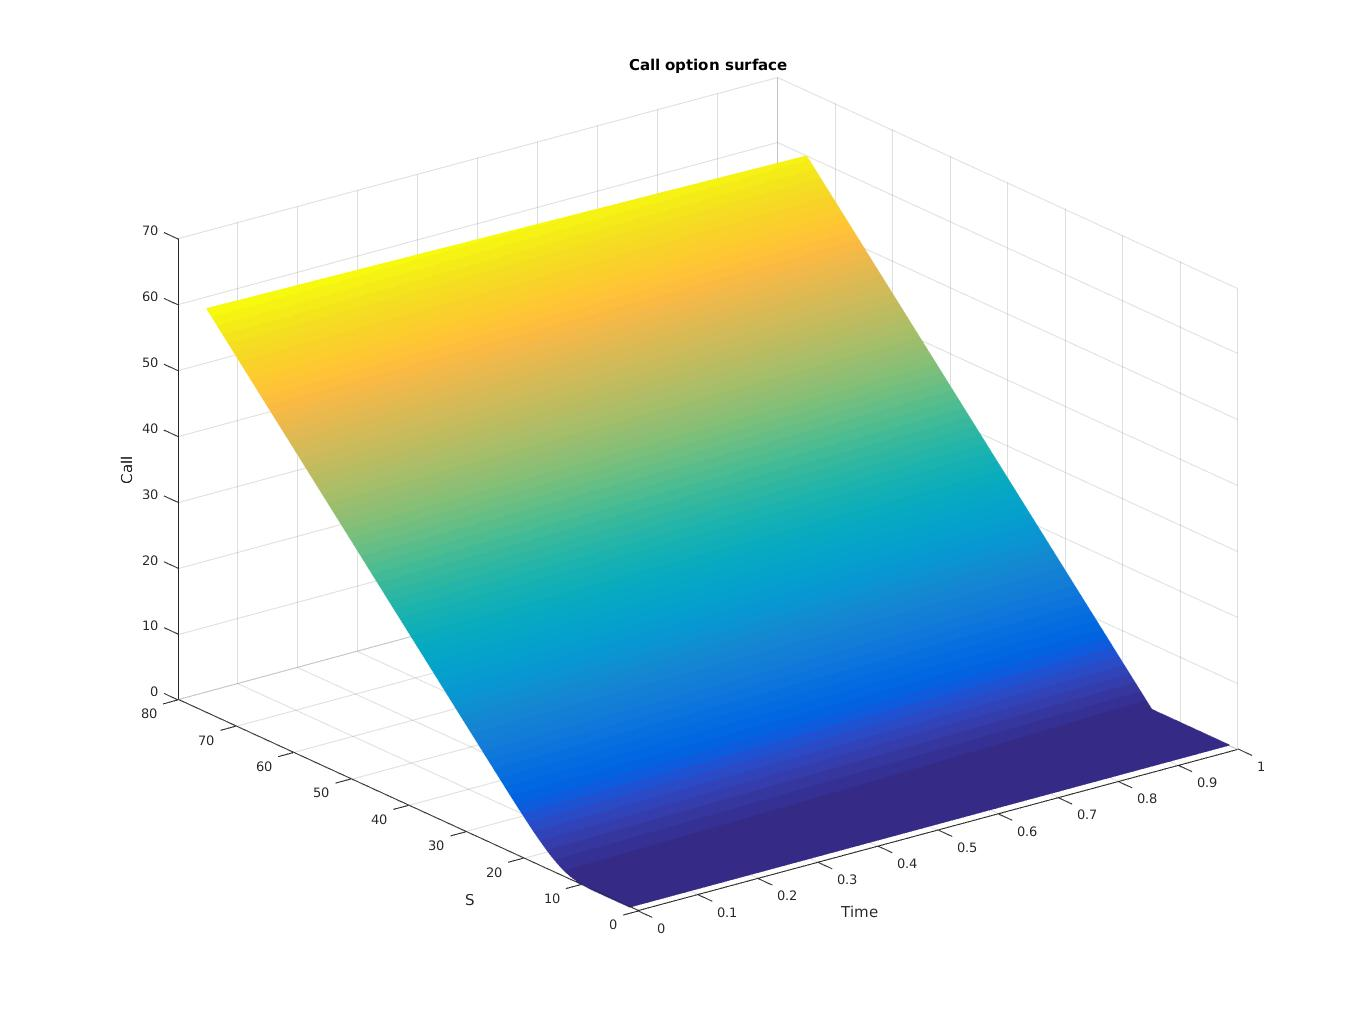
\includegraphics[width=0.8\linewidth]{BS_surface.jpg}
   \caption{Call option surface. It is computed with the parameters in table \ref{tab:BS}}
   \label{BS_surface} 
\end{figure}
$$
\left(
\begin{array}{c}
V^{n+1}_{1} \\
V^{n+1}_{2} \\
\vdots \\
V^{n+1}_{M-2} \\
V^{n+1}_{M-1} \\
\end{array}
\right) = 
\underbrace{
\left(
\begin{array}{ccccc}
b     & c  & 0 & \cdots  & 0 \\
a     & b  & c & 0  & 0  \\
0      & \ddots & \ddots &   \ddots     & 0  \\
\vdots & 0 & a & b  & c  \\
0      & 0 & 0 & a  & b \\
\end{array}
\right) }_{\mathcal{D}} \cdot
\left(
\begin{array}{c}
V^{n}_{1} \\
V^{n}_{2} \\
\vdots \\
V^{n}_{M-2} \\
V^{n}_{M-1} 
\end{array}
\right)
+ \underbrace{
\left(
\begin{array}{c}
 a V^{n}_{0} \\
  0 \\
 \vdots \\
 0 \\
c V^{n}_{M} \\
\end{array}
\right) }_{\mbox{B (boundary terms)}}
$$
The system 
$$ V^{n+1}_{i} = \mathcal{D} V^{n}_{i} + B \quad \mbox{ for } \quad 1 \leq i \leq M-1$$
can be solved easily for $V^{n}_{i}$ by inverting the matrix $\mathcal{D}$.
\begin{figure}[t]
   \centering
   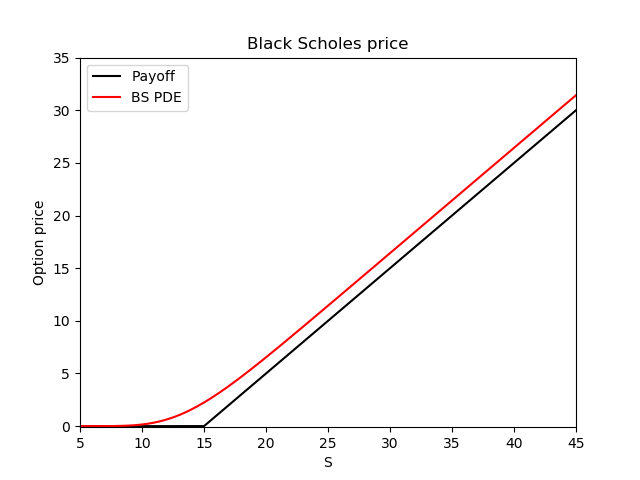
\includegraphics[width=0.7\linewidth]{BS_call.png}
   \caption{Price of a call option at time $t=0$ as a function of the underlying.}
   \label{BS_call}
\end{figure}  
\begin{table}[t]
\begin{center}
\begin{minipage}{0.8\linewidth}
\centering
 \begin{tabular}{||l|l|l|l||}
 \hline
  \multicolumn{4}{|c|}{Diffusion parameters} \\
  \hline
  $K$ & $T$ & $r$ & $\sigma$ \\
  \hline
  15 & 1 & 0.1 & 0.25 \\
  \hline
  \end{tabular}
  \caption{This table shows option's parameters and diffusion process parameters.}
  \label{tab:BS}
\end{minipage}
 \end{center}
\end{table}

Using the parameters in table (\ref{tab:BS}) we solve the fully implicit equation and plot the solution in Figures \ref{BS_surface} and \ref{BS_call}, as an example.



\subsection{Merton PIDE}

\begin{figure}[t]
   \centering
   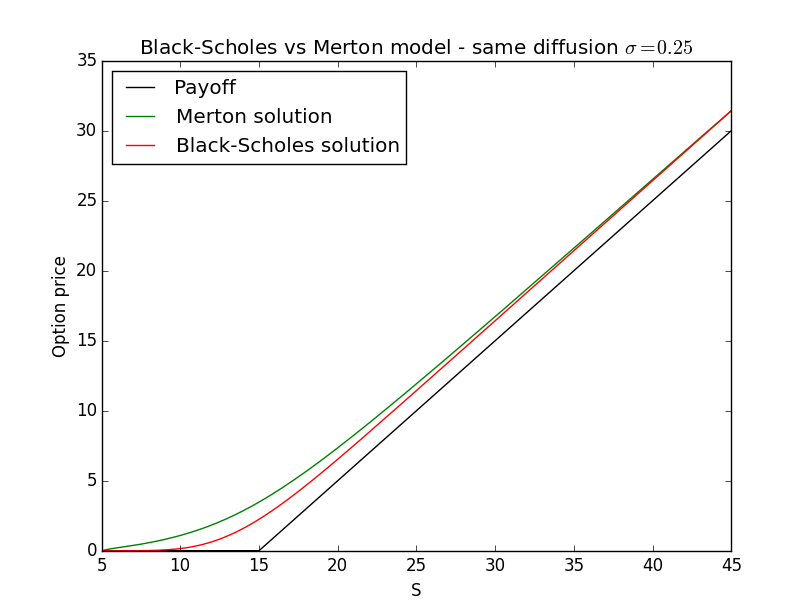
\includegraphics[width=0.7\linewidth]{BS_Merton.png}
   \caption{Comparison of prices of a call option at time $t=0$ for Merton and BS models. The parameter values are those in Tables \ref{tab:Mert} and \ref{tab:BS}}.
   \label{BS_Merton}
\end{figure}  
% \begin{figure}[t]
%    \centering
%    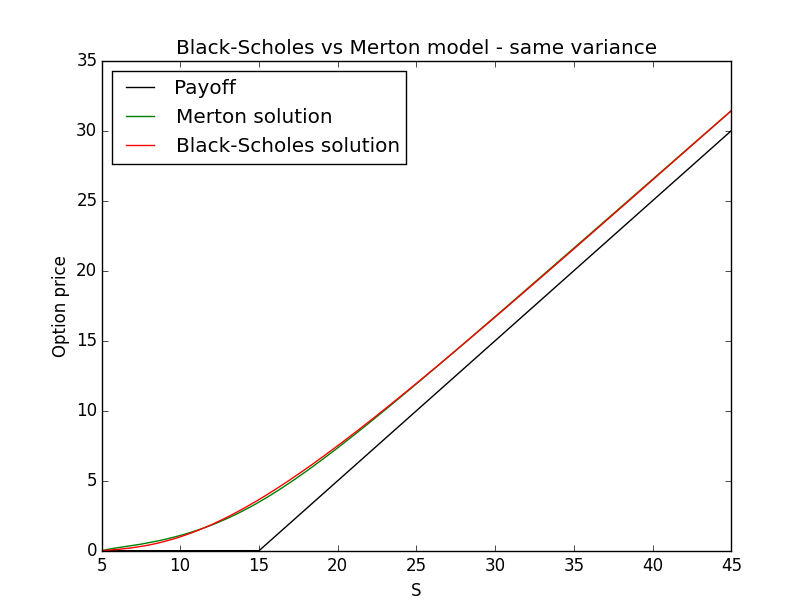
\includegraphics[width=0.7\linewidth]{BS_Merton2.png}
%    \caption{Comparison of prices of a call option at time $t=0$ for Merton and BS models with same standard deviation $=0.25$.}
%    \label{BS_Merton2} 
%  \end{figure}
%  \ \hspace{2mm} \hspace{3mm} \
%  \begin{figure}[t]
%   %\centering
%    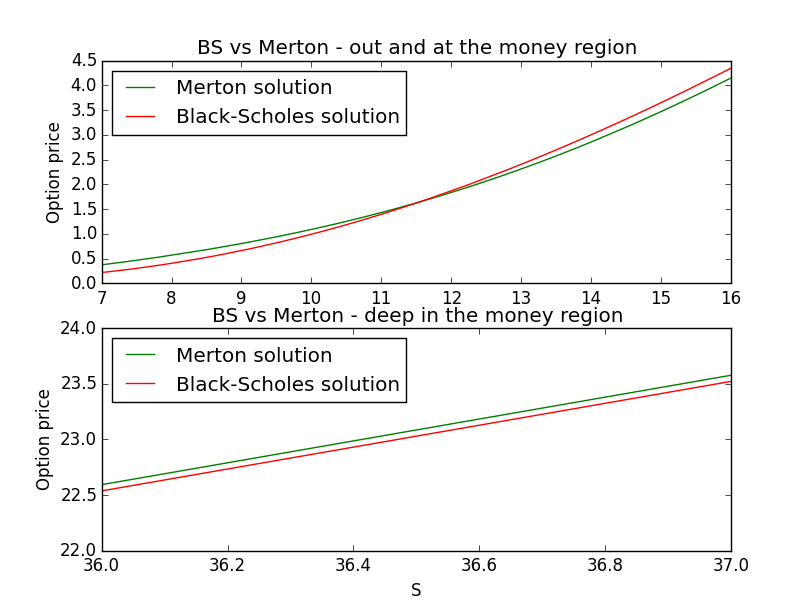
\includegraphics[width=0.7\linewidth]{BS_Merton3.png}
%    \caption{Comparison of prices of a call option at time $t=0$ for Merton and BS models with same standard deviation $=0.25$. Zoom on the ITM and OTM regions.}
%    \label{BS_Merton3}
% \end{figure}
We presented the Merton model in the section (\ref{Merton_section}) and derived the Merton generator in Eq. (\ref{Merton_gen}). 
Recall that the jump component of the Merton process has finite activity, $\nu(\R) = \lambda < \infty$.
Following Eq. (\ref{PIDE_log}), the Merton PIDE in log-variables has the following form: 
\begin{align}\label{Merton_PIDE}
&  \frac{\partial V(t,x)}{\partial t} - r V(t,x) 
          + \biggl( r -\frac{1}{2}\sigma^2 -m \biggr) \frac{\partial V(t,x)}{\partial x} \\ \nonumber
          &+ \frac{1}{2} \sigma^2 \frac{\partial^2 V(t,x)}{\partial x^2} 
          + \int_{\R} V(t,x+z) \nu(dz) - \lambda V(t,x)  = 0.
\end{align}
with $m = \int_{\R} \bigl( e^z-1 \bigr) \nu(dz) = \lambda \bigl( e^{\alpha + \frac{1}{2} \xi^2} -1 \bigr)$. 
But since we have to restrict the unbounded domain to a bounded domain, we consider the equation (\ref{restricted_domain}):
\begin{align*}
&  \frac{\partial V(t,x)}{\partial t} - r V(t,x) 
          + \biggl( r -\frac{1}{2}\sigma^2 - \hat m \biggr) \frac{\partial V(t,x)}{\partial x} \\
          &+ \frac{1}{2} \sigma^2 \frac{\partial^2 V(t,x)}{\partial x^2} 
          + \int_{-B_1}^{B_2} V(t,x+z) \nu(dz) - \hat \lambda V(t,x)  = 0.
\end{align*}
with $\hat m = \int_{-B_1}^{B_2} \bigl( e^z-1 \bigr) \nu(dz)$ and $\hat \lambda = \int_{-B_1}^{B_2} \nu(dz)$.

For $0 < K_1 < K_2$ we choose $B_1,B_2$ such that $ \bigl[-B_1,B_2\bigr] = \bigl[ ( -K_1-1/2 )\Delta x , ( K_2+1/2 )\Delta x \bigr] $.
\begin{equation}\label{trap_quad}
 \int_{-B_1}^{B_2}  V(t_n,x_i+z) \nu(dz) \approx \sum_{k = -K_1}^{K_2} \nu_k V^{n}_{i+k}
\end{equation}
where
\begin{equation}\label{nu1}
 \nu_k = \int_{(k-\frac{1}{2}) \Delta x}^{(k+\frac{1}{2}) \Delta x} \nu(z) dz, \hspace{1em} \mbox{ for } \hspace{1em} -K_1 \leq k \leq K_2. 
\end{equation}
We can derive that $ \hat \lambda = \sum_{k = -K_1}^{K_2} \nu_k $. For large values of $B_1$ and $B_2$, the parameter $\hat \lambda$ is a good approximation for $\lambda$, since
$$\lambda = \lim_{B_1,B_2 \to \infty} \hat \lambda = \lim_{B_1,B_2 \to \infty} \int_{-B_1}^{B_2} \nu(dz).$$
The discretized equation using the IMEX scheme becomes: 
\begin{align}
&\frac{V^{n+1}_{i} -V^{n}_{i}}{\Delta t} + 
(r-\frac{1}{2}\sigma^2 - \hat m) \frac{V^{n}_{i+1} -V^{n}_{i-1}}{ 2 \Delta x} \\ \nonumber
&+ \frac{1}{2} \sigma^2 \frac{V^{n}_{i+1} + V^{n}_{i-1} - 2 V^{n}_{i}}{\Delta x^2}  - (r+\hat \lambda) V^{n}_i +\sum_{k = -K_1}^{K_2} \nu_k V^{n+1}_{i+k} = 0.
\end{align}
Rearranging the terms: 
\begin{align*}
\underbrace{ V^{n+1}_{i} + \Delta t \sum_{k = -K_1}^{K_2} \nu_k V^{n+1}_{i+k} }_{\tilde V^{n+1}_i} &= 
	V^{n}_{i} \biggl( 1 + (r+\hat \lambda)\Delta t + \sigma^2 \frac{\Delta t}{h_x^2} \biggr)  \\
& + V^{n}_{i+1} \biggl( -(r -\frac{1}{2}\sigma^2 -\hat m )\frac{\Delta t}{2 \Delta x} +
\frac{1}{2}\sigma^2 \frac{\Delta t}{\Delta x^2}  \biggr)  \\
& + V^{n}_{i-1} \biggl( (r -\frac{1}{2}\sigma^2 - \hat m)\frac{\Delta t}{2 \Delta x} + 
\frac{1}{2}\sigma^2 \frac{\Delta t}{\Delta x^2}  \biggr).
\end{align*}
We can rename the coefficients:
$$ \tilde V^{n+1}_{i} = a V^{n}_{i-1} + b V^{n}_{i} + c V^{n}_{i+1}, $$
and solve the system for $V^{n}_{i}$:
\begin{equation*}
 \begin{cases}
  \tilde V^{n+1}_i = V^{n+1}_{i} + \Delta t \sum_{k = -K_1}^{K_2} V^{n+1}_{i+k} \nu_k \\
  V^{n}_{i} = \mathcal{D}^{-1} \biggl( \tilde V^{n+1}_{i} - B \biggr) \quad \mbox{ for } \quad 1 \leq i \leq M-1  
 \end{cases}
\end{equation*}
by inverting the tridiagonal matrix $\mathcal{D}$ containing the coefficients $a,b,c$, and with boundary terms $B = (a V^{n}_{0}, 0, ... , 0, c V^{n}_{M})$.  
\begin{table}[t]
 \begin{center}
 \begin{minipage}{0.8\linewidth}
  \centering
  \begin{tabular}{||l|l|l||l|l|l|l||}
  \hline
  \multicolumn{7}{|c|}{Merton parameters} \\
  \hline
  $K$ & $T$ & $r$ & $\sigma$ & $\alpha$ &$\xi$ & $\lambda$ \\
  \hline
  15 & 1 & 0.1 & 0.25 & 0 & 0.5 & 0.8 \\
  \hline
  \end{tabular}
  \caption{This table shows option's parameters and Merton process parameters.}
  \label{tab:Mert}
 \end{minipage}
 \end{center}
\end{table}
In Figure \ref{BS_Merton} we computed the prices using the parameters in tables \ref{tab:Mert} and \ref{tab:BS}. The Merton curve is higher than the BS curve. This is a consequence 
of the presence of a jump component that contributes to the total variance of the process. The two processes have same diffusion component $\sigma$, 
but in the Merton process the total variance is $\sigma^2 + \lambda \xi^2 +\lambda \alpha^2$, while in the BS the variance is just $\sigma^2$.

%In order to compare the two models, we therefore compare two processes with the same variance. The Merton process has parameters as in Table \ref{tab:Mert}, while the BS process has a $\sigma$
%such that it is equal to the standard deviation of the Merton process (see (\ref{Merton_moments}).
%We show the comparison in figures \ref{BS_Merton2} and \ref{BS_Merton3}. We see that under the actual choice of parameters, there is not a very evident difference in the shape.
%However, as expected the BS curve is higher than the Merton curve in the \emph{at the money} (ATM) region, and lower in the deep \emph{in the money} (ITM) 
%and \emph{out of the money} (OTM) regions.
%This is a consequence of the heavy tails distribution of the Merton process, that assigns more probability to the large movements of the underlying.  


\subsection{Variance Gamma PIDE}\label{VG_section2}

The last example we consider is the Variance Gamma process, already introduced in Section \ref{VG_section}. This is an infinite activity process
($\nu(\R) = \infty$). 
If we consider the exponential of the risk neutral process $\{ (r-\omega)t + X_t\}_t$ where $\{X_t\}_t$ is a VG process with triplet as in Section \ref{VG_section}.
By the simple change of variable (\ref{log_var}) on the generator (\ref{VG_gen}), and adding the new term 
$(r-\omega) \frac{\partial V(t,x)}{\partial x}$, we obtain the VG PIDE for a function $V \in C^{1,1}([0,T] \times \R) \bigcap \mathcal{C}_2([0,T] \times \R)$:
\begin{equation} \label{VG_PIDE}
 \frac{\partial V(t,x)}{\partial t} + (r-\omega) \frac{\partial V(t,x)}{\partial x}
 + \int_{\R} \bigl[ V(t,x+z) - V(t,x) \bigr] \nu(dz) = rV(t,x) .
\end{equation}
But in this case, the previous method cannot be applied directly, because of the singularity in the Lévy measure.

The idea for general infinite activity processes is to approximate the process $\{X_t\}_t$ by an
appropriate finite activity process with a modified diffusion component.
We can approximate the ``small jumps'' martingale component with a Brownian motion with the same variance.
After fixing a truncation parameter $\epsilon >0$, we can split the integrals in the SDE into two domains: $\{|z|<\epsilon\}$ and $\{|z|\geq \epsilon\}$.
The integrand on the domain $\{ |z|<\epsilon \}$, is approximated by the Taylor expansion 
 $e^z-1-z = \frac{z^2}{2} + \mathcal{O}(z^3)$ such that
\begin{align}\label{log_sde_inf_act}\nonumber
  dX_t =& \biggl( \mu-\frac{1}{2}\sigma^2 - \int_{\R} \bigl( e^z-1-z \bigr) \nu(dz) \biggr)dt + \sigma dW + + \int_{\R} z \tilde N(dt,dz) \\ \nonumber
       =& \biggl( \mu - \frac{1}{2}\sigma^2 -\int_{|z|<\epsilon} (e^z-1-z) \nu(dz) -\int_{|z|\geq \epsilon} (e^z-1-z) \nu(dz)  \biggr) dt\\ \nonumber
        &+ \sigma dW_t + \underbrace{\int_{|z|< \epsilon} z \tilde N(dt,dz)}_{\sigma_{\epsilon} dW_t} + \int_{|z| \geq \epsilon} z \tilde N(dt,dz) \\ 
       =& \biggl( \mu - \frac{1}{2} (\sigma^2 + \sigma_{\epsilon}^2) - \omega_{\epsilon} + \lambda_{\epsilon} \theta_{\epsilon}  \biggr) dt + \bigl( \sigma+\sigma_{\epsilon}\bigr) dW_t 
       + \int_{|z|\geq \epsilon} z \tilde N(dt,dz) ,
\end{align}
where we defined the new parameters
\begin{align}\label{sig_eps}
 & \sigma_{\epsilon}^2 =  \int_{|z| < \epsilon} z^2 \nu(dz), \quad \quad \omega_{\epsilon} = \int_{|z| \geq \epsilon} (e^z-1) \nu(dz), \\ \nonumber
 & \lambda_{\epsilon} =  \int_{|z| \geq \epsilon} \nu(dz), \quad \quad \theta_{\epsilon} = \frac{1}{\lambda_{\epsilon}} \int_{|z| \geq \epsilon} z \nu(dz) .
\end{align}
The process $\int_{|z|\geq \epsilon} z \tilde N(dt,dz)$ is a compensated Poisson process with finite activity $\lambda_{\epsilon}$ 
and variance $\sigma_J^2 = \int_{|z| \geq \epsilon} z^2 \nu(dz) $.

In the case of the VG process, where $\sigma = 0$ we have the following dynamics for $X_t$
\begin{equation}\label{log_sde_VG}
dX_t = \biggl( \mu - \frac{1}{2} \sigma_{\epsilon}^2 - \omega_{\epsilon} + \lambda_{\epsilon} \theta_{\epsilon}  \biggr) dt 
       + \sigma_{\epsilon} dW_t + \int_{|z|\geq \epsilon} z \tilde N(dt,dz)
\end{equation}
For any $V\in C^2(\R) \bigcap C_2(\R)$, the associated infinitesimal generator has a jump-diffusion form
\begin{align}\label{VG_inf_gen}
\LL^{VG} V(x) \; =& \; \bigl( \mu-\frac{1}{2}\sigma_{\epsilon}^2 - w_{\epsilon} \bigr) \frac{\partial V}{\partial x} 
+ \frac{1}{2}\sigma_{\epsilon}^2 \frac{\partial^2 V}{\partial x^2} \\ \nonumber
&+ \int_{|z| \geq \epsilon} V(x+z) \nu(dz) - \lambda_{\epsilon} V(x).
\end{align}
The same result can be obtained directly from the infinitesimal generator (\ref{RN_log_gen}) with $\sigma =0$:
\begin{align*}
\LL^{VG} V(x) =& \; \mu \frac{\partial V}{\partial x}
+ \int_{|z| < \epsilon}
\biggl[ V(x+z) - V(x) - (e^z-1)\frac{\partial V}{\partial x} \biggr] \nu(dz) \\
&+ \int_{|z| \geq \epsilon}
\biggl[ V(x+z) - V(x) - (e^z-1)\frac{\partial V}{\partial x} \biggr] \nu(dz),
\end{align*}
In the integral term on the domain $\{ |z|<\epsilon \}$, we assume a smooth enough $V$ and use the Taylor approximation
\begin{itemize}
 \item $V(x+z) = V(x) + \frac{\partial V}{\partial x} z + \frac{1}{2} \frac{\partial^2 V}{\partial x^2} z^2 + \mathcal{O}(z^3)$.
 \item $e^z-1 = z + \frac{z^2}{2} + \mathcal{O}(z^3) $.
\end{itemize}
Considering only the terms up to the second order, the integral for $\{ |z| < \epsilon \}$ is
\begin{equation*}
 \int_{|z| < \epsilon} \frac{z^2}{2}
\biggl[ \frac{\partial^2 V}{\partial x^2} - \frac{\partial V}{\partial x} \biggr] \nu(dz)
= \frac{\sigma_{\epsilon}^2}{2} \biggl[ \frac{\partial^2 V}{\partial x^2} - \frac{\partial V}{\partial x} \biggr],
\end{equation*}
and we get again the infinitesimal generator (\ref{VG_inf_gen}).
Using this generator and equations (\ref{derivative_PIDE}) and (\ref{mu=r}), the final PIDE is thus
\begin{figure}[!t]
   \centering
   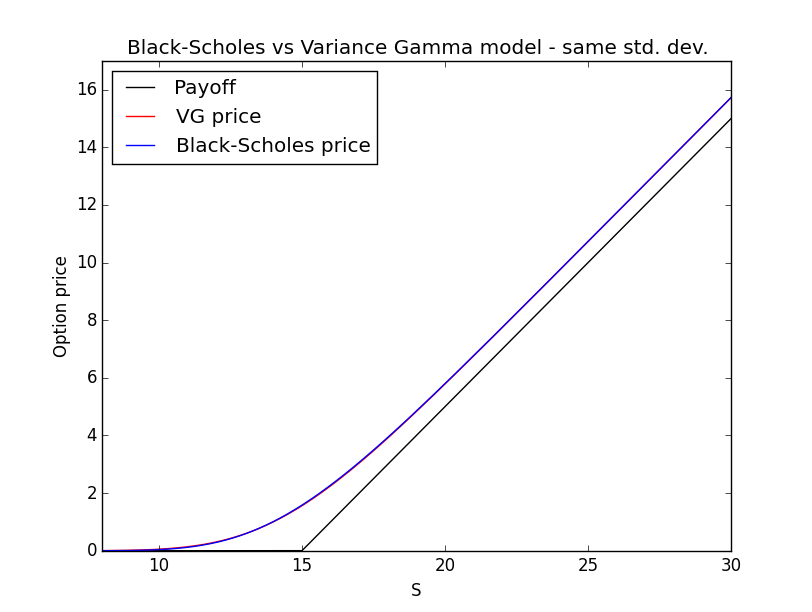
\includegraphics[width=0.7\linewidth]{BS_VG.png}
   \caption{Comparison of prices of a call option for VG and BS models. The VG curve is computed with the parameter values in (\ref{tab:VG}). The BS curve is computed with a 
   value $\sigma = 0.2024$, such that the two processes have same variance.}
   \label{BS_VG} 
 \end{figure}
\begin{align}\label{VG_JD}
&  \frac{\partial V(t,x)}{\partial t} +
 \bigl( r-\frac{1}{2}\sigma_{\epsilon}^2 - w_{\epsilon} \bigr) \frac{\partial V(t,x)}{\partial x} 
 + \frac{1}{2}\sigma_{\epsilon}^2 \frac{\partial^2 V(t,x)}{\partial x^2} \\ \nonumber
 &+ \int_{|z| \geq \epsilon} V(t,x+z) \nu(dz) = (\lambda_{\epsilon} + r) V(t,x).
\end{align}
This equation is very similar to equation (\ref{Merton_PIDE}), except for the truncation in the integral. 
At this point we can restrict the computational domain on $[A_1,A_2]$ and the integral region on $[-B_1,B_2]$ and using the same discretization
used for the Merton PIDE, we can solve the problem with the IMEX scheme.\\
\begin{table}[h!]
\begin{center}
 \begin{minipage}{0.8\linewidth}
  \centering
 \begin{tabular}{||l|l|l|l||l|l||}
\hline
  \multicolumn{6}{|c|}{VG parameters} \\
 \hline
$K$ & $T$ & $r$ & $\theta$ & $\bar\sigma$ &$\kappa$  \\
\hline
15 & 1 & 0.1 & -0.1 & 0.2 & 0.1 \\
\hline
\end{tabular}
  \caption{This table shows option's parameters and VG process parameters.}
  \label{tab:VG}
\end{minipage}
  \end{center}
\end{table}
Using the parameters in Table \ref{tab:VG} we compute the call option prices for the VG process and compare them with the prices of a BS process with the same variance.
In this way the features coming from skewness and kurtosis should pop up.  
In figure \ref{BS_VG} we show the comparison between the two curves, but under this choice of parameters, the difference in the shapes is not very evident.

The reader can consult \cite{Schoutens} for further numerical tests on the calibration of exponential Lévy processes, such as Merton and VG processes. 






\chapter{Multinomial methods for Variance Gamma}\label{Chapter3}
%\blindtext
\minitoc% Creating an actual minitoc

\vspace{5em}


 
 
In this thesis we decided to work with the Variance Gamma (VG) process because it has nice analytical properties and 
it reproduces quite well the statistical features of the stock dynamics (see for instance \cite{Cont} and \cite{Ait12}).

To support this statement, 
we present in Figure \ref{FigPDF} some examples of histograms of
daily log-returns of the four indices:  
the \textbf{S\&P 500} Stock Index, 
the \textbf{KOSPI} (Korea Composite Stock Price Index), 
\textbf{XAO} (All Ordinaries Australian Index)  
and \textbf{TAIEX} (Taiwan Capitalization weighted Stock Index).
In the pictures we show the fit of the Normal and Variance Gamma (VG) densities, using the market data. 
It is clear that the 
VG density reproduces much better the high peaks near the origin and the heavy tails of the empirical distribution.

\begin{figure}[t!]
 \centering
 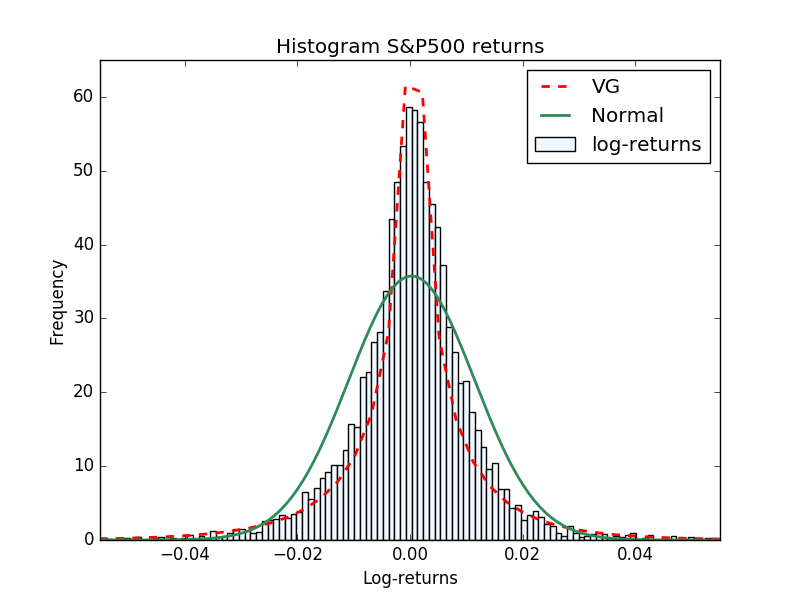
\includegraphics[width=0.47\textwidth]{sp500.png}
 ~
 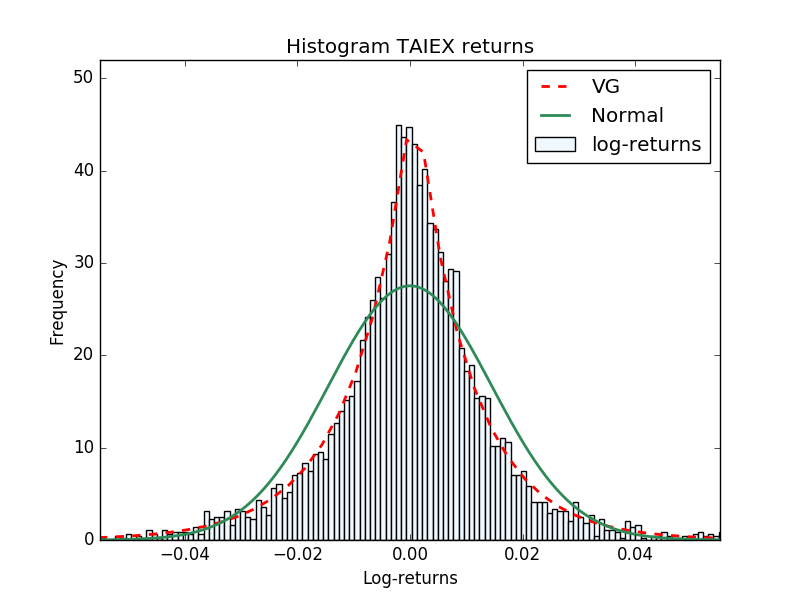
\includegraphics[width=0.47\textwidth]{twii.png}
 ~
 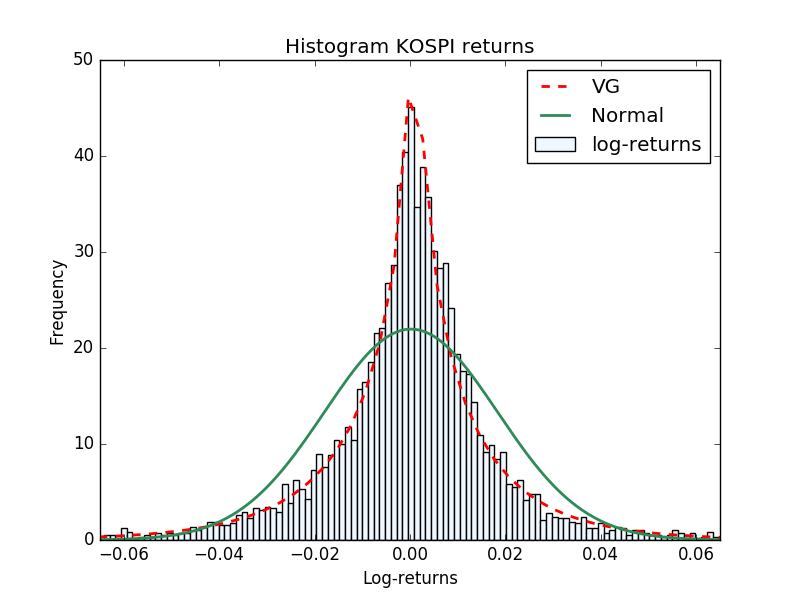
\includegraphics[width=0.47\textwidth]{kospi.png}
 ~
 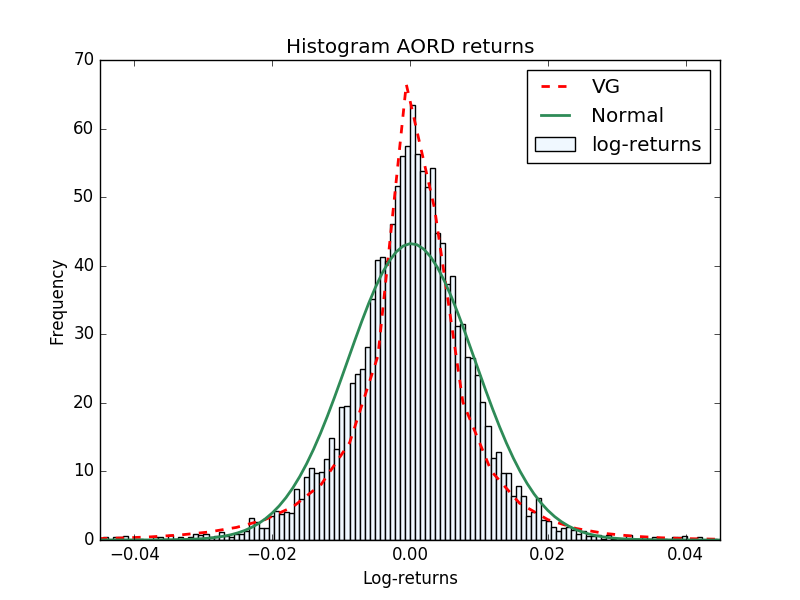
\includegraphics[width=0.47\textwidth]{xao.png}
 % VG4_pdf.png: 0x0 pixel, 0dpi, 0.00x0.00 cm, bb=
 \caption{Histograms of daily log-returns for S\&P500, KOSPI, XAO and TAIEX, from 1 January 1988 to 9 December 2016. Source: Yahoo Finance.
 The dashed line corresponds to the VG density (\ref{VG_density}). 
 The continuous line is the normal density. 
 The parameters are obtained by the \emph{method of moments}. For more details on the parameter estimation for the VG density we refer to \cite{Se04}.}
 \label{FigPDF}
\end{figure} 

The VG process was first presented in the context of option pricing 
in \cite{MaMi91}, where it has been used for pricing European options.
European vanilla options can be easily priced by the analytical formula presented in \cite{MCC98} and exotic options
can be priced numerically by several common techniques.
Monte Carlo methods for VG are presented in \cite{Fu00}. 
A finite difference scheme for the VG Partial Integro-Differential Equation (PIDE) 
is described in \cite{CoVo05b}. In \cite{CaMa98}, the authors show how to price options by a Fourier transform approach.
The problem for American options is considered in \cite{Al05}, \cite{Oo05} and \cite{HiMa01}, where the authors present different finite difference 
schemes to solve the American VG PIDE.

The tree method was first introduced by \cite{CRR79} for a market where the log-price can change only in two different ways: 
an upward jump, or a downward jump. For this reason the model is called \emph{binomial model}. The authors 
prove that when the number of time steps goes to infinity, the discrete random walk of the log-price converges to the Brownian motion
and the option price converges to the Black-Scholes price.
The \emph{multinomial model} is a generalization of the binomial model, and at each time step it considers 
more than just two possible future states.
A general multinomial method for pricing European and American options under exponential L\'evy processes is described in \cite{MaSoSz}. 
In \cite{KeWe06} the authors consider a multinomial method for general exponential L\'evy processes based on the moment matching condition.
Other methods based on the moment matching condition are for instance \cite{HaMac10}, with applications to the Normal Inverse Gaussian process, and 
\cite{See13} with applications to the VG process.  
In the present work we consider a multinomial discretization based on the cumulant matching condition as explained in \cite{YaPr01}, \cite{YaPr03} and \cite{YaPr06}. 


In Section \ref{sec3_ch3} we review the construction of the multinomial tree, following the method of
moment matching proposed in \cite{YaPr01}. We prove that the multinomial tree converges to the continuous time jump process that we have
introduced to approximate the VG process.
In Section \ref{sec4_ch3}, we describe the algorithm for pricing options with the 
multinomial method and show the numerical results for European and American options.




\section{The multinomial method} \label{sec3_ch3}
In this section we introduce the multinomial method proposed in \cite{YaPr06}. 
The stock price is represented by a Markov chain with $L$ possible future states at each time. 
In this setting, the time $t \in [t_0,T]$ is discretized as $t_n = t_0 + n\Delta t$ for $n=0, ... ,N$ and 
$\Delta t = (T-t_0)/N$. We denote the stock price at time $t_n$ as $S_{t_n} = S_n$.

Let us consider the up/down factors $u>d>0$, and write the discrete evolution of the stock price $S_n$ as:
\begin{equation}\label{Discr_S}
  S_{n+1} = u^{L-l}d^{l-1} S_n  \hspace{3em} l=1, ... , L  
\end{equation}
where each future state has transition probability $p_l$, satisfying $\sum_{l=1}^L p_l = 1$.
The value of the stock at time $t_n$ can assume $j \in [1,...,n(L-1)+1]$ possible values:
\begin{equation}\label{Discr_S2}
  S_{n}^{(j)} = u^{n(L-l)+1-j}d^{j-1} S_0.  
\end{equation}
The multinomial tree is recombining if $u/d = c$, for $c>1$.
In the present work we only consider five branches, $L=5$. As we will see in the next sections this number of branches is 
enough to model the features of a stochastic process up to its fourth moment.


\subsection{Moment matching}

In order to determine the parameters of the Markov chain we require that its local moments are equal to that of the continuous process.
Let us consider a VG process with drift $(r-w)$, where $w$ is the martingale correction defined in (\ref{parameter_w}): 
%and derive the continuous process for the log-variable $Y_t = \log(S_t)$: 
\begin{align}\label{log_martingale}
 Y_{t+\Delta t}-Y_t &= (r-w)\Delta t + \int_{\R} x N(\Delta t,dx) \\ \nonumber
		    &= (r-w + \theta)\Delta t + \int_{\R} x \tilde N(\Delta t,dx)
\end{align}
The parameter $\theta = \int_{\R} x \nu(dx) = \E \bigl[ \int_{\R} x N(1,dx) \bigr]$ is the expected value of the VG process in (\ref{VG_process}), 
when $\Delta t=1$. 
The integral with respect to the compensated Poisson measure $\tilde N(\Delta t,dx)$ is a martingale as discussed in Section \ref{random_measures}.

We can pass to log-prices $Y_n = \log(S_n)$ in the discrete Eq. (\ref{Discr_S}), and write it as the sum of a drift component and a 
random variable with $L$ possible outcomes:
\begin{align}\label{Discr_Y}
 \Delta Y = Y_{n+1} - Y_n &= (L-l) \log(u) + (l-1) \log(d) \\ \nonumber
  &= \bar b\, \Delta t + (L-2l+1) \alpha(\Delta t).
\end{align}
The term $\bar b\, \Delta t$ is the drift term, while the term $l$ is a random variable that takes values in $\{1,2,...,L\}$ with probability $p_l$. 
It has to satisfy the martingale condition:
$$ \E \bigl[(L-2l+1) \alpha(\Delta t) \bigr] = \alpha(\Delta t) \sum_{l=1}^L p_l (L-2l+1) = 0, $$
and $\alpha(\Delta t)$ is a function of $\Delta t$.

The corresponding up/down factors have the following representation:
\begin{equation}\label{updown}
 u = \exp\biggl( \frac{b}{L-1} + \alpha(\Delta t) \biggr) \hspace{2em}  d = \exp\biggl( \frac{b}{L-1} - \alpha(\Delta t) \biggr),
\end{equation}
and we can readily see that if $u/d$ is a constant, then the tree recombines.

Given the mean $c_1 = \E[\Delta Y] = \bar b \Delta t$, the $k$-central moment is:
\begin{equation}\label{higher_moments}
 \E \bigl[ (\Delta Y - c_1)^k \bigr] = \alpha(\Delta t)^k\, \E \bigl[ (L-2l+1)^{k} \bigr].
\end{equation}
The moment matching condition requires that the central moments of the discrete process (\ref{Discr_Y}) 
are equal to the central moments
of the continuous process (\ref{log_martingale}):
\begin{equation}\label{moment_matching}
 \alpha(\Delta t)^k\, \E \bigl[ (L-2l+1)^{k} \bigr] = \mu_k.
\end{equation}
We fix $L=5$, and using the relation between central moments and cumulants (Eq. (\ref{moment_cumulants}) )
we solve the linear system of equations for the transition probabilities:
\begin{align}\label{probabilities1}
 p_1 &= \frac{1}{196 \alpha(t)^4} \biggl[ \frac{3}{2} c_2^2 -2 c_2\alpha(t)^2 + 2 c_3 \alpha(t) +\frac{1}{2} c_4  \biggr] \\ \nonumber
 p_2 &= \frac{1}{196 \alpha(t)^4} \biggl[ -6 c_2 + 32c_2 \alpha(t)^2 - 4c_3 \alpha(t) -2 c_4 \biggr] \\ \nonumber
 p_3 &=  1 + \frac{1}{196 \alpha(t)^4} \biggl[ 3c_4 + 9c_2^2 -60c_2 \alpha(t)^2   \biggr] \\ \nonumber
 p_4 &= \frac{1}{196 \alpha(t)^4} \biggl[ -6 c_2 + 32c_2 \alpha(t)^2 + 4c_3 \alpha(t) -2 c_4  \biggr] \\ \nonumber
 p_5 &= \frac{1}{196 \alpha(t)^4} \biggl[ \frac{3}{2} c_2^2 -2 c_2\alpha(t)^2 - 2 c_3 \alpha(t) +\frac{1}{2} c_4 \biggr].
\end{align}
The drift parameter corresponds to $\bar b = r - w + \theta$.
The only missing term to find is $\alpha(\Delta t)$. This is a function of the time increment $\Delta t$ and can be determined using the 
higher order terms in the moment matching condition together with the condition of positive probabilities.

Recall that the well known binomial model \cite{CRR79} assumes the value $\alpha(\Delta t) = \sigma \sqrt{\Delta t}$,
that represents the volatility of the increments in the time interval $\Delta t$.
In the trinomial model, the parameter $\alpha(\Delta t)$ assumes the value $\alpha(\Delta t) = \frac{1}{2} \sigma \sqrt{3\Delta t}$, see for instance \cite{YaPr01}.
For the multinomial method a good representation for $\alpha(\Delta t)$ is:
\begin{equation}\label{alphat}
 \alpha(\Delta t) = \sqrt{c_2} \sqrt{\frac{3+\bar \kappa}{12}},
\end{equation}
where $\bar \kappa = c_4 / c_2^2$ is the excess of kurtosis\footnote{We use the bar over $\kappa$, 
to distinguish the kurtosis from the variance of the gamma process $\kappa$.}. 
We refer to \cite{YaPr06} for the derivation.
This choice guarantees that the probabilities $p_i$ for $i=1...5$ are always positive and sum to one. We can replace the expression
(\ref{alphat}) inside (\ref{probabilities1}), to obtain the simpler form:
\begin{align}\label{probabilities2}
 & [p_1,p_2,p_3,p_4,p_5] \approx \biggl[ \frac{3+\bar \kappa+s\sqrt{9+3\bar \kappa}}{4(3+\bar \kappa)^2} , 
 \frac{3+\bar \kappa-s\sqrt{9+3\bar \kappa}}{2(3+\bar \kappa)^2} , \\ \nonumber
 &
 \frac{3+2\bar \kappa}{2(3+\bar \kappa)} ,
 \frac{3+\bar \kappa+s\sqrt{9+3\bar \kappa}}{2(3+\bar \kappa)^2} ,
 \frac{3+\bar \kappa-s\sqrt{9+3\bar \kappa}}{4(3+\bar \kappa)^2} \biggr],
\end{align}
where $s = c_3 / \sqrt{c_2^3}$ is the skewness.
\begin{Remark}
 The standard deviation of every L\'{e}vy process with finite second moment follows the square root propagation rule. This means that the term $\alpha(\Delta t)$ has to be proportional
 to the square root of $\Delta t$. In the binomial and trinomial models, the proportionality constant is explicit, while for the pentanomial method it is implicit
 in the formula (\ref{alphat}). Expanding the formula using the expression (\ref{VG_cumulants}) for the cumulants, it is possible to check that the square root rule is
 satisfied at first order in $\sqrt{\Delta t}$.
\end{Remark}



\subsection{Convergence}


We call a generic jump process (\ref{Levy_Ito3}) with first four cumulants $c_1$,$c_2$,$c_3$,$c_4$ as in (\ref{VG_cumulants}), 
the \emph{approximated process} $X^A$. 
The cumulant generating function of the increment $\Delta X^A$ has the following series representation (see Section \ref{cumulant_sec} ):
\begin{equation}\label{cum_gen_appr}
 H_{\Delta X^{A}}(u) = ic_1 u -\frac{c_2u^2}{2} -\frac{ic_3u^3}{3!} + \frac{c_4u^4}{4!} + \mathcal{O}(u^5).
\end{equation}
We are interested in the approximation of a VG process with drift (\ref{log_martingale}), therefore we require that $c_1 = \bar b \Delta t = (r-w+\theta)\Delta t$. 
\begin{Theorem}
The increments of the discrete Markov chain (\ref{Discr_Y}) and the increments of the approximated process $X^A$ have the same distribution by construction.
\end{Theorem}
\begin{proof}
The idea of the proof is to show that the cumulant generating function of the discrete process (\ref{Discr_Y}) 
coincides with that of the approximated process (\ref{cum_gen_appr}). We prove it by using the moment
matching condition (\ref{moment_matching}).
\begin{align}
H_{\Delta Y}(u) &= \log \bigl( \phi_{\Delta Y}(u)  \bigr) = \log \biggl( \E \bigl[ e^{iu \Delta Y} \bigr] \biggr) \\ \nonumber
                &= \log \biggl( \E \biggl[ e^{iu \bigl( \bar b \Delta t + (L-2l+1) \alpha(\Delta t) \bigr) } \biggr] \biggr) \\ \nonumber
		&= iu \bar b \Delta t + \log \biggl( \E \biggl[ e^{iu \bigl(  (L-2l+1) \alpha(\Delta t) \bigr) } \biggr] \biggr).
\end{align}
We can expand the exponential function in Taylor series and use the moment matching condition (\ref{moment_matching}) to obtain:
\begin{align}
H_{\Delta Y}(u) &= iu \bar b \Delta t + \log \biggl( \sum_{k=0}^{\infty} \frac{(iu)^k}{k!} 
\bigl(\alpha(\Delta t)\bigr)^k \E \biggl[ \bigl( L-2l+1  \bigr)^k \biggr] \biggr) \\ \nonumber
                &= iu \bar b \Delta t + \log \biggl( \sum_{k=0}^{\infty} \frac{(iu)^k}{k!} \mu_k \biggr) \\ \nonumber
                &= iu c_1 + \sum_{k=0}^{\infty} \frac{(iu)^k}{k!} c_k \\ \nonumber 
                &= H_{\Delta X^{A}}(u),
\end{align}
\end{proof}
\begin{Remark}
All the cumulants of $\Delta X^A$ are equal to the cumulants of the Markov chain (\ref{Discr_Y}) by construction, but only the first four are equal to the VG cumulants.
When all the cumulants $c_i$, for $0 \leq i \leq n$, are equal to the VG cumulants, the approximated process $X^A$ converges to
the original VG process for $n \to \infty$.
In order to describe $n$ cumulants, we need $n+1$ branches. Therefore, when the number of cumulants of $\Delta X^A$ that are equal to those of the VG goes to infinity, 
the number of branches has to go to infinity as well.
We assume that five branches ($L=5$) are enough to describe the main features of the underlying process and, at the same time, keep the numerical
problem simple. 
\end{Remark}

\begin{Theorem}
The distribution of the pentanomial tree at time $N$ converges to the distribution of a compound Poisson process at time $N$ with $L=5$ possible jump sizes and activity $\lambda = \frac{3}{2 \bar \kappa N}$, when $\Delta t \to 0$.   
\end{Theorem}
For the proof of this theorem  
we refer to Section 4.2 of \cite{YaPr06}. The authors first define the jump sizes and their respective probabilities, and then
prove that when $\Delta t \to 0$ the characteristic function of the pentanomial tree converges to the 
characteristic function of the compound Poisson process.



\section{Numerical results} \label{sec4_ch3}

In this section we present the steps to implement the algorithm for pricing European and American options with the multinomial method.
Then we compare the results with those obtained by the PIDE method and Black-Scholes model.

\subsection{Algorithm}

We suggest the following algorithm for pricing with the multinomial method:
\begin{enumerate}
 \item Compute the transition probabilities vector (\ref{probabilities2}). 
 \item Compute the up/down factors $u$ and $d$ (\ref{updown}) and the vector of prices $S_N$ at terminal time $N$ as in Eq. (\ref{Discr_S2}).
 \item Evaluate the payoff of the option $V^N(S_N)$ at terminal time $N$.
 \item Given the option values at time $t_{n+1}$ compute the values at time $t_n$. The value is the conditional expectation:
 \begin{equation}
 V^n(s^{(k)}_n) = e^{-r\Delta t} \E^{\Q} \biggl[ V^{n+1}(S_{n+1}) \bigg| S^{(k)}_n = s^{(k)}_n \biggr]. 
\end{equation}
 \item If computing the price of an American option, the value at the previous time level is the maximum between the conditional expectation and
 the intrinsic value of the option. For an American put we have:
 \begin{equation}
 V^n(s^{(k)}_n) = \max \biggr \{ e^{-r\Delta t} \E^{\Q} \biggl[ V^{n+1}(S_{n+1}) \bigg| S^{(k)}_n = s^{(k)}_n \biggr] , K-s^{(k)}_n \biggr \}. 
\end{equation}	
 \item Iterate the algorithm until the initial time $t_0$. 
\end{enumerate}

In all the numerical computations of this chapter we consider the risk neutral VG parameters in Table \ref{sample-table}. These parameters correspond to the parameters used 
in \cite{Canta2}.

\begin{table}[!h]
\centering
{\begin{tabular}{llll}
\toprule
 \multicolumn{4}{c}{Parameters} \\
\midrule
$r$ & $\theta$ & $\sigma$ & $\kappa$ \\ 
0.06 & -0.1 & 0.2 & 0.2 \\
\bottomrule
\end{tabular}}
\caption{$r$ is the risk free interest rate and $\theta, \sigma, \kappa$ are the risk neutral VG parameters.}
\label{sample-table}
\end{table}

\begin{Remark}
In practice, the risk neutral parameters of the VG model should be calibrated from market prices of European vanilla options, using the closed pricing formula of \cite{MCC98}.
Then, this risk neutral VG model can be used to price exotic derivatives for which there are no closed formulas.
The multinomial method is particularly suitable for American-style options, since Monte Carlo and PIDEs methods are in general more difficult to implement. 
For this reason, tree methods are quite popular among practitioners. 
\end{Remark}







\subsection{European options}


We compare the numerical results for European call and put options obtained with the multinomial and the PIDE approaches.
We solve the VG PIDE following the IMEX method introduced in Section \ref{VG_section2}.
The details of the implementation are presented in Section \ref{numerical_concergence_section}. 

Following the algorithm proposed in the previous section, we solve the option pricing problem using the multinomial method. 
The number of time steps for all the computations presented in the following pictures is $N=2000$. 
The Table \ref{Convergence} 
shows a convergence analysis for the prices of European calls, puts and American puts. We can see that the convergence is quite fast.  
\begin{table}[ht]
\centering
{\begin{tabular}{llllll}
\toprule
  $N$ & Eu. Call & Eu. Put & Time & Am. Put & Time \\
\midrule
    50 & 4.41873125 & 2.08928091 & 0.001 & 2.36765911 & 0.007 \\
    100 & 4.41960265 & 2.09015381 & 0.002 & 2.37255454 & 0.02 \\
    200 & 4.41997010 & 2.09052201 & 0.004 & 2.37480218 & 0.07 \\
    400 & 4.42013640 & 2.09068869 & 0.01 & 2.37587117 & 0.29 \\
    800 & 4.42021515 & 2.09076762 & 0.03 & 2.37639131 & 1.09 \\
    1000 & 4.42023054 & 2.09078306 & 0.04 & 2.37649417 & 1.67 \\
    1500 & 4.42025089 & 2.09080345 & 0.06 & 2.37663070 & 3.79 \\
    2000 & 4.42026098 & 2.09081357 & 0.10 & 2.37669869 & 6.80 \\
    2500 & 4.42026701 & 2.09081962 & 0.16 & 2.37673941 & 10.65 \\
    3000 & 4.42027102 & 2.09082364 & 0.2 & 2.37676652 & 14.78 \\
  \bottomrule
\end{tabular}}
\caption{Convergence table for ATM European and American options with strike $K=40$ and $T=1$. The time unit is in seconds.}
\label{Convergence}
\end{table}
Figures \ref{figCall} and \ref{figPut} show the single prices obtained by the multinomial method compared with the curve obtained by solving the PIDE.
In Table \ref{Option_values} we compare directly the call/put numerical values obtained with the two methods.
\begin{figure}[t!]
 \begin{minipage}[b]{0.5\linewidth}
   \centering
 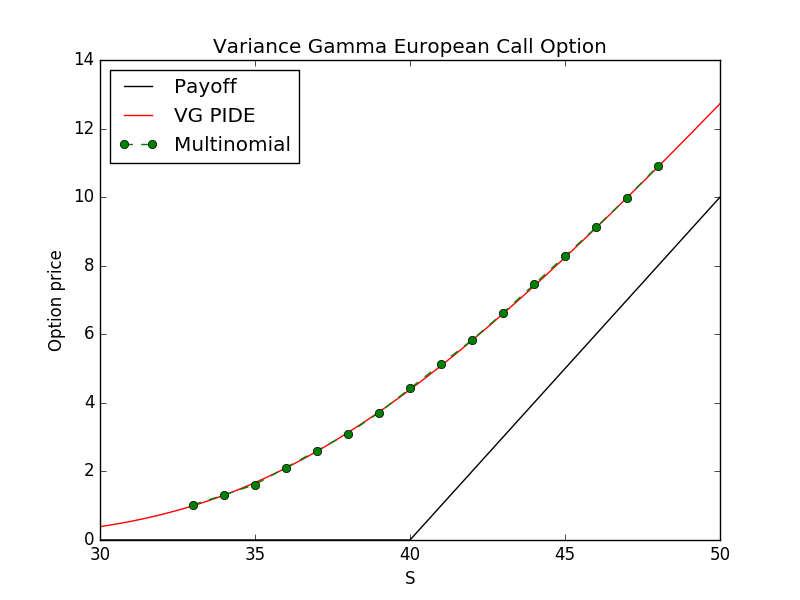
\includegraphics[width=\linewidth]{EU_call.png}
 % EU_call.png: 0x0 pixel, 300dpi, 0.00x0.00 cm, bb=
 \caption{European call option with strike $K=40$ and time to maturity 1 year.}
 \label{figCall}
  \end{minipage}
 \ \hspace{2mm} \hspace{3mm} \
 \begin{minipage}[b]{0.5\linewidth}
 \centering
 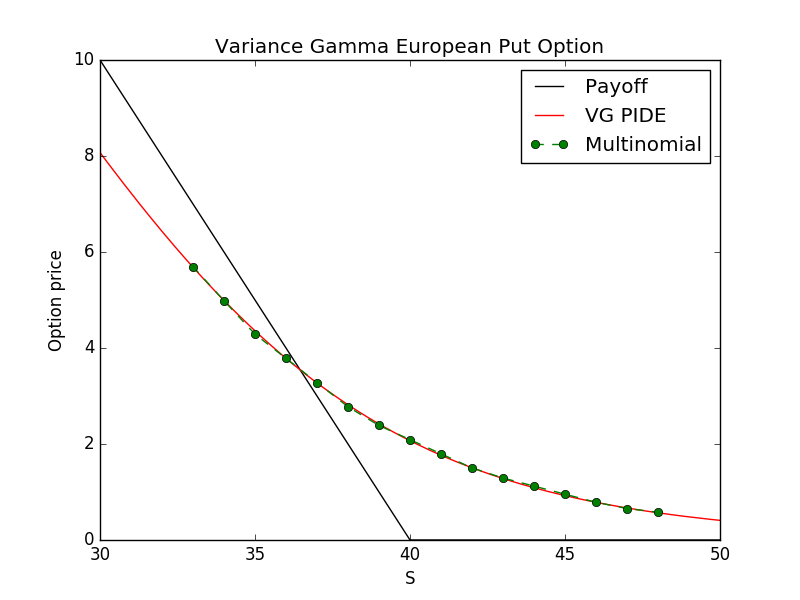
\includegraphics[width=\linewidth]{EU_put.png}
 % EU_call.png: 0x0 pixel, 300dpi, 0.00x0.00 cm, bb=
 \caption{European put option with strike $K=40$ and time to maturity 1 year.}
 \label{figPut}
 \end{minipage}
\end{figure}

\begin{table}[ht]
\centering
{\begin{tabular}{lllll} 
\toprule
\multicolumn{5}{c}{Different methods} \\
\midrule
$S_0$ & PIDE Call & Multi Call & PIDE Put & Multi Put \\
\midrule
36 & 2.1036 & 2.1131 & 3.7842 & 3.7837  \\
  38 & 3.1163 & 3.1051 & 2.7893 & 2.7756 \\
  40 & 4.4162 & 4.4203 & 2.0852 & 2.0908 \\
  42 & 5.8335 & 5.8309 & 1.5050 & 1.5014 \\
  44 & 7.4417 & 7.4524 & 1.1132 & 1.1229 \\
\bottomrule
\end{tabular}}
\caption{European Options, with strike $K=40$ and $T=1$.}
\label{Option_values}
\end{table}



\subsection{American options}

In this section we present the numerical results obtained with the multinomial method algorithm for American put options, and compare them with the PIDE method (see fig. \ref{AmVG}).
The PIDE (\ref{VG_JD}) is modified in order to take into account the early exercise feature:
\begin{align}\label{VG_Am_JD}
&  \min \biggl\{ - \frac{\partial V(t,x)}{\partial t} -
 \bigl( r-\frac{1}{2}\sigma_{\epsilon}^2 - w_{\epsilon} \bigr) \frac{\partial V(t,x)}{\partial x} 
 - \frac{1}{2}\sigma_{\epsilon}^2 \frac{\partial^2 V(t,x)}{\partial x^2} + (\lambda_{\epsilon} + r) V(t,x) \\ \nonumber
 &- \int_{|z| \geq \epsilon} V(t,x+z) \nu(dz) \, , \, \biggl( V(t,x) - (K-e^x)^+ \biggr) \biggr\} = 0.
\end{align}
To solve this equation we use the same discretization and same settings used in Sections \ref{VG_section2} and \ref{numerical_concergence_section} for the European option problem.

The numerical values obtained by multinomial and PIDE methods are collected in Tab. \ref{Option_values3}.
The run times for the multinomial algorithm are shown in the convergence Table \ref{Convergence}.
\begin{figure}[ht!]
 \centering
 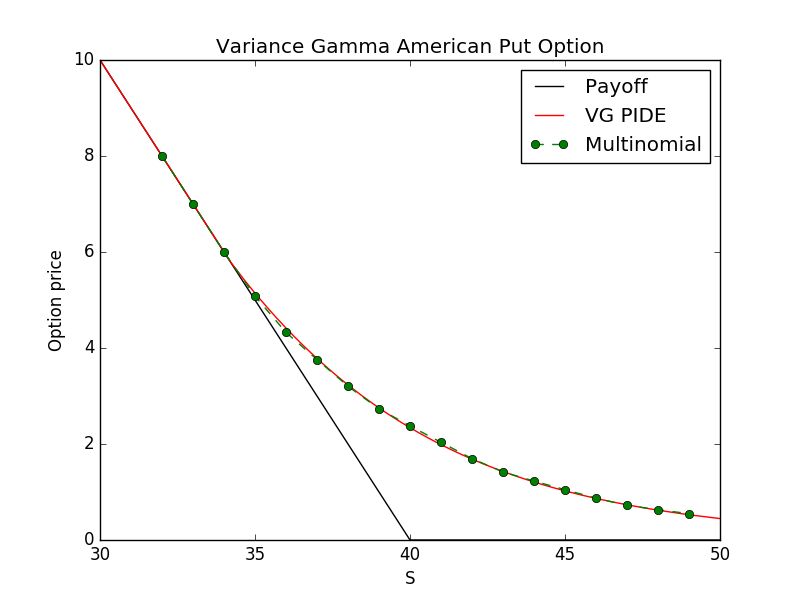
\includegraphics[scale=0.4]{American_VG.png}
 % EU_call.png: 0x0 pixel, 300dpi, 0.00x0.00 cm, bb=
 \caption{American put option with strike $K=40$ and time to maturity 1 year. Comparison of PIDE prices and multinomial prices.}
 \label{AmVG}
\end{figure}
\begin{table}[ht]
{\begin{tabular}{llllll}
\toprule
 \multicolumn{6}{c}{Prices comparison} \\
\midrule
$S_0$ & BS Eu. Put & VG Eu. Put & BS Am. Put & VG Am. Put & VG Am. PIDE Put \\
 \midrule
  30 & 8.1316 & 8.0809 & 10     & 10     & 10 \\
  32 & 6.5292 & 6.4055 & 8      & 8      & 8 \\
  34 & 5.1169 & 4.9851 & 6.0894 & 6      & 6 \\
  36 & 3.9150 & 3.7837 & 4.5415 & 4.3173 & 4.3982 \\
  38 & 2.9263 & 2.7756 & 3.3264 & 3.2034 & 3.2195 \\
  40 & 2.1388 & 2.0908 & 2.3924 & 2.3767 & 2.3531 \\
  42 & 1.5322 & 1.5014 & 1.6911 & 1.6947 & 1.6849 \\
  44 & 1.0766 & 1.1229 & 1.1755 & 1.2267 & 1.2118 \\
  46 & 0.7433 & 0.7858 & 0.8043 & 0.8699 & 0.8650 \\
  48 & 0.5049 & 0.5787 & 0.5425 & 0.6310 & 0.6221 \\
  50 & 0.3384 & 0.4259 & 0.3612 & 0.4661 & 0.4480 \\ 
  52 & 0.2238 & 0.3015 & 0.2376 & 0.3242 & 0.3222 \\
  55 & 0.1178 & 0.1909 & 0.1243 & 0.2051 & 0.1990 \\
  60 & 0.0386 & 0.0880 & 0.0404 & 0.0942 & 0.0913 \\ 
 \bottomrule
 \end{tabular}}
  \caption{Values for European and American put options using Black-Scholes (binomial) and Variance Gamma (multinomial) methods. 
  Strike $K=40$ and $T=1$. The BS volatility have same value of the VG volatility  
  $ \sigma^{BS} = (\sigma^2 + \theta^2 \kappa) = 0.2049$. 
  The last column presents values of American options computed with the PIDE method using a grid with $M=16000$ and $N=12000$ steps. }
 \label{Option_values3}
\end{table}

In Table \ref{Option_values3}, we consider also European and American put option prices 
calculated with the Black-Scholes (BS) models.
The BS volatility is chosen equal to the VG volatility $ \sigma^{BS} = (\sigma^2 + \theta^2 \kappa)$.
As expected, the deep OTM (out of the money) prices computed under VG are higher than the corresponding prices computed under BS. This is a consequence of the
shape of the VG density function (\ref{VG_density}), which has \emph{heavier tails} than the normal distribution. 
This means that the probability of a deep OTM option to return in the money, 
is higher if calculated with the VG model than BS, and therefore we get higher option prices.

The Black-Scholes prices are computed using a binomial algorithm.  
The same values can be obtained using the multinomial algorithm for the VG process and setting $\theta = \kappa = 0$ and $\sigma = \sigma^{BS}$.
Recall that under the Black-Scholes model, the log-returns follow a Brownian motion. 
Looking at the definition of the VG process (\ref{VG_process}), it is evident that when $\theta$ and $\kappa$ are zero, the process becomes a Brownian motion:
$$ X^{VG}_t \underset{\theta,\kappa \to 0}{\to} \sigma W_t. $$
It follows that the price process converges to the Geometric Brownian Motion:
$$ S_t = S_0 e^{(r-w)t + X_t} \underset{\theta,\kappa \to 0}{\to} S_0 e^{(r-\frac{1}{2}\sigma^2)t + \sigma W_t} $$
where:
\begin{align*}
 \lim_{\theta,\kappa \to 0} w &= \lim_{\theta,\kappa \to 0} -\frac{1}{\kappa} \log(1-\theta \kappa -\frac{1}{2}\sigma^2 \kappa) \\
 &= -\frac{1}{2}\sigma^2.
\end{align*}




\section{Chapter conclusions}


In this chapter we make a small digression from the main theme of the thesis by presenting the application of a multinomial approximation for option pricing 
using the Variance Gamma model.
The main results of this chapter are published in the paper \cite{Canta2}. 

The VG process is approximated by a general jump process that has the same first four cumulants of the original VG process. 
We show that by construction the multinomial method has the same distribution of the approximated process. 
We provide numerical results for European and American options and compare them with
results obtained by PIDE methods, and with Black–Scholes prices.

Pricing vanilla call and put European options under the VG model is quite simple, and the best approach is to use the closed formula derived in \cite{MCC98}.
The advantage of the multinomial method is in the computation of American options prices, where there is no closed formula and all the other approaches, 
such as PIDEs and Least Squares Monte Carlo (proposed in \cite{LoSc01} for diffusion processes), are difficult to implement. \\
It turns out that the
multinomial method is straightforward to implement. The algorithm does
not involve any matrix multiplications, matrix inversions or decompositions as for PIDEs. Moreover, the IMEX scheme requires also the computation of an integral such as 
(\ref{trap_quad}), which in general can be computationally expensive. 

In order to show the ease of use of this algorithm, in Chapter \ref{Chapter6} we applied it to solve the option pricing problem with 
transaction costs, with good performances.



\chapter{HJB equation and viscosity solution}\label{Chapter4}
%\blindtext
\minitoc% Creating an actual minitoc

\vspace{5em}

In this chapter we present a brief introduction to the use of the \textbf{dynamic programming principle} for solving stochastic control problems. 
The fundamental equation of dynamic programming is a nonlinear evolution equation for the \textbf{value function}.
The value function is the optimum value of the payoff considered as a function of the initial data.
This principle was introduced in the 1950s by Bellman, see \cite{Bellman}. 
For controlled Lévy processes,
the approach yields a certain nonlinear PIDE, usually of first or second order, called \textbf{Hamilton-Jacobi-Bellman} (HJB) equation. 

The theory of viscosity solutions, provides a convenient framework in which to study HJB equations.
Typically, the value function is not smooth enough to satisfy the HJB in the classical sense. However, under certain assumptions, it is the unique viscosity
solution of the HJB equation with appropriate boundary conditions. A general review of the theory of viscosity solutions is presented in \cite{CIL92}.

The first notion of viscosity solution has been introduced by \cite{CL83} for first order partial differential equations. The theory has
been immediately extended by \cite{PLL83} for second order PDEs.
Uniqueness results for general second order equations are presented in \cite{Je88}, \cite{Is89} and \cite{IsLi90}. 
The main development of these works is the \emph{Ishii's lemma}, which plays a key role in most of the uniqueness proofs.
The viscosity solution theory has been further extended by \cite{Soner86b}, \cite{Soner86} and \cite{Sayah91} for piecewise deterministic processes with random jumps.
An important paper for viscosity solutions of Lévy-type PIDEs (PIDEs involving the generator of a Lévy process) is \cite{BaIm08}, where the Ishii's
lemma is extended. 
Further important contributions that deserve to be mentioned are \cite{Ph98}, that analyzes HJB equations for optimal stopping problems under Lévy processes and \cite{CoVo05} that analyze
the solution of linear PIDEs derived from option pricing problems (plain vanilla and barrier options) for finite and infinite activity Lévy processes.



\section{Optimal control framework}\label{Optimal_control_framework}

We consider a framework where the state of the system $X_t$, is governed by the following controlled SDE with values in $\R^n$:
\begin{align}\label{controlled_SDE}
 dX_t =& \; b(t,X_{t-},\alpha_t) dt + \sigma (t,X_{t-},\alpha_t) dW_t \\ \nonumber
      &+ \int_{\R^n} \gamma(t,X_{t-},\alpha_t,z) \tilde N(dt,dz).
\end{align}
where we consider a $d$-dimensional Brownian motion. 
The coefficients $b: [0,T]\times \R^n \times A \to \R^n$, $\sigma: [0,T]\times \R^n \times A \to \R^{n \times d}$, 
$\gamma: [0,T]\times \R^n \times A \times \R^n \to \R^{n}$ are continuous functions with respect to $(t,x,a)$ and $\gamma(t,x,a,\cdot)$ is also bounded
uniformly in $a \in A$ in any neighborhood of $z=0$. 

In this chapter we use the same compact notation introduced for (\ref{Levy_diff}), where all the indexes are suppressed. The expression (\ref{controlled_SDE}) corresponds to the 
component-wise equation 
\begin{align}
 dX^i_t =& \; b^i(t,X_{t-},\alpha_t) dt + \sum_{j=1}^d \sigma^{i,j} (t,X_{t-},\alpha_t) dW^j_t \\ \nonumber
      &+ \int_{\R^n} \gamma^{i}(t,X_{t-},\alpha_t,z) \tilde N(dt,dz).
\end{align}
for $1 \leq i \leq n$.

In the following, we will work with the \emph{Wiener-Poisson filtration} $\{\mathcal{F}_{t}\}_{t\geq 0}$ obtained from the natural filtrations of the Brownian motion and the compensated 
Poisson random measure. 
We define the filtration $\{\mathcal{F}_{t}\}_{t\geq 0}$ as the right-continuous completed revision\footnote{
A filtration is said to be complete if it contains all the sets with $\PP$-measure zero.
A filtration is right-continuous if $\mathcal{F}_{t^+} = \mathcal{F}_{t}$ for all $t\geq 0$.  
Given a filtration, we can always enlarge it such that it satisfies the completeness and right continuity property.
The right-continuity property is always satisfied by filtrations generated by Lévy processes (see Theorem 2.1.10 in \cite{Applebaum}).} 
of $\{ \mathcal{F}_{t}^W \otimes \mathcal{F}_{t}^{\tilde N} \}_{t\geq 0} $, where 
$\mathcal{F}_{t}^W = \sigma\{W_s : 0\leq s \leq t\}$ and 
$\mathcal{F}_{t}^{\tilde N} = \sigma \bigl\{ \tilde N(s,B) : 0\leq s \leq t, B \in \mathcal{B}(\R^n \backslash \{ 0 \})  \bigr\}$.
For more information on the Wiener-Poisson filtration we refer to Section 5.1 of \cite{BoTo11}.

We indicate with $\mathcal{A}$ the space of controls.
This space comprises all predictable processes $\alpha: [0,T]\times \Omega \to  A$, with respect to $\{\mathcal{F}_{t}\}_{t\geq 0}$.
In this section we assume a compact\footnote{The assumption of a compact set $A$ is a strong assumption. It will be relaxed in the next sections.} set $A \subset \R^m$.
In this thesis we only consider Markovian controls such that $\alpha_t := \alpha(t,X_{t^-}) $.
The function $\alpha(t,x) : [0,T] \times \R^n \to A$ is a measurable function, and 
in order to guarantee existence and uniqueness of a solution of (\ref{controlled_SDE}), we assume it satisfies the Lipschitz condition with respect to $x$.

In Section \ref{existence_uniqueness}, we presented existence and uniqueness conditions for a time-homogeneous SDE. 
Following Chapter 3.3 of \cite{Skorohod}, we can extend 
those conditions for the more general SDE in (\ref{controlled_SDE}).
Let us consider a function $\rho : \R^n \to \R $ satisfying (\ref{rho}).
We have the following:
\begin{itemize}
 \item[(C1)] \textbf{Lipschitz condition} There exist $K >0$, such that $\forall x,y \in \R^n$, $\forall t \in [0,T]$ and $\forall a \in A$
 \begin{align}\label{Lipschitz_control}
  &|b(t,x,a) - b(t,y,a)| + || \sigma(t,x,a) - \sigma(t,y,a) || \leq K |x-y|,\\  
  & |\gamma(t,x,a,z) - \gamma(t,y,a,z)| \leq |\rho(z)|\,|x-y|. \label{Lipschitz_control2}
 \end{align}
\end{itemize}
\begin{Theorem}
 The assumptions (\ref{Lipschitz_control}) and (\ref{Lipschitz_control2}) 
 ensure that for each Lipschitz Markov control $\alpha \in \mathcal{A}$, there exists a unique strong solution of (\ref{controlled_SDE}) with given initial 
 conditions.
\end{Theorem}
See discussion in Chapter 3.3 of \cite{Skorohod} (page 156).

Note that the Lipschitz conditions (\ref{Lipschitz_control}) and (\ref{Lipschitz_control2}) together with the continuity of $b$, $\sigma$, $\gamma$, imply the growth conditions:
\begin{align}
 & |b(t,x,a)| + ||\sigma(t,x,a)||  \leq \tilde K |1+|x|| \\  
 & | \gamma(t,x,a,z) | \leq |\tilde \rho(z)| (1+|x|) \label{Growth_control2}
\end{align}
for $\tilde \rho$ satisfying (\ref{rho}) and $\tilde K > 0$.

\begin{Definition}
 Let us indicate with $\mathcal{T}_{t_1,t_2}$ the \textbf{set of all stopping times} in $[t_1,t_2]$ adapted to $\{\mathcal{F}_s\}_{s\in [t_1,t_2]}$.
\end{Definition}
\begin{Theorem}
 Let us consider the process described by (\ref{controlled_SDE}) and the hypothesis (\ref{Lipschitz_control}) and (\ref{Lipschitz_control2}) satisfied. 
 For any $k \in [0,2]$, there exist $C>0$ such that $\forall t \in [0,T]$, for $h \geq t$, $x,y \in \R^n$, 
 $\alpha \in \mathcal{A}$ and $\tau \in \mathcal{T}_{t,h}$
 \begin{align}
  \E_{t,x}\bigl[ |X_{\tau}|^k \bigr] &\leq C (1+|x|^k) \\ \label{cond_2}
  \E_{t,x}\bigl[ |X_{\tau} - x|^k \bigr] &\leq C (1+|x|^k)(h-t)^{k/2} \\ \label{cond_3}
  \E_{t,x}\biggl[ \biggl( \sup_{t \leq s\leq h} |X_{s} - x| \biggr)^k \, \biggr] &\leq C (1+|x|^k)(h-t)^{k/2} \\ \label{cond_4} 
  \E_{t,x,y}\bigl[ |X_{\tau} - Y_{\tau}|^k \bigr] &\leq C |x-y|^2 \\ \nonumber
 \end{align}
\end{Theorem}
\noindent where we used the simple notation $\E_{t,x}[\cdot]$ to indicate the expectation conditioned on the initial value $X_t=x$.   
This theorem corresponds to the Lemma 3.1 in \cite{Ph98}.

Lévy processes and, more in general, all controlled processes with dynamics (\ref{controlled_SDE}), 
are \textbf{stochastically continuous} i.e. satisfy the following corollary.
\begin{Corollary}\label{stochastic_theorem}
 A process $\{X_t\}_{t\geq0}$ starting at $x=X_0$ and solution of (\ref{controlled_SDE}), for each $ \alpha \in \mathcal{A}$ taking values in the compact set $A$, 
 and for each $\rho>0$, satisfies
 \begin{equation}
   \PP \biggl( | X_t - x | \geq \rho \biggr) \underset{t\to0}{\longrightarrow} 0.
 \end{equation}
\end{Corollary}
\begin{proof}
By the Markov inequality
 \begin{align*}
  \PP \biggl( | X_t - x | \geq \rho \biggr) & \leq \frac{\E_{x}\biggl[ |X_t - x| \biggr]}{\rho} \\
   & \leq \frac{C}{\rho} (1+|x|)\sqrt{t}
 \end{align*}
 where we used (\ref{cond_2}), with $C>0$. Taking the limit $t\to 0$ proves the theorem.
\end{proof}


Now we are interested in the infinitesimal generator associated to the controlled SDE (\ref{controlled_SDE}). \\
For $\delta > 0$, let us define the following two useful integral operators. \\ \noindent
For $\phi \in C^{1,2}([0,T] \times \R^n) $ we define the operator:
\begin{equation}\label{integral_1}
 \mathcal{I}^{1,\delta,a}(t,x,\phi) = \int_{|z| \leq \delta}
\biggl[ \phi(t,x + \gamma(t,x,a,z)) - \phi(t,x) - D_x \phi(t,x) \cdot \gamma(t,x,a,z) \biggr] \nu(dz)
\end{equation}
where $D_x \phi$ corresponds to the gradient of $\phi$.\\
For $\phi \in \mathcal{C}_2([0,T] \times \R^n) $ (see Definition \ref{Cp}) and $p \in \R^n$, we define the operator:
\begin{equation}\label{integral_2}
\mathcal{I}^{2,\delta,a}(t,x,p,\phi) = \int_{|z| > \delta}
\biggl[ \phi(t,x+ \gamma(t,x,a,z)) - \phi(t,x) - p \cdot \gamma(t,x,a,z) \biggr] \nu(dz)
\end{equation}
We can check that the integral operators $\mathcal{I}^{1,\delta,a}$ and $\mathcal{I}^{2,\delta,a}$ are well defined.

Let us consider the integral (\ref{integral_1}). For $|z| \leq \delta$ we know that $\gamma(t,x,a,z)$ is bounded, therefore we call  
$ \bar \gamma(t,x,a) = \sup_{|z| \leq \delta} |\gamma(t,x,a,z)|$ for fixed $t$, $x$ and uniformly in $a$. 
We can use a first order Taylor approximation on $\phi(t,x + \gamma(t,x,a,z))$ and consider the Lagrange remainder. 
For $y \in \bigl(x, \gamma(t,x,a,z)\bigr)$, we can write:
\begin{align*}
 & \bigg|\phi(t,x + \gamma(t,x,a,z)) - \phi(t,x) - D_x \phi(t,x) \cdot \gamma(t,x,a,z) \bigg| \\ 
 & = \bigg| \frac{1}{2} \gamma(t,x,a,z)^T \cdot  D_{xx} \phi(t,y) \cdot \gamma(t,x,a,z) \bigg| \\   % \sup_{y \in B(x,\rho(z)(1+|x|) )} 
 & \leq \frac{1}{2} \; \bigg|\bigg| D_{xx} \phi(t,y) \bigg|\bigg| \;  \big| \gamma(t,x,a,z) \big|^2 \\
 & \leq \frac{1}{2} \; \bigg|\bigg| D_{xx} \phi(t,y) \bigg|\bigg| \; \big| \rho(z) (1+|x|)  \big|^2 \\
 & \leq \frac{1}{2} M \; \big| \rho(z) (1+|x|)  \big|^2.
\end{align*}
where we used the Schwarz inequality and $M = \sup_{y \in [x, \bar \gamma(t,x,a)]} || D_{xx} \phi(t,y) ||$. 
Thanks to (\ref{rho}) we can see that the integral is well defined.

Let us consider the integral (\ref{integral_2}) on $|z|\geq \delta$. 
\begin{align*}
 & \bigg|\phi(t,x + \gamma(t,x,a,z)) - \phi(t,x) - p \cdot \gamma(t,x,a,z) \bigg| \\ 
 & \leq \big| \phi(t,x + \gamma(t,x,a,z))\big| + \big| \phi(t,x)\big| + \big|p \cdot \gamma(t,x,a,z) \big| \\ 
 & \leq C (1 + |\rho(z)|^2)(1 + |x|^2).
\end{align*}
By definition $\phi \in \mathcal{C}_2([0,T] \times \R^n)$ has quadratic growth.
Then we use (\ref{Growth_control2}) for $|\gamma(t,x,a,z)|$.
Again, thanks to (\ref{rho}) we verify that the integral is well defined.

Finally, for $\phi \in C^{1,2}([0,T] \times \R^n) \bigcap \mathcal{C}_2([0,T] \times \R^n)$ we can define the 
\textbf{controlled integro-differential operator} as:
\begin{equation}\label{int_diff_oper}
 \LL^{a}(t,x,\phi) := \mathcal{D}^{a} \phi(t,x) + \mathcal{I}^{a}(t,x,\phi)
\end{equation}
with
\begin{equation}
 \mathcal{D}^{a} \phi(t,x) := D_x \phi(t,x) \cdot b(t,x,a) + \frac{1}{2} \mbox{Tr} \biggl[ \sigma(t,x,a)^T \, D_x^2 \phi(t,x) \, \sigma(t,x,a) \biggr]
\end{equation}
where \emph{Tr} indicates the trace of a matrix, and
\begin{align}\label{int_oper}
 \mathcal{I}^{a}(t,x,\phi) &:= \mathcal{I}^{1,\delta,a}(t,x,\phi) + \mathcal{I}^{2,\delta,a}(t,x,D_x \phi,\phi)\\ \nonumber
 &= \int_{\R^n}
\biggl[ \phi(t,x + \gamma(t,x,a,z)) - \phi(t,x) - D_x \phi(t,x) \cdot \gamma(t,x,a,z) \biggr] \nu(dz). 
\end{align}
Starting from the definition of the infinitesimal generator and using the It\=o lemma, 
it is possible to prove that the operator (\ref{int_diff_oper}) is the infinitesimal generator of the process
(\ref{controlled_SDE}). See \cite{Skorohod} pages 179-180.\\
This operator is a generalization of the previously defined operators (\ref{genLevy}) and (\ref{gen_jumpdiff}).
We have seen that those operators are well defined for functions that vanish at infinity. 
Under the additional assumption that Lévy processes have finite second moment, we have just seen that the operator 
(\ref{int_diff_oper}) is well defined also for functions with quadratic growth.

\noindent
The \textbf{Lévy operator} (\ref{genLevy}) is a special case of (\ref{int_diff_oper}), obtained by setting $\gamma(t,x,a,z) = z$, $\delta = 1$ and $p=0$.
The integral term becomes:
\begin{align*}
\mathcal{I}_L(t,x,\phi) &= \mathcal{I}^{1,1,0}(t,x,\phi) + \mathcal{I}^{2,1,0}(t,x,0,\phi)\\  
                   &= \int_{\R^n} \biggl[ \phi(t,x+ z) - \phi(t,x) - D_x \phi(t,x) \cdot z \mathbbm{1}_{|z|<1}(z) \biggr] \nu(dz) 
\end{align*}
The finite second moment assumption ensures that (\ref{rho}) is finite for $\rho(z) = z$, thanks to Theorem (\ref{assumptionM}).




\subsection{Dynamic Programming Principle}\label{DPP_section}

Define the cylindrical region $Q = [t_0,T) \times \mathcal{O}$, with $\mathcal{O} \subseteq \R^n$ an open set. 
We define the first exit time from $Q$ as 
\begin{equation}\label{exit_time_def}
 \tau = \inf \{ s \geq t_0: (s,X_s) \not\in Q \}. 
\end{equation}
Note that $\tau$ is the exit time from $O$ if $X_s$ exits before time $T$. If $X_s \in \OO$ $\forall s \in [t_0,T)$ than $\tau = T$. If $\OO = \R^n$, than the set $Q$ 
does not have lateral boundaries but only a terminal boundary at $\{ T \} \times \R^n$.

\noindent
Let us consider two continuous functions $f:[0,T]\times \R^n \times A \to \R$ and $g: \bigl( [0,T)\times \R^n \backslash \mathcal{O} \bigr) \bigcup \bigl( \{T\} \times \R^n \bigr) \to \R$ 
satisfying the conditions:
% % \begin{equation}\label{Lipschitz_f}
% %  |f(t,x,a) - f(s,y,a)| + |g(t,x)-g(s,y)| \leq C (|t-s|+|x-y|).
% % \end{equation}
 \begin{equation}\label{linear_growth_f}
  |f(t,x,a)| \leq C (1+|x|^p), \quad \quad |g(t,x)| \leq \tilde C (1+|x|^p)
 \end{equation}
for suitable non negative constants $C$, $\tilde C$ and $p$.\\
Let us denote by $\mathcal{A}_{t,x}$ the set of processes $\alpha \in \mathcal{A}$ such that 
\begin{equation}
\E_{t,x} \biggl[ \int_{t}^{\tau} |f(s,X_s,\alpha_s)| ds + g(\tau, X_{\tau}) \biggr] < \infty. 
\end{equation}
\begin{Remark}
 Under the current assumptions of a compact set $A$, continuous function $f$ and finite second moment of $\{X_{t}\}_{t\in [t_0,T]}$, 
 we can use (\ref{linear_growth_f}) with $p\in [0,2]$ and (\ref{cond_3}), to check that $\mathcal{A}_{t,x} = \mathcal{A}$. 
\end{Remark}

We can define the \textbf{objective function}
\begin{equation}\label{cost_functional}
 J(t,x;\alpha) = \E_{t,x} \biggl[ \int_t^{\tau} f(s,X_s,\alpha_s) ds + g(\tau, X_{\tau}) \biggr].
\end{equation}
% where $f:[0,T]\times \R^n \times A \to \R$ and $g: \bigl( [0,T)\times \R^n \backslash \mathcal{O} \bigr) \bigcup \bigl( \R^n \times \{T\} \bigr) \to \R$ 
% are continuous bounded functions.\\
Our goal is to maximize the objective function over the set $\mathcal{A}_{t,x}$. Let us introduce the \textbf{value function}
\begin{equation}\label{general_value_function}
 V(t,x) = \sup_{\alpha \in \mathcal{A}_{t,x}} J(t,x,\alpha).
\end{equation}
If the optimal control $\alpha^*$ exists, we can write $V(t,x) = J(t,x, \alpha^*)$.
We also always assume that the value function is 
measurable. The continuity of $V(t,x)$ can be proved under different assumptions. For instance, in Lemma 3.15 of \cite{Skorohod} the continuity is proved 
for $p=0$ in (\ref{linear_growth_f}). In Proposition 3.3 of \cite{Ph98} the authors prove the continuity of $V(t,x)$ assuming Lipschitz $f$ and $g$. 
\newline

\noindent
The dynamic programming principle (DPP) is a fundamental principle in the theory of stochastic control. It is formulated as follows.\\
\textbf{Dynamic Programming Principle}:
\emph{
\begin{itemize}
  \item For all $\alpha \in \mathcal{A}_{t,x}$ and all stopping time $\theta \in \mathcal{T}_{t,\tau}$
  \begin{equation}\label{DPP1}
   V(t,x) \geq \E_{t,x} \biggl[ \int_t^{\theta} f(s,X_s,\alpha_s) ds + V(\theta, X_{\theta}) \biggr]. 
  \end{equation}
  \item For all $\epsilon > 0$, there exists $\alpha \in \mathcal{A}_{t,x}$ such that $\forall \theta \in \mathcal{T}_{t,\tau}$ 
  \begin{equation}\label{DPP2}
      V(t,x) \leq \E_{t,x} \biggl[ \int_t^{\theta} f(s,X_s,\alpha_s) ds + V(\theta, X_{\theta}) \biggr] + \epsilon. 
  \end{equation}
 \end{itemize}
 Since $\epsilon$ is arbitrary, we can write the DPP in the following form
  \begin{equation}\label{DPP3}
   V(t,x) = \sup_{\alpha \in \mathcal{A}_{t,x}} \E_{t,x} \biggl[ \int_t^{\theta} f(s,X_s,\alpha_s) ds + V(\theta, X_{\theta}) \biggr]. 
  \end{equation} }

The proof of the DPP is very technical, and can be found in many textbooks and articles on stochastic control theory, with slight variations in the hypothesis.   
For instance, a proof for diffusion processes can be found in Chapter 3.3 of \cite{Pham}, 
where the author assumes the growth condition (\ref{linear_growth_f}) with $p=2$. 
In \cite{FlemingSoner}, the authors present several problems under diffusion dynamics assuming (\ref{linear_growth_f}).
However, in the proof provided in Chapter \rom{4}.7, $f$ and $g$ are assumed to be bounded. \\ 
A discussion on the proof of the DPP for processes of type (\ref{controlled_SDE}) and with growth conditions (\ref{linear_growth_f}) with $p=1$ can be found in \cite{Ph98}, 
where the author considers a more general combined optimal control and optimal stopping problem. 
Another proof in this direction is presented in \cite{Zalin11}, where the author considers pure jump symmetric processes. 
In \cite{Gol16} the authors consider processes of type (\ref{controlled_SDE}) with no assumptions on the finiteness of the moments, but assuming $f$ and $g$ bounded.\\
Note that all these proofs assume a compact control set $A$.\\

An admissible control $\alpha \in \mathcal{A}_{t,x}$ is $\epsilon$-optimal conditioned on $(t,x)$ if and only if it is $\epsilon$-optimal 
on every $\mathcal{A}_{\theta, X_{\theta}}$ with 
$\theta \in \mathcal{T}_{t,\tau}$. In order to determine the $\epsilon$-optimal control $\alpha_t$, it suffices to consider the DPP with a stopping time $\theta$
arbitrarily close to $t$.

\subsection{HJB equation (formal derivation)}

In this section we assume that the value function is continuously differentiable and obtain a formal nonlinear PIDE satisfied by the value function.
In general however, the value function is not necessarily differentiable, and the notion of \emph{viscosity solution} should be considered.
The Hamilton-Jacobi-Bellman equation (HJB) is the infinitesimal version of the DPP. It describes the local behavior of the value function when the stopping time $\theta$ converges to $t$. 
The HJB equation is also called \textbf{dynamic programming equation}.\\
The following heuristic derivation is taken from Section \rom{3}.7 of \cite{FlemingSoner}, where the authors assume the existence of the optimal control.
For this derivation it is necessary to assume that the control is continuous and of Markov type. 
\newline

\noindent
In the DPP (\ref{DPP1}),
let us consider the stopping time $\theta = t + h$, with $h>0$ and such that $\theta \in \mathcal{T}_{t,\tau}$, and a constant control $\alpha_s = a$ for $s \in [t,\theta]$. 
Subtract $V(t,x)$ from both sides and then divide by $h$. This yields
\begin{align*}
   0 \geq& \; \E_{t,x} \biggl[ \int_t^{t+h} f(s,X_s,a) ds + V(t+h, X_{t+h}) - V(t,x) \biggr]. \\ 
     \geq& \; \E_{t,x} \biggl[ \frac{1}{h} \int_t^{t+h} f(s,X_s,a) 
     + \biggl( \frac{\partial V}{\partial s} + \LL^{a}V \biggr)(s, X_{s}) \, ds \biggr]. \\
\end{align*}
where we used the Dynkin formula (Eq. \ref{Dynkin_formula}) assuming $V \in C^{1,2}$, with $\LL^{\alpha}$ the integro-differential operator \ref{int_diff_oper}.
By sending $h \to 0$ and using the mean value theorem we obtain the equation:
\begin{equation}
 \frac{\partial V(t,x)}{\partial t} + \biggl( f(t,x,a) + \LL^{a}V(t,x)  \biggr) \leq 0.
\end{equation}
Since this hold true for every $a \in A$, we can write
\begin{equation}\label{ineq_HJB}
 -\frac{\partial V(t,x)}{\partial t} - \sup_{a \in A} \biggl( f(t,x,a) + \LL^{a}V(t,x)  \biggr) \geq 0.
\end{equation}

On the other hand, if we suppose that the optimal control $\alpha^*$ exists, then:
\begin{equation}
 0 = \E_{t,x} \biggl[ \int_t^{t+h} f(s,X^*_s,\alpha^*_s) ds + V(t+h, X^*_{t+h}) - V(t,x) \biggr],
\end{equation}
where $X^*$ is the optimal state, solution of (\ref{controlled_SDE}), under the control $\alpha^*$.
Using similar arguments as above we obtain:
\begin{equation}\label{opt_HJB}
 -\frac{\partial V(t,x)}{\partial t} - \biggl( f(t,x,\alpha_t^*) + \LL^{\alpha_t^*} V(t,x)  \biggr) = 0.
\end{equation}

We can combine the two results (\ref{ineq_HJB}), (\ref{opt_HJB}) in a single compact equation i.e. the \textbf{dynamic programming equation}:
\begin{equation}\label{DPE}
 -\frac{\partial V(t,x)}{\partial t} - \sup_{a \in A} \biggl( f(t,x,a) + \LL^{a}V(t,x)  \biggr) = 0.
\end{equation}
The terminal and lateral boundary conditions of this nonlinear equation are: 
\begin{equation}\label{DPE_term_cond}
 V(T,x) = g(T,x).
\end{equation}
\begin{equation}\label{DPE_lateral_cond}
 V(t,x) = g(t,x) \quad \mbox{ for } \quad (t,x) \in [0,T)\times (\R^n \backslash \mathcal{O}). 
\end{equation}


\begin{Remark}
The assumptions used in the derivation of (\ref{DPE}) are very restrictive. 
In general, the HJB (\ref{DPE}) is well defined also for non-compact sets $A$, as long as the supremum in $a\in A$ is attained.
\end{Remark}

% In Section \ref{singular_control} we will see that when 
% $A$ is unbounded and the supremum in $a\in A$ is not finite, the HJB equation becomes a variational inequality.




\section{Singular control}\label{singular_control}

In the previous section, the theory of stochastic control for generalized jump-diffusion processes is presented under the assumption that the control process 
takes values in a compact space.
In this section this assumption is relaxed, and the control space $A$ is assumed to be unbounded.
When the problem coefficients are linear functions of the control, the supremum in (\ref{DPE}) can be infinite. 
In Section \ref{singular_sec1}
we present a formal derivation of the HJB equation when $A$ is unbounded and the control acts linearly. This equation has the form of a \textbf{variational inequality}. 
A rigorous basis to this derivation can be given a posteriori by means of a verification theorem, or by considering the viscosity solution framework. 
For more details we refer to Chapter \rom{8}.4 of \cite{FlemingSoner} or to Theorem 5.2 of \cite{OksendalSulem}.

When considering $A$ unbounded and a linear dependence of the coefficients on $\alpha$, in general there are no optimal controls, and 
$\epsilon$-optimal controls may take arbitrarily large values.
For this reason it is convenient to reformulate the problem by introducing a new control variable $\xi$ defined as
\begin{equation}
 \xi_t = \int_0^t \hat \alpha_s du_s,
\end{equation}
with 
\begin{equation}
 \hat \alpha_s := \begin{cases} 
\frac{\alpha_s}{|\alpha_s|} & \mbox{if } \alpha_s \not= 0 \\ 
0 & \mbox{if } \alpha_s = 0 . 
\end{cases} 
\quad \mbox{ and } \quad
u_t = \int_0^t |\alpha_s| ds.
\end{equation}
In order to obtain optimal controls we enlarge the class of controls to admit $\xi_t$ which may not be an absolutely continuous function of $t$.
We assume that $\xi_t$ is a cádlág, predictable, non-decreasing function with bounded variation on every time interval $[0,T]$.
In Section \ref{singular_sec2} we present the general formulation for \textbf{singular control} problems.
The name \emph{singular} comes from the fact that the control process $\{\xi_t\}_{t \geq 0}$ can be singular with respect to the Lebesgue measure $dt$.


\subsection{Singular control formulation}\label{singular_sec2}

Let us consider a state system governed by the following SDE:
\begin{align}\label{singular_SDE}
 dX_t =& \hat b(t,X_{t-}) dt + \hat \sigma (t,X_{t-}) dW_t \\ \nonumber
      &+ \int_{\R} \hat \gamma(t,X_{t-},z) \tilde N(dt,dz) + \kappa(t,X_{t-}) d\xi_t .
\end{align} 
where the coefficients 
$\hat b: [0,T]\times \R^n \to \R^n$, $\hat \sigma: [0,T]\times \R^n \to \R^{n \times d}$, 
$\hat \gamma: [0,T]\times \R^n \times \R^n \to \R^{n}$, $\kappa : [0,T] \times \R^n \to \R^{n \times m}$
are continuous and Lipschitz.
The function $\kappa(t,X_{t-})$ must also satisfy the following:
\begin{itemize}
 \item \textbf{Frobenius condition}:
 \begin{equation}\label{Frobenius}
  \frac{\partial \kappa^i(t,x)}{\partial x} \kappa^j(t,x) = \frac{\partial \kappa^j(t,x)}{\partial x} \kappa^i(t,x) \quad \mbox{for each} \quad 1 \leq i, j \leq m,
 \end{equation}
\end{itemize}
The Frobenius conditions requires that the columns of the $n\times m$ matrix $\kappa(t,x)$ commutes. For more information on this topic we refer to Chapter 3.3 of \cite{Arutyunov}.  

The m-dimensional process $\xi : [0,T] \times \Omega \to \R^m$ is a $\mathcal{F}_t$-predictable, cádlág, bounded variation, 
non-decreasing process, with $\xi_{0^-} = 0$. 
We also assume that 
\begin{equation}\label{singular_moments}
\E\bigl[ (\xi_t)^k \bigr] \quad \mbox{for} \quad k=1,2,...  
\end{equation}
and denote with $\Pi$ the space of all controls $\xi$.

Proofs of existence and uniqueness of Eq. (\ref{singular_SDE}) can be found for instance in \cite{DoDa76}, \cite{Gal78} and \cite{GyKr80}, 
where some of the assumptions above are slightly relaxed.  \todo{In Gal-Chuk he proves X has finite moment. Therefore polynomial bound is enough? Or just use 4.38. 
Let us check together.}   

For $\tau$ defined in (\ref{exit_time_def}), the objective function is:
\begin{equation}\label{singular_cost_functional}
 J^{\xi}(t,x) = \E_{t,x} \biggl[ \int_t^{\tau} \hat f(s,X_s) ds + \int_t^{\tau} h(s,X_{s^-}) d\xi_s + g(\tau, X_{\tau}) \biggr], 
\end{equation}
with $\hat f:[0,T]\times \R^n \to \R$, $h: [0,T] \times \R^n \to \R^{m}$ 
and $g: \bigl( [0,T)\times \R^n \backslash \mathcal{O} \bigr) \bigcup \bigl( \R^n \times \{T\} \bigr) \to \R$ continuous and bounded by a 
polynomial function of a suitable order $p\geq0$. Let us define the set 
\begin{equation}
 \Pi_{t,x} = \{ \xi \in \Pi : J^{\xi}(t,x) < \infty \}.
\end{equation}
The value function is
\begin{equation}\label{controlled_VF}
 V(t,x) = \sup_{\Pi_{t,x}} J^{\xi}(t,x).
\end{equation}

A straightforward modification of (\ref{DPP1}) and (\ref{DPP2}) yields the: \\
\textbf{DPP for singular control}:
\emph{
 \begin{itemize}
  \item For all $\xi \in \Pi_{t,x}$ and all stopping time $\theta \in \mathcal{T}_{t,\tau}$:
  \begin{equation}\label{DPP11}
   V(t,x) \geq \E_{t,x} \biggl[ \int_t^{\theta} \hat f(s,X_s) ds + \int_t^{\theta} h(s,X_{s^-}) d\xi_s + V(\theta, X_{\theta}) \biggr]. 
  \end{equation}
  \item For all $\epsilon > 0$, there exists $\xi \in \Pi_{t,x}$ such that $\forall \theta \in \mathcal{T}_{t,\tau}$: 
  \begin{equation}\label{DPP22}
      V(t,x) \leq \E_{t,x} \biggl[ \int_t^{\theta} \hat f(s,X_s) ds + \int_t^{\tau} h(s,X_{s^-}) d\xi_s + V(\theta, X_{\theta}) \biggr] + \epsilon. 
  \end{equation}
 \end{itemize}
}

% \begin{center}
% \begin{riquadro}{12cm}
% \textbf{Assumption:}\\
% We assume that the value function (\ref{controlled_VF}) satisfies the DPP for singular control problem, under the hypothesis presented in this section. 
% For the purpose of this thesis, we require that it holds for $f = h = 0$ and for $g$ satisfying
% \begin{equation}\label{assumption_DPP}
%  \E_{t,x} \biggl[ g(\tau, X_{\tau}) \biggr] \,< \, \infty
% \end{equation}
% for all $\xi \in \Pi_{t,x}$. 
% \end{riquadro}
% \end{center}


To our knowledge, there is no proof of the DPP for singular control under the assumptions presented in this section. \\
In \cite{FlemingSoner} the authors formulate the DPP in Chapter \rom{8}.5 for diffusion processes, without providing a proof.\\ 
In \cite{Kab16} the authors prove the DPP for a singular-regular control problem with infinite horizon. 
The singular control influences only the state dynamics, described by a geometric Lévy process. The function $f$, instead, is affected by the regular control i.e. 
$f(t,\alpha_t) = e^{-\beta t} \mathcal{U}(\alpha_t)$, with $\beta>0$ and $\mathcal{U} : A \to \R^+$ a concave function such that $\mathcal{U}(0)=0$ and 
$\frac{\mathcal{U}(x)}{x}\to 0$ as $x\to \infty$.\\
%We argue that the proof of the DPP in our case, can be obtained by a slight modification of the proof in \cite{Kab16}.


\subsection{Derivation of the variational inequality}\label{singular_sec1}


For $(t,x,p,M,I) \in Q \times \R^n \times S^n \times \R$, let us define the Hamiltonian function:\footnote{$S^n$ is the set of symmetric matrices of dimension $n$.}
\begin{align}\label{Hamiltonian}
 \mathcal{H}(t,x,p,M,I) =& \sup_{a \in A} \biggl( f(t,x,a) \, + b(t,x,a) p \\ \nonumber
              &+ \frac{1}{2} \mbox{Tr} \bigl( \sigma(t,x,a)\sigma^T(t,x,a) \, M \bigr) +I \biggr) 
\end{align}
where $f$, $b$, $\sigma$ and $A$ are defined as in Sections \ref{Optimal_control_framework} and \ref{DPP_section}.
Using (\ref{DPE}), we can write:
\begin{align} \nonumber
 0 = & - \frac{\partial V(t,x)}{\partial t} - \mathcal{H}\bigl( t,x,D_x V, D_{xx} V, \mathcal{I}^a(t,x,V) \bigr) 
\end{align}
where $\mathcal{I}^a(t,x,V)$ is the integral operator (\ref{int_oper}).

If we relax the assumption of a compact control space, and consider $A$ to be unbounded, the Hamiltonian (\ref{Hamiltonian}) may be infinity. 
Let us assume that $A$ is a closed cone in $\R^m$ i.e. 
\begin{equation}\label{unbounded_set}
 a \in A, \quad \lambda > 0 \Longrightarrow \lambda a \in A.
\end{equation}
Let us assume also that the control influences linearly the dynamics of the system and the function $f$ as follows
\begin{align}\label{linear_control}
 & b(t,x,a) = \hat b(t,x) + \kappa(t,x) a, \quad \sigma(t,x,a) = \hat \sigma(t,x), \\ \nonumber
 & \gamma(t,x,a,z) = \hat \gamma(t,x,z), \quad f(t,x,a) = \hat f(t,x) + h(t,x) a, 
\end{align}
where $\kappa : [0,T] \times \R^n \to \R^{n \times m}$ is continuous and Lipschitz and $h: [0,T] \times \R^n \to \R^{m}$ is a continuous function with polynomial growth of same order
of $f$.
Let us indicate with $\hat I$ the integral operator containing $\hat \gamma(t,x,z)$.
The Hamiltonian becomes
\begin{align*}
 \mathcal{H}(t,x,p,M,\hat I) =& \biggl( \hat f(t,x) \, + p \, \hat b(t,x) \\ \nonumber
              &+ \frac{1}{2} \mbox{Tr} \bigl( \sigma(t,x)\sigma^T(t,x) \, M \bigr) +\hat I \biggr) + 
              \underbrace{\sup_{a \in A} \biggl( \bigl( p \, \kappa(t,x) + h(t,x) \bigr) a \biggr) }_{\hat H(t,x,p)} 
\end{align*}
If for some $a\in A$ and for fixed $(t,x)$ we have $\bigl( p \, \kappa(t,x) + h(t,x) \bigr) a>0$, then $\hat H(t,x,p) = \infty$. We can define 
\begin{equation}\label{set_K}
 H(t,x,p) = \sup_{a \in \hat K} \biggl( \bigl( p \, \kappa(t,x) + h(t,x) \bigr) a \biggr) \quad \mbox{ with } \quad \hat K = \{ a \in A: |a|=1 \}
\end{equation}
such that
\begin{equation}
\hat H(t,x,p) = \begin{cases} 
 \infty, & \mbox{if } H(t,x,p) >0 \\ 
  0,     & \mbox{if } H(t,x,p) \leq 0 . 
\end{cases} 
\end{equation}
Using this last equation together with the HJB (\ref{DPE}) with $a=0$ we have the following two equations:
\begin{equation}
\begin{cases}
 \frac{\partial V(t,x)}{\partial t} + \hat f(t,x) + \LL^{a=0}V(t,x)  \leq 0. \\
 H\bigl(t,x, D_x V(t,x) \bigr) \leq 0.
\end{cases}
\end{equation}
Now, suppose $H(t,x,D_x V(t,x)) < 0$. Then $\hat H(t,x,p)=0$ and the optimal control is indeed $a=0$, with the uncontrolled HJB equal to zero:
\begin{equation}
 H\bigl( t,x, D_x V(t,x) \bigr) < 0 \quad \Longrightarrow \quad  \frac{\partial V(t,x)}{\partial t} + \hat f(t,x) + \LL^{a=0}V(t,x) = 0.
\end{equation}
The last equation can be written in a more compact form. We have the following \textbf{variational inequality}:
\begin{equation}\label{variational_inequality}
 \max \biggl\{ \frac{\partial V(t,x)}{\partial t} + \hat f(t,x) + \LL^{a=0}V(t,x) \,,\, H\bigl( t,x, D_x V(t,x) \bigr) \biggr \} =0 \quad \mbox{for} \quad (t,x)\in Q. 
\end{equation}


Under certain assumptions, it can be proved that the value function (\ref{controlled_VF}) is a viscosity solution of a variational inequality 
(\ref{variational_inequality}).




\section{Definition of viscosity solution}\label{viscosity_solution_section}

This section is dedicated to the definition of viscosity solutions.
In the literature there are different definitions of viscosity solution depending on the context. 
For instance, the theory presented in \cite{Pham} considers only the PDE case, while in \cite{Cont}
only linear PIDEs are considered. 
Other important references are \cite{FlemingSoner}, \cite{Ph98} and \cite{BaIm08} among others.
In the general discontinuous viscosity solutions approach, there is no
need to prove a priori the continuity of the value function $V$. The continuity will actually follow from
a strong comparison principle. 

\noindent
Here we present the definition for continuous viscosity solutions introduced in \cite{Kab16}, which is suitable for the problem proposed in Chapter \ref{Chapter5} of this thesis.
\newline

% Recall the definition of semi-continuous function:
% \begin{Definition}
%  Suppose $\mathcal{X}$ is a topological space and $x_0$ is a point in $\mathcal{X}$.
%  The function $f: \mathcal{X} \to \R$ is \textbf{upper semi-continuous} (USC) in $x_0$ if for every $\epsilon > 0$ exists a neighborhood of $x_0$, $U_{x_0}$, such that
%  $$ f(x) \leq f(x_0) + \epsilon \quad \quad \forall x \in U_{x_0}. $$
% \end{Definition}
% \begin{Definition}
%  Under the same assumptions,
%  the function $f: \mathcal{X} \to \R$ is \textbf{lower semi-continuous} (LSC) in $x_0$ if for every $\epsilon > 0$ exists a neighborhood of $x_0$, $U_{x_0}$, such that
%  $$ f(x) \geq f(x_0) - \epsilon \quad \quad \forall x \in U_{x_0}. $$
% \end{Definition}



\noindent
Let us consider a general parabolic problem:
\begin{equation}\label{parabolic_PIDE}
\begin{cases}
F(t,x,u,D_t u,D_x u,D_{xx}u,\I(t,x,u)) = 0 \quad \mbox{ for } \quad (t,x) \in Q \\
u(t,x) = g(t,x) \quad \mbox{ for } \quad (t,x) \not \in Q
\end{cases}
\end{equation}
where $g \in C^0 \bigcap \mathcal{C}_2([0,T] \times (\R^n \backslash \OO))$ is a given function and 
$F$ is a continuous function that satisfies the following elliptic/parabolic local and non local conditions.\footnote{Although I use the same notation, 
the functions and variables introduced in this section are not the same as those of the previous sections.} 
For all $t\in [0,T); \; x \in \OO; \; r,\hat r \in \R; \; q,\hat q \in \R; \; 
p \in \R^n; \; M,\hat M \in \SI^n; \; \I, \hat \I \in \R$:
\begin{itemize}
 \item $r \leq \hat r \; \Longrightarrow  \; F(t,x,r,q,p,M,\I) \leq F(t,x,\hat r,q,p,M,\I) $
 \item $q \leq \hat q \; \Longrightarrow  \; F(t,x,r,q,p,M,\I) \geq F(t,x,r,\hat q,p,M,\I) $
 \item $M \leq \hat M \; \Longrightarrow  \; F(t,x,r,q,p,M,\I) \geq F(t,x,r,q,p,\hat M,\I) $
 \item $\I \leq \hat \I \; \Longrightarrow  \; F(t,x,r,q,p,M,\I) \geq F(t,x,r,q,p,M,\hat \I). $
\end{itemize}
where the matrix ordering is intended with this meaning:
$$ \hat M \geq M \Leftrightarrow \hat M - M \mbox{ is positive semi-definite.} $$

Having in mind our specific problem, we will assume that the viscosity subsolution and supersolution are continuous on $[0,T]\times \R^n$.
We can now introduce the definitions:
\begin{Definition}
 A continuous function $u$ is a \textbf{viscosity subsolution} of (\ref{parabolic_PIDE})
 if for any $(\bar t, \bar x) \in [0,T]\times \R^n$ and any test function $ \phi \in C^{1,2}([0,T] \times \R^n) \bigcap \mathcal{C}_2([0,T] \times \R^n)$ 
 such that $u-\phi$ has a global maximum at $(\bar t,\bar x)$ the following is satisfied:
\begin{align}\label{subsolution}
 & F\biggl( \bar t,\bar x,u(\bar t,\bar x),D_t \phi(\bar t,\bar x), D_x \phi(\bar t,\bar x),D_{xx}\phi(\bar t,\bar x),\I(\bar t, \bar x,\phi(\bar t,\bar x))\biggr) \leq 0 \\ \nonumber
 &  \quad \quad \mbox{ for } \quad (\bar t,\bar x) \in Q.
\end{align}
\end{Definition}

\noindent
In the same way we define:
\begin{Definition}
 A continuous function $u$ is a \textbf{viscosity supersolution} of (\ref{parabolic_PIDE})
 if for any $(\bar t, \bar x) \in [0,T]\times \R^n$ and any test functions $ \phi \in C^{1,2}([0,T] \times \R^n) \bigcap \mathcal{C}_2([0,T] \times \R^n)$ 
 such that $u-\phi$ has a global minimum at $(\bar t,\bar x)$ the following is satisfied:
\begin{align}\label{supersolution}
 & F\biggl( \bar t,\bar x,u(\bar t,\bar x),D_t \phi(\bar t,\bar x), D_x \phi(\bar t,\bar x),D_{xx}\phi(\bar t,\bar x),\I(\bar t, \bar x,\phi(\bar t,\bar x))\biggr) \geq 0 \\ \nonumber
 &  \quad \quad \mbox{ for } \quad (\bar t,\bar x) \in Q.
\end{align}
\end{Definition}

\noindent
When a function is both a viscosity subsolution and supersolution, it is called a \textbf{viscosity solution}.

% \begin{align}\label{subsolution}
%  & F\biggl( \bar t,\bar x,u(\bar t,\bar x),D_t \phi(\bar t,\bar x), D_x \phi(\bar t,\bar x),D_{xx}\phi(\bar t,\bar x),\I(\bar t, \bar x,\phi(\bar t,\bar x))\biggr) \leq 0 \\ \nonumber
%  &  \quad \quad \mbox{ for } \quad (\bar t,\bar x) \in Q, \\ \nonumber
%  & \min \biggl\{ F \biggl( \bar t,\bar x,u(\bar t,\bar x), D_t \phi(\bar t,\bar x), D_x \phi(\bar t,\bar x), 
%  D_{xx}\phi(\bar t,\bar x),\I(\bar t, \bar x,\phi(\bar t,\bar x)) \biggr) ,\\ \nonumber 
%  & \quad \quad u(\bar t,\bar x) - g(\bar t,\bar x) \biggr\} \leq 0  \quad  \mbox{ for } \quad (\bar t,\bar x) \in \partial Q, \\ \nonumber
%  & u(\bar t,\bar x) - g(\bar t,\bar x) \leq 0  \quad  \mbox{ for } \quad (\bar t,\bar x) \not \in \bar Q.
% \end{align}
% 
% \begin{align}\label{supersolution}
%  & F\biggl( \bar t,\bar x,u(\bar t,\bar x),D_t \phi(\bar t,\bar x), D_x \phi(\bar t,\bar x),D_{xx}\phi(\bar t,\bar x),\I(\bar t, \bar x,\phi(\bar t,\bar x))\biggr) \geq 0 \\ \nonumber
%  &  \quad \quad \mbox{ for } \quad (\bar t,\bar x) \in Q, \\ \nonumber
%  & \max \biggl\{ F \biggl( \bar t,\bar x,u(\bar t,\bar x), D_t \phi(\bar t,\bar x), D_x \phi(\bar t,\bar x), 
%  D_{xx}\phi(\bar t,\bar x),\I(\bar t, \bar x,\phi(\bar t,\bar x)) \biggr) ,\\ \nonumber 
%  & \quad \quad u(\bar t,\bar x) - g(\bar t,\bar x) \biggr\} \geq 0  \quad  \mbox{ for } \quad (\bar t,\bar x) \in \partial Q, \\ \nonumber
%  & u(\bar t,\bar x) - g(\bar t,\bar x) \geq 0  \quad  \mbox{ for } \quad (\bar t,\bar x) \not \in \bar Q.
% \end{align}



\section{Chapter conclusions}


This chapter serves as a brief introduction to the theory of stochastic control for processes with a jump and a diffusion components. 

The topics in the initial Section \ref{Optimal_control_framework} follow closely the presentations given in \cite{Skorohod} and \cite{Ph98}.
In the same section, we introduce the important \emph{dynamic programming principle}, and derive the HJB equation for ``regular'' controls.
In this presentation we assume a compact control set.

In Section \ref{singular_control} we extend the theory to \emph{singular controls}. 
In this framework the control set is assumed to be unbounded and the class of controls is enlarged in order to contain also non absolute continuous processes.
We also presented the Dynamic Programming Principle for singular control problems, and assumed that it is verified by the value function. 
This assumption is important because the DPP will be used in the proof of existence of a viscosity solution in Section \ref{Existence_viscosity}.

For completeness, we started the presentation of this chapter with the theory for regular controls. 
However, in this thesis we are more interested in the theory for singular controls! The reason is that it includes the portfolio optimization problems with transaction costs 
that we will formulate in Chapter \ref{Chapter5}.\\
The end of the chapter is dedicated to the definition of viscosity solution.



% The existence proof frequently makes use of stopping times to ensure that a stochastic
% process $\{X_t\}_{t\geq0}$, started at $x = X_0$, is contained in some small set. This works for continuous processes, because for a stopping time defined as 
% \begin{equation}
%  \tau_{\rho} = \inf\{ s \geq 0 : |X_s - x| \geq \rho \} \wedge N
% \end{equation}
% with $\rho >0$ and $N > 0$, the condition $|X_{\tau_{\rho}} - x| \leq \rho$ always holds. For a process including (non-predictable) jumps, however,
% $|X_{\tau_{\rho}} - x|$ may be greater than $\rho$. 
% 
% Lévy processes and, more in general, all the controlled processes with dynamics as in Eq. (\ref{controlled_SDE}), 
% are \textbf{stochastically continuous}, which
% means that the probability of $X_{t}$ being outside $\mathcal{B}(x, \rho )$ converges to zero, if $t\to 0$.
   





\chapter{Option pricing with transaction costs}\label{Chapter5}
%\blindtext
\minitoc% Creating an actual minitoc

\vspace{5em}

\section{Portfolio selection problems}
In the mathematical finance literature, the first application of stochastic optimal control theory to finance appears in the seminal paper \cite{Me69}.
This is the classical \emph{Merton optimal portfolio problem}, and is formulated as follows. An investor has a portfolio consisting of two assets, one ``risk free" asset $B$,
and one ``risky" asset $S$. The assets in the portfolio have dynamics
\begin{equation}\label{Merton_problem1}
 \begin{cases}
 dB_t &=  rB_t dt \\
 dS_t &=  S_t \left( \mu dt + \sigma dW_t \right),
\end{cases}
\end{equation} 
with $\mu>r$ and $\sigma>0$. We denote by $\mathcal{W}_t = \omega^1_t B_t + \omega^2_t S_t$  the wealth at time $t$, where $\omega^1_t, \omega^2_t \in \R$ 
are the quantities of the two assets held at time $t$.
It is common to introduce the fraction $\pi_t$ of wealth invested in the risky asset. 
In this way, it is possible to write
$\omega^2_t S_t = \pi_t \mathcal{W}_t$ and $\omega^1_t B_t = (1-\pi_t) \mathcal{W}_t$ and the wealth equation becomes simply 
$\mathcal{W}_t = \pi_t \mathcal{W}_t + (1-\pi_t) \mathcal{W}_t$. \\ 
The model also considers the investor consumption $\{c_t\}_{0 \leq t \leq T}$. 
The optimization problem can be formulated considering the utility function of the consumption and the terminal condition. It consists in maximizing the objective function
\begin{equation}
 J(x;\pi,c) = \E_x \biggl[ \int_0^{T} e^{-\beta t} \mathcal{U}(c_t) dt + g(T,\mathcal{W}_T) \biggr],
\end{equation}
where $\beta > 0$ and $\mathcal{U}: [0,\infty) \to \R$ is a concave and increasing utility function, such that $\mathcal{U}(0)=0$.
In the original article, the function $g$ is called \emph{bequest valuation function} and is assumed to be concave.
We indicate the initial portfolio state with $x = (B_0,S_0)$. 
The wealth $\mathcal{W}$ takes value in $\OO = (0,\infty)$ and has state dynamics
\begin{equation}
 d \mathcal{W}_t = (1-\pi_t) \mathcal{W}_t r dt + \pi_t \mathcal{W}_t (\mu dt + \sigma dW_t) - c(t)dt.
\end{equation}
The control $\alpha_t$ is a two dimensional vector $(\alpha^1_t,\alpha^2_t) = (\pi_t,c_t)$, with values in $A = \R \times [0,\infty)$. 
This is a finite horizon problem with an objective function of type (\ref{cost_functional})
and HJB equation as in (\ref{DPE}). 
Even if in this case the control space $A$ is not compact, the supremum in (\ref{DPE}) is attained, thanks to the concave structure of the problem.

Merton, using the utility $\mathcal{U}(c) = \frac{1}{\gamma} c^{\gamma}$ with $0<\gamma<1$ (of HARA type) obtained an explicit solution for the problem. In particular he found that 
the optimal control
\begin{equation}\label{Merton_policy}
  \pi^*_t = \frac{\mu-r}{(1-\gamma)\sigma^2}
\end{equation}
is a constant and does not depend on the state variables.  
This means that the optimal fraction of the risky and risk free assets in the portfolio is constant.
The line containing all the optimal points in the $(B,S)$-plane is the so called \textbf{Merton line}.

%In Chapter \ref{Chapter4} we have not considered infinite horizon control problems because they are not relevant for the thesis.
%The Merton optimal portfolio problem can be formulated as well in a finite time horizon setting, and removing the consumption rate. The objective function becomes
%\begin{equation}\label{Merton_problem2}
% J(t,x;\pi) = \E_{t,x} \biggl[ \mathcal{U}\biggl( \mathcal{W}^{\pi}(T) \biggr) \biggr] \quad \mbox{ for } \quad t \in [t_0,T].
%\end{equation}
%It turns out that the finite horizon solution is the same as the original infinite horizon Merton problem. The optimal policy is still given by formula (\ref{Merton_policy}).
%For the explicit derivation see for instance \cite{Pham}.

\noindent
The Merton portfolio selection problem is the first optimal portfolio problem solved by stochastic control theory methods. 
In \cite{Me71} the author extends the results to different utility functions.
All the successive models are generalizations of the Merton model, where by 
the word ``generalizations", we mean that under some particular choices of the parameters, the Merton problem is included in those models as a special case.
For what concerns this thesis, we review the main portfolio selection problems that have appeared in the literature, considering the presence of proportional transaction costs.
The first portfolio selection model with transaction costs and consumption was introduced by \cite{Co86} and then extended by \cite{DaNo90}. We refer to \cite{ShSo94}
for a viscosity solution approach to the same problem. 
Other important contributions are 
\cite{DaYi09}, \cite{Dai10}, \cite{LiuLo02}, \cite{LiuLo07}, \cite{BKR01}, \cite{OkSu01}, \cite{Kab16} where the last four articles use Lévy processes to model the stock dynamics. 
All the cited works are portfolio optimization models formulated as infinite horizon problems, and do not involve the pricing of the options.

Further assumptions are needed when the portfolio process is introduced for the purpose of pricing a derivative contract.
The main contributions on option pricing with transaction costs, using the \emph{indifference pricing} approach are
\cite{HoNe89} and \cite{DaPaZa93}. The problem is formalized as a finite horizon singular stochastic control problem.
In this section we present the Davis-Panas-Zariphopoulou (DPZ) model, 
which is the building block of this thesis, and then extend it following the framework introduced by \cite{Kab16}, 
that consider the stock dynamics described by Lévy processes.



\subsection{Davis-Panas-Zariphopoulou model}\label{DPZ_sec}

This is the market model with proportional transaction costs presented in \cite{DaPaZa93}. 
The authors consider a portfolio composed by one risk-free asset $B$ (bank account) paying a fixed interest rate $r > 0$ and a stock $S$. 
The symbol $Y$ denotes the number of shares of the stock $S$ that the investor holds. 
The state of the portfolio at time $t\in [t_0,T]$ is $(B^{\pi}_t,Y^{\pi}_t,S_t)$, and is the solution of the following SDE:
\begin{equation}\label{DPZ_porfolio_dynamics}
 \begin{cases}
 dB^{\pi}_t &=  rB^{\pi}_t dt - (1+\theta_b)S_t dL_t + (1-\theta_s) S_t dM_t \\
 dY^{\pi}_t &=  dL_t - dM_t \\
 dS_t &=  S_t \left( \mu dt + \sigma dW_t \right).
\end{cases}
\end{equation} 
%for a particular strategy $\{\pi_t\}_{t \in [t_0,T]} := \{(L_t,M_t)\}_{t \in [t_0,T]}$.
for $\mu>r$ and $\sigma>0$.
The parameters $\theta_b$, $\theta_s \geq 0$ are the proportional transaction costs when buying and selling respectively.
This portfolio equation is a generalization of the portfolio in the Merton problem (\ref{Merton_problem1}), 
where a new state variable $Y$ is considered.
The control process $\{\pi_t\}_{t \in [t_0,T]} := \{(L_t,M_t)\}_{t \in [t_0,T]}$ represents the trading strategy and indicates the 
cumulative number of shares bought and sold respectively in $[t_0,T]$.
The strategy $\pi_t$ is a cádlág, $\mathcal{F}^W_t$-progressively measurable, nondecreasing process with bounded variation in every finite time interval and such that
$ \pi_{t_0^-} = ( L_{t_0^-} , M_{t_0^-} ) = (0,0) $, allowing for an initial transaction at $t_0$.\\
In the discontinuity points of $L_t$ and $M_t$ we indicate the process variation with $\Delta L_t= L_{t}-L_{t^-}$ and $\Delta M_t= M_{t}-M_{t^-}$.

% In order to understand better the mechanism, let us make a recap:
% \begin{itemize}
%  \item Variation in the number of shares:
%  $$\Delta Y^{\pi}_t =  \underbrace{\Delta L_t}_{\mbox{shares bought}} - \underbrace{\Delta M_t}_{\mbox{shares sold}} $$
%  \item Variation in the bank account:
%  $$ \Delta B^{\pi}_t =  - \underbrace{(1+\theta_b)S_t}_{\mbox{adjusted price}} \Delta L_t + \underbrace{(1-\theta_s) S_t}_{\mbox{adjusted price}} \Delta M_t $$
% \end{itemize}
% we can identify this problem as a singular stochastic control problem as described in Chapter \ref{singular_control}.


\begin{Definition}
We define the \textbf{cash value} function $c(y,s)$ as the value in cash when the shares in the portfolio are liquidated, i.e.  
long positions are sold and short positions are covered.
\begin{equation}\label{cost_function}
c(y,s) = \begin{cases} 
(1+\theta_b)ys, & \mbox{if } y\leq 0 \\ 
(1-\theta_s)ys, & \mbox{if } y>0 . 
\end{cases} 
\end{equation} 
\end{Definition}
\begin{Definition}
For $t\in [t_0,T]$, we define the \textbf{total wealth} process:
\begin{equation}\label{wealth_process}
 \mathcal{W}^{\pi}_t = B^{\pi}_t + c(Y^{\pi}_t,S_t).
\end{equation} 
\end{Definition}
We say that a portfolio is solvent if the portfolio's wealth $\mathcal{W}_t$ is greater than a fixed constant $-C$, with 
$C\geq0$ that may depend on the initial wealth and on the parameters in (\ref{DPZ_porfolio_dynamics}). 
This constant may be interpreted as the \emph{credit availability} of the investor.
\begin{Definition}
We define the \textbf{solvency region}:
\begin{equation}\label{solvency_region}
 \mathcal{S} := \biggl\{ (b,y,s) \in \R \times \R \times \R^+ : b + c(y,s) > -C  \biggr\}.
\end{equation} 
\end{Definition}
\begin{Definition}\label{admissible_strategies1}
The set of \textbf{admissible trading strategies} $\Pi(t_0,b,y,s)$, is defined   
as the set of all right-continuous, nondecreasing, $\mathcal{F}_t$-progressively measurable processes  
$\{\pi_t\}_{t \in [t_0,T]}$, such that $(B^\pi_t,Y^\pi_t,S_t)$ is a solution of (\ref{DPZ_porfolio_dynamics}) with initial values $(B^\pi_{t_0} = b, Y^\pi_{t_0} = y, S_{t_0} = s)$, 
and 
\begin{equation}
 (B^\pi_t,Y^\pi_t,S_t) \in \mathcal{S}
\end{equation}
for $t \in [t_0,T]$ almost surely.
\end{Definition}

% \begin{Remark}
% In the first problem formulation of \cite{HoNe89}, the authors 
% consider a portfolio starting with zero total wealth. 
% The writer (or buyer) of the option creates a portfolio at time $t_0$ with the purpose of hedging the option.
% It is reasonable to assume that no shares of the underlying stock are contained in the portfolio at time $t_0$. 
% In the numerical computations of Chapter \ref{Chapter6}, we will consider portfolios with zero initial shares and initial cash amount $B_0$. 
% The model is able to compute option prices for an investor with any initial number $Y_0$ of shares if needed.
% \end{Remark}



\subsubsection{Utility maximization}


Let us assume an investor builds a portfolio with cash, shares of a stock and in addition he sells or purchases a 
European call option written on the same stock, with strike price $K$ and expiration date $T$.\\
From now on, we introduce the superscripts $w$, $b$ and $0$ to indicate the writer, buyer and zero-option portfolios respectively.
In the zero-option portfolio, the wealth process $\{\mathcal{W}^{0; \pi}_t\}_{t \in [t_0,T]}$ corresponds to (\ref{wealth_process}).
\begin{Definition}
For $t \in [t_0,T]$, we define the wealth processes for the writer:
  \begin{align}\label{wealth_writer}
   \mathcal{W}^{w; \pi}_t := & \; B^{\pi}_t + c(Y^{\pi}_t,S_t) \mathbbm{1}_{\{t < T\}} \\ \nonumber
   & + c(Y^{\pi}_t,S_t) \mathbbm{1}_{\{t = T,\, S_t(1+ \theta_b ) \leq K\}}
   + \biggl( c\bigl( Y^{\pi}_t-1,S_t \bigr) + K \biggr) \mathbbm{1}_{\{t=T,\, S_t(1+ \theta_b ) > K \}}
  \end{align}
 and the buyer:
  \begin{align}\label{wealth_buyer}
   \mathcal{W}^{b; \pi}_t := & \; B^{\pi}_t + c(Y^{\pi}_t,S_t) \mathbbm{1}_{\{t < T\}} \\ \nonumber
   & + c(Y^{\pi}_t,S_t) \mathbbm{1}_{\{t = T,\, S_t(1+ \theta_b ) \leq K\}}
   + \biggl( c\bigl( Y^{\pi}_t+1,S_t \bigr) - K \biggr) \mathbbm{1}_{\{t=T,\, S_t(1+ \theta_b ) > K \}}.
  \end{align}
\end{Definition}

\begin{figure}[t!]
 \centering
 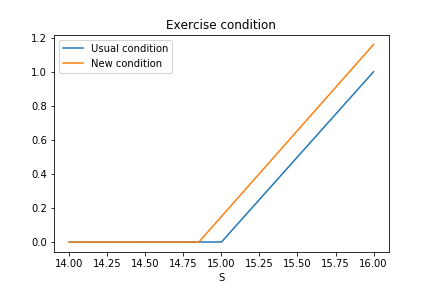
\includegraphics[scale=0.5]{payoff_comparison.png}
 % payoff_comparison.png: 0x0 pixel, 300dpi, 0.00x0.00 cm, bb=
 \caption{Comparison of exercise conditions for a European Call option with strike $K=15$, in a market with zero costs and in a market with $\theta_b=0.01$.}
 \label{fig:payoff_comparison}
\end{figure}
In the case the option is exercised, $S_T(1+ \theta_b ) > K$, the buyer pays to the writer the strike value $K$ in cash, 
and the writer delivers one share to the buyer.
In a market with transaction costs the real value (in cash) of a share incorporates the transaction costs. 
Therefore the buyer does not exercise when $S_T > K$, but when $S_T(1+ \theta_b ) > K$. 
In Figure \ref{fig:payoff_comparison} there is a comparison between the exercise conditions in a market with zero costs (as in Black-Scholes) and in a market with 
transaction costs.

The objective of the investor is to maximize the expected utility of the wealth at terminal time $T$ over all the admissible
strategies. This expectation is conditioned on the current value of cash, number of shares and value of the
stock.
The sets of trading strategies corresponding to each of the three portfolios, is obtained by using the respective wealth process inside Definition [\ref{admissible_strategies1}]. 

\begin{Definition}
 The \textbf{value function} of the maximization problem for $j=w,b,0$ is defined as:
\begin{align}\label{max_probl0}
V^j(t,b,y,s) := \sup_{\pi \in \Pi^j(t,b,y,s)} \; & \E_{t,b,y,s}\biggl[ 
            \mathcal{U}(\mathcal{W}^{j; \pi}_T) \biggr],             
\end{align}
where $\mathcal{U}: \R \to \R$ is a concave increasing utility function such that $\mathcal{U}(0)=0$.
\end{Definition}
Let us verify that the cost function is well defined. Let us consider only the case $j=0$, because for $j=w,b$ the generalization is straightforward.
\begin{Theorem}
The objective function is finite, i.e.
$$ \E_{t,b,y,s}\biggl[ \mathcal{U}(\mathcal{W}^{\pi}_T) \biggr] < \infty$$
for all $\pi \in \Pi(t,b,y,s)$.
\end{Theorem}
\begin{proof}
 Since the utility function is concave, thanks to the Jensen inequality $\E_{t,b,y,s} \bigl[\mathcal{U}(\mathcal{W}^{\pi}_T)\bigr] \leq 
 \mathcal{U}\bigl( \E_{t,b,y,s}[\mathcal{W}^{\pi}_T] \bigr)$,
 it is enough to prove $\E_{t,b,y,s}[\mathcal{W}^{\pi}_T] < \infty$.\\
 The wealth at time $T$ is:
 \begin{align*}
   \mathcal{W}^{\pi}_T &=  B^{\pi}_T + c(Y^{\pi}_T,S_T) \\
                       &\leq B^{\pi}_T + Y^{\pi}_T S_T.
 \end{align*}
 where $B^{\pi}_T$ is the solution of the first line of (\ref{DPZ_porfolio_dynamics}) i.e.
 \begin{equation*}
 B^{\pi}_T =  \frac{b}{\delta(t,T)} - \int_{t}^T
 (1+\theta_b)\frac{S_u}{\delta(u,T)} dL_u + \int_{t}^T
 (1-\theta_s) \frac{S_u}{\delta(u,T)} dM_u 
 \end{equation*}
 with $\delta(u,T) = e^{-r(T-u)}$.  
 By taking the expectation we get
 \begin{align*}
 \E_{t,b,y,s}\biggl[ \int_{t}^T (1+\theta_b)\frac{S_u}{\delta(u,T)} dL_u  \biggr] & \leq \frac{(1+\theta_b)}{\delta(t,T)} 
                                                                                    \E_{t,b,y,s}\biggl[ \biggl(\max_{u\in[t,T]} S_u \biggr)\int_{t}^T dL_u  \biggr] \\
                                                                                &\leq \frac{(1+\theta_b)}{\delta(t,T)} \E_{t,b,y,s}\biggl[ \biggl(\max_{u\in[t,T]} S_u \biggr) L_T  \biggr] 
 \end{align*}
where for simplicity we assume $L_t=0$.
Let us define the running maximum $\mathcal{M}_T := \max_{u\in[t,T]} S_{u}$. 
The term $\E \bigl[ (\mathcal{M}_T)^2 \bigr] < \infty$ because of (\ref{cond_3}).
We also know that $\E \bigl[ (L_T)^2 \bigr] < \infty $ because of the assumption (\ref{singular_moments}).
Now we can use the Schwartz inequality and obtain:
\begin{equation}
  \E_{t,b,y,s} \bigl[ \mathcal{M}_T L_T \bigr]^2  \leq \E_{t,b,y,s}[(\mathcal{M}_T)^2] \, \E_{t,b,y,s} \bigl[ (L_T)^2 \bigr] < \infty.
\end{equation}
The same argument can be applied to $\E_{t,b,y,s}\bigl[ \int_{t}^T (1-\theta_s) \frac{S_u}{\delta(u,T)} dM_u \bigr]$.\\
By using again the Schwartz inequality, we can verify that $\E_{t,b,y,s}\bigl[ Y^{\pi}_T S_T \bigr] = \E_{t,b,y,s}\bigl[ S_T(L_T - M_T) \bigr]$ is finite as well.
And this concludes the proof.
\end{proof}



The writer (buyer) option price is defined as the amount of cash to add (subtract) to the bank account, 
such that the maximal expected utility of wealth of the writer (buyer) is the same he could get with 
the zero-option portfolio.
\begin{Definition}
The writer price is the value $p^w>0$ such that 
 \begin{equation}\label{writer}
  V^0(t,b,y,s) = V^w(t,b+p^w,y,s),
 \end{equation}
 and the buyer price is the value $p^b>0$ such that
 \begin{equation}\label{buyer}
  V^0(t,b,y,s) = V^b(t,b-p^b,y,s).
 \end{equation}
\end{Definition}


\subsubsection{HJB Equation}\label{subsec_HJB}

According to the theory of stochastic optimal control presented in Chapter \ref{Chapter4},  
we can identify the DPZ model within the class of singular control problems described in Section (\ref{singular_control}).
Let us re-write the state equation (\ref{DPZ_porfolio_dynamics}) for $X^{\pi}_t = (B^{\pi}_t,Y^{\pi}_t,S_t)$ in matrix form 
\begin{align}\label{DPZ_porfolio_dynamicsM}
d X^{\pi}_t
=& 
 d \left(
\begin{array}{l}
B^{\pi}_t\\
Y^{\pi}_t\\
S_t
\end{array} \right) \\ \nonumber
  =&  \left( \begin{array}{l}
r B^{\pi}_t\\
0\\
\mu S_{t}
\end{array} \right)
dt +  \left( \begin{array}{l}
0\\
0\\
\sigma S_{t}
\end{array} \right) dW_t \\ \nonumber
&+ \underbrace{\left( \begin{array}{cc}
-S_{t}(1+\theta_b) & S_{t}(1-\theta_s) \\
1 & -1 \\
0 & 0
\end{array} \right)}_{\kappa(t,X_t)}
\underbrace{\left( \begin{array}{l}
dL_t \\
dM_t 
\end{array} \right)}_{d\xi_t},
\end{align}
which can be easily identified with the general equation (\ref{singular_SDE}).
The state $X^{\pi}_t$ takes values in $\OO$ corresponding to the solvency region $\SI$.
The objective function that we maximize in Eq. (\ref{max_probl0}) corresponds to Eq. (\ref{singular_cost_functional}) with $\hat f$ and $h$ equal to zero. 

Let us check that the Frobenius condition (\ref{Frobenius}) is satisfied.
Let us call $\tilde \theta_b = (1+\theta_b)$ and $\tilde \theta_s = (1-\theta_s)$.  The commutator is:
\begin{equation}
 \left( \begin{array}{ccc}
0 & 0 & -\tilde \theta_b \\
0 & 0 & 0 \\
0 & 0 & 0
\end{array} \right)
\left( \begin{array}{l}
 S_{t}\tilde \theta_s \\
-1 \\
0
\end{array} \right) -
 \left( \begin{array}{ccc}
0 & 0 & \tilde \theta_s \\
0 & 0 & 0 \\
0 & 0 & 0
\end{array} \right)
\left( \begin{array}{l}
-S_{t}\tilde \theta_b \\
1 \\
0
\end{array} \right) = 0
\end{equation}
which shows that the condition is satisfied.

According to singular control theory, the HJB equation of a singular control problem is a variational inequality. Here we can obtain the HJB equation of this problem 
from the general equation (\ref{variational_inequality}). We omit the subscript of $V^j$ when the discussion refers to all the three problems. 
Let us indicate $x = (b,y,s)$. Let us consider:
$$ D_x V(t,x) = \left( \frac{\partial V(t,b,y,s)}{\partial b}, \frac{\partial V(t,b,y,s)}{\partial y}, \frac{\partial V(t,b,y,s)}{\partial s} \right) $$
and
$$ \hat K := \biggl \{ \biggl( \begin{array}{c} l \\ m \end{array} \biggr) \in [0,\infty) \times [0,\infty): |l|^2 + |m|^2 = 1 \biggr \}. $$ 
Following (\ref{set_K}) we obtain
\begin{align*}
& \sup_{l,m \in \hat K}
\left( \frac{\partial V}{\partial b}, \frac{\partial V}{\partial y}, \frac{\partial V}{\partial s} \right)
\left( \begin{array}{cc}
-s(1+\theta_b) & s(1-\theta_s) \\
1 & -1 \\
0 & 0
\end{array} \right)
\left( \begin{array}{c}
l \\
m 
\end{array} \right) \\ 
= & \sup_{l,m \in \hat K}
\frac{\partial V}{\partial b} \biggl( -s(1+\theta_b)l + s(1-\theta_s)m \biggr) +
\frac{\partial V}{\partial y} \bigl( l-m \bigr) \\
= & \sup_{l,m \in \hat K}
l \biggl( -s(1+\theta_b)\frac{\partial V}{\partial b} + \frac{\partial V}{\partial y} \biggr) +
m \biggl( s(1-\theta_s)\frac{\partial V}{\partial b} - \frac{\partial V}{\partial y} \biggr)
\end{align*}

\vspace{3em}
\noindent
The terms 
$$ \biggl( -s(1+\theta_b)\frac{\partial V}{\partial b} + \frac{\partial V}{\partial y} \biggr) 
\quad \mbox{and} \quad \biggl( s(1-\theta_s)\frac{\partial V}{\partial b} - \frac{\partial V}{\partial y} \biggr)  $$
cannot be positive at the same time, otherwise we would get
$$ s(1+\theta_b)\frac{\partial V}{\partial b} < \frac{\partial V}{\partial y} < s(1-\theta_s)\frac{\partial V}{\partial b} $$
which is impossible for $s,\theta_b,\theta_s>0$. \\

\noindent
The other possibilities are 
\begin{enumerate}
 \item $\biggl(-s(1+\theta_b)\frac{\partial V}{\partial b} + \frac{\partial V}{\partial y}\biggr) > 0$ 
 and $\biggl(s(1-\theta_s)\frac{\partial V}{\partial b} - \frac{\partial V}{\partial y}\biggr) \leq 0$. \\ The optimal control is $l=1$ and $m=0$.
 \item $\biggl(-s(1+\theta_b)\frac{\partial V}{\partial b} + \frac{\partial V}{\partial y}\biggr) \leq 0$
 and $\biggl(s(1-\theta_s)\frac{\partial V}{\partial b} - \frac{\partial V}{\partial y}\biggr) > 0$. \\ The optimal control is $l=0$ and $m=1$.
 \item $\biggl(-s(1+\theta_b)\frac{\partial V}{\partial b} + \frac{\partial V}{\partial y}\biggr) < 0$ and 
 $\biggl(s(1-\theta_s)\frac{\partial V}{\partial b} - \frac{\partial V}{\partial y}\biggr) < 0$. \\ The optimal control is $l=0$ and $m=1$ or $l=1$ and $m=0$, depending on which term 
 is bigger.
\end{enumerate}

\noindent
We should also consider the case when both are zero, which happens for 
$$\frac{\partial V}{\partial b} = \frac{\partial V}{\partial y} = 0.$$ 
But this is not possible because the function $V$ is an increasing function of $b$ and $y$ 
(for a proof see Theorem 5.3.4 in \cite{Damgaard}).
Intuitively, this can be explained by thinking that an extra initial wealth provides higher final expected utility.

\noindent
From this argument we derived the optimal set $\hat K = \left( \begin{array}{c}
			   1 \\
			   0
                          \end{array} \right) \bigcup \left( \begin{array}{c}
			   0 \\
			   1
                          \end{array} \right)$.

Considering again Eq. (\ref{set_K}), together with the optimal set $\hat K$,
we obtain
$$ H \bigl(t,x, D_x V(t,x) \bigr) = \max \biggl\{ \frac{\partial V}{\partial y}-(1+\theta_b) s \frac{\partial V}{\partial b} ,
 -\bigl( \frac{\partial V}{\partial y} -(1-\theta_s)s \frac{\partial V}{\partial b} \bigr) \biggr\}. $$

\noindent 
The resulting HJB equation is
\begin{align}\label{DPZ_HJB}
& \max \; \biggl\{ \; \frac{\partial V}{\partial t} + rb\frac{\partial V}{\partial b} 
+ \mu s \frac{\partial V}{\partial s} + \frac{1}{2}\sigma^2 s^2 \frac{\partial^2 V}{\partial s^2}, \\ \nonumber
& \;  \frac{\partial V}{\partial y}-(1+\theta_b) s \frac{\partial V}{\partial b} \; 
, \; -\biggl(\frac{\partial V}{\partial y}-(1-\theta_s)s \frac{\partial V}{\partial b} \biggr) \biggr\} = 0, 
\end{align}
for $(t,b,y,s) \in [t_0,T] \times \SI$.
The terminal conditions for the three portfolio problems $j=0,w,b$ are:
\begin{equation}\label{terminal_conditions}
V^j(T,b,y,s) = \mathcal{U}\bigl( w^j(b,y,s) \bigr) \hspace{1em} \mbox{ for } \hspace{1em} (b,y,s) \in \mathcal{S}^j 
\end{equation}
with
  \begin{equation*}
   w^0(b,y,s) =  b + c(y,s).
  \end{equation*}
  \begin{equation*}
   w^w(b,y,s) =  b + c(y,s) \mathbbm{1}_{\{ s(1+\theta_b) \leq K\}} +
  \biggl( c\bigl( y-1,s \bigr) + K \biggr) \mathbbm{1}_{\{s(1+\theta_b)>K\}}.
  \end{equation*}
  \begin{equation*}
   w^b(b,y,s) = b + c(y,s) \mathbbm{1}_{\{ s(1+\theta_b) \leq K\}} +
  \biggl( c\bigl( y+1,s \bigr) - K \biggr) \mathbbm{1}_{\{s(1+\theta_b)>K\}}.
  \end{equation*}

\noindent
The variational inequality (\ref{DPZ_HJB}) says that the maximum of three operators is equal to zero.
This feature can be interpreted better if we consider the state space divided into three different regions: the \textbf{Buy}, the \textbf{Sell}
and the \textbf{No Transaction} (NT) regions.
\begin{itemize}
 \item \textbf{Buy}
  \begin{equation*}
   \begin{cases}
     & \frac{\partial V}{\partial t} + rb\frac{\partial V}{\partial b} + \mu s \frac{\partial V}{\partial s} + \frac{1}{2}\sigma^2 s^2 \frac{\partial^2 V}{\partial s^2} \leq 0\\ 
     & \frac{\partial V}{\partial y}-(1+\theta_b) s \frac{\partial V}{\partial b} = 0 \\
     & -\biggl(\frac{\partial V}{\partial y}-(1-\theta_s)s \frac{\partial V}{\partial b} \biggr) \leq 0.
   \end{cases}
  \end{equation*}
 \item \textbf{Sell}
  \begin{equation*}
   \begin{cases}
     & \frac{\partial V}{\partial t} + rb\frac{\partial V}{\partial b} + \mu s \frac{\partial V}{\partial s} + \frac{1}{2}\sigma^2 s^2 \frac{\partial^2 V}{\partial s^2} \leq 0 \\ 
     & \frac{\partial V}{\partial y}-(1+\theta_b) s \frac{\partial V}{\partial b} \leq 0 \\
     & -\biggl(\frac{\partial V}{\partial y}-(1-\theta_s)s \frac{\partial V}{\partial b} \biggr) = 0.
   \end{cases}
  \end{equation*}
 \item \textbf{No Transaction}
  \begin{equation*}
   \begin{cases}
     & \frac{\partial V}{\partial t} + rb\frac{\partial V}{\partial b} + \mu s \frac{\partial V}{\partial s} + \frac{1}{2}\sigma^2 s^2 \frac{\partial^2 V}{\partial s^2} = 0 \\ 
     & \frac{\partial V}{\partial y}-(1+\theta_b) s \frac{\partial V}{\partial b} \leq 0 \\
     & -\biggl(\frac{\partial V}{\partial y}-(1-\theta_s)s \frac{\partial V}{\partial b} \biggr) \leq 0.
   \end{cases}
  \end{equation*}
\end{itemize}
The optimization problem is a free boundary problem, and its solution consists in finding the value function $V$ and the 
optimal boundaries that divide the three regions.
The Buy and Sell regions do not intersect, and are separated by the NT region. 
In the derivation of the optimal set $\hat K$, we have seen that it is not optimal to buy and sell a share at the same time. 
This is reasonable since buying and selling a share at the same time just decreases the 
total wealth, because of the transaction costs, and therefore makes no sense. 

The free boundaries of the NT region completely characterize the investor's trading strategy.
The optimal strategy consists in keeping the portfolio process inside the NT region. 
If the portfolio exits the NT region, the optimal strategy is to trade in order to bring it back to the NT region.

In the Buy and Sell regions the value functions is constant along the directions of the trades.
We get respectively:
\begin{itemize}
 \item[Buy]: \hspace{2em} $V(t,b,y,s) = V(t,b-s(1+\theta_b)\Delta L_t,y+\Delta L_t,s).$
 \item[Sell]: \hspace{2em} $ V(t,b,y,s) = V(t,b+s(1-\theta_s)\Delta M_t,y-\Delta M_t,s).$
\end{itemize}
where $\Delta L_t$ and $\Delta M_t$ are the number of shares respectively bought or sold in the trade.
%In the NT region the portfolio evolves according to the portfolio equation (\ref{DPZ_porfolio_dynamics}), with $dL=dM=0$.
%It means that the number of shares remains constant as long as the portfolio stays in the NT region.





\subsection{DPZ with jumps}\label{DPZ_j_sec}


The purpose of this thesis is to extend the DPZ model in order to include jumps in the stock dynamics. 
Following the framework of \cite{Kab16} let us introduce a market model with proportional transaction costs 
that consider an exponential Lévy process for the stock dynamics, as in \ref{exp_sde2}.
The state of the portfolio at time $t\in [t_0,T]$ is $(B^{\pi}_t,Y^{\pi}_t,S_t)$ and evolves following the SDE:
\begin{equation}\label{porfolio_dynamics}
 \begin{cases}
 dB^{\pi}_t &=  rB^{\pi}_t dt - (1+\theta_b)S_{t^-} dL_t + (1-\theta_s) S_{t^-} dM_t \\
 dY^{\pi}_t &=  dL_t - dM_t \\
 dS_t &=  S_{t^-} \left( \mu dt + \sigma dW_t + \int_{\R} (e^z-1) \tilde N(dt,dz) \right).
\end{cases}
\end{equation}
The strategy $\{\pi_t\}_{t \in [t_0,T]}$ is a cádlág, $\mathcal{F}_t$-predictable\footnote{We are considering the Wiener-Poisson filtration 
defined in Section \ref{Optimal_control_framework}.}, nondecreasing process with bounded variation, such that
$ \pi_{t_0^-} = \bigl ( L_{t_0^-} , M_{t_0^-} \bigr ) = (0,0)$. 
Under these assumptions the portfolio process 
$\bigl \{(B^{\pi}_t,Y^{\pi}_t,S_t)\bigr \}_{t \in [t_0,T]}$ has a cádlág modification, and this is what we consider.

If at time $t$ there is an unpredictable jump in the stock price $\Delta S_t = S_t - S_{t^-}$, a possible transaction should happen after the jump.
The control process $\{\pi_t\}_{t \in [t_0,T]}$ is assumed to be predictable, i.e. measurable with respect to the left-continuous filtration $\{\mathcal{F}_{t^-}\}_{t \in [t_0,T]}$.
Therefore, a jump in the price and a jump in the control cannot occur simultaneously, almost surely. 
A deeper digression on this topic can be found in Section 2 of \cite{Kab16}.   
If the investor at time $t$ observes a jump in the price and decides to rebalance his portfolio, he will trade at some time $u>t$ at the price $S_{u^-}$. 
Under this framework, as explained in \cite{Kab16}, the optimal strategy cannot exist. 

The definitions of cash value (\ref{cost_function}), of total wealth (\ref{wealth_process}), (\ref{wealth_buyer}), (\ref{wealth_writer}) and the solvency regions
(\ref{solvency_region}) are kept the same. The set of admissible trading strategy will be changed.

Since the underlying stock follows a process with jumps, it is not guaranteed that the portfolio stays
solvent for all $t \in [t_0,T]$. When holding short positions, it is possible that a sudden increase in the stock price 
causes the total wealth to jump out of the solvency region. 
The same can happen with a downward jump when the investor is long in stocks and negative in cash. 
The immediate decrease of the stock's price makes him unable to pay the debts.
\begin{Definition}
The first \textbf{exit time} from the solvency region is defined as:
\begin{equation}\label{exit_time}
 \tau := \inf \bigl\{ t \in [t_0,T] : (B^\pi_t,Y^\pi_t,S_t) \not\in \SI \bigr\}.
\end{equation} 
\end{Definition}
\begin{Definition}\label{set_trad_strat}
The set of \textbf{admissible trading strategies} $\Pi(t_0,b,y,s)$   
is the set of all cádlág, nondecreasing, predictable, bounded variation processes $\{\pi_t\}_{t \in [t_0,T]}$
such that $(B^\pi_t,Y^\pi_t,S_t)$ is a solution of (\ref{porfolio_dynamics}) with initial values $(B^\pi_{t_0} = b, Y^\pi_{t_0} = y, S_{t_0} = s)$ and such that
$\pi_t = \pi_{\tau}$ for all $t \geq \tau$.  
\end{Definition}

The objective of the investor is to maximize the expected utility of the wealth at $\tau^j \wedge T$ over all the admissible
strategies. This expectation is conditioned on the current value of cash, number of shares and value of the
stock.
\begin{Definition}
 The \textbf{value function} of the maximization problem for $j=w,b,0$ is defined as:
\begin{align}\label{max_probl1}
V^j(t,b,y,s) := \sup_{\pi \in \Pi^j(t,b,y,s)} \; & \E_{t,b,y,s}\biggl[ 
            \mathcal{U}(\mathcal{W}^{j; \pi}_T) \; \mathbbm{1}_{\{\tau^j > T\}} \\ \nonumber
             &+ e^{ \beta (T-\tau^j)} \mathcal{U}( \mathcal{W}^{j; \pi}_{\tau^j} ) \; 
             \mathbbm{1}_{\{\tau^j \leq T\}}\biggr],             
\end{align}
where $\mathcal{U}: \R \to \R$ is a concave increasing utility function such that $\mathcal{U}(0)=0$, and $\beta \geq 0$.
\end{Definition}

The HJB equation associated to this stochastic control problem is obtained following the same steps we used to derive (\ref{DPZ_HJB}). The infinitesimal generator of the price 
dynamics has the 
form (\ref{inf_gen_exp_levy}) for exponential Lévy processes. The HJB variational inequality is
\begin{align}\label{HJB1}
& \max \; \biggl\{ \; \frac{\partial V^j}{\partial t} + rb\frac{\partial V^j}{\partial b} 
+ \mu s \frac{\partial V^j}{\partial s} + \frac{1}{2}\sigma^2 s^2 \frac{\partial^2 V^j}{\partial s^2} \\ \nonumber
&+ \int_\mathbb{R}
\biggl[ V^j(t,b,y,se^z) - V^j(t,b,y,s) - s(e^z-1)\frac{\partial V^j}{\partial s} \biggr] \nu(dz) \;,\\ \nonumber
& \;  \frac{\partial V^j}{\partial y}-(1+\theta_b) s \frac{\partial V^j}{\partial b} \; 
, \; -\biggl(\frac{\partial V^j}{\partial y}-(1-\theta_s)s \frac{\partial V^j}{\partial b} \biggr) \biggr\} = 0, 
 \end{align}
for $(t,b,y,s) \in [t_0,T) \times \SI^j$ and $j=0,w,b$.   
The terminal boundary conditions are given by Eq. (\ref{terminal_conditions}).
Since this HJB equation is a PIDE,
the non-local integral operator implies to 
define the lateral conditions not only on the boundary
of the solvency region, but also beyond:
\begin{equation}\label{lat_bound}
V^j(t,b,y,s) = e^{ \beta (T-t)} \mathcal{U}\bigl( b + c(y,s)\bigr) 
\end{equation}
for $t \in [t_0,T)$ , $(b,y,s) \not \in \mathcal{S}$ and for $j=0,w,b$. 


\subsection{Variable reduction}\label{variable_reduction}


In the DPZ model introduced in Section \ref{DPZ_sec}, the portfolio is solvent for every
$t \in [t_0,T]$ and it is always possible to calculate the utility 
of the wealth at the terminal time $\mathcal{U}(\mathcal{W}^{\pi}_T)$.
In the extended model of Section \ref{DPZ_j_sec} the stock process can jump, and in presence of short positions the portfolio can go bankrupt at any time before the maturity $T$. 

With the intention of simplifying the maximization problem (\ref{max_probl1}) and reducing the number of variables, 
%we restrict our attention to the subset of solvent paths. 
we restrict our attention to the case of no bankruptcy.
A possible idea is to consider a positive initial wealth, and define the restricted set of admissible strategies as the set of $\{\pi_t\}_{t \in [t_0,T]}$ such that 
$B^{\pi}_t \geq 0$ and $Y^{\pi}_t \geq 0$ for all $t\in [t_0,T]$ (see \cite{Benth02}).
However, in order to implement a hedging strategy, we are interested in portfolios containing short positions as well.
So, we can assume that the investor has a very large credit availability $C$ in the sense that
\begin{equation}\label{P_tau}
 \PP(\tau > T) \underset{C\to \infty}{\to} 1.
\end{equation}
In practical terms, we ignore the possibility of default. The solvency region becomes $\mathcal{S} = \R^2 \times \R^{+}$ and no lateral boundary conditions are imposed.

As in \cite{DaPaZa93}, for $\gamma>0$, we consider the exponential utility function
\begin{equation}\label{exp_util}
 \mathcal{U}(x) := 1- e^{-\gamma x}.
\end{equation}
Thanks to (\ref{P_tau}) and (\ref{exp_util}) we can remove $\{B^{\pi}_t\}_{t \in [t_0,T]}$ from the state dynamics.
By solving (\ref{porfolio_dynamics}) we get
\begin{equation}\label{BT}
B^{\pi}_T =  \frac{B^{\pi}_{t}}{\delta(t,T)} - \int_{t}^T
(1+\theta_b)\frac{S_u}{\delta(u,T)} dL_u + \int_{t}^T
 (1-\theta_s) \frac{S_u}{\delta(u,T)} dM_u 
\end{equation}
where $\delta(u,T) = e^{-r(T-u)}$.
Using together (\ref{P_tau}), (\ref{exp_util}) and (\ref{BT}), and the wealth processes (\ref{wealth_process}),(\ref{wealth_writer}),(\ref{wealth_buyer}), 
we obtain for $B^\pi_{t} = b$, $Y^\pi_{t} = y$, $S_{t} = s$ and $j=0,w,b$:
\begin{align}\label{var_reduct}
   V^j(t,b,y,s) = \sup_{\pi} \; \E_{t,b,y,s}\biggl[  1- e^{-\gamma \mathcal{W}^j(T) } \biggr]  % \\ \nonumber 
	     = 1- e^{-\gamma \frac{b}{\delta(t,T)}} Q^j(t,y,s),
\end{align} 
where
\begin{align}\label{minimization}
Q^j(t,y,s) = \inf_{\pi} \; \mathbb{E}_{t,y,s}\biggl[ \; &
	     e^{-\gamma \bigl[ -\int_{t}^T (1+\theta_b) \frac{S_u}{\delta(u,T)} dL_u +
	     \int_{t}^T (1-\theta_s) \frac{S_u}{\delta(u,T)} dM_u \bigr] } \, \\ \nonumber 
	     & \times H^j(Y^{\pi}_T,S_T) \bigg]  
\end{align}
is our new minimization problem.
The exponential term inside the expectation can be considered as a discount factor, and the second term 
$H^j(y,s) = Q^j(T,y,s)$ is the terminal payoff:
\begin{itemize}
 \item No option:
 \begin{equation}\label{terminal_c}
  H^0(y,s) = e^{-\gamma \, c(y,s)}.
 \end{equation}
 \item Writer:
  \begin{equation}\label{terminal_w}
  H^w(y,s) = e^{-\gamma \bigl[ c(y,s)\mathbbm{1}_{\{s(1+\theta_b) \leq K\}} + 
 \bigl( c( y-1,s) + K \bigr) \mathbbm{1}_{\{s(1+\theta_b)>K\}} \bigr] }.
 \end{equation}
 \item Buyer:
  \begin{equation}\label{terminal_b}
  H^b(y,s) = e^{-\gamma \bigl[ c(y,s)\mathbbm{1}_{\{s(1+\theta_b) \leq K\}} + 
 \bigl( c( y+1,s) - K \bigr) \mathbbm{1}_{\{s(1+\theta_b)>K\}} \bigr] }.
 \end{equation}
\end{itemize}
Using conditions (\ref{writer}), (\ref{buyer}) together with (\ref{var_reduct}), we obtain the explicit formulas for the option prices:
\begin{equation}\label{opt_w}
 p^w(t_0,y,s) = \frac{\delta(t_0,T)}{\gamma} \log \biggl( \frac{Q^w(t_0,y,s)}{Q^0(t_0,y,s)} \biggr),
\end{equation}
\begin{equation}\label{opt_b}
 p^b(t_0,y,s) = \frac{\delta(t_0,T)}{\gamma} \log \biggl( \frac{Q^0(t_0,y,s)}{Q^b(t_0,y,s)} \biggr).
\end{equation}

Since $Q^j(t,y,s)$ is independent on $b$, let us write
$ Q^j(t,y,s) := 1 - V^j(t,0,y,s)$.
It is convenient to pass to the log-variable $x = \log(s)$, such that
\begin{equation}\label{log_var}
s \frac{\partial}{\partial s} = \frac{\partial}{\partial x}, \hspace{2em} 
s^2 \frac{\partial^2}{\partial s^2} = \frac{\partial^2}{\partial x^2} - \frac{\partial}{\partial x} . 
\end{equation}
For $j=0,w,b$, the HJB Eq. (\ref{HJB1}) becomes:
\begin{align}\label{HJB2}
& \min \; \biggl\{ \; \frac{\partial Q^j}{\partial t} + (\mu-\frac{1}{2}\sigma^2) \frac{\partial Q^j}{\partial x}
+ \frac{1}{2}\sigma^2 \frac{\partial^2 Q^j}{\partial x^2} \\ \nonumber
&+ \int_\mathbb{R}
\biggl[ Q^j(t,y,x+z) - Q^j(t,y,x) - (e^z-1)\frac{\partial Q^j}{\partial x} \biggr] \nu(dz) \;,  \\ \nonumber
& \; \frac{\partial Q^j}{\partial y} +(1+\theta_b) e^x \frac{\gamma}{\delta(t,T)}Q^j \; , 
\; -\biggl( \frac{\partial Q^j}{\partial y}+(1-\theta_s)e^x \frac{\gamma}{\delta(t,T)} Q^j 
\biggr) \biggr\} = 0. 
 \end{align}
% This equation is well defined for $Q^j \in C^{1,1,2}\bigl( (t_0,T) \times \R^2\bigr) \bigcap C_2\bigl( [t_0,T] \times \R^2 \bigr) $. 








\section{Existence of viscosity solution}\label{Existence_viscosity}

The general fact that value functions of control problems can be characterized as
viscosity solutions of certain partial differential equations is a direct consequence of the dynamic
programming principle. For singular control problems, however, the classical approach of \cite{PLL83}
fails because the state process may jump due to the singular control and it needs thus not stay
in a small ball\footnote{For processes of type (\ref{singular_SDE}) it is not possible to apply the theorem (\ref{stochastic_theorem}).} 
for a small $\Delta t$.
This problem can be circumvented by relying on the
existence of the optimal control, as done in \cite{DaPaZa93}. However, in our proof we will not assume the existence of the optimal control, because 
in this framework it does not exist (as explained in Section \ref{DPZ_j_sec} it is not possible to give an immediate response at the jump time of the stock).
We will assume that the \textbf{DPP} for the singular control problem (\ref{porfolio_dynamics}), (\ref{max_probl1}) holds, and that the value function  
is continuous. We refer to Sections 4 and 9 of \cite{Kab16} for the proofs of these statements. 

In this section we prove that the value function (\ref{max_probl1}), can be interpreted 
as the viscosity solution of the HJB equation (\ref{HJB1}).
%The proof follows the approach in \cite{OkSu01}.

Let us call $\tau_{\SI}$ the first exit time from $\SI$.
Since the stock dynamics is stochastically continuous and the control process $\pi$ cannot be the cause of bankruptcy,
we can exclude an immediate jump out of the solvency region, i.e. $\PP ( \tau_{\SI} = t_0 ) =0$.

We have to interpret the HJB equation (\ref{HJB1}) with boundary conditions (\ref{lat_bound}) and (\ref{terminal_conditions}) 
as a parabolic problem of the type (\ref{parabolic_PIDE}). 
Let us use the notation $x = (b,y,s)$ to indicate a point in $\R^2\times \R^+$. In order to satisfy the parabolic conditions we reformulate the HJB as 
\begin{align}\label{HJB22}
& \min \; \biggl\{ - \biggl( \; \frac{\partial V}{\partial t} + rb\frac{\partial V}{\partial b} 
+ \mu s \frac{\partial V}{\partial s} + \frac{1}{2}\sigma^2 s^2 \frac{\partial^2 V}{\partial s^2} \\ \nonumber
&+ \int_\mathbb{R}
\biggl[ V(t,b,y,se^z) - V(t,b,y,s) - s(e^z-1)\frac{\partial V}{\partial s} \biggr] \nu(dz) \; \biggr) ,\\ \nonumber
& \; - \biggl( \frac{\partial V}{\partial y}-(1+\theta_b) s \frac{\partial V}{\partial b} \biggr) \; 
, \; + \biggl(\frac{\partial V}{\partial y}-(1-\theta_s)s \frac{\partial V}{\partial b} \biggr) \biggr\} = 0. 
\end{align}
We indicate this function with
$ F(t,x,V,D_t V,D_{x} V,D_{xx}V,\I(t,x,V)) = 0$ in the domain $(t,x) \in [t_0,T) \times \SI$.
To simplify the notation, let us introduce the integro-differential infinitesimal generator:
\begin{align*}
 \LL V(t,x) &:= -\biggl( \frac{\partial V}{\partial t}(t,x) + rb\frac{\partial V}{\partial b}(t,x) 
  + \mu s \frac{\partial V}{\partial s}(t,x) + \frac{1}{2}\sigma^2 s^2 \frac{\partial^2V}{\partial s^2}(t,x)\biggr) \\
  &- \int_{\R}
\biggl[ V(t,b,y,se^z) - V(t,b,y,s) - s(e^z-1)\frac{\partial V}{\partial s} \biggr] \nu(dz),
\end{align*}
such that the equation (\ref{HJB22}) has the form
\begin{equation}\label{qvi_min}
  \min \; \biggl\{ \; \LL V(t,x),
  \, -(V_y-(1+\theta_b)sV_b) \, , \; V_y-(1-\theta_s)s V_b \biggr\} = 0.
\end{equation}
In order to prove that $V(t,x)$ is a viscosity solution we need to verify both the subsolution and supersolution properties.



\subsection{Subsolution}

In this section we prove that the value function can be interpreted as a viscosity subsolution of the HJB equation associated to the maximization problem. 
We enunciate the following theorem:
\begin{Theorem}\label{subsolution_th}
 The value function of the maximization problem (\ref{max_probl1}), is a viscosity subsolution of the Eq. (\ref{qvi_min}).
\end{Theorem}
\begin{proof}
Let us consider a test function $ \phi \in C^2([t_0,T] \times \R^2\times \R^+) \bigcap \mathcal{C}_2([t_0,T] \times \R^2\times \R^+)$ such that 
$(\bar t,\bar x) \in [t_0,T] \times \SI$ is a maximum point for $V-\phi$:
\begin{equation}
 V(\bar t,\bar x) - \phi(\bar t,\bar x) \geq V(t,x) - \phi(t, x) \hspace{2em} \forall (t,x) \in [t_0,T] \times \SI
\end{equation}
and we assume without loss of generality that:
\begin{equation}\label{max_point}
V(\bar t,\bar x) = \phi(\bar t,\bar x)  
\end{equation}
so we can write:
\begin{equation}\label{max_point2}
V(t,x) \leq \phi(t, x) 
\end{equation}
We want to prove that
$$ F(\bar t,\bar x,V(\bar t, \bar x),D_t \phi(\bar t, \bar x),D_x \phi(\bar t, \bar x),D_{xx}\phi(\bar t, \bar x),
\I(\bar t, \bar x,\phi(\bar t, \bar x))) \leq 0  $$
\textbf{Reductio ad absurdum:}\\
Let us assume that 
$$F(\bar t,\bar x,V(\bar t, \bar x),D_t \phi(\bar t, \bar x),D_x \phi(\bar t, \bar x),D_{xx}\phi(\bar t, \bar x),
\I(\bar t,\bar x,\phi(\bar t, \bar x))) >0.$$ 
This means that all the terms inside the minimum in Eq. (\ref{qvi_min}) are positive, i.e. exists $\kappa >0$ such that:
\begin{enumerate}
 \item $ \LL \phi(\bar t, \bar x) > \kappa ,$
 \item $-\left(\frac{\partial \phi}{\partial y}(\bar t, \bar x)
 -(1+\theta_b) \bar s \frac{\partial \phi}{\partial b}(\bar t, \bar x)\right) > \kappa,$
 \item $\frac{\partial \phi}{\partial y}(\bar t, \bar x)-(1-\theta_s) \bar s \frac{\partial \phi}{\partial b}(\bar t, \bar x) > \kappa.$
\end{enumerate}
Since the test function is smooth by definition, there exists a closed ball $\mathcal{B}(\bar x, \rho) \subset \SI$
where the three previous conditions are satisfied $\forall x \in \mathcal{B}(\bar x, \rho)$. 
We can define the exit time of the process $\{X^{\pi}_t\}_{t \in [\bar t, T\wedge \tau_{\SI}]}$, with $X^{\pi}_{\bar t} = \bar x$, from the ball $\mathcal{B}(\bar x, \rho)$ as
\begin{equation}
 \tau_{\rho} := \inf \{ t \in [\bar t,T] : X^{\pi}_t \not \in \mathcal{B}(\bar x, \rho) \} \wedge T^{\rho},
\end{equation}
with $T^{\rho}>0$.
Since $\mathcal{B}(\bar x, \rho) \subset \SI$ it follows that $\PP( \tau_{\rho} \leq \tau_{\SI}) =1$.\\
We want to localize the problem, inside the ball $\mathcal{B}(\bar x, \rho) $ where the three conditions above are satisfied.
For this purpose, let us define the ball $\mathcal{B}(\bar x, \delta) \subset \mathcal{B}(\bar x, \rho) $ for $\delta < \rho$,
and the exit time
\begin{equation}\label{tau_delta0}
 \tau_{\delta} := \inf \{ t \in [\bar t,T] : X^{\pi}_t \not \in \mathcal{B}(\bar x, \delta) \} \wedge T^{\delta},
\end{equation}
with $T^{\delta} < T^{\rho}$.   
It follows that $\PP(\tau_{\delta} \leq \tau_{\rho}) = 1$. \\
It is reasonable to assume that $| T^{\delta}-\bar t | = C \delta^k$, for some $C,k>0$.

Let us denote with $t_k$ the jump times of $\{\pi_t\}_{t \in [\bar t, \tau_{\delta}]}$ and indicate the continuous parts of $\pi$ as 
$\pi^c = (L^c, M^c)$ with
\begin{equation}
 L^c_t = L_t - \sum_{\bar t \leq t_k \leq \tau_{\delta}} \Delta L_{t_k} \quad \mbox{ and } \quad  M^c_t = M_t - \sum_{\bar t \leq t_k \leq \tau_{\delta}} \Delta M_{t_k}.
\end{equation}
The state process $X^{\pi}$ may exit from $ \mathcal{B}(\bar x, \rho) $ or because of
the uncontrolled portfolio dynamics or due to the action of the control.

In order to prevent the exit due to the uncontrolled dynamics, we can take advantage from the stochastic continuity property of the stock process $S$. 
For this purpose, we can 
consider the evolution of the portfolio $X^{\pi=0}$ (subject to a null control), up to the exit time from the ball $ \mathcal{B}(\bar x, \delta) $. 
Let us indicate with $\tau_{\delta,0}$ the exit time of $X^{\pi=0}$ from $ \mathcal{B}(\bar x, \delta) $:
\begin{equation}\label{tau_delta}
 \tau_{\delta,0} := \inf \{ t \in [t_0,T] : X^{\pi=0}_t \not \in \mathcal{B}(\bar x, \delta) \} \wedge T^{\delta}.
\end{equation}
Thanks to Theorem \ref{stochastic_theorem}, Eq. (\ref{cond_2}) and using $\tau_{\delta,0} \in [\bar t, T^{\delta}]$, for $K>0$ we have that 
$$\PP(\tau_{\delta,0} = \tau_{\rho}) = 
\PP( |X^{\pi=0}_{\tau_{\delta,0}} - \bar x| \geq \rho ) \leq \frac{K}{\rho} \sqrt{T^{\delta} - \bar t} \leq \frac{K\,C}{\rho}\delta^{\frac{k}{2}} . $$ 
Therefore we can select the values of $\delta$ such that the probability that $X^{\pi=0}_{\tau_{\delta,0}}$ is not included in $ \mathcal{B}(\bar x, \rho) $ 
can be made arbitrarily small.
In Theorem (\ref{ball_theorem}) below, we prove that when the 
control is not the cause of the exit form $\mathcal{B}(\bar x, \delta)$,  
the controlled process $X^{\pi}_{\tau_{\delta}}$ is close to $X^{\pi=0}_{\tau_{\delta,0}}$ for a small enough $\delta$. 
It follows that the exit probability of $X^{\pi}_{\tau_{\delta}}$ from   
$\mathcal{B}(\bar x, \rho)$ can again be made arbitrarily small.

On the other hand, in order to prevent the exit due to a jump in $\pi$ we can take advantage from the linearity of the control terms in Eq. (\ref{DPZ_porfolio_dynamics}). 
In other words, any transaction can be split into two or more simultaneous smaller transactions.
We will only consider the fraction of the control jump such that the process does not exit from $\mathcal{B}(\bar x, \delta)$. 
In the following, in order to get a more readable notation, when necessary we indicate $X_t$ with $X(t)$.
Let us define the fraction
\begin{align}\label{c_bar}
 \tilde \alpha :=& \inf \biggl\{ \alpha \in [0,1] \, : \\ \nonumber
 & X^{\pi}(\tau_{\delta}^-) + \biggl( - (1+\theta_b) S(\tau_{\delta}^-)\, \alpha  \Delta L_{\tau_{\delta}} 
 + (1-\theta_s) S(\tau_{\delta}^-)\, \alpha \Delta M_{\tau_{\delta}}, \; \\ \nonumber
 & \alpha \Delta L_{\tau_{\delta}} - \alpha \Delta M_{\tau_{\delta}}, \; 0 \biggr)
 \not \in \mathcal{B}(\bar x, \delta) \biggr\}. 
\end{align}
and the control process $ \tilde \pi_t = (\tilde L_t, \tilde M_t)$ defined for $t \in [\bar t, \tau_{\delta}]$, such that
\begin{equation}
 \tilde \pi^c := \pi^c \quad \mbox{and} \quad
 \Delta \tilde \pi_t := \begin{cases}
                      \Delta \pi_t \quad &\mbox{if} \quad t = t_k \\
                      \tilde \alpha \Delta \pi_t \quad &\mbox{if} \quad t = \tau_{\delta}.  
                     \end{cases}
\end{equation}
It follows that the state process satisfies $X^{\pi}_t = X^{\tilde \pi}_t$ for $t \in [\bar t, \tau_{\delta} )$ and 
\begin{align*}
 X^{\pi}_{\tau_{\delta}} =\, X^{\tilde \pi}_{\tau_{\delta}} \, +& \, \biggl( (1-\tilde \alpha) \bigl[ - (1+\theta_b) S(\tau_{\delta}^-)\, \Delta L_{\tau_{\delta}} 
 + (1-\theta_s) S(\tau_{\delta}^-)\, \Delta M_{\tau_{\delta}} \bigr] , \; \\ \nonumber
& (1-\tilde \alpha) \bigl[ \Delta L_{\tau_{\delta}} - \Delta M_{\tau_{\delta}} \bigr], \; 0 \biggr). 
\end{align*}
At time $\tau_{\delta}$ the process $X^{\pi}_{\tau_{\delta}} \not \in \mathcal{B}(\bar x, \delta)$, while $X^{\tilde \pi}_{\tau_{\delta}} \in \partial \mathcal{B}(\bar x, \delta)$. 


By the DPP (\ref{DPP22}), for every $\epsilon > 0$, there exists an an $\epsilon$-optimal control $\pi \in \Pi(\bar t,\bar x)$ such that
\begin{align}
  V(\bar t, \bar x) & \leq \E_{\bar t, \bar x} \Bigl[ V(\tau_{\delta}, X^{\pi}_{\tau_{\delta}}) \Bigr] +\epsilon \\ \nonumber
                    &= \E_{\bar t, \bar x} \Biggl[ \E_{\tau_{\delta}, X^{\tilde \pi}_{\tau_{\delta}}} \bigl[ V(\tau_{\delta}, X^{\pi}_{\tau_{\delta}}) \bigr] \Biggr] +\epsilon \\ \nonumber
                    &= \E_{\bar t, \bar x} \Bigl[ V(\tau_{\delta}, X^{\tilde \pi}_{\tau_{\delta}}) \Bigr] +\epsilon,
\end{align}
where in the second line we used the iterated conditional expectation property.
Using (\ref{max_point}) and (\ref{max_point2}) we can write:
\begin{equation*}
 \phi(\bar t, \bar x) = V(\bar t, \bar x) \; \leq \E_{\bar t, \bar x}[V(\tau_{\delta}, X^{\tilde \pi}_{\tau_{\delta}})] + \epsilon \; 
 \leq \E_{\bar t, \bar x}[\phi(\tau_{\delta}, X^{\tilde \pi}_{\tau_{\delta}})] + \epsilon.
\end{equation*}
Since the test function $\phi$ is smooth, we can use the generalized It\=o formula (see Appendix A in \cite{OkSu01}).
\begin{align}\label{first_inequality}
 0 \; \leq & \; \E_{\bar t, \bar x} \biggl[ \phi(\tau_{\delta}, X^{\tilde \pi}_{\tau_{\delta}}) - \phi(\bar t, \bar x) \biggr] + \epsilon \\ \nonumber
    = & \; \E_{\bar t, \bar x} \biggl[ \int_{\bar t}^{\tau_{\delta}} -\LL \phi(t,X^{\tilde \pi}_t) dt \\ \nonumber
    & + \int_{\bar t}^{\tau_{\delta}} \left(\frac{\partial \phi}{\partial y}(t, X^{\tilde \pi}_t) -(1+\theta_b) S_{t^-} \frac{\partial \phi}{\partial b}( t, X^{\tilde \pi}_t)\right) dL^c_t \\ \nonumber
    & - \int_{\bar t}^{\tau_{\delta}} \left(\frac{\partial \phi}{\partial y}( t, X^{\tilde \pi}_t)-(1-\theta_s) S_{t^-} \frac{\partial \phi}{\partial b}( t, X^{\tilde \pi}_t)\right) dM^c_t \\ \nonumber
    & + \sum_{\bar t \leq t_k \leq \tau_{\delta}} \biggl( \phi \bigl( t_k, B^{\tilde \pi}(t_k^-) - (1+\theta_b) S(t_k^-)\, \Delta \tilde L_{t_k}, Y^{\tilde \pi}(t_k^-) 
      + \Delta \tilde L_{t_k}, S(t_k) \bigr) \\ \nonumber 
    & \hspace{4em} - \phi \bigl(t_k, B^{\tilde \pi}(t_k^-), Y^{\tilde \pi}(t_k^-), S(t_k) \bigr) \biggr) \\ \nonumber
    & + \sum_{\bar t \leq t_k \leq \tau_{\delta}} \biggl( \phi \bigl( t_k, B^{\tilde \pi}(t_k^-) + (1-\theta_s) S(t_k^-)\, \Delta \tilde M_{t_k}, Y^{\tilde \pi}(t_k^-) 
      - \Delta \tilde M_{t_k}, S(t_k) \bigr) \\ \nonumber
    & \hspace{4em} - \phi \bigl(t_k, B^{\tilde \pi}(t_k^-), Y^{\tilde \pi}(t_k^-), S(t_k) \bigr) \biggr) \biggr] + \epsilon
\end{align}
where the expectation of the martingale terms is zero\footnote{
The martingale terms have the same expression as (\ref{term1}) and (\ref{term2}). 
Thanks to the smoothness assumption of $\phi$, the derivatives of $\phi$ are continuous in $[\bar t, \tau_{\delta}] \times \mathcal{B}(\bar x, \delta)$ and therefore are bounded.
Using the same arguments as in Theorem \ref{Theorem_PIDE} it follows that the expectations are zero. }. 
Let us express the terms in the sums in an integral form. We obtain
\begin{align}\label{second_inequality}
 0 \; \leq & \; \E_{\bar t, \bar x} \biggl[ \int_{\bar t}^{\tau_{\delta}} -\LL \phi(t,X^{\tilde \pi}_t) dt \\ \nonumber
    & + \int_{\bar t}^{\tau_{\delta}} \left(\frac{\partial \phi}{\partial y}(t, X^{\tilde \pi}_t) -(1+\theta_b) S_{t^-} \frac{\partial \phi}{\partial b}( t, X^{\tilde \pi}_t)\right) dL^c_t \\ \nonumber
    & - \int_{\bar t}^{\tau_{\delta}} \left(\frac{\partial \phi}{\partial y}( t, X^{\tilde \pi}_t)-(1-\theta_s) S_{t^-} \frac{\partial \phi}{\partial b}( t, X^{\tilde \pi}_t)\right) dM^c_t \\ \nonumber
    & + \sum_{\bar t \leq t_k \leq \tau_{\delta}} \int_{0}^{\Delta \tilde L_{t_k}} \left(\frac{\partial \phi}{\partial y}(t_k, X^{\tilde \pi}_{t_k}) -(1+\theta_b) S(t_k^-) 
                  \frac{\partial \phi}{\partial b}( t_k, X^{\tilde \pi}_{t_k})\right) dL \\ \nonumber 
    & + \sum_{\bar t \leq t_k \leq \tau_{\delta}} \int_{0}^{\Delta \tilde M_{t_k}} \left(-\frac{\partial \phi}{\partial y}( t_k, X^{\tilde \pi}_{t_k})+(1-\theta_s) S(t_k^-) 
      \frac{\partial \phi}{\partial b}( t_k, X^{\tilde \pi}_{t_k})\right) dM \biggr] + \epsilon \\ \nonumber
  < & -\kappa \biggl( \E_{\bar t, \bar x} \bigl[ \tau_{\delta} - \bar t \bigr] + \E_{\bar t, \bar x} \bigl[ L^c_{\tau_{\delta}} - L^c_{\bar t} \bigr]  
    + \E_{\bar t, \bar x} \bigl[ M^c_{\tau_{\delta}}-M^c_{\bar t} \bigr] \\ \nonumber 
    & + \sum_{\bar t \leq t_k \leq \tau_{\delta}}  \E_{\bar t, \bar x} \bigl[ \Delta \tilde L_{t_k} + \Delta \tilde M_{t_k} \bigr]   \biggr) + \epsilon \\ \nonumber
    \underset{\epsilon \to 0}{<} & \quad 0.   
\end{align}
Let us recall that $\tau_{\delta} \geq \bar t$, and that by definition the control processes are non-decreasing function. 
When $\tau_{\delta} = \bar t$, it is because or $\Delta \tilde L_{\bar t} > 0$ or $\Delta \tilde M_{\bar t} > 0$. 
It follows that all the expectation terms inside the round parenthesis are positive. For $\epsilon \to 0$ we obtain a contradiction.
\end{proof}


\begin{Theorem}\label{ball_theorem}
For any fixed $\gamma>0$ the following holds: 
$$ \PP \biggl( \big| X^{\pi^b}_{\tau_{\delta}} - X^{\pi = 0}_{\tau_{\delta,0}} \big| > \gamma \biggr) \to 0 \quad \mbox{for} \quad \delta \to 0. $$ 
where $X^{\pi = 0}$ and $X^{\pi^b}$ satisfy Eq. (\ref{porfolio_dynamics}) for $\pi=0$ and for controls $\pi^b$ that do not cause the exit from $ \mathcal{B}(\bar x, \delta) $, 
i.e. $\Delta \pi^b_{\tau_{\delta}} = 0$. 
The exit times $\tau_{\delta}$ and $\tau_{\delta,0}$ are defined in (\ref{tau_delta0}), (\ref{tau_delta}).
\end{Theorem}

\begin{proof}
From the state equation (\ref{porfolio_dynamics}) and from (\ref{BT}) we see that
\begin{align}
\tilde{X}_t &:= X^{\pi^b}_t - X^{\pi = 0}_t \\
             &=
\left( \begin{array}{c}
  - \int_{\bar t}^t (1+\theta_b)\frac{S_u}{\delta(u,t)} dL^b_u + \int_{\bar t}^t (1-\theta_s) \frac{S_u}{\delta(u,t)} dM^b_u \\ 
  \int_{\bar t}^t (dL^b_u - dM^b_u) \\
  0 \\
  \end{array} \right).
\end{align}
Since the controls do not cause the exit from $ \mathcal{B}(\bar x, \delta) $, the following bounds are satisfied for every $(L^b,M^b)$ and for every $t>\bar t$:
\begin{equation}
\bigg| - \int_{\bar t}^t (1+\theta_b)\frac{S_u}{\delta(u,t)} dL^b_u + \int_{\bar t}^t (1-\theta_s) \frac{S_u}{\delta(u,t)} dM^b_u \bigg| \leq \delta, 
\end{equation}
\begin{equation}
 \big| L^b_t - M^b_t \big| \leq \delta,
\end{equation}
where for simplicity we assumed $L^b_{\bar t} = M^b_{\bar t} =0$.\\
It follows that 
\begin{equation}\label{two_delta}
 | \tilde{X}_t |^2 \leq |\delta|^2 + |\delta|^2,
\end{equation}
for every $t\geq \bar t$.
We can write
\begin{align}
 \big| X^{\pi^b}_{\tau_{\delta}} - X^{\pi = 0}_{\tau_{\delta,0}} \big| &= \big| X^{\pi = 0}_{\tau_{\delta}} + \tilde{X}_{\tau_{\delta}} - X^{\pi = 0}_{\tau_{\delta,0}} \big| \\ \nonumber
     &\leq |\tilde{X}_{\tau_{\delta}}| + \big| X^{\pi = 0}_{\tau_{\delta}} - X^{\pi = 0}_{\tau_{\delta,0}} \big| \\ \nonumber 
     &\leq \sqrt{2}\delta + \big| X^{\pi = 0}_{\tau_{\delta}} - X^{\pi = 0}_{\tau_{\delta,0}} \big|. \\ \nonumber 
\end{align}
Using Markov inequality and Eq. (\ref{cond_2}), and knowing that $\bar t < \tau_{\delta}, \tau_{\delta,0} \leq T^{\delta}$, for $K>0$ we obtain
\begin{align}
 \PP \biggl( \big| X^{\pi^b}_{\tau_{\delta}} - X^{\pi = 0}_{\tau_{\delta,0}} \big| > \gamma  \biggr) 
      & \leq \frac{1}{\gamma} \E \biggl[ \big| X^{\pi^b}_{\tau_{\delta}} - X^{\pi = 0}_{\tau_{\delta,0}} \big| \biggr] \\ \nonumber
      & \leq \frac{\sqrt{2}\delta}{\gamma} + \frac{1}{\gamma} \E \biggl[ \big| X^{\pi = 0}_{\tau_{\delta}} - X^{\pi = 0}_{\tau_{\delta,0}} \big| \biggr] \\ \nonumber
      & \leq \frac{\sqrt{2}\delta}{\gamma} + \frac{K}{\gamma} \sqrt{T^{\delta} - \bar t} \\ \nonumber
      & \leq \frac{\sqrt{2}\delta}{\gamma} + \frac{K\, C}{\gamma} \delta^{\frac{k}{2}}.
\end{align}
By sending $\delta \to 0$ we conclude the proof.
\end{proof}

\begin{Remark}
 In this problem we are assuming an interest rate $r>0$. For this reason we cannot specify in advance which exit times is bigger between $\tau_{\delta}$ and 
 $\tau_{\delta,0}$. If the controls push the process towards the boundaries of $\mathcal{B}(\bar x, \delta)$, 
 we would have $\tau_{\delta} \leq \tau_{\delta,0}$. If the controls 
 push the process towards the center of $\mathcal{B}(\bar x, \delta)$, we would have $\tau_{\delta} \geq \tau_{\delta,0}$.\\
 For $r=0$ the problem would have been easier, with $\tau_{\delta} \leq \tau_{\delta,0}$.
\end{Remark}



\subsection{Supersolution}

Let us prove that the value function is a viscosity supersolution of the HJB equation (\ref{qvi_min}). 

\begin{Theorem}\label{supersolution_th}
 The value function of the maximization problem (\ref{max_probl1}), is a viscosity supersolution of the Eq. (\ref{qvi_min}).
\end{Theorem}

\begin{proof}
Let us consider a test function $ \phi \in C^2([t_0,T] \times \R^2\times \R^+) \bigcap \mathcal{C}_2([t_0,T] \times \R^2\times \R^+)$ such that 
$(\bar t,\bar x) \in [t_0,T] \times \SI$  is a minimum point for $V-\phi$.\\
\begin{equation}
 V(\bar t,\bar x) - \phi(\bar t,\bar x) \leq V(t,x) - \phi(t, x) \hspace{2em} \forall (t,x) \in [t_0,T] \times \SI
\end{equation}
and we assume without loss of generality that:
\begin{equation}\label{min_point}
V(\bar t,\bar x) = \phi(\bar t,\bar x)  
\end{equation}
so we can write:
\begin{equation}\label{min_point2}
V(t,x) \geq \phi(t, x) 
\end{equation}
We want to prove that
$$ F(\bar t,\bar x,V(\bar t, \bar x),D_t \phi(\bar t, \bar x),D_x \phi(\bar t, \bar x),D_{xx}\phi(\bar t, \bar x),
\I(\bar x,\phi(\bar t, \bar x))) \geq 0  $$
that is analogous to prove that all the following terms are non-negative:
\begin{enumerate}
 \item 
 $ \LL \phi(\bar t, \bar x) \geq 0 ,$
 \item $-\left(\frac{\partial \phi}{\partial y}(\bar t, \bar x)
 -(1+\theta_b) \bar s \frac{\partial \phi}{\partial b}(\bar t, \bar x)\right) \geq 0,$
 \item $\frac{\partial \phi}{\partial y}(\bar t, \bar x)-(1-\theta_s) \bar s \frac{\partial \phi}{\partial b}(\bar t, \bar x) \geq 0.$
\end{enumerate}
By the DPP (\ref{DPP11}), for all $\tau \in \mathcal{T}_{\bar t,\tau_{\SI}}$ and \textbf{for all} $\pi \in \Pi(\bar t, \bar x)$, we can write:
\begin{equation}
  V(\bar t, \bar x) \geq \E_{\bar x} \Bigl[ V(\tau, X^{\pi}_{\tau}) \Bigr].
\end{equation}
Using (\ref{min_point}) and (\ref{min_point2}) we can write:
\begin{equation*}
 \phi(\bar t, \bar x) = V(\bar t, \bar x) \; \geq \E_{\bar x}[V(\tau, X^{\pi}_{\tau})] \; 
 \geq \E_{\bar x}[\phi(\tau, X^{\pi}_{\tau})]
\end{equation*}
The test function $\phi$ is smooth enough to use the generalized It\=o formula.
\begin{align}\label{first_inequality2}
 0 \; \geq & \; \E_{\bar x} \biggl[ \phi(\tau, X^{\pi}_{\tau}) - \phi(\bar t, \bar x) \biggr] \\ \nonumber
    = & \; \E_{\bar x} \biggl[ \int_{\bar t}^{\tau} -\LL \phi(t,X^{\pi}_t) dt \\ \nonumber
    & + \int_{\bar t}^{\tau} \left(\frac{\partial \phi}{\partial y}(t, X^{\pi}_t) -(1+\theta_b) S_{t^-} \frac{\partial \phi}{\partial b}( t, X^{\pi}_t)\right) dL^c_t \\ \nonumber
    & - \int_{\bar t}^{\tau} \left(\frac{\partial \phi}{\partial y}( t, X^{\pi}_t)-(1-\theta_s) S_{t^-} \frac{\partial \phi}{\partial b}( t, X^{\pi}_t)\right) dM^c_t \\ \nonumber
    & + \sum_{\bar t \leq t_k \leq \tau} \biggl( \phi \bigl( t_k, B^{\pi}(t_k^-) - (1+\theta_b) S(t_k^-)\, \Delta L_{t_k}, Y^{\pi}(t_k^-) + \Delta L_{t_k}, S(t_k) \bigr) \\ \nonumber 
    & \hspace{4em} - \phi \bigl(t_k, B^{\pi}(t_k^-), Y^{\pi}(t_k^-), S(t_k) \bigr) \biggr) \\ \nonumber
    & + \sum_{\bar t \leq t_k \leq \tau} \biggl( \phi \bigl( t_k, B^{\pi}(t_k^-) + (1-\theta_s) S(t_k^-)\, \Delta M_{t_k}, Y^{\pi}(t_k^-) - \Delta M_{t_k}, S(t_k) \bigr) \\
    & \hspace{4em} - \phi \bigl(t_k, B^{\pi}(t_k^-), Y^{\pi}(t_k^-), S(t_k) \bigr) \biggr) \biggr] 
\end{align}
where, as in (\ref{first_inequality}) the $t_k$ denote the jump times of $\{\pi_t\}_{t \in [\bar t, \tau]}$ and $L^c$, $M^c$ indicate the continuous parts of $\pi$. 
As explained for (\ref{first_inequality}), the expectation of the martingale terms is zero.

Now we can consider the two cases:
\begin{enumerate}
 \item[\textbf{A}] There is a jump $\Delta \pi_{\bar t}>0$ at the initial time $\bar t$, and then the process is continuous i.e. $\Delta \pi_{t}=0$ for 
 $t \in (\bar t, \tau]$. We consider the two cases $\Delta L_{\bar t} = l >0$ and $\Delta M_{\bar t}=0$ or $\Delta L_{\bar t} =0$ and $\Delta M_{\bar t}=m>0$.
 \item[\textbf{B}] The control $\pi_t$ is constant for all $t \in [\bar t, \tau]$.   
\end{enumerate}
\textbf{Case A:}
taking the limit $\tau \to \bar t$ and writing $\bar x = (\bar b, \bar y, \bar s)$ we obtain the following expression
\begin{equation*}
 0 \geq \phi \bigl( \bar t, \bar b - (1+\theta_b) \bar s\, l, \bar y + l, \bar s \bigr) - \phi(\bar t, \bar b, \bar y, \bar s),
\end{equation*} 
and all the other terms go to zero. \\
The previous equation holds true for all $l>0$, so we can take the limit $l \to 0$ and get
\begin{equation*}
 \frac{\partial \phi}{\partial y}(\bar t, \bar x)
 -(1+\theta_b) \bar s \frac{\partial \phi}{\partial b}(\bar t, \bar x) \leq 0,
\end{equation*}
and after multiplying by -1, we verify the second inequality. 
\begin{equation*}
-\left(\frac{\partial \phi}{\partial y}(\bar t, \bar x)
 -(1+\theta_b) \bar s \frac{\partial \phi}{\partial b}(\bar t, \bar x)\right) \geq 0.
\end{equation*}
The third inequality can be obtained following the same steps but choosing $\Delta M_{\bar t} = m >0$ and $\Delta L_{\bar t}=0$.
$$\frac{\partial \phi}{\partial y}(\bar t, \bar x)-(1-\theta_s) \bar s \frac{\partial \phi}{\partial b}(\bar t, \bar x) \geq 0.$$

\noindent
\textbf{Case B:}
for a constant control the only surviving term in (\ref{first_inequality}) is 
\begin{equation*}
 \int_{\bar t}^{\tau} -\LL \phi(t,X^{\pi}_t) dt \leq 0.
\end{equation*}
Let us divide by $\tau- \bar t$, send $\tau \to \bar t$ and use the mean value theorem to get:
\begin{equation*}
 \LL \phi(\bar t, \bar x) \geq 0.
\end{equation*}
This proves the first inequality.
\end{proof}


\noindent
We conclude this chapter with the following main theorem:
\begin{Theorem}
 The value function of the maximization problem (\ref{max_probl1}), is a viscosity solution of the Eq. (\ref{qvi_min}).
\end{Theorem}
The proof is a direct consequence of Theorems \ref{subsolution_th} and \ref{supersolution_th}. Since the value function is both a viscosity 
subsolution and a supersolution, it is a viscosity solution.



\section{Chapter conclusions}


This chapter contains the main topic of the thesis i.e. a model for pricing options under proportional transaction costs and when the 
stock price follows an exponential Lévy process.

This model is an extension of the celebrated model of \cite{DaPaZa93}, that we recall in Section \ref{DPZ_sec}.
This model can be identified in the category of singular stochastic problems presented in Chapter \ref{Chapter4}. 

Following the framework of \cite{Kab16},
we extend the DPZ model  
by replacing the geometric Brownian motion with an exponential Lévy process. 
Following the general singular control theory, we derive the associated HJB variational inequality. The complete equation (\ref{HJB1}) and the reduced equation (\ref{HJB2})
are the main equations of this thesis and are also presented in the paper \cite{Canta}.

The end of the chapter is dedicated to the proof of existence of a viscosity solution of the HJB (\ref{HJB1}).
Specifically, we prove that the value function of the problem satisfies the HJB in the viscosity sense.


















\chapter{Numerical Methods}\label{Chapter6}
%\blindtext
\minitoc% Creating an actual minitoc

\vspace{5em}


This chapter presents the numerical methods used in the thesis for solving the option pricing problems with transaction costs presented in section (\ref{DPZ_j_sec}).
The optimization problems (\ref{max_probl1}) and (\ref{minimization}) are solved by using the Markov chain approximation method. The same approach has been used 
frequently in the literature in the case of diffusion processes, (see for instance \cite{HoNe89}, \cite{DaPaZa93}, \cite{Damgaard}, \cite{Mon04} and \cite{Pal15}). 
We present results for the particular cases of diffusion process, Merton jump-diffusion and Variance Gamma process, although our scheme works for any Lévy process with finite variance. 
We show that our numerical scheme, applied to the problem (\ref{minimization}), is monotone, consistent and stable, and that its solution converges to the viscosity solution of the  
HJB eq. (\ref{HJB2}).
Further analysis, such as numerical convergence rate and time complexity of the algorithm are presented.
In the end of the chapter are presented numerical results obtained for the general problem (\ref{max_probl1}) where the default case is considered.





\section{Markov chain approximation} \label{MC_section}

To solve the problems (\ref{max_probl1}) and (\ref{minimization}) we use the Markov chain approximation method developed by \cite{Kushner}.
The numerical technique for singular controls has been originally developed in the article of \cite{MaKu91}.
The portfolio dynamics (\ref{porfolio_dynamics}) is approximated by a discrete state controlled Markov chain in discrete time. 
The method consists in creating a backward recursive 
dynamic programming algorithm, in order to compute the value function at time $t$, given its value at time $t+\Delta t$.
\cite{Kushner} prove that the value function obtained through the discrete dynamic programming algorithm converges to 
the value function of the original continuous time problem as $\Delta t \to 0$. 
Their proof uses a weak convergence in probability argument.
Another approach to prove convergence has been introduced by \cite{BaSo91}. It consider the convergence of the discrete value function to the viscosity solution of the 
original HJB equation.
In the work of \cite{DaPaZa93} the authors prove existence and uniqueness of the viscosity solution
of the HJB Eq. (\ref{DPZ_HJB}) (diffusion case), and using the method developed by \cite{BaSo91} prove 
that the value function obtained through the Markov chain approximation converges to it.

In this chapter we propose a discretization scheme and prove that it is monotone, consistent, stable, and its solution converges to the continuous viscosity
solution of (\ref{HJB2}).

In this work we model the stock dynamics with a general exponential Lévy process. For practical computations we need to specify
which Lévy process we are using, and this is equivalent to choose a Lévy triplet.
Since every L\'evy process satisfies the Markov property, we are allowed to use the Markov chain approximation approach.  
A possible way to construct the Markov chain is to discretize the infinitesimal generator by using an explicit finite difference method
(see for instance \cite{Kushner} or \cite{FlemingSoner}).
This is straightforward for 
Lévy processes of jump-diffusion type with finite jump activity. 
But for Lévy processes with infinite jump activity, it is not straightforward to obtain the transition probabilities from the discretization of the generator.
A common procedure is to approximate the small jumps with a Brownian motion, as explained in Section \ref{VG_section2}, in order to remove
the singularity of the Lévy measure near the origin. 

\noindent
In the next section we focus our attention on the simplified problem (\ref{minimization}). 


\subsection{The discrete model}\label{discrete_model}

Thanks to the variable reduction introduced in the previous section, the optimization problem (\ref{minimization}) only depends on two state variables. 
The portfolio dynamics (\ref{porfolio_dynamics}) has the simpler form (using $X_t = \log S_t$):
\begin{equation}\label{portfolio_dynamics2}
 \begin{cases}
 dY^{\pi}_t &=  dL_t - dM_t \\
 dX_t &= \biggl( \mu - \frac{1}{2} \sigma^2 - \int_{\R} (e^z-1-z) \nu(dz) \biggr) dt + \sigma dW_t + \int_{\R} z \tilde N (dt,dz).
\end{cases}
\end{equation} 
where the SDE for the log-variable corresponds to (\ref{SDE_log_var}) with $\mu$ defined in (\ref{mu}).
If the process has finite activity $\lambda := \int_{\R} \nu(dz)$, thanks to assumption \textbf{EM},
we can define $m := \int_{\R} \bigl( e^z -1 \bigr) \nu(dz)$ and $\lambda \alpha := \int_{\R} z \nu(dz)$ such that the SDE of $\{X_t\}_{t \in [t_0,T]}$ can be written as 
\begin{equation}\label{log_sde_fin_act2} 
 dX_t = \biggl( \mu - \frac{1}{2}\sigma^2 -m + \lambda \alpha \biggr) \,dt + \sigma dW_t + \int_{\R} z \tilde N(dt,dz). \\
\end{equation}
If the process has infinite activity $\lambda = \int_{\R} \nu(dz) = \infty$, 
we can approximate the ``small jumps'' martingale component with a Brownian motion with same variance, as in (\ref{log_sde_inf_act}), (\ref{sig_eps}).
After fixing a truncation parameter $\epsilon >0$, we can split the integrals in (\ref{portfolio_dynamics2}) in two domains $\{|z|<\epsilon\}$ and $\{|z|\geq \epsilon\}$.
The integrand on the domain $\{ |z|<\epsilon \}$, is approximated by Taylor expansion 
 $e^z-1-z = \frac{z^2}{2} + \mathcal{O}(z^3)$ such that:
\begin{equation}\label{log_sde_inf_act2}
   dX_t = \biggl( \mu - \frac{1}{2} (\sigma^2 + \sigma_{\epsilon}^2) - \omega_{\epsilon} + \lambda_{\epsilon} \theta_{\epsilon}  \biggr) dt + \bigl( \sigma+\sigma_{\epsilon}\bigr) dW_t 
       + \int_{|z|\geq \epsilon} z \tilde N(dt,dz). 
\end{equation}
The process $\int_{|z|\geq \epsilon} z \tilde N(dt,dz)$ is a compensated Poisson process with finite activity $\lambda_{\epsilon}$ 
and variance $\sigma_J^2 = \int_{|z| \geq \epsilon} z^2 \nu(dz) $.

Now we can discretize the time and space to create a Markov chain approximation of the portfolio process (\ref{portfolio_dynamics2}).
For $n = 0,1, ... N \in \N$, we define the discrete time step $ \Delta t := \frac{T - t_0}{N} $ such that
$t_n = t_0 + n \Delta t$.
We assume that the controls $\bigl(L_u,M_u\bigr)$ are constant for $u \in [t_n,t_{n+1})$, and allow for a possible variation at $t_n$ for each $n$.
From now on, we indicate $X_n := X(t_n)$ and the process $Y_n := Y(t^-_n)$ immediately before the possible transaction. % we set $t_0 = 0$ and

Let us define the set $\Sigma_x := \{-K_1 h_x , ... , -h_x,0,h_x, ... , +K_2 h_x \}$,  
where $h_x>0$ is the discrete log-return step. The values $K_1,K_2 \in \N$ can be 
different to capture the possible asymmetry in the jump sizes. Its dimension is $\bar L = \#(\Sigma_x) = K_1 + K_2 +1$.
Let us define also the set $\Sigma_y := \{-K_3 h_y , ... , -h_y,0,h_y, ... , + K_4 h_y \} $, 
where $h_y>0$ is the discrete shares step and $K_3,K_4 \in \N$. Its dimension is $\bar M = \#(\Sigma_y) = K_3+K_4+1$.

The discretized version of the SDE (\ref{portfolio_dynamics2}) is: 
\begin{equation}\label{log_sde_discr}
 \begin{cases}
 \Delta Y_n &= \; \Delta L_n - \Delta M_n \\
 \Delta X_n &= \; \hat \mu  \Delta t + \hat \sigma \Delta W_n + \Delta \tilde J_n \; = \; \Delta \Xi_n + \Delta \tilde J_n,
\end{cases}
\end{equation} 
where $\Delta X_n := X_{n+1} - X_{n} \, \in \Sigma_x$, $\hat \mu \in \R$ and $\hat \sigma > 0$. 
The term $\Delta \Xi_n := \hat \mu  \Delta t + \hat \sigma \Delta W_n$ takes values in $\{ -h_x, 0, h_x\}$\footnote{A common alternative is to consider a binomial discretization 
with $\Delta \Xi \in \{-h_x,h_x\}$, as in \cite{DaPaZa93}. }
and satisfies $\E\bigl[\Delta \Xi_n\bigr] = \hat \mu  \Delta t$ and $\E\bigl[(\Delta \Xi_n)^2\bigr] = \hat \sigma \Delta t$, at first order in $\Delta t$.  
%+ \mathcal{O}\bigl(\Delta t^2 \bigr) 
The term $\Delta \tilde J_n$ is the discrete version of the compensated Poisson jump term, and satisfies $\E\bigl[\Delta \tilde J_n\bigr] = 0$ and 
$\E\bigl[(\Delta \tilde J_n)^2\bigr] = \tilde \sigma \Delta t$, at first order in $\Delta t$, with $\tilde \sigma > 0$. 
When the continuous time jump term is $\int_{\R} z \tilde N(dt,dz)$, 
the corresponding discrete version $\Delta \tilde J_n$ can assume all the values in $ \Sigma_x $.
If instead the integral has a truncation term $\epsilon$, i.e. $\int_{|z| \geq \epsilon} z \tilde N(dt,dz)$, we can define the subset 
$ \Sigma^{\epsilon}_x := \Sigma_x \setminus \{ -h_x, 0, h_x\}$, such that $\Delta \tilde J_n \in \Sigma^{\epsilon}_x$.

The Markov chain $\{X_n\}_{n\in \N}$ has the shape of a recombining multinomial tree, where each node has $\bar L$ branches.  
The number of nodes at time $n$ is $n(\bar L-1)+1$.
We derive the transition probabilities by an explicit discretization of the infinitesimal generator (see Section \ref{Markov_Chain2}).
Following \cite{Kushner}, the process $\{X_n\}_{n\in \N}$ has to satisfy the following two conditions in order to be admissible:
\begin{enumerate}
 \item the transition probabilities have the representation:
 \begin{equation}\label{local1}
  p^X \bigl(X_n,X_{n+1}\bigr) = \bigl(1-\lambda \Delta t \bigr) p^{D}\bigl(X_n,X_{n+1}\bigr) + \bigl( \lambda \Delta t \bigr) p^J\bigl(X_n,X_{n+1}\bigr)
 \end{equation}
  where $\lambda > 0$, and $p^{D}$, $p^J$ are respectively the diffusion and jump transition probabilities (see 
  Section \ref{Markov_Chain1}).
 \item (\emph{local consistency}) The moments of the discrete increments match those of the continuous increments, at first order in $\Delta t$: 
\begin{equation}\label{local2}
  \mathbb{E}_n \bigl[ \Delta X_n \bigr] = \mathbb{E}_t \bigl[ \Delta X_t \bigr], \; \quad  %\hat \mu \, \Delta t 
  \mathbb{E}_n \bigl[ ( \Delta X_n )^2 \bigr] = \mathbb{E}_t \bigl[ ( \Delta X_t )^2 \bigr].  % \bigl( \hat \sigma^2 + \tilde \sigma^2\bigr) \, \Delta t
\end{equation}
\end{enumerate}

The process $\{Y_n\}_{n\in \N}$ assumes values in $\Sigma_y$ and $\Delta L_n$, $\Delta M_n$ are non-negative multiples of $h_y$.
The two increments $\Delta L_n := L(t_{n}) - L(t_{n}^-)$ and $\Delta M_n := M(t_{n}) - M(t_{n}^-)$ can occur instantaneously at time $t_n$. 
They cannot assume values different from $0$ at the same time, 
and must satisfy the condition $Y_{n+1} = Y_n + \Delta Y_n \in \Sigma_y$\footnote{The values attainable by $\Delta L_n$ and $\Delta M_n$ 
depend on the current value of $Y_n \in \Sigma_y$. 
For instance, if $Y_n = -K_3 h_y$, then $\Delta L_n \in \{0, h_y, ...,(\bar M-1) h_y \}$ and $\Delta M_n \in \{0\}$.} for all $n$.  




\subsection{Discrete dynamic programming algorithm}\label{algorithm_Sect}
We can formulate a discrete backward algorithm by applying the dynamic programming principle to (\ref{minimization}) 
on the discrete nodes of the chain $\{( Y_n,X_n )\}_n$:
\begin{align}\label{HJB3}
 & Q^{j}(t_n,Y_n,X_n) = \min  
 \; \biggl\{ \E_n \biggl[ Q \bigl( t_{n+1}, Y_n, X_n + \Delta X_n \bigr) \biggr], \\ \nonumber
 & \min_{\Delta L_n} \, \exp \biggl(\frac{\gamma}{\delta(t_n,T)} (1+\theta_b) e^{X_n} \Delta L_n \biggr) 
  \E_n \biggl[ Q^{j} \bigl( t_{n+1}, Y_n+\Delta L_n, X_n + \Delta X_n \bigr) \biggr], \\ \nonumber
 & \min_{\Delta M_n} \, \exp \biggl(\frac{-\gamma}{\delta(t_n,T)} (1-\theta_s) e^{X_n} \Delta M_n \biggr)
  \E_n \biggl[ Q^{j} \bigl( t_{n+1}, Y_n-\Delta M_n, X_n + \Delta X_n \bigr) \biggr]
 \biggr\}.
\end{align}
The variations of $\{Y_t\}_{t \in [t_0,T]}$ are instantaneous at $t_n$ for each $n$, 
while the process $\{X_t\}_{t \in [t_0,T]}$ changes in the interval $[t_n,t_{n+1}]$ according to its Lévy dynamics.
This feature suggests to introduce a numerical scheme based on two steps: an evolution step and a control step.

From now on we drop the superscript $j$ from $Q^j$. We introduce the discretization parameter $\rho = (\Delta t, h_x, h_y)$ and indicate the discretized value function with 
$Q^{\rho}$. For a fixed $\rho$, we adopt the common short notation $Q^n_{j,i} := Q^{\rho}(t_n,y_j,x_i)$. \\
We set the initial value $x_i = X_{n=0}$ for $i=0$. At time $n$, the index $i$ assumes values in 
$\{ -n K_1,-n K_1+1,...,n K_2-1, n K_2 \}$ and $j$ assumes values in $\{ -K_3, -K_3+1,..., K_4-1, K_4 \}$.   

We can define the auxiliary functions: 
\begin{align}\label{FG}
& F(x_i,l,t_n) := e^{\bigl(\frac{\gamma}{\delta(t_n,T)} (1+\theta_b) e^{x_i} lh_y \bigr)}  \\ \nonumber
& G(x_i,m,t_n) := e^{\bigl(- \frac{\gamma}{\delta(t_n,T)} (1-\theta_s) e^{x_i} mh_y \bigr)}, 
\end{align}
such that $l\in \{0,...,K_4-j\}$ and $m\in \{0,...,K_3+j\}$ for each fixed $j$. 
\begin{algorithm}[H] 
\caption{Backward algorithm}
\label{algo}
 \algsetup{indent=1.5em}
 \begin{algorithmic}[1]
    \REQUIRE $r, (b,\sigma,\nu), X_0, K, T, \theta_b, \theta_s, \gamma, N, \bar L, \bar M, $
    \ENSURE $Q^j(t_0,y,X_0)$ for $j=0,w,b$
      \STATE Create the lattice for (\ref{log_sde_discr}) with appropriate discrete steps $\Delta t, h_y, h_x$.
      \STATE Create the vector of probabilities $p_k$ as defined in \ref{pK}.  
      \STATE Use (\ref{terminal_c}) or (\ref{terminal_w}) or (\ref{terminal_b}) to initialize a $\bar M \times \bigl( N(\bar L-1)+1 \bigl)$ grid for $Q^N_{j,i}$.  
      \FOR {n = N-1 to 0}
      \STATE $W_{j,i} = \sum_{k = -K_1}^{K_2} p_k \; Q^{n+1}_{j,i+k}$
      \STATE $Q^{n}_{j,i} = \min \biggl\{ W_{j,i} , \, \min_l F(x_i,l,t_n) W_{j+l,i}, \, \min_m G(x_i,m,t_n) W_{j-m,i}  \biggr\}$ 
      \ENDFOR
  \end{algorithmic}
\end{algorithm} 
%\begin{remark}  
% In the recombining multinomial tree representing $\{X\}_{n\in \N}$ the number of nodes grows linearly with $n$, while  
% the shares vector has fixed dimension $\bar M$ instead. 
% In the \emph{for} loop we introduced the temporary variable $W_{j,i}$ to better describe the two steps of the scheme (\ref{scheme}). 
%\end{remark}

\noindent
The computational complexity of the algorithm (\ref{algo}) is $\mathcal{O}\biggl( (N+1)\bigl[\frac{N(\bar L-1)}{2}+1 \bigr] \times \bar M \times \bar M \biggr)$.
The first factor comes from the loop over all the nodes of the tree i.e. $\sum_{n=0}^N n(\bar L-1)+1$. The second factor, $\bar M$, comes from the loop over all the values $y_j$, 
and the third factor, $\bar M$, comes from the minimum search. 

For a simple diffusion process the number of branches is fixed to $\bar L = 3$, but for processes with jumps it is proportional to $\sqrt N$.
The standard deviation of every Lévy process satisfying the assumption \textbf{M} grows as the square root of time.
Therefore the size of a space step $h_x \propto \sqrt{\E[\Delta X^2]} \propto \sqrt{\Delta t} \propto \frac{1}{\sqrt{N}}$.
Let us consider for instance the integral term in Eq. (\ref{log_sde_fin_act2}) or (\ref{log_sde_inf_act2}).
For computational reasons we have to reduce the region of integration to the bounded domain $[-B_1,B_2]$, with $B_1,B_2>0$ (see Section \ref{Markov_Chain2}). 
The number of branches to cover this
region is $\bar L = \frac{B_1+B_2}{h_x} \propto \sqrt{N}$. 

The value of $\bar M$ can be kept fixed if the purpose is to reduce the computational complexity of the algorithm.
But in order to have a more accurate result, it is better to choose $h_y \propto h_x$ and $\bar M \propto N$.   
If we set $\bar L = \sqrt{N}$ and $\bar M = N$ we have total computational complexity $\mathcal{O}(N^{4.5})$. 
For a fixed $\bar L$, the total complexity is reduced to $\mathcal{O}(N^{4})$. 




\section{Properties of the Markov chain} \label{Markov_Chain}
We explained in the Section \ref{discrete_model} that the Markov chain approximation of a continuous time jump-diffusion process
has to satisfy two properties. This section makes a summary of the key concepts 
and refers to \cite{Kushner} for detailed definitions and proofs of convergence. 

\subsection{Transition probabilities}\label{Markov_Chain1}

Let us indicate the transition probabilities of $\{X_n\}_{n\in \N}$ as: 
\begin{equation}
 p(x_{i},x_{j}) := \PP(X_{n+1} = x_{j} | X_n = x_{i}). 
\end{equation}
The number of jumps of a jump-diffusion process is Poisson distributed $N_t \sim \mbox{Po}(\lambda t)$, with $\lambda >0$, i.e.
\begin{equation}
 \PP(N_t = n) = e^{-\lambda t} \frac{ (\lambda t)^n }{n!}.
\end{equation}
For a small $\Delta t$, we can compute the first order approximated probabilities:
\begin{itemize}
 \item $\PP( N_{t+\Delta t} - N_t = 0) \overset{d}{=} \PP( N_{\Delta t} = 0) = e^{-\lambda \Delta t } \approx 1-\lambda \Delta t $,
 \item $\PP( N_{\Delta t} = 1) = e^{-\lambda \Delta t } (\lambda \Delta t) \approx \lambda \Delta t $,
 \item $\PP( N_{\Delta t} > 0) = 1-\PP( N_{\Delta t} = 0) \approx \lambda \Delta t $.
\end{itemize}
Let us consider the discrete dynamics of $\{X_n\}_{n\in \N}$ in Eq. (\ref{log_sde_discr}). 
We assume that in a small time step $\Delta t$ the process jumps exactly once ($N_{\Delta t} = 1$), or does not jump at all ($N_{\Delta t} = 0$).
The two possible mutually exclusive events are:
\begin{itemize}
 \item \textbf{Diffusion}. 
 The transition probability is $p^D(x_i, x_i + \Delta \Xi)$ and $\Delta \Xi \in \{ -h_x,0,h_x \}$.
 $p^D(x_i, x_{i+k}) = 0$ for $k \not \in \{-1,0,+1\}$. 
 \item \textbf{Jumps}. 
 The transition probability is $p^J(x_i, x_i + \Delta \tilde J)$. The random variable $\Delta \tilde J$ takes values 
 in $\Sigma_x$ (or $\Sigma^{\epsilon}_x$).
\end{itemize}
By conditioning on the values of $N_{\Delta t}$, the total transition probability is  
\begin{align}
 p(x_{i},x_{j}) &= p^D(x_{i},x_{j}) \, \PP( N_{\Delta t} = 0) + p^J(x_{i},x_{j}) \, \PP( N_{\Delta t} = 1) \\ \nonumber
	&= (1-\lambda \Delta t) \, p^D(x_{i},x_{j}) + (\lambda \Delta t ) \, p^J(x_{i},x_{j}).
\end{align}
The request of a positive probability impose a restriction on the time step size $\Delta t \leq \frac{1}{\lambda}$.
In this section we showed that the transition probability of $\{X_n\}_{n\in \N}$ is a convex combination of $p^D$ and $p^J$, 
as required by the property (\ref{local1}).
We refer to Chapter 5.6 of \cite{Kushner} for more details.




\subsection{Infinitesimal generator discretization and local consistency}\label{Markov_Chain2}

In this section we provide an explicit form for the 
transition probabilities. This can be achieved by discretizing the infinitesimal generator of the process $\{X_t\}_{t\in[t_0,T]}$ in (\ref{portfolio_dynamics2}),
which corresponds to the first term inside the ``min'' in the HJB equation (\ref{HJB2}). 
In the following steps we consider only the finite activity case, but the same idea works for an infinite activity process approximated by 
a jump-diffusion.  
In fact, the only difference between (\ref{log_sde_fin_act2}) and (\ref{log_sde_inf_act2}) is the truncation in the integral.

In this section we drop the variable $y_j$ from $Q(t_n,y_j,x_i)$, because we are interested only in the uncontrolled log-price dynamics.
Let us assume for convenience that $Q$ is smooth enough, the derivatives are discretized by the finite differences:
\begin{itemize}
 \item Backward approximation in time: 
 $ \frac{\partial Q}{\partial t} \approx \frac{Q^{n+1}_{i} - Q^{n}_{i}}{\Delta t} $.
 \item Central approximation in space: 
 $ \frac{\partial Q}{\partial x} \approx \frac{Q^{n+1}_{i+1} - Q^{n+1}_{i-1}}{2 h_x} $.
 \item Second order in space:   
 $ \frac{\partial^2 Q}{\partial x^2} \approx \frac{Q^{n+1}_{i+1} + Q^{n+1}_{i-1} -2 Q^{n+1}_{i}}{h_x^2} $.
\end{itemize}
The integral terms in (\ref{HJB2}) are truncated and restricted to the domain 
$ \bigl[-B_1,B_2\bigr] = \bigl[ ( -K_1-1/2 )h_x , ( K_2+1/2 )h_x \bigr] $\footnote{If the integral has a truncation parameter as in (\ref{VG_inf_gen}), 
we choose $\epsilon = 1.5h_x$ and the 
restricted domain becomes $ \bigl[-B_1,-\epsilon \bigr]\bigcup \bigl[\epsilon,B_2 \bigr] = \bigl[ ( -K_1-1/2 )h_x , -3/2 h_x \bigr] \bigcup \bigl[ 3/2 h_x, ( K_2+1/2 )h_x \bigr] $. }.
The discretization is obtained by trapezoidal quadrature (see \cite{CoVo05b}):
\begin{equation}\label{trap_quad}
  \int_{-B_1}^{B_2}  Q(t_{n+1},y_j,x_i +z) \nu(dz) \approx \sum_{k = -K_1}^{K_2} \nu_k Q^{n+1}_{i+k}, 
\end{equation}
where
\begin{equation}\label{nu1}
 \nu_k = \int_{(k-\frac{1}{2}) h_x}^{(k+\frac{1}{2}) h_x} \nu(z) dz, \hspace{1em} \mbox{ for } \hspace{1em} -K_1 \leq k \leq K_2. 
\end{equation}
We define the discrete version of $\hat m := \int_{-B_1}^{B_2} (e^z-1) \nu(dz)$, $\hat \lambda := \int_{-B_1}^{B_2} \nu(dz)$ 
and $\hat \alpha := \frac{1}{\hat \lambda} \int_{-B_1}^{B_2} z \nu(dz)$: 
\begin{equation}
 \hat m \approx \sum_{k = -K_1}^{K_2} (e^{kh_x}-1) \nu_k, \quad \;
 \hat \lambda \approx \sum_{k = -K_1}^{K_2} \nu_k,  \quad \;
 \hat \alpha \approx \frac{h_x}{\hat \lambda} \sum_{k = -K_1}^{K_2} k \nu_k.
\end{equation}
The jump transition probabilities can be defined as:
\begin{equation}\label{pJ}
 p^J_k := \frac{\nu_k}{\hat \lambda}. 
\end{equation}
The discretized equation becomes:
\begin{align}
&\frac{Q^{n+1}_{i} -Q^{n}_{i}}{\Delta t} + 
(\mu-\frac{1}{2}\sigma^2 - \hat m) \frac{Q^{n+1}_{i+1} -Q^{n+1}_{i-1}}{ 2 h_x} \\ \nonumber
&+ \frac{1}{2} \sigma^2 \frac{Q^{n+1}_{i+1} + Q^{n+1}_{i-1} - 2 Q^{n+1}_{i}}{h_x^2} 
 + \sum_{k = -K_1}^{K_2} \nu_k Q^{n+1}_{i+k} - \hat \lambda Q^{n}_i = 0.
\end{align}
Rearranging the terms we get: 
\begin{align*}
\biggl(1+ \hat \lambda \Delta t \biggr) Q^{n}_{i} =& \; p^D_{-1} Q^{n+1}_{i-1} + p^D_{0} Q^{n+1}_{i} + p^D_{+1} Q^{n+1}_{i+1} \\
&+ (\hat \lambda \Delta t) \sum_{k = -K_1}^{K_2} p^J_k Q^{n+1}_{i+k}.
\end{align*}
where we defined:
\begin{align}\label{pD} \nonumber
 p^D_{-1} &:= \bigl( -(\mu-\frac{1}{2}\sigma^2 -\hat m)\frac{\Delta t}{2 h_x} + \frac{1}{2}\sigma^2 \frac{\Delta t}{h_x^2}  \bigr) \geq 0 \\ 
 p^D_{0} &:= \bigl( 1 - \sigma^2 \frac{\Delta t}{h_x^2} \bigr) \geq 0 \\ \nonumber 
 p^D_{+1} &:= \bigl( (\mu-\frac{1}{2}\sigma^2 -\hat m)\frac{\Delta t}{2 h_x} + \frac{1}{2}\sigma^2 \frac{\Delta t}{h_x^2}  \bigr) \geq 0 
\end{align}
and $p^D_k := 0$ for $k \not \in \{-1,0,+1\}$.
From $p^D_0$ we obtain an important restriction on the time step size: $\Delta t \leq \frac{h_x^2}{\sigma^2}$, while the condition obtained from $p^D_{-1}$ and $p^D_{+1}$ i.e. 
$h_x \leq \frac{\sigma^2}{|\mu-\frac{1}{2}\sigma^2 -\hat m|}$ is easily satisfied.
If we bring the term $\bigl(1+\hat \lambda \Delta t \bigr)$ on the right hand side and use the first order Taylor approximation 
$\bigl(1+\hat \lambda \Delta t \bigr)^{-1} \approx 1 - \hat \lambda \Delta t$, we obtain: 
\begin{align}\label{expectation_tot}
 Q^{n}_{i} &\approx \bigl(1 - \hat \lambda \Delta t \bigr) \sum_{k=-1}^1 p^D_k \, Q^{n+1}_{i+k} 
           + \bigl( \hat \lambda \Delta t \bigr) \sum_{k = -K_1}^{K_2} p^J_k \, Q^{n+1}_{i+k} \\ 
           &= \sum_{k = -K_1}^{K_2} p_k \; Q^{n+1}_{i+k} \nonumber
\end{align}
where 
\begin{equation}\label{pK}
p_k = (1 - \hat \lambda \Delta t) p^D_k + ( \hat \lambda \Delta t ) p^J_k 
\end{equation}
is the total transition
probability, written in the form (\ref{local1}). It is straightforward to check that $\sum_k p_k =1$.  
Let us check that also the \emph{local consistency} conditions (\ref{local2}) are satisfied at first order in $\Delta t$:
\begin{align*}
\E \bigl[ \Delta X_n \bigr] =& \bigl(1 - \hat \lambda \Delta t \bigr) \sum_{k=-1}^1 p^D_k \, k h_x 
           + \bigl( \hat \lambda \Delta t \bigr) \sum_{k = -K_1}^{K_2} p^J_k \, k h_x \\
           =& \bigl(1 - \hat \lambda \Delta t \bigr) \bigl( \mu - \frac{1}{2}\sigma^2 -\hat m \bigr) \, \Delta t  
           + \bigl(\hat \lambda \Delta t \bigr) \, \hat \alpha \\
           \approx& \bigl( \mu - \frac{1}{2}\sigma^2 - \hat m + \hat \lambda \hat \alpha \bigr) \, \Delta t ,
\end{align*}
\begin{align*}
 \E \biggl[ \bigl[ \Delta X_n \bigr]^2 \biggr] =&
 \bigl(1 - \hat \lambda \Delta t \bigr) \sum_{k=-1}^1 p^D_k \, (k h_x)^2 + \bigl( \hat \lambda \Delta t \bigr) \sum_{k = -K_1}^{K_2} p^J_k \, (k h_x)^2 \\
           =& \bigl(1 - \hat \lambda \Delta t \bigr) \sigma^2 \, \Delta t  
           + \bigl(\hat \lambda \Delta t \bigr) \,  \hat \eta^2 \\
 \approx& \bigl( \sigma^2 + \hat \lambda \hat \eta^2 \bigr) \, \Delta t.
\end{align*}
We introduced $\hat \eta^2 := \frac{1}{\hat \lambda} \int_{-B_1}^{B_2} z^2 \nu(dz)  
\approx \frac{h_x^2}{\hat \lambda} \sum_{k = -K_1}^{K_2} k^2 \nu_k $, and indicate $\eta^2 := \frac{1}{\lambda} \int_{\R} z^2 \nu(dz) 
= \frac{1}{\hat \lambda} \E \bigl[ \bigl| \int_{\R} z \tilde N(dt,dz) \bigr|^2 \bigr]$.
The discrete moments match the continuous moments when 
$h_x \to 0$ and $K_1,K_2 \to \infty$ such that 
$\hat \lambda \to \lambda$,
$\hat \alpha \to \alpha$ and $\hat \eta \to \eta$.



\subsection{Convergence of the numerical scheme}

In Section \ref{algorithm_Sect} we introduced the discretization parameter $\rho = (\Delta t, h_x, h_y)$ and the discretized value function $Q^{\rho}$. 
For a fixed $\rho$, we indicate $Q^n_{j,i} := Q^{\rho}(t_n,y_j,x_i)$.\\
Using the functions in (\ref{FG}), let us define the numerical scheme corresponding to the algorithm \ref{algo}:

\begin{scheme}\label{scheme}
Let us define a two steps numerical scheme $\mathbb{S}$ such that 
\begin{equation}\label{scheme1}
 \mathbb{S} \bigl( \rho, (t_n,y_j,x_i), Q^{\rho}(t_n,y_j,x_i), [Q^{\rho}]_{t_n,y_j,x_i} \bigr) = 0,
\end{equation}
where $[Q^{\rho}]_{t_n,y_j,x_i}$ indicates all the values of $Q^{\rho}$ not in $(t_n,y_j,x_i)$.  
\begin{align*}
 & \mbox{\textbf{step 1: }} \quad Q^n_{j,i} = \sum_{k = -K_1}^{K_2} p_k \; Q^{n+1}_{j,i+k} \quad  \mbox{for all} \quad j,i \\  
 & \mbox{\textbf{step 2: }} \quad \mathbb{S} = 
  Q^{n}_{j,i} - \min \biggl\{ Q^n_{j,i} , \, \min_{l} F(x_i,l,t_n) Q^n_{j+l,i}, \, \min_{m} G(x_i,m,t_n) Q^n_{j-m,i}  \biggr\} 
\end{align*}
\end{scheme}


Let us indicate the Eq. (\ref{HJB2}) by:
\begin{equation}\label{HJB4}
 F\bigl(\xx, Q(\xx), DQ(\xx), D^2Q(\xx), \I(\xx,Q) \bigr) = 0,
\end{equation}
where $\xx := (t,y,x)$.

\begin{Theorem}\label{theorem1}
 The scheme [\ref{scheme}] (with transition probabilities $p_k$ defined in \ref{pK}) is monotone, stable and consistent. 
\end{Theorem}
Let us prove the three properties separately.\\
\noindent
With the square brackets around $[\varepsilon^n_{j,i}]$, we indicate all the possible values $\varepsilon^{n'}_{j',i'}$ such that $(n',j',i')\not=(n,j,i)$. 
The scheme is \textbf{monotone} i.e. for all $[\varepsilon^n_{j,i}] \geq 0$, then 
$\mathbb{S}\bigl(\rho, (n,j,i), Q^{n}_{j,i}, [Q^{n}_{j,i}] + [\varepsilon^n_{j,i}] \bigr) \leq \mathbb{S}\bigl( \rho, (n,j,i), Q^{n}_{j,i}, [Q^{n}_{j,i}] \bigr)$. 
\begin{proof}
Let us write the scheme [\ref{scheme}] as
$$ \mathbb{S} = 
  Q^{n}_{j,i} - \min \biggl\{ \sum_{k = -K_1}^{K_2} p_k \; Q^{n+1}_{j,i+k} , \, \min_{l} F(x_i,l,t_n) Q^n_{j+l,i}, \, \min_{m} G(x_i,m,t_n) Q^n_{j-m,i}  \biggr\} $$
Since $F(x_i,l,t_n) > 0$, $G(x_i,m,t_n) > 0$ for all $x_i, l, m, n$, and $p_k>0$ for all $k$, the scheme $\mathbb{S}$ is a decreasing function of $[Q^{n}_{j,i}]$.
\end{proof}
\noindent
The scheme is \textbf{stable} i.e. for any $\rho>0$ there exists a bounded solution $Q^{\rho}$, with bound independent of $\rho.$ This is equivalent to prove that 
$||Q^n||_{\infty} \leq C$, for any $0\leq n \leq N$ and for $C$ independent on $\rho$.
\begin{proof}
 The terminal conditions (\ref{terminal_c}), (\ref{terminal_w}), (\ref{terminal_b}) are positive bounded functions in a bounded domain.
 Therefore we can write $0 \leq Q^N_{j,i} \leq C$ for all $i,j$, and $C$ does not depend on $\rho$. 
 Since all the coefficients are positive, it follows that the scheme is \emph{sign preserving} i.e.
 $Q^n_{j,i} \geq 0$ for all $n$. We can write:	
\begin{align*}
   Q^{n}_{j,i} &= \min \biggl\{ \sum_{k = -K_1}^{K_2} p_k \; Q^{n+1}_{j,i+k} , \, \min_{l} F(x_i,l,t_n) Q^n_{j+l,i}, \, \min_{m} G(x_i,m,t_n) Q^n_{j-m,i}  \biggr\} \\
	       &\leq \sum_{k = -K_1}^{K_2} p_k \; Q^{n+1}_{j,i+k} \; \leq \; || Q^{n+1} ||_{\infty}.    
\end{align*}
This holds for all $i,j$, then $ || Q^{n} ||_{\infty} \leq || Q^{n+1} ||_{\infty} $. Iterating we obtain: 
$$ || Q^{n} ||_{\infty} \leq || Q^{N} ||_{\infty} \leq C. $$
\end{proof}
\noindent
The scheme is \textbf{consistent} i.e. for any smooth function $\phi$
$$\mathbb{S} \bigl( \rho, \xx_{\rho}, \phi^{\rho}(\xx_{\rho}), [\phi^{\rho}]_{\xx_{\rho}} \bigr) \underset{\xx_{\rho}\to \xx}{\underset{\rho \to 0}{\longrightarrow}} 
F\bigl(\xx, \phi(\xx), D\phi(\xx), D^2\phi(\xx), I(\xx,\phi) \bigr).$$
with $\xx_{\rho} := (t_n,y_j,x_i)$.
\begin{proof}
 Now we look at the following cases, corresponding to each minimum value in the scheme [\ref{scheme}]: \\
\noindent 
1) For some $l>0$, it holds
  \begin{align*}
   0 &= e^{\bigl(\frac{\gamma}{\delta(t_n,T)} (1+\theta_b) e^{x_i} lh_y \bigr)}  \phi \bigl( t_n,y_j + lh_y,x_i\bigr) - \phi \bigl(t_n,y_j,x_i\bigr) \\
     &= \biggl( 1 + \frac{\gamma (1+\theta_b) e^{x_i}}{\delta(t_n,T)} lh_y + \mathcal{O}(h_y) \biggr) 
     \biggl( \phi(t_n,y_j,x_i) + \frac{\partial \phi}{\partial y}\bigg|_{y_j} l h_y + \mathcal{O}(h_y) \biggr) 
          - \phi(t_n,y_j,x_i) \\
     &= \frac{\partial \phi}{\partial y}\bigl(t_n,y_j,x_i\bigr)  + \frac{\gamma}{\delta(t_n,T)} (1+\theta_b) e^{x_i} \, \phi \bigl(t_n,y_j,x_i\bigr) + \mathcal{O}(h_y).     
  \end{align*}
  \noindent 
  2) For some $m>0$, an analogous computation leads to  
  $$ - \frac{\partial \phi}{\partial y}\bigl(t_n,y_j,x_i\bigr)  - \frac{\gamma}{\delta(t_n,T)} (1-\theta_s) e^{x_i} \, \phi \bigl(t_n,y_j,x_i\bigr) + \mathcal{O}(h_y) = 0. $$
  \noindent 
  3) When $\sum_{k = -K_1}^{K_2} p_k \; \phi(t_{n+1},y_j,x_{i+k}) - \phi(t_n,y_j,x_i) = 0$ let us consider the expression (\ref{pK}), and expand $p^D$ (\ref{pD}) and
  $p^J$ (\ref{pJ}):
  \begin{align*}
   & (1-\sigma^2\frac{\Delta t}{h_x^2}) \biggl( \phi + \frac{\partial \phi}{\partial t}\bigg|_{t_n} \Delta t + \mathcal{O}(\Delta t^2) \biggr)  
   -\hat \lambda \Delta t \phi(t_{n+1},y_j,x_i) - \phi(t_n,y_j,x_i) \\
   &+ \biggl( (\mu -\frac{1}{2}\sigma^2 -\hat m) \frac{\Delta t}{2h_x} + \frac{1}{2}\sigma^2\frac{\Delta t}{h_x^2} + \mathcal{O}(\Delta t^2) \biggr) 
   \bigl( \phi + \frac{\partial \phi}{\partial x}\bigg|_{x_i} h_x + \frac{1}{2} \frac{\partial^2 \phi}{\partial x^2} h_x^2 +\mathcal{O}(h_x^3) \biggr) \\
   &+ \biggl( -(\mu -\frac{1}{2}\sigma^2 -\hat m) \frac{\Delta t}{2h_x} + \frac{1}{2}\sigma^2\frac{\Delta t}{h_x^2} + \mathcal{O}(\Delta t^2) \biggr) 
   \bigl( \phi - \frac{\partial \phi}{\partial x}\bigg|_{x_i} h_x + \frac{1}{2} \frac{\partial^2 \phi}{\partial x^2} h_x^2 +\mathcal{O}(h_x^3) \biggr) \\
   &+ \hat \lambda \Delta t \sum_{k = -K_1}^{K_2} \frac{\nu_k}{\hat \lambda} \; \phi(t_{n+1},y_j,x_{i+k})  = 0. \\
   \end{align*}
Let us replace all the terms at $t_{n+1}$ by using the first order Taylor approximation 
$\phi(t_{n+1},\cdot,\cdot) = \phi(t_{n},\cdot,\cdot) + \frac{\partial \phi}{\partial t}\bigg|_{t_n} \Delta t + \mathcal{O}(\Delta t^2)$.
The two terms in $\hat \lambda$ can be rewritten as $ \Delta t \sum_{k = -K_1}^{K_2} \nu_k \; \bigl( \phi(t_{n},y_j,x_{i+k}) - \phi(t_{n},y_j,x_{i}) \bigr)$. Using the 
approximation (\ref{trap_quad}) and (\ref{nu1}) we obtain
\begin{align*}
  & \frac{\partial \phi}{\partial t} + (\mu -\frac{1}{2}\sigma^2 -\hat m) \frac{\partial \phi}{\partial x} + \frac{1}{2} \sigma^2 \frac{\partial^2 \phi}{\partial x^2} \\
  & + \int_{-B_1}^{B_2} \bigl( \phi(t_{n},y_j,x_{i}+z) - \phi(t_{n},y_j,x_{i}) \bigr) \nu(z) dz + \mathcal{O}(\Delta t) + \mathcal{O}(h_x) = 0.    
\end{align*}
When sending $\rho \to 0$, $\xx_{\rho} \to \xx$ and $B_1,B_2 \to \infty$ we obtain the desired result for all 1) 2) and 3).
\end{proof}



\begin{Theorem}\label{theorem2}
 The solution $Q^{\rho}$ of (\ref{scheme1}) converges uniformly to the unique viscosity solution of (\ref{HJB2}).
\end{Theorem}
\noindent
The proof follows closely \cite{BaSo91}. 
\begin{proof}
We only prove the subsolution case, since the arguments for the supersolution are identical.
Let $\bar \xx$ the strict global maximum of $Q-\phi$ for some $\phi \in C^{1,1,2} \bigcap C_2$, and such that $Q(\bar \xx) = \phi(\bar \xx)$.
Then there exist sequences $\rho_n$ and $\xx_n$ such that for $n\to \infty$: \\
$\rho_n \to 0$, $\xx_n \to \bar \xx$, $Q^{\rho_n}(\xx_n) \to Q(\bar \xx)$ and $\xx_n$ is a global maximum of $Q^{\rho_n}(\cdot) - \phi(\cdot)$. 
Let us define $\xi_n := Q^{\rho_n}(\xx_n) - \phi(\xx_n)$, such that $\xi_n \to 0$ when $n\to \infty$. For any $\xx$ it holds $Q^{\rho_n}(\xx) \leq \phi(\xx) +\xi_n $.
Let us consider the scheme [\ref{scheme}]:
\begin{align*}
 0 =& \; \mathbb{S} \bigl( \rho_n, \xx_n, Q^{\rho_ n}(\xx_n), [Q^{\rho_ n}]_{\xx_n} \bigr) \\
 \geq& \; \mathbb{S} \bigl( \rho_n, \xx_n, \phi(\xx_n) + \xi_n, [\phi + \xi_n]_{\xx_n} \bigr),
\end{align*}
where we used the monotonicity property. By sending $n\to\infty$ and thanks to the consistency property, we obtain: 
$$ F\bigl(\bar \xx, \phi(\bar \xx), D\phi(\bar \xx), D^2\phi(\bar \xx), I(\bar \xx,\phi) \bigr) \leq 0. $$
\end{proof}







\section{Numerical results}\label{numerical} 


In this section we implement the algorithm [\ref{algo}] described in Section \ref{algorithm_Sect} and calculate the prices of European call options for the writer and the buyer.
The prices are computed under the assumption that the stock log-price follows three different L\'evy processes: a Brownian motion, a Merton jump-diffusion and a Variance Gamma, with
parameters in table \ref{tab:parameters}.
\begin{table}[ht]
\centering
 \begin{tabular}[t]{*{11}l}
 \toprule
  \multicolumn{5}{l}{\textbf{Details}} & \multicolumn{6}{l}{\textbf{Diffusion parameters}} \\
  \midrule
  $K$ & $T$ & $r$ & & & $\mu$ & $\sigma$ & $\gamma$ \\
  15 & 1 & 0.1 & & & 0.1 & 0.25 & 0.001 \\
  \toprule
  \multicolumn{5}{l}{} & \multicolumn{6}{l}{\textbf{Merton parameters}} \\
  \midrule
  & & & & & $\mu$ & $\sigma$ & $\alpha$ &$\xi$ & $\lambda$ & $\gamma$\\
  & & & & & 0.1 & 0.25 & 0 & 0.5 & 0.8 & 0.04\\
  \toprule
  \multicolumn{5}{l}{} & \multicolumn{6}{l}{\textbf{VG parameters}} \\
  \midrule
  & & & & & $\mu$ & $\theta$ & $\bar \sigma$ &$\kappa$ & $\gamma$ \\
  & & & & & 0.1 & -0.1 & 0.2 & 0.1 & 0.05 \\
\bottomrule
\end{tabular}
  \caption{Option details and parameters for diffusion, Merton and VG processes.}
  \label{tab:parameters}
\end{table}

\begin{table}[ht]
\centering
\begin{tabular}[t]{llllll}
\toprule
  \multicolumn{2}{c}{\textbf{Diffusion price}} &  \multicolumn{2}{c}{\textbf{Merton price}} &  \multicolumn{2}{c}{\textbf{VG price}} \\
\midrule
Closed formula & PDE & Closed formula & PIDE & Closed formula & PIDE\\
2.2463 & 2.2463 & 3.4776 & 3.4749 & 1.9870 & 1.9823\\
\bottomrule
\end{tabular}
\caption{At the money prices with $S_0=K=15$ with parameters in tables \ref{tab:parameters}.}
\label{tab:ATM_price}
\end{table}%

\begin{figure}[t!]
 \begin{minipage}[b]{0.5\linewidth}
   \centering
   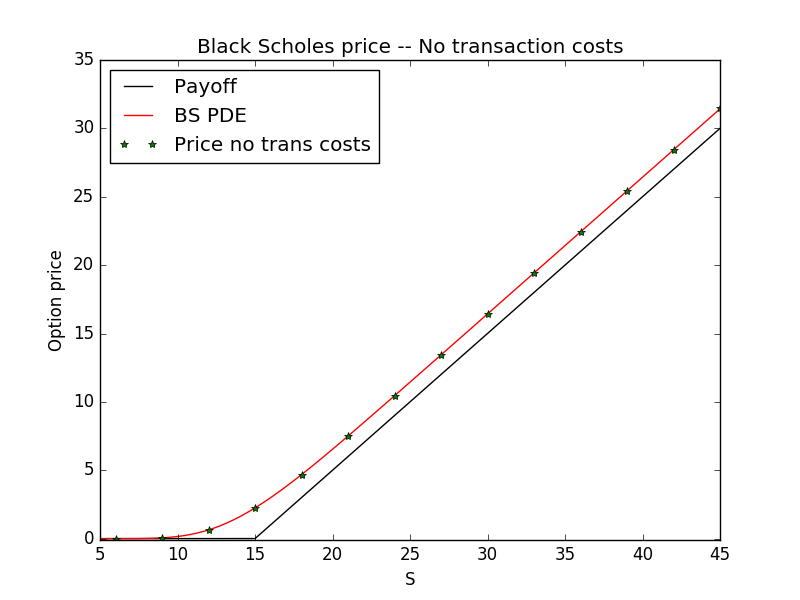
\includegraphics[width=\linewidth]{BS_No_costs.png}
   %\caption{Writer prices with zero transaction costs for diffusion process. Parameters are in the table \ref{tab:BS}.}
   %\label{Fig1} 
 \end{minipage}
 \ \hspace{2mm} \hspace{3mm} \
 \begin{minipage}[b]{0.5\linewidth}
  \centering
   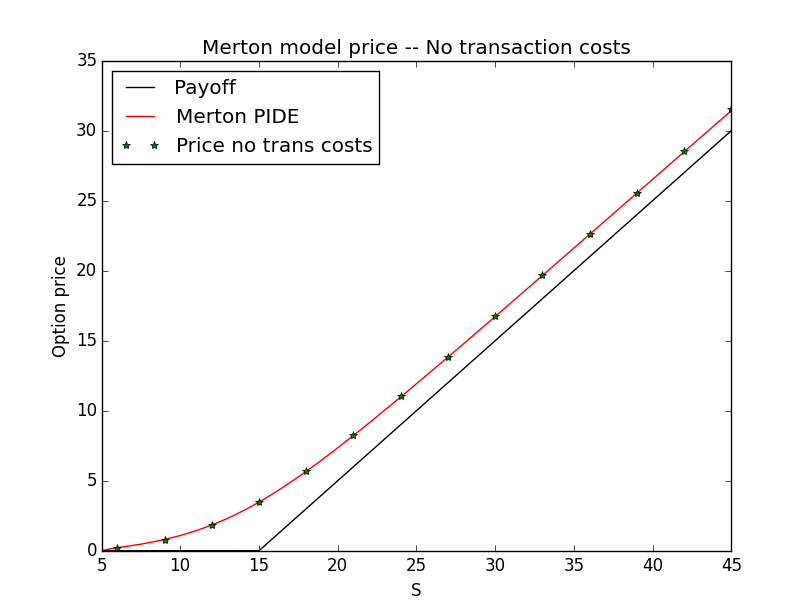
\includegraphics[width=\linewidth]{no_costs.png}
   %\caption{Writer prices with zero transaction costs for Merton process. Parameters are in the table \ref{tab:Mert}.}
   %\label{Fig2}
 \end{minipage}
  \ \hspace{2mm} \hspace{3mm} \
  \begin{minipage}[b]{\linewidth}
  \centering
   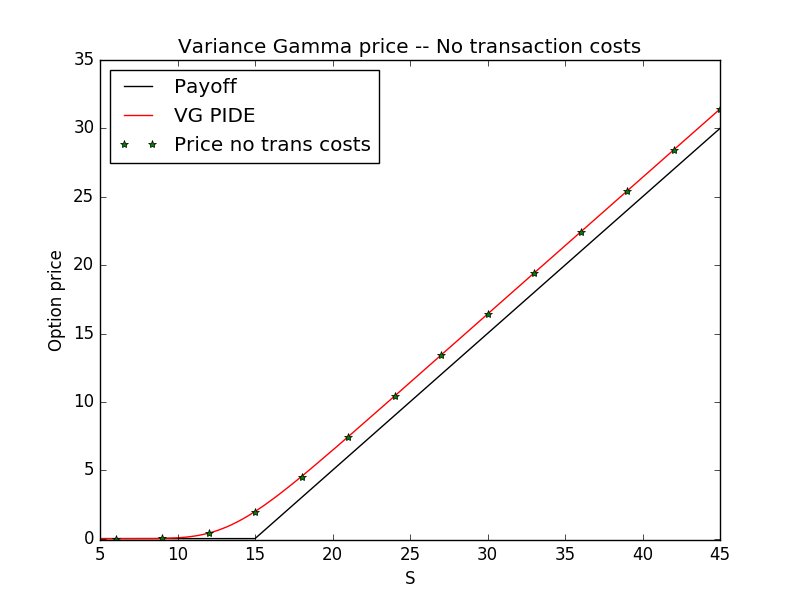
\includegraphics[width=0.51\linewidth]{No_costs_VG.png}
   \caption{Writer prices with zero transaction costs for diffusion (top-left), Merton (top-right) and VG (bottom) process. Parameters are in the table \ref{tab:parameters}.}
   \label{Fig1}
 \end{minipage}
\end{figure}
We compute the option prices using the standard 
\emph{martingale pricing theory} (see Chapter \ref{Chapter2}). In the table \ref{tab:ATM_price} we show the \emph{at the money} values obtained with the closed formula 
and by solving the respective PIDE. 
The closed formula for the diffusion process is the well known \cite{BS73} formula. To compute the Merton price we use the series approximation formula derived in \cite{Me76},
and for the VG price we used the semi-closed formula derived in \cite{MCC98}. The PIDE prices are obtained by solving the equations (\ref{BS_PDE}), (\ref{Merton_PIDE}) and (\ref{VG_PIDE}).
Of course, the parameter $\mu$ has not been used to compute the prices in Tab. \ref{tab:ATM_price}. In Section (\ref{properties_model}), we prove with a numerical experiment that
even though the portfolio process (\ref{portfolio_dynamics2}) has a drift parameter $\mu$, it does not play an important role for the option price.
In the following analysis, we consider the PIDE prices as our benchmarks for comparisons.   
In all the computations we use equal transaction costs for buying and selling, $\theta_b = \theta_s$.

%%%%%%%%%%%%%%%%%%%%%%%%%%%%%%%%%%%%%%%%%%%%%%%%%%%%%%%%%%%%%%%%%%%%%%%%


In Fig. \ref{Fig1} we show that model prices replicate the PIDE prices for zero transaction costs and small values of $\gamma$. 
The values of $\gamma$ in the table \ref{tab:parameters},
are chosen very small\footnote{ In chapter 5 of \cite{GK99} are presented some common values for the risk aversion coefficient: $\gamma=0.3$, $\gamma=0.2$ and $\gamma=0.1$ 
for high, medium and low level of risk aversion respectively.} on purpose. 
An intuitive argument to justify this choice is that for $\gamma \to 0$, the utility function 
can be approximated by a linear utility $\mathcal{U}(w) = 1 - e^{-\gamma w} \approx \gamma w$ and the investor can be considered risk neutral. 
For more details we refer to \cite{Carmona} and references therein. 
\begin{figure}[t!]
 \begin{minipage}[b]{0.5\linewidth}
   \centering
   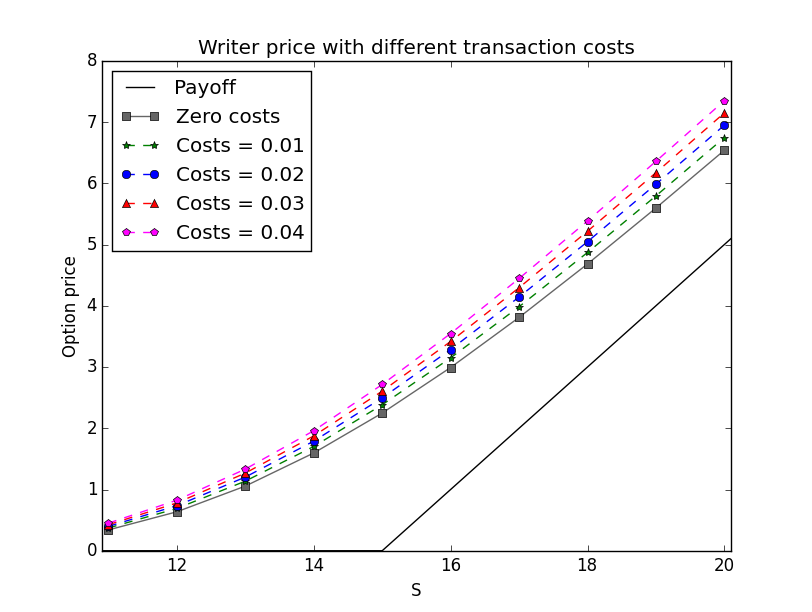
\includegraphics[width=\linewidth]{Trinomial_writer.png}
%   \caption{Writer prices for different transaction costs. The continuous line is the solution of the Black-Scholes PDE.}
%   \label{Fig4} 
 \end{minipage}
 \ \hspace{2mm} \hspace{3mm} \
 \begin{minipage}[b]{0.5\linewidth}
  \centering
   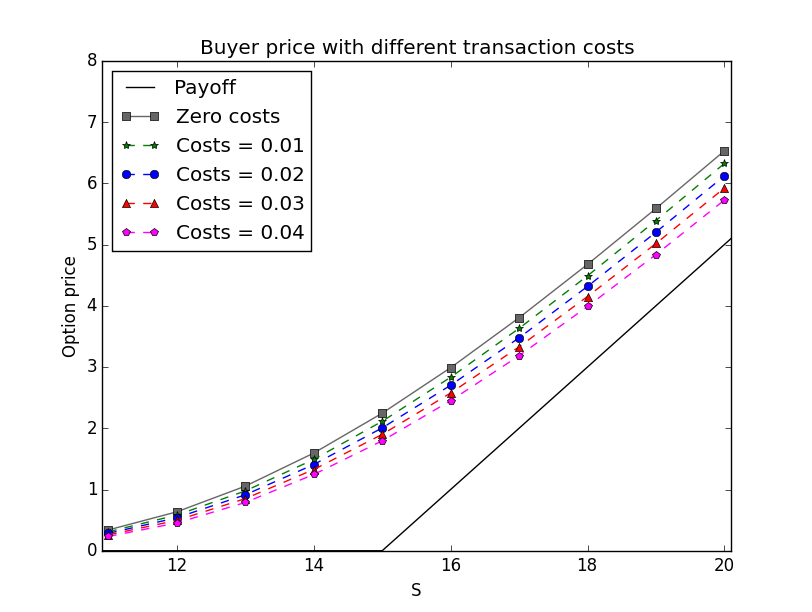
\includegraphics[width=\linewidth]{Trinomial_buyer.png}
 \end{minipage}
    \caption{Writer and buyer prices for different levels of transaction costs. The continuous line is the solution of the Black-Scholes PDE.}
   \label{Fig2}
\end{figure}

\begin{table}[ht]
\centering
 \begin{tabular}{*{11}l}
 \toprule
  \multicolumn{5}{c}{\textbf{Convergence table}} \\
  \midrule
  $N = \bar M$ & $\gamma = 0.0001$ & $\gamma = 0.001$ & $\gamma = 0.01$ & Execution time \\
  \midrule
    50   & 2.241214 & 2.241764 & 2.247311 & 0.01 $\pm$ 0.004\\
    100  & 2.249142 & 2.249506 & 2.253159 & 0.02 $\pm$ 0.005\\
    200  & 2.245422 & 2.245676 & 2.248216 & 0.11 $\pm$ 0.02\\
    400  & 2.246784 & 2.246959 & 2.248717 & 0.85 $\pm$ 0.04 \\
    800  & 2.246288 & 2.246271 & 2.247635 & 8.63 $\pm$ 0.1 \\
    1600 & 2.246576 & 2.246662 & 2.247515 & 82.44 $\pm$ 2.71\\
    3200 & 2.246412 & 2.246471 & 2.247068 & 910.8 $\pm$ 10.5\\
    3500 & 2.246366 & 2.246423 & 2.246993 & 1291.3 $\pm$ 13\\
  \bottomrule
  \end{tabular}
  \caption{Convergence table for ATM diffusion prices with zero transaction costs.}
  \label{tab:convergence}
\end{table}

\subsection{Diffusion results}

In the figure \ref{Fig2} we show the diffusion writer and buyer prices with different
transaction costs.  
We can see that a higher transaction cost corresponds to a higher writer price, while a lower transaction cost corresponds to a lower buyer price.
In fact, the writer and buyer prices are respectively increasing and decreasing functions of the transaction cost, as already verified in \cite{ClHo97}.
The prices figures \ref{Fig2}, are calculated with $N=1500$ time steps and $\bar M = N$. 
In the Table \ref{tab:convergence} we show ATM option prices for different values of $N$, with $\theta_s = \theta_b = 0$ and different risk aversion coefficients.
For $\gamma=0.0001$ and $N=3500$ the price is identical, up to the fourth decimal digit, to the original Black-Scholes price in table \ref{tab:ATM_price}. 
Using the values in the table \ref{tab:convergence} it is possible to estimate the \emph{rate of convergence}.
We also present the execution times, from which we can estimate the asymptotic \emph{time complexity} of the algorithm. 
In Section (\ref{algorithm_Sect}) we estimated a complexity of $\mathcal{O}(N^{4})$. From the table \ref{tab:convergence}, 
we obtain the exponent $\frac{\log(1291.3/910.8)}{\log(3500/3200)} = 3.9$, which is very close to the predicted value.  
The algorithm is written in Matlab using vectorized operations, and runs on an Intel i7 (7th Gen) with Linux.

\subsection{Merton results}

\begin{figure}[t!]
 \begin{minipage}[b]{0.5\linewidth}
   \centering
   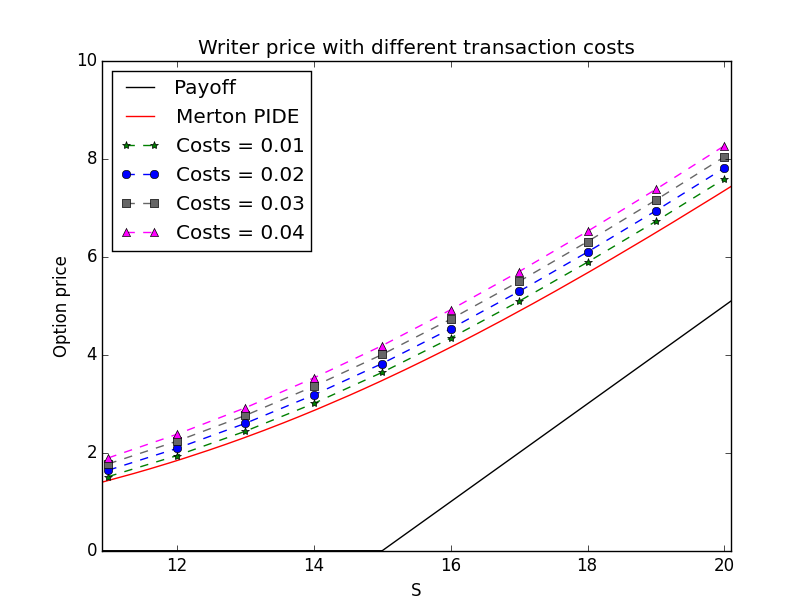
\includegraphics[width=\linewidth]{writer_cost.png}
 %  \caption{Writer prices for different transaction costs. The continuous line is the solution of the Merton PIDE.}
 %  \label{Fig6} 
 \end{minipage}
 \ \hspace{2mm} \hspace{3mm} \
 \begin{minipage}[b]{0.5\linewidth}
  \centering
   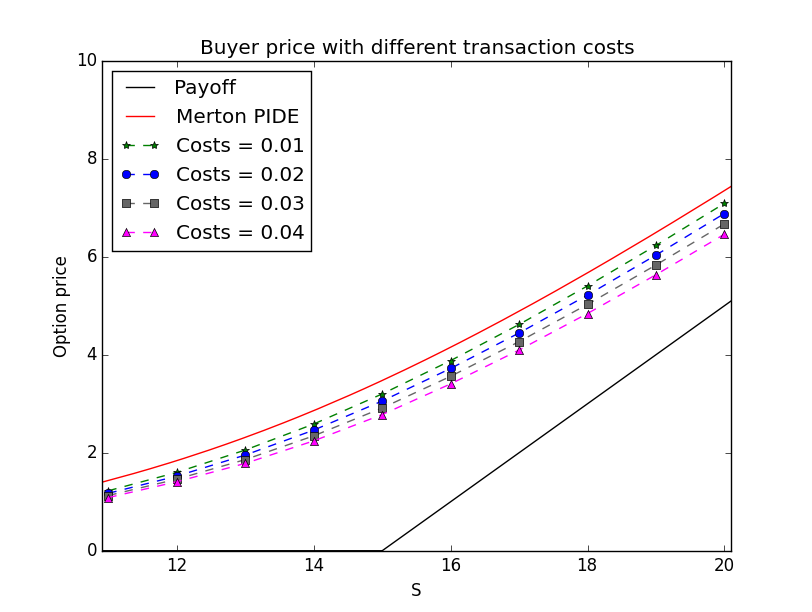
\includegraphics[width=\linewidth]{Price_buyer.png}
 \end{minipage}
 \caption{Writer and buyer prices for different transaction costs. The continuous line is the solution of the Merton PIDE.}
   \label{Fig3}
\end{figure}
In the Figure \ref{Fig3} we show the writer and buyer prices for the Merton process, with parameters in Tab. \ref{tab:parameters}.
An interesting feature of the multinomial tree construction for jump-diffusion processes is that $\bar L \propto \sqrt{N}$.
The integral domain is restricted to the bounded domain $[-B_1,B_2]$ with length $B_1+B_2 = \bar L \, h_x$. 
We choose the size of a space step as $h_x = \sqrt{\E[\Delta X^2]} = \sigma_X \sqrt{\Delta t}$ and $\sigma_X^2 = \sigma^2 + \int_{-B_1}^{B_2} z^2 \nu(dz)$.
However, the size of the Poisson jumps does not scale with $\Delta t$. So the number $\bar L$ has to be chosen big enough in order 
to have $L\, h_x \geq B_1+B_2$. 

In general, for a fixed $h_x$, the interval $[-B_1,B_2]$ should be chosen as big as possible. In practice, the choice of the truncation depends on the shape of the L\'evy measure.  
The figures \ref{Fig13}, \ref{Fig14} show two examples where we choose $[-B_1,B_2] = [\xi,\xi]$ and $[-B_1,B_2] = [-3\xi,3\xi]$ respectively. These choices correspond to 
$\bar L = 19$ and $\bar L = 59$.
For the Merton L\'evy measure (a scaled Normal distribution), a good choice is $[-B_1,B_2] = [-3\xi,3\xi]$, with length $\bar L \, h_x = 6\xi$. 
It is well known that the integral over this region is about the $99.74\%$ of the total area.      
Using this interval and the parameters in Tab. \ref{tab:parameters} we obtain the relation $\bar L \geq 5.86 \sqrt{N}$.
In the calculation of the Merton prices in Fig. \ref{Fig3}, we used a discretization with $N=\bar M =100$, and $\bar L = 81$, 
with a good balance between small computational time and small price error. 
\begin{table}[ht]
\centering
 \begin{tabular}{*{6}l}
 \toprule
  \multicolumn{6}{c}{\textbf{Truncation error table}} \\
  \midrule
  $N$ & $\bar L=51$ &   $\bar L=71$   & $\bar L=91$ & $\bar L=101$ & $\bar L=111$ \\
  \midrule
    50   & 3.481318 & 3.481616 & 3.481617 & 3.481617 & 3.481617  \\
    100  & 3.468774 & 3.478806 & 3.479141 & 3.479146 & 3.479146  \\
    150  & 3.439090 & 3.474403 & 3.477574 & 3.477714 & 3.477742  \\
    200  & 3.399442 & 3.466338 & 3.476439 & 3.477234 & 3.477457 \\
  \bottomrule
  \end{tabular}
  \caption{Truncation error for ATM Merton prices with zero transaction costs.}
  \label{tab:convergence2}
\end{table}

The convergence Tab. \ref{tab:convergence2} shows different Merton prices for different values of $N$ and $\bar L$.
Looking at the table from left to right, for each fixed $N$ it is possible to note how the truncation error decreases when $\bar L$ increases.
\begin{figure}[t!]
 \begin{minipage}[b]{0.5\linewidth}
   \centering
   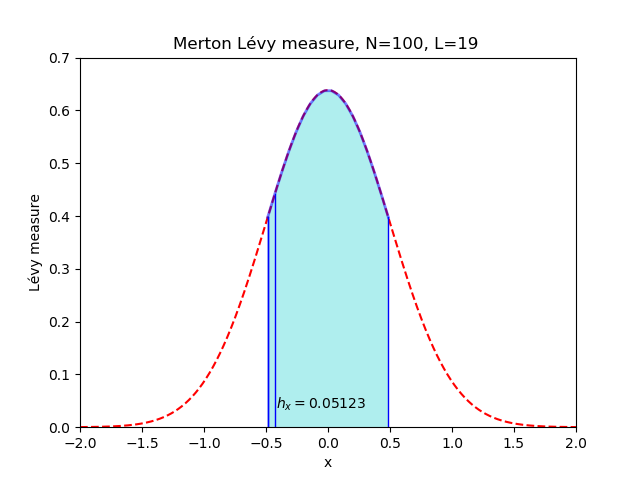
\includegraphics[width=\linewidth]{Mert61_3.png}
   \caption{Merton L\'evy measure computed using parameters in Tab. \ref{tab:parameters}, $N=100$ and $\bar L=19$. 
   The domain $[-B_1,B_2] = [-\xi,\xi]$ has length $\bar L h_x \approx 2 \xi$.}
   \label{Fig13} 
 \end{minipage}
 \ \hspace{2mm} \hspace{3mm} \
 \begin{minipage}[b]{0.5\linewidth}
  \centering
   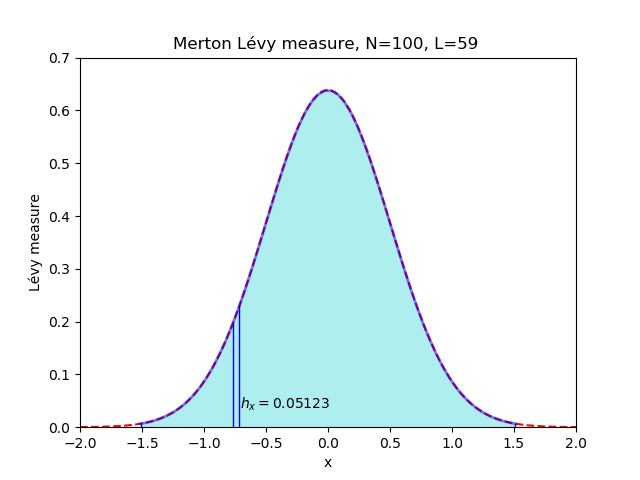
\includegraphics[width=\linewidth]{Mert101_3.png}
   \caption{Merton L\'evy measure computed using parameters in Tab. \ref{tab:parameters}, $N=100$ and $\bar L=59$. 
   The domain $[-B_1,B_2] = [-3\xi,3\xi]$ has length $\bar L h_x \approx 6 \xi$.}
   \label{Fig14}
 \end{minipage}
\end{figure}
\begin{table}[ht]
\centering
 \begin{tabular}{llll}
 \toprule
  \multicolumn{4}{c}{\textbf{Convergence table}} \\
  \midrule
  $N = \bar M$ & $\bar L$ & Price & Execution time \\
  \midrule
    50  & 61  & 3.481600 & 2.20 $\pm$ 0.08 \\
    75  & 75  & 3.479980 & 15.15 $\pm$ 0.07 \\
    100 & 91  & 3.479141 & 63.04 $\pm$ 0.49 \\
    125 & 97  & 3.478254 & 148.4 $\pm$ 1.16 \\
    150 & 105 & 3.477731 & 315.3 $\pm$ 5.58 \\
    175 & 113 & 3.477610 & 585.7 $\pm$ 10.57 \\ 
    200 & 121 & 3.477513 & 1106.0 $\pm$ 12.2 \\
  \bottomrule
  \end{tabular}
  \caption{Convergence table for ATM Merton prices with zero transaction costs.}
  \label{tab:convergence3}
\end{table}


In Table \ref{tab:convergence3} we show several prices with increasing values of $N$ and $\bar L$. We choose $\bar L$ big enough, such that the truncation error can be ignored.
Given the high computational complexity of the algorithm, 
it is difficult to present prices with bigger values of $N$,$\bar L$. For larger values of $N$ and smaller $\gamma$, we expect a convergence to the Merton price in Tab. 
\ref{tab:ATM_price}. 
The computational complexity in this case is expected to be $\mathcal{O}(N^{4.5})$. From the table \ref{tab:convergence3} we get 
the exponent equal to $\frac{\log(1106.0/585.7)}{\log(200/175)} = 4.76$. Considering the errors, the results is not so different from the predicted value.

\subsection{VG results}\label{num_sec_VG}

\begin{figure}[t!]
 \begin{minipage}[b]{0.5\linewidth}
   \centering
   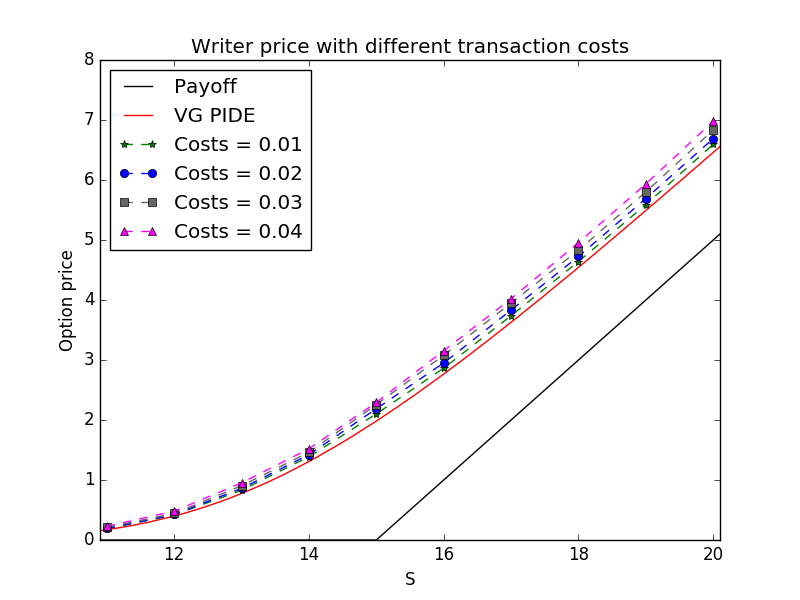
\includegraphics[width=\linewidth]{VG_Writer.png}
   %\caption{Writer prices for different transaction costs. The continuous line is the solution of the VG PIDE.}
   %\label{Fig8} 
 \end{minipage}
 \ \hspace{2mm} \hspace{3mm} \
 \begin{minipage}[b]{0.5\linewidth}
  %\centering
   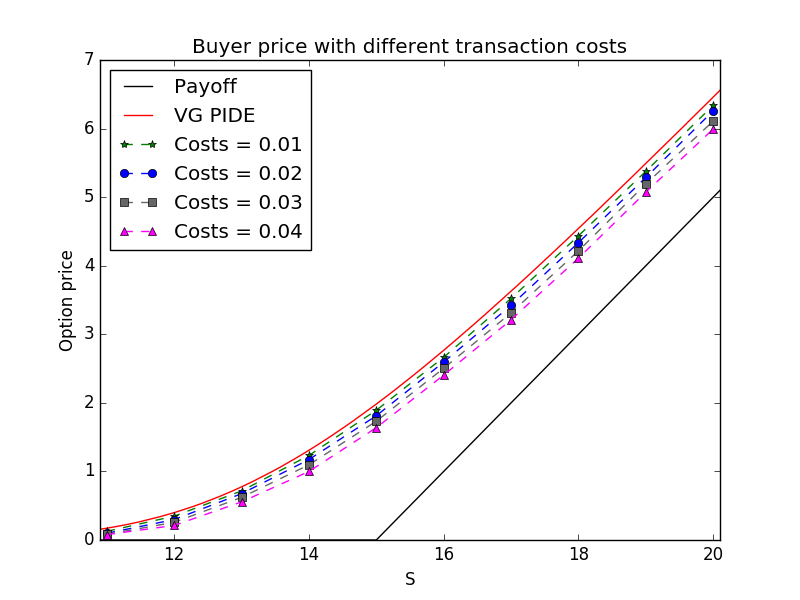
\includegraphics[width=\linewidth]{VG_Buyer.png}
 \end{minipage}
 \caption{Writer and buyer prices for different transaction costs. The continuous line is the solution of the VG PIDE.}
 \label{Fig8}
\end{figure}  

In the Figure \ref{Fig8} we show how the writer and buyer prices for the VG process change for several level of transaction costs (parameters in Tab. \ref{tab:parameters}). 
In these computations we used $N=\bar M = 150$ and $\bar L = 43$, such that the program can run in a reasonable computational time. 
The integration region in \ref{VG_inf_gen} is restricted to $[-B_1,-\epsilon]\bigcup [\epsilon,B_2]$ with $\epsilon=1.5h_x$. The choice of $B_1$ and $B_2$ depends on the shape of the 
L\'evy measure. 
In Fig. \ref{Fig15} and \ref{Fig16} we show two examples for the VG L\'evy measure (using parameters in table \ref{tab:parameters}) with $N=150$, $h_x=0.0165$ and $N=1000$, $h_x=0.0064$. 
The two L\'evy measures are normalized, such that the integral on the region $[-\infty,-\epsilon]\bigcup [\epsilon,+\infty]$ is equal to one. The 
area underlying the functions on $[-B_1,-\epsilon]\bigcup [\epsilon,B_2]$ is highlighted for clarity.
For $\bar L = 43$, we can see that in both cases it is possible to cover a very high percentage of the initial unrestricted region. We can conclude that, unlike the Merton
measure, we do not need a big truncation interval.
Given the space step $h_X = \sigma_X\sqrt{\Delta t}$, with  
$ \sigma_X^2 = \hat \sigma_{J}^2 + \sigma_{\epsilon}^2 $ and $\hat \sigma_J^2 = \int_{[-B_1,-\epsilon]\bigcup [\epsilon,B_2]} z^2 \nu(dz)$, 
it is enough to consider a region at least as big as the standard deviation of the jump process: 
$h_X \bar L \geq \hat \sigma_J$.
Putting all together, the relation becomes $\bar L\geq \frac{\hat \sigma_J}{\sigma_X} \sqrt{N}$, and replacing the values $\sigma_X = 0.2024$ and $\hat \sigma_J=0.1916$ 
we get $\bar L \geq 0.94 \sqrt{N}$.
\begin{table}[ht]
\centering
 \begin{tabular}{llll}
 \toprule
  \multicolumn{4}{c}{\textbf{Convergence table}} \\
  \midrule
  $N = \bar M$ & $\lambda_{\epsilon}$ & Price & Execution time \\
  \midrule
    50  & 4.73  & 1.910934 & 3.63 $\pm$ 0.16 \\
    100 & 7.82  & 1.957806 & 26.54 $\pm$ 0.26 \\
    150 & 10.01 & 1.982078 & 82.51 $\pm$ 0.20 \\
    200 & 11.73 & 1.996180 & 185.2 $\pm$ 0.81 \\
    250 & 13.14 & 2.004719 & 350.3 $\pm$ 4.5 \\
    300 & 14.35 & 2.008536 & 654.2 $\pm$ 7.3\\ 
    350 & 15.40 & 2.009436 & 1236 $\pm$ 12 \\
  \bottomrule
  \end{tabular}
  \caption{Convergence of ATM VG prices with $\bar L =43$, zero transaction costs.}
  \label{tab:convergence4}
\end{table}

In the Table \ref{tab:convergence4} we present several option prices computed with different values of $N$, but with fixed $\bar L$.
In the case of the VG process it is more difficult to analyze the convergence results.
This is due to the approximation (\ref{log_sde_inf_act2}) introduced to replace the infinite activity jump component with a Brownian motion. All the parameters
in (\ref{sig_eps}) depend on $\epsilon$, and consequently on $N$.
Within our discretization ($N=150$), we have $\sigma_{\epsilon} = 0.0654$, $\lambda_{\epsilon} = 10.01$. 
With those parameters we obtain an ATM price for zero transaction costs of 1.9821, which is very close the the PIDE price in Tab. \ref{tab:ATM_price}. 
We expect to have convergence to the PIDE price for $N\to \infty$ and $\gamma\to0$.
When $N \to \infty$ and $\epsilon \to 0$, the parameters $\sigma_{\epsilon} \to 0$ and $\lambda_{\epsilon}\to \infty$.
The main problems are the high dependence of the price on the parameter $\epsilon$ and therefore on the discretization step $h_x$, together with the high complexity of the algorithm.
For instance, with $N=\bar M=1000$ and $\bar L = 43$ the program takes more than two hours to run. 
The convergence of the approximated process (\ref{log_sde_inf_act}) to the original VG process is very slow, and this is reflected in the convergence 
of the VG PIDE (\ref{VG_PIDE}).
In order to solve it (using the IMEX scheme proposed by \cite{CoVo05b}) we constructed
a grid with 13000 space steps of size $\delta x = 0.0004$ and 7000 time steps, and obtained the price in Tab \ref{tab:ATM_price}, 
with the approximated activity $\lambda_{\epsilon} = 75$.
Consequently, we expect to have good convergence results in our algorithm when $N\sim 10^4$.
All the presented prices (Figures \ref{Fig8}) have thus a truncation error, which is adjusted by an accurate choice of the value of $\gamma$. 
We refer to \cite{CoVo05b} for a detailed error analysis.
\begin{figure}[t!]
 \begin{minipage}[b]{0.5\linewidth}
   \centering
   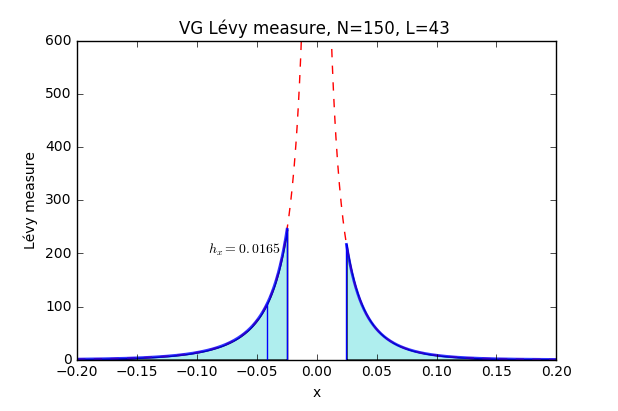
\includegraphics[width=\linewidth]{VG43.png}
   \caption{VG L\'evy measure computed using parameters in Tab. \ref{tab:parameters}, $N=150$ and $\bar L=43$. 
   The domain $[-B_1,-\epsilon]\bigcup [\epsilon,B_2]$ has length $(\bar L-3) h_x$. The highlighted area is $99.9\%$ of the total area.}
   \label{Fig15} 
 \end{minipage}
 \ \hspace{2mm} \hspace{3mm} \
 \begin{minipage}[b]{0.5\linewidth}
  \centering
   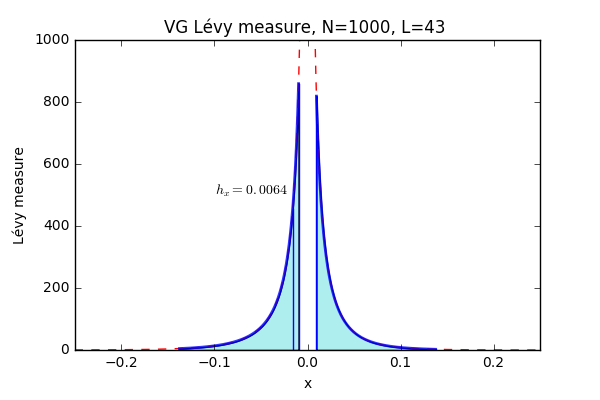
\includegraphics[width=\linewidth]{VG1000.png}
   \caption{VG L\'evy measure computed using parameters in Tab. \ref{tab:parameters}, $N=1000$ and $\bar L=43$. 
   The domain $[-B_1,-\epsilon]\bigcup [\epsilon,B_2]$ has length $(\bar L-3) h_x$. The highlighted area is $98.9\%$ of the total area.}
   \label{Fig16}
 \end{minipage}
\end{figure}

From Tab. \ref{tab:convergence4} we can estimate the time complexity of this algorithm. The exponent is $\frac{\log(1236.0/654.2)}{\log(350/300)} = 4.12$, 
indeed very close to the theoretical $\mathcal{O}(N^4)$. 



\subsection{Properties of the model}\label{properties_model}

\begin{table}[ht]
  \centering
 \begin{tabular}{llllll}
\toprule
 & cost = 0 & cost = 0.01 & cost = 0.02 & cost = 0.03 & cost = 0.04  \\
\midrule
\textbf{Merton} & 3.4771 & 3.6400 & 3.8212 & 4.0054 & 4.1864 \\
\textbf{VG} & 1.9821 & 2.0921 & 2.1870 & 2.2568 & 2.3131 \\
\bottomrule
\end{tabular}
  \caption{Merton and VG writer prices for different transaction costs, with parameters as in Tab. (\ref{tab:parameters}). }
  \label{tab:costs}
\end{table}

In this section we want to analyze the properties of the model and how the option price depends on the level of transaction costs $\theta_b$, $\theta_s$, 
the risk aversion parameter $\gamma$ and the drift $\mu$. 
In this numerical experiment, we use the Merton model with parameters of Tab. \ref{tab:parameters}.
In Tab. \ref{tab:costs} we show the writer ATM option values for different transaction costs.  
\begin{figure}[t!]
 \begin{minipage}[b]{0.5\linewidth}
   \centering
   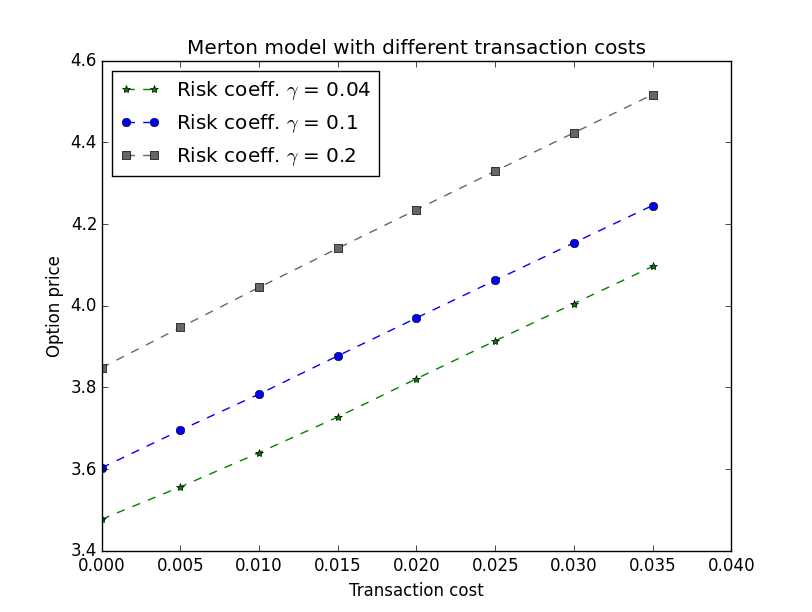
\includegraphics[width=\linewidth]{P_vs_cost.png}
   \caption{Merton option prices for the writer as function of the transaction cost, with different values of $\gamma$.}
   \label{Fig10} 
 \end{minipage}
 \ \hspace{2mm} \hspace{3mm} \
 \begin{minipage}[b]{0.5\linewidth}
  \centering
   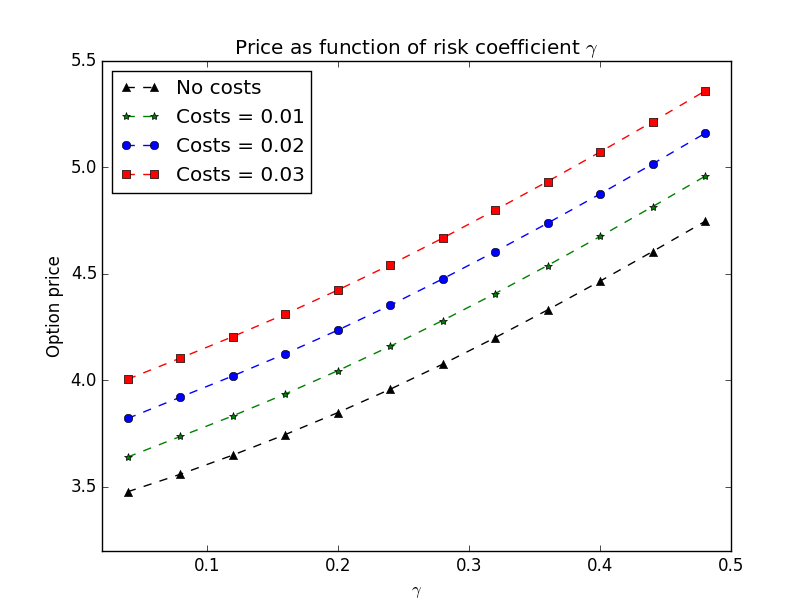
\includegraphics[width=\linewidth]{price_gamma.png}
   \caption{Merton option prices for the writer as function of $\gamma$, with different values of transaction costs.}
   \label{Fig11}
 \end{minipage}
  \ \hspace{2mm} \hspace{3mm} \
  \begin{minipage}[b]{\linewidth}
  \centering
   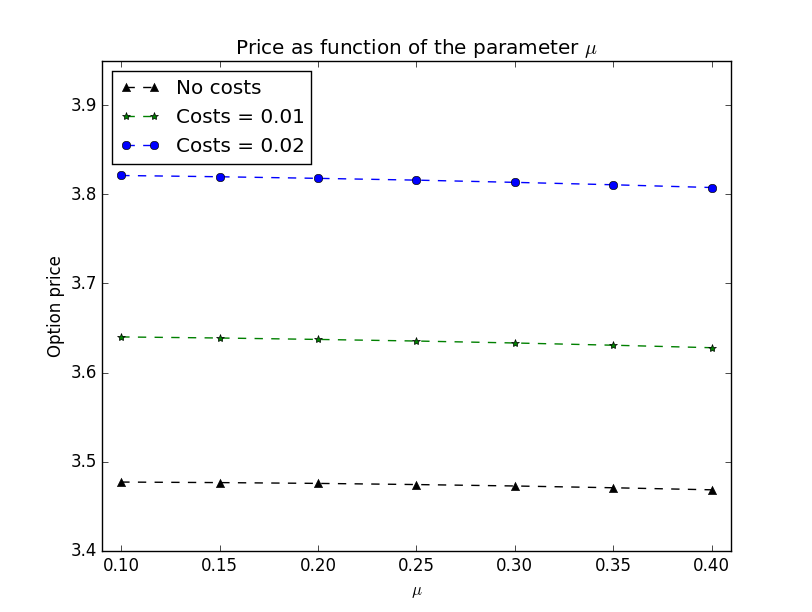
\includegraphics[width=0.55\linewidth]{price_mu2.png}
   \caption{Merton option prices for the writer as function of $\mu$, with different values of transaction costs.}
   \label{Fig12}
 \end{minipage}
\end{figure}


In Fig. \ref{Fig10} we can see better how the price for the writer is affected by the change of the transaction costs. 
The picture shows prices for different values of risk coefficient.
The risk profile of the investor also plays an important role. As already shown in \cite{HoNe89}, the writer price is an
increasing function of the risk aversion coefficient. Figure \ref{Fig11} confirms their results.

In all the previous computations we always used the drift term $\mu$ equal to the risk free interest rate $r$. This is the choice   
made in \cite{HoNe89}, following the common rule of the standard no-arbitrage
theory.
The option price has to be independent of the expected return of the underlying asset.
As we can see in Fig. \ref{Fig12}, the numerical experiment shows that also in this model, the option prices 
do not depend on the drift $\mu$.



\section{Solution of the 4-dimensional problem}

This section focuses on the original HJB equation \ref{HJB1}, were no variables reduction is considered. 
A few authors have already presented some results for the diffusion case, using different approaches.
In \cite{Pal15} the authors propose a method to improve the performances of the Markov chain approximation method for the diffusion case. In \cite{Song14} the author propose
a penalty method for the diffusion case of the 4 dimensional HJB equation, but the numerical results they present are not very clear.

If we want to solve the problem (\ref{max_probl1}), we have to deal with a three dimensional state. In the variable reduction section \ref{variable_reduction}
we assumed a high value of credit availability $C$, such that the default probability can be ignored. 
Here we do not ignore the default case, and compute option prices for investor with low credit availability.
We work with the original problem (\ref{max_probl1}) and derive a discrete time dynamic programming equation as done for (\ref{HJB3}).

Let us indicate with $B_n := B(t^-_n)$ the value of cash immediately before the possible transaction.
Let us define $\Sigma_b := \{-K_5 h_b , ... , -h_b,0,h_b, ... , +K_6 h_b \}$,  
where $h_b>0$ is the discrete cash step and  $K_5,K_6 \in \N$. Its dimension is $\bar B = \#(\Sigma_b) = K_5+K_6+1$.
The discretized SDE for the cash account process $\{B_t\}_{t \in [t_0,T]}$ in (\ref{porfolio_dynamics}), with solution (\ref{BT}), is:
\begin{equation}\label{Bn}
 B_{n+1} =  e^{r \Delta t} \biggl( B_n - (1+\theta_b) e^{X_n} \Delta L_n + (1-\theta_s) e^{X_n} \Delta M_n \biggr)
\end{equation}
Let us derive the backward algorithm for computing the value function using the DPP, as we did for (\ref{HJB3}). %The integral representation of \ref{HJB1} is:
We obtain the discrete DPE: 
\begin{align}\label{HJB5}
 & V(t_n,B_n,Y_n,X_n) = \max \; \biggl\{ \E_n 
 \biggl[ V \bigl( t_{n+1}, e^{r \Delta t} B_n, Y_n, X_n + \Delta X_n \bigr) \biggr], \\ \nonumber
 & \max_{\Delta L_n} 
 \E_n \biggl[ V \bigl( t_{n+1}, e^{r\Delta t}(B_n - e^{X_n}(1+\sigma_b)\Delta L_n) , Y_n + \Delta L_n, X_n + \Delta X_n \bigr) \biggr] , \\ \nonumber
 & \max_{\Delta M_n}
 \E_n \biggl[ V \bigl( t_{n+1}, e^{r\Delta t}(B_n + e^{X_n}(1-\sigma_s)\Delta M_n) , Y_n - \Delta M_n, X_n + \Delta X_n \bigr) \biggr]
 \biggr\},
\end{align}
where all the expectations are conditioned on the current state $(B_n,Y_n,X_n)$.  We use the notation $V(t_n, b_h, y_j, x_i) = V^n_{h,j,i}$

The algorithm \ref{algo2} is very computationally expensive. Since it has one degree of freedom more than the algorithm in Section \ref{algorithm_Sect}, the computational complexity is 
$$\mathcal{O}\biggl( (N+1)\bigl[\frac{N(\bar L-1)}{2}+1 \bigr] \times \bar M \times \bar B \times \sum_{n,h,j,i} \bigl( \# \varPi(t_n,b_h,y_j,x_i) \bigr)  \biggr).$$
The term $\sum_{n,h,j,i} \bigl( \# \varPi(t_n,b_h,y_j,x_i) \bigr)$ is the computational complexity of the minimum search in the entire algorithm. 
The minimum search algorithm is performed for each $(t_n, b_h,y_j,x_i)$ on the set $\varPi(t_n,b_h,y_j,x_i)$ of all $l,m \in \N$ such that:
$$ y_j+l h_y \in \Sigma_y \bigcap (b_h - e^{x_i}(1+\sigma_b)l h_y) \geq -K_5 h_b $$ 
and 
$$y_j-m h_y \in \Sigma_y \bigcap (b_h + e^{x_i}(1-\sigma_s)m h_y) \leq K_6 h_b .$$ 

In the following analysis of the problem (\ref{max_probl1}), we assume that $\mathcal{U}(w) = -C$ for $w < -C$ and $\beta = r$. 
In figure (\ref{Fig21}) it is possible to see the shape of the value function at terminal time for different values of gamma.
In the points $(b,y,x)$ such that $\mathcal{W}(b,y,x) = -C$ the function is not differentiable, and this may create some instabilities in the numerical computations. However this 
assumption will be useful in order to speed up the algorithm.

\begin{figure}[t!]
   \centering
   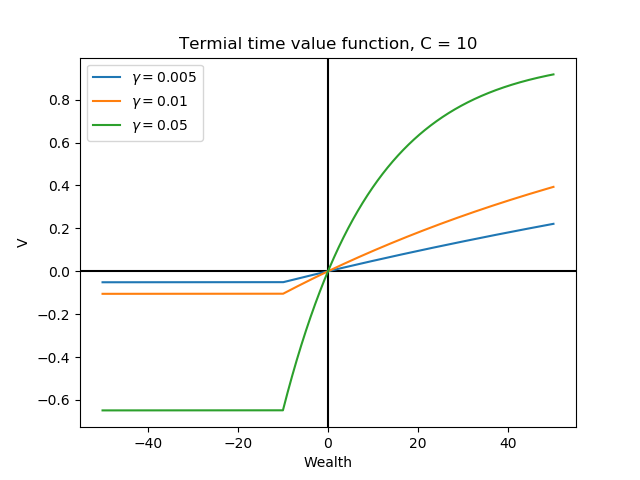
\includegraphics[width=0.7\linewidth]{terminal_utility.png}
   \caption{Terminal time value functions with $\mathcal{U}(w) = -C$ for $w < -C$.}
   \label{Fig21} 
\end{figure}

\begin{algorithm}[H] 
\caption{Backward algorithm}
\label{algo2}
 \algsetup{indent=1.5em}
 \begin{algorithmic}[1]
    \REQUIRE $r, (b,\sigma,\nu), X_0, K, T, \theta_b, \theta_s, \gamma, N, \bar L, \bar M, \bar B. $
    \ENSURE $V^j(t_0,b,y,X_0)$ for $j=0,w,b$
      \STATE Create the lattice for (\ref{log_sde_discr}) and (\ref{Bn}) with appropriate discrete steps $\Delta t, h_y, h_x, h_b$.
      \STATE Create the vector of probabilities $p_k$ as defined in \ref{pK}.  
      \STATE Use (\ref{terminal_conditions}) to initialize a $\bar B \times \bar M \times \bigl( N(\bar L-1)+1 \bigl)$ grid for $V^N_{h,j,i}$.  
      \FOR {n = N-1 to 0}
      \STATE $W_{h,j,i} = \sum_{k = -K_1}^{K_2} p_k \; V^{n+1}_{h,j,i+k}$
      \STATE Interpolate the value of $W$ in the points: \\
             - $W_1(n,h,j,i) \mbox{ at } (t_n, e^{r \Delta t} b_h, y_j, x_i)$.\\
             - $W_2(n,h,j,i,l)$ at $(t_n, e^{r\Delta t}(b_h - e^{x_i}(1+\sigma_b)l h_y), y_j+l h_y, x_i ) $ for each $l$.\\
             - $W_3(n,h,j,i,m)$ at $(t_n, e^{r\Delta t}(b_h + e^{x_i}(1-\sigma_s)m h_y), y_j-m h_y, x_i ) $ for each $m$. 
      \STATE $V^{n}_{h,j,i} = \max \biggl\{ W_1(n,h,j,i), \, \max_l W_2(n,h,j,i,l), \, \max_m W_3(n,h,j,i,m)  \biggr\}$ 
      \ENDFOR
  \end{algorithmic}
\end{algorithm} 

We present numerical solution for a Merton process with values in table \ref{tab:Mert}. 
The cash vector is is chosen such that $-20 \leq B_0 \leq 20$, and consider values of $N = \bar M = \bar B = 25$ and $\bar L = 11$, 
but even with these small values, the algorithm takes about 2 hours to run. 
The algorithm is written in Python and run on a Linux machine with a i7 processor. In order to increase the speed of the program
it is necessary to write the program in a low level language such as C of Fortran.
\begin{figure}[t!]
   \centering
   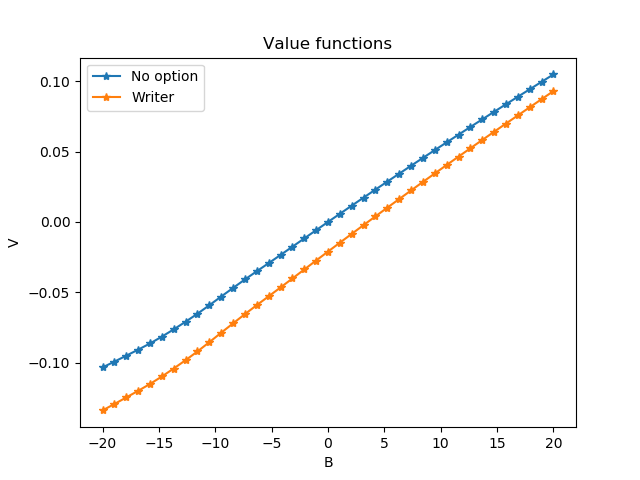
\includegraphics[width=0.6\linewidth]{value_f_C5000.png}
   \caption{Value function for the writer and value function with no option at time $t_0$ with $Y_0=0$ and $S_0=15$. The option price at $B_0=0$ is $p^w=3.48303858$.}
   \label{Fig22} 
\end{figure}

In the figure \ref{Fig22} we computed the value functions and the option prices for $C= 5000$.
The value functions are smooth and, as expected, the option price (defined in (\ref{writer}) ) corresponding to the horizontal distance between the value functions,
is not affected too much by the initial wealth. 
The high value of the credit availability $C$ 
has to be intended as a low default probability. Therefore the problem leads back to the problem with 3 variables. And the numerical results confirm it.

A different story happens when we choose a small credit availability. For example $C = 10$.\\ 
In figure \ref{Fig23} we can see that the two value functions have the same value for $B_0 < -C$, because in this region the value function corresponds to the boundary conditions
(remember that we are considering $Y_0=0$). 
For higher values of $B_0$, the influence of the boundary conditions decreases and the value functions look like those in figure \ref{Fig22}.
\begin{figure}[t!]
 \begin{minipage}[b]{0.5\linewidth}
   \centering
   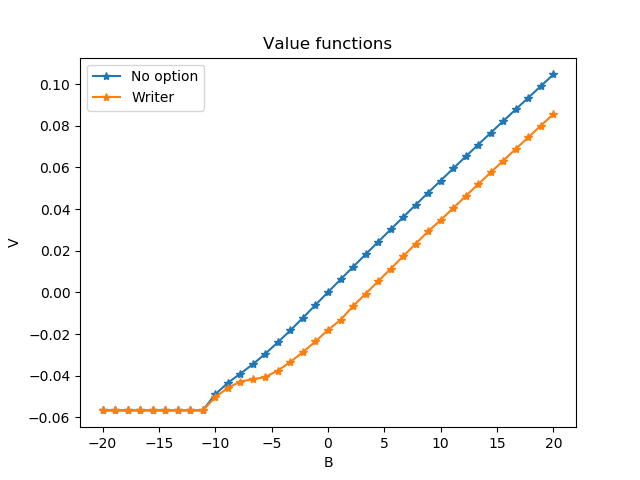
\includegraphics[width=\linewidth]{value_f_C10.png}
   \caption{Writer and no option value functions at $t_0$ with $C=10$, $Y_0=0$ and $S_0=15$.}
   \label{Fig23} 
 \end{minipage}
 \ \hspace{2mm} \hspace{3mm} \
 \begin{minipage}[b]{0.5\linewidth}
  %\centering
   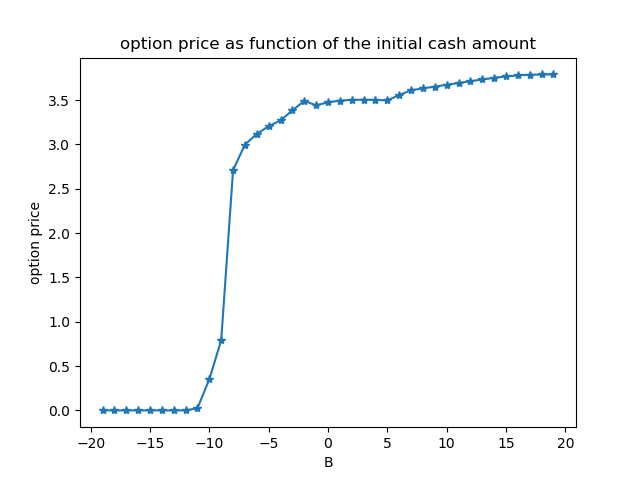
\includegraphics[width=\linewidth]{option_B.png}
   \caption{Option price as function of $B_0$ at $t_0$ with $C=10$, $Y_0=0$ and $S_0=15$.}
   \label{Fig24}
 \end{minipage}
\end{figure}  

It is important to stress that the grid resolution we used in these example is quite rough. The numerical results are still good, but it is not possible at the moment 
to study the convergence properties of the algorithm. 
Furthermore, although the value function is highly non-linear, we used linear interpolation to interpolate the missing points in the grid, and this may create further errors in the shape
of the function and in the final result.

\begin{figure}[t!]
 \begin{minipage}[b]{0.5\linewidth}
   \centering
   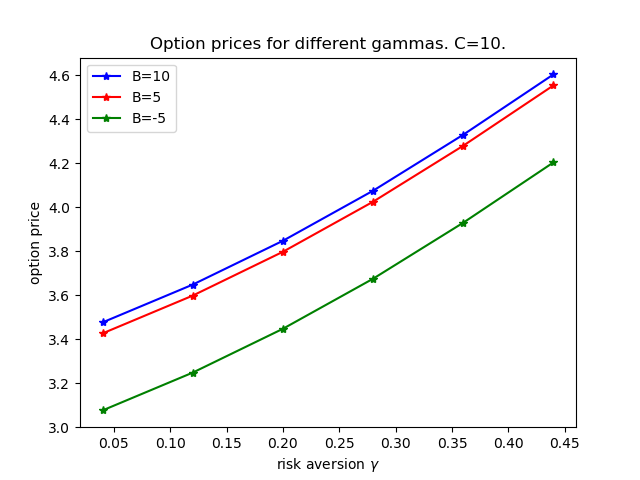
\includegraphics[width=\linewidth]{B_gamma_10.png}
   \caption{Option price as function of risk aversion, for several values of initial $B_0$. We set $C=10$, $Y_0=0$ and $S_0=15$.}
   \label{Fig26} 
 \end{minipage}
 \ \hspace{2mm} \hspace{3mm} \
 \begin{minipage}[b]{0.5\linewidth}
  %\centering
   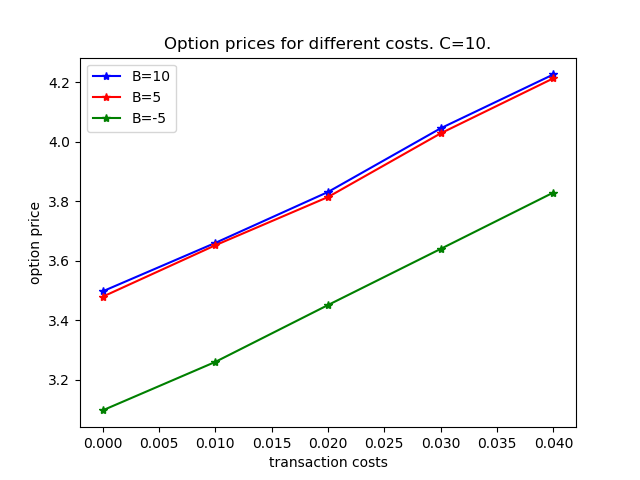
\includegraphics[width=\linewidth]{B_cost_10.png}
   \caption{Option price as function of transaction costs, for several values of initial $B_0$. We set $C=10$, $Y_0=0$ and $S_0=15$.}
   \label{Fig25}
 \end{minipage}
\end{figure}  

We conclude this section by testing the model properties as we did on Section \ref{properties_model}. 
In figures \ref{Fig26} and \ref{Fig25} we present several values of option prices as function of the risk aversion and transaction costs respectively.  
We can see that the value of $B_0$ does not affect the shape of the curve, but only its height. 
As we saw in figures \ref{Fig10} and \ref{Fig11}, the option price is an increasing function of the risk aversion and of the transaction costs.


\section{Multinomial method applied to the reduced problem}

In section \ref{MC_section} we have seen that a possible technique to construct the Markov chain approximation is to discretize the infinitesimal generator of the continuous process
by an explicit finite difference scheme.
For Lévy processes with infinite activity, however, this technique cannot be used directly, and requires to consider the infinitesimal generator of the approximated 
jump-diffusion process.
In the numerical results section \ref{num_sec_VG}, we have seen that the algorithm converges very slowly.

In this section we use the multinomial approximation method presented in chapter \ref{Chapter3}, in place of the discretization obtained by the infinitesimal generator of this chapter.
With this method the total computational complexity is reduced because the number of branches is kept fixed.
Although the method still relies on an approximation (the VG process is approximated by a general jump process with only the first four moments equal),
the number of branches is fixed to $\bar L = 5$, and therefore the computational complexity is reduced by a factor $\sqrt{N}$.
Recall that the complexity for the general reduced variable algorithm is 
$$\mathcal{O}\biggl( (N+1)\bigl[\frac{N(\bar L-1)}{2}+1 \bigr] \times \bar M \times \bar M \biggr).$$
Assuming $\bar M = N$ and $\bar L = 5$, the computation time is reduced to $\mathcal{O}(N^4)$. 
\begin{table}[t!]
\begin{center}
\begin{minipage}{0.8\linewidth}
\centering
 \begin{tabular}{||c|c||}
 \hline
  \multicolumn{2}{|c|}{Convergence table} \\
  \hline
  $N = \bar M$ & Price \\
  \hline
    50 & 1.96121076540 \\
  \hline
    100 & 1.96889900730 \\
  \hline  
    200 &  1.97154200723 \\
  \hline
    400 & 1.97288296067 \\
  \hline   
    800 & 1.97354995910  \\
  \hline
    1000 & 1.97368292970 \\ 
  \hline
    1600 & 1.97388226442  \\
  \hline
    2000 & 1.97394872091  \\  \hline
  \end{tabular}
  \caption{Convergence table for ATM VG prices with parameters in Tab \ref{tab:VG}, calculated with the multinomial method.}
  \label{tab:convergence31}
\end{minipage}
 \end{center}
\end{table}
We use the values in table \ref{tab:VG} and follow the discretization scheme proposed in chapter \ref{Chapter3}. 
In table \ref{tab:convergence31} we reported a convergence analysis.
In the figures \ref{Fig32} and \ref{Fig33} we show how good are the prices computed with the multinomial method. 
\begin{figure}[t!]
 \begin{minipage}[b]{0.5\linewidth}
   \centering
   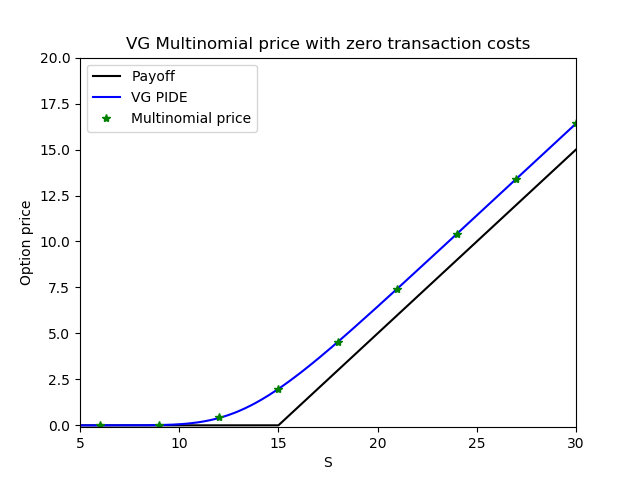
\includegraphics[width=\linewidth]{Multi_VG_zerocosts.png}
   \caption{The multinomial VG prices for zero transaction costs agree with the solution of the VG PIDE (continuous line).}
   \label{Fig32} 
 \end{minipage}
 \ \hspace{2mm} \hspace{3mm} \
 \begin{minipage}[b]{0.5\linewidth}
  %\centering
   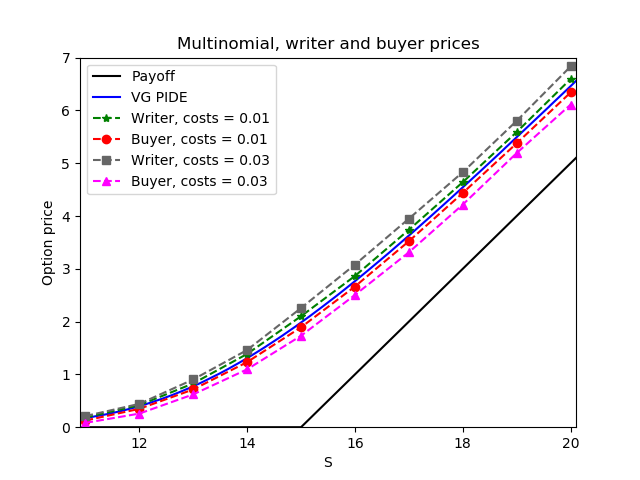
\includegraphics[width=\linewidth]{Multi_VG_costs.png}
   \caption{Multinomial VG writer and buyer prices for different transaction costs.}
   \label{Fig33}
 \end{minipage}
\end{figure}  

	


\chapter{Conclusions}\label{Conclusions}
%\blindtext
%\minitoc% Creating an actual minitoc


\vspace{5em}




The main objective of this thesis is to develop a new model for pricing options in presence of proportional transaction costs.
We propose a model that is a generalization of the model first introduced by \cite{HoNe89} and then formalized by \cite{DaPaZa93}.
The main difference with previous works in the literature is that we are considering a stock dynamics following a generic exponential Lévy process.
Another new feature introduced in our model is the possibility of default for the investor's portfolio. These new features have already been introduced in articles 
concerning portfolio selection problems e.g. \cite{Kab16}, but to our knowledge are completely new in the area of option pricing under transaction costs.
Following the framework of \cite{Kab16}, we present an optimal singular control problem and derive the associated Hamilton-Jacobi-Bellman equation.
In the thesis the option price is defined as the \emph{indifference price}, whose definition is based on the \emph{expected utility maximization} concept.
One of the main theoretical contributions of the thesis is the proof of the existence of a viscosity solution 
for this HJB equation. 

Since the general maximization problem (\ref{max_probl1}) is quite complex and its numerical solution is computationally expensive,
we considered also the special case of an investor with a very large \emph{credit availability} i.e. the possibility of default is ignored.
Under this assumption it is possible to reduce the number of variables of the problem. We then obtained the simplified problem (\ref{minimization}), 
with the associated HJB equation (\ref{HJB2}).
We proposed a numerical scheme and proved that it is a monotone, stable and consistent scheme.  
Moreover, we proved that its solution converges to the viscosity solution of the
HJB equation (\ref{HJB2}). This is another important theoretical contribution of the thesis.

Numerical solutions are provided for both the HJB equations (\ref{HJB2}) and (\ref{HJB1}). 
More emphasis was given to (\ref{HJB2}) where we presented several numerical results for different Lévy processes and we provided convergence and time complexity 
analysis.
Numerical examples are provided for three different Lévy processes: the Brownian motion, the Merton jump-diffusion and the Variance Gamma processes. 
We compared the results of our model with the prices obtained with the martingale pricing theory.
We verified that for small risk aversion and for zero transaction costs, our model is able to replicate those prices with good precision.

The main numerical approach used in the thesis is the \emph{Markov chain approximation} method. We explain how to construct the approximated Markov chain from the 
discretization of the infinitesimal generator of the continuous time process.
We showed that the Brownian motion and the Merton process can be discretized directly, 
while the VG process needs to be approximated to remove the infinite activity jump component.
We also present results obtained with the multinomial method of \cite{YaPr01} for the Variance Gamma process. In this case, there is no need to discretize the infinitesimal
generator in order to construct the Markov chain approximation, and the computational complexity of the method is smaller. 


To conclude, we want to mention some possible future improvements in this area of research. 
An interesting direction can be the development of a more efficient numerical method for the HJB equations (\ref{HJB2}), and in particular for (\ref{HJB1}), 
which has a huge time complexity.
There are several approaches in the literature to solve variational inequalities, such as the policy iteration method of \cite{FoHu12a}, or the penalty method of 
\cite{FoHu12b}, \cite{Song14}.
We argue that an implicit/explicit (IMEX), with the possible help of the Fast-Fourier-Transform for evaluating the integral term (as in \cite{AnAn00} for instance) 
can increase the efficiency of the numerical method.
Also, using a non-uniform grid as in \cite{Haentjens13}, can help to improve the efficiency 
and reduce the computational cost for both the differential and the integral part.






\section*{Acknowledgements}

First of all, I want to thank my PhD supervisors Prof. João Guerra and Prof. Manuel Guerra for the
patience they had with me, for the useful discussions and the many emails we have exchanged in recent years.
I would like to express my thanks to Prof. Maria do Rosário Grossinho, who gave me the opportunity to start
this doctoral program together with the European network STRIKE \url{http://www.itn-strike.eu/} and who has always 
given me positive energy.
Last, but not least, I want to thank my family and my friends Pedro Polvora, Yaser Faghan Kord, Radoslav Vulkov, 
Daniele Polencic and Alessandro Scalia for their never-ending support.

This research was supported by the European Union in the FP7-PEOPLE-2012-ITN project STRIKE - 
Novel Methods in Computational Finance (304617), and by CEMAPRE
MULTI/00491, financed by FCT/MEC through Portuguese national funds.





%\pagenumbering{roman}
%\frontmatter
%\mainmatter


\bibliographystyle{apalike}
\bibliography{/home/nicola/Documenti/ISEG/Bibliografia/trans_cost.bib,/home/nicola/Documenti/ISEG/Bibliografia/book.bib,/home/nicola/Documenti/ISEG/Bibliografia/fin_math.bib,/home/nicola/Documenti/ISEG/Bibliografia/viscosity.bib,/home/nicola/Documenti/ISEG/Bibliografia/num_meth.bib,/home/nicola/Documenti/ISEG/Bibliografia/phd_thesis.bib,/home/nicola/Documenti/ISEG/Bibliografia/Levy.bib,/home/nicola/Documenti/ISEG/Bibliografia/control.bib}

%test git

\end{document}
